\documentclass{amsart}
%\usepackage[backend=bibtex8,style=numeric,giveninits=true]{biblatex}
%\addbibresource{formschub.bib}
\usepackage{algorithm}
\usepackage{algpseudocode}
\usepackage{hyperref}
\usepackage{fancyvrb}
\usepackage{amsmath}
\usepackage{amsfonts}
\usepackage{amsthm}
\usepackage{amssymb}
\usepackage{array}
\usepackage{cases}
\usepackage{caption}
\usepackage{xcolor}
\usepackage{tikz}
\usepackage{tikz-cd}
\usepackage{mathtools}
\usetikzlibrary{calc}
\usepackage{centernot}
\usepackage{mathtools}
\usepackage{graphicx}
\usepackage[margin=1in]{geometry}
\usepackage[makeroom]{cancel}
\usepackage{stmaryrd}
\usepackage{stackengine}
\usepackage{mathrsfs}

% Concatenation product on \dcoma: a square cup with a + inside (visually `\sqcupplus`).
\makeatletter
\newcommand{\sqcupplus@inner}[2]{%
  \vcenter{\hbox{\ooalign{%
    \hfil$\m@th#1\sqcup$\hfil\cr
    \hfil\raisebox{0.15ex}{$\m@th#1\scriptscriptstyle+$}\hfil\cr
  }}}%
}
\newcommand{\sqcupplus}{\mathbin{\mathpalette\sqcupplus@inner\relax}}
\makeatother

%\usepackage{unicode-math}
%\usepackage{nicematrix}

%\usepackage{witharrows}

\newtheorem{lemma}{Lemma}[subsection]
\newtheorem{corollary}[lemma]{Corollary}

\newtheorem{proposition}[lemma]{Proposition} 
\newtheorem{proposition2}{Proposition}[section]
\newtheorem{theorem}{Theorem}[section]
\newtheorem{conjecture}[theorem]{Conjecture} 
\newtheorem{observation}{Observation}[section]
\newtheorem{question}{Question}

%\newtheorem{conj}[thm]{Conjecture} 


%%% 
%%% The following gives definition type environments (which only differ
%%% from theorem type invironmants in the choices of fonts).  The
%%% numbering is still tied to the theorem counter.
%%% 

\theoremstyle{definition}
%\newtheorem{definition}{Definition}[section]
%\newtheorem{example}{Example}[section]
\newtheorem{definition}[lemma]{Definition}
\newtheorem{example}[lemma]{Example}
%\newtheorem{algorithm}{Algorithm}
\newtheorem*{note}{Note}

%%
%% Again more of these can be added by uncommenting and editing the
%% following. 
%%

%\newtheorem{note}[thm]{Note}


%%% 
%%% The following gives remark type environments (which only differ
%%% from theorem type invironmants in the choices of fonts).  The
%%% numbering is still tied to the theorem counter.
%%% 


\theoremstyle{remark}

\newtheorem*{remark}{Remark}


%%%
%%% The following, if uncommented, numbers equations within sections.
%%% 

%\numberwithin{equation}{section}
\numberwithin{equation}{subsection}


%%%
%%% The following show how to make definition (also called macros or
%%% abbreviations).  For example to use get a bold face R for use to
%%% name the real numbers the command is $\mathbf{R}.  To save typing we
%%% can abbreviate as

\newcommand{\R}{\mathbf{R}}  % The real numbers.

%%
%% The comment after the definition is not required, but if you are
%% working with someone they will likely thank you for explaining your
%% definition.  
%%
%% Now add you own definitions:
%%

%%%
%%% Mathematical operators (things like sin and cos which are used as
%%% functions and have slightly different spacing when typeset than
%%% variables are defined as follows:
%%%

\DeclareMathOperator{\sch}{\mathfrak{S}}
\newcommand{\shup}{{\uparrow}}
\newcommand{\downvar}[1]{\stackrel{#1}{\searrow}}
\newcommand{\wof}[1]{w_{#1}}
\newcommand{\rcdd}{\mathfrak{F}}
\newcommand{\wtt}{\mathtt{wt}}
\newcommand{\QY}{\ensuremath{\mathbb{QY}}}
\newcommand{\tom}[1]{\xrightarrow{#1}}
\newcommand{\Tom}[1]{\xRightarrow{#1}}
\newcommand{\mot}[1]{\xleftarrow{#1}}
\newcommand{\grass}{\mathcal{G}}
\newcommand{\plac}{\mathrm{Plac}}

\newcommand{\cperm}[1]{\llbracket #1\rrbracket}
\newcommand{\cpcf}[5]{d^{#1,#2}_{#3}\left(#4\mid #5\right)}
% simplified product notation
\newcommand{\smpfu}{\mathsf{\Pi}}
\newcommand{\smpr}[3]{\ensuremath{}\smpfu\left( #1 \mid #2_{[#3]}\right)}
%\newcommand{\smpre}[2]{\ensuremath{}\smpfu\left( #1 \mid #2\right)}
\newcommand{\smpre}[2]{\ensuremath{}\prod_{b\in #2}(#1-b)}

\newcommand{\rtt}{\mathtt{rt}}
\newcommand{\trm}{\mathtt{trim}}
\newcommand{\zeromap}{\mathcal{Z}}
\newcommand{\hr}{\mathtt{ht}}
\newcommand{\clp}{\mathtt{clip}}
\newcommand{\BRC}{\mathcal{BRC}}
\newcommand{\RC}{\mathcal{RC}}
\newcommand{\lzeromap}{\mathscr{Z}}
\newcommand{\lmap}{\mathscr{L}}
\newcommand{\ltb}{\mathrm{little}}
%\newcommand{\shifthom}{\operatornamewithlimits{\raisebox{1ex}{$\stackrel{\blacktriangleright}{\mathbf{\_}}$}}\limits}

%\newcommand{\shifthom}{\operatornamewithlimits{\raisebox{1ex}{$\blacktriangleright$}}\limits}

\newcommand{\shifthom}{\operatornamewithlimits{\triangleright}\limits}


%\newcommand{\shiftvby}[1]{\ensuremath{\resizebox{\width}{\heightoff}{$\shifthom_{#1}$}}}

\newcommand{\shiftvby}[1]{\shifthom_{#1}}

\newcommand*\circled[1]{%
	\tikz[baseline=(char.base)]{
		\node[shape=circle,draw,inner sep=0.1pt] (char) {#1};
	}%
}
\newcommand\mycircled[1]{\makebox[0pt]{\circled{#1}}}
\newcommand{\tb}{\textbullet}
\newcommand{\xr}[1]{\ensuremath{{}\xrightarrow{[#1]}{}}}
\newcommand{\rd}[1]{\ensuremath{\mathcolor{red}{\mathbf{#1}}}}
\newcommand{\mc}[1]{\ensuremath{\mycircled{#1}}}
\newcommand{\desc}{\mathrm{Desc}}%
\newcommand{\SSYT}{\mathrm{SSYT}}
%\newcommand{\schv}[2]{\operatornamewithlimits{\sch_{\mathit{#2}}}\limits_{\negphantom{{}_{\mathit{#2}}}\negvphantom{{}_{\mathit{#2}}}#1}}

%\newcommand{\schv}[2]{\setstackgap{S}{0pt}\setstackgap{L}{0pt}\stackMath\stackunder{\sch_{#2}}{\negphantom{\scriptstyle{#2}}\!{\scriptscriptstyle{#1}}}}

\newcommand{\schv}[2]{\shiftvby{#1}\!\sch_{#2}}

%\newcommand{\shiftvby}[1]{\makebox[0pt]{$\triangleright$}#1}



%\newglossary[slg]{symbolslist}{syi}{syg}{List of symbols}
%\makeglossaries

%\begin{itemize}
%	\item Elements of $S_\infty$ $c{[}p,q{]}$, $d{[}p,q{]}$, $r{[}p,q{]}$, homomorphism $\sigma_p:S_\infty\to S_\infty$: Definition \ref{definition:specelem}	

%	\item  Relations between elements of $S\infty$ $\tom{k},\Tom{k}$: Definition \ref{definition:pierisymb}

%	\item Code, dual code, $\code(w)$, $\code^*(w)$, dominant permutations, the dominant approximation $\dom(v)$: Definition \ref{definition:codestuff}

%	\item Function/sets of permutations related to pulling out variables from Schubert polynomials $\varphi_{i,n}$, $\mathcal{D}_i(v)$, $Q_i(v',v)$: Definition \ref{definition:polysequence}

%	\item Flattening function $\phi_i:S_\infty\to S_\infty$, domination relation between permutations: Definition \ref{definition:domination}

%	\item Special polynomials $H_p(x;y)$, $E_p(x;y)$, $\smpr{x_1}{y}{p}$: Definition \ref{definition:hp}

%	\item Polynomial variable omission $x^{(i)}$, subscript substitution $y_A$, index shift function $\shiftvby{i}$: Definition \ref{definition:pv}
%\end{itemize}

\newcommand{\dsch}{\ensuremath{\Xi}}
\newcommand{\coma}{\mathcal{A}}
\newcommand{\dcoma}{\mathcal{D}}



%%
%% This is the end of the preamble.
%% 
\title{The Schubert Bialgebra and the ring of RC graphs}
\author{Matthew J. Samuel}

%\newcommand{\tomm}[2]{\xrightarrow{#1}_{#2}}
%\counterwithout{equation}{section}
%\setcounter{section}{-1}
\newcommand{\shuff}[2]{\mathcal{S}\mathcal{H}_{#1}^{#2}}
\newcommand{\dom}{\mathfrak{d}}
\newcommand{\ldom}{\dom^*}
\newcommand{\code}{\mathfrak{c}}
\newcommand{\ducode}{\overline{\mathfrak{c}}}

\newcommand{\maxd}{\mathfrak{m}}
%\newcommand{\ddv}[1]{{{}_{{\scriptscriptstyle (#1)}}\partial}}
\newcommand{\ddv}[1]{\delta}
%\newglossary[slg]{symbolslist}{syi}{syg}{Symbolslist}
%\GlsXtrLoadResources
%[src={symbols},sort=use,type=main,
%	group=specelem]
%\glsaddstoragekey{group}{}{\grouplabel}
%\glsxtrsetgrouptitle{specelem}{}





%\newglossary[slg]{symbol}{sot}{stn}{Symbols}
%\makeglossaries

\begin{document}

\begin{abstract}
We introduce the ``Schubert bialgebra,'' a ring-theoretic direct sum of polynomial rings, whose Schubert basis recovers the classical structure constants $c_{u,v}^w$, and lift the product structure on the graded dual to a product structure on RC graphs. We present Littlewood--Richardson-style rules for the dual bases of the Schubert, key, slide, and forest polynomials that count certain RC graphs. We further give a Littlewood--Richardson rule for the forest polynomials themselves in which each structure constant is realized as the cardinality of an explicit finite set of pairs of RC graphs; positivity and a combinatorial characterization of these coefficients were already established in \cite{bergeron2025equivariant} by a positive straightening algorithm, and the rule presented here is, to our knowledge, the first such formula expressing them as a closed-form count of explicit combinatorial objects. The same rule descends to the cup product in the cohomology of the quasisymmetric flag variety of \cite{bergeron2025qsymflag}.
\end{abstract}

	\maketitle


\section{Introduction}

\subsection*{The Schubert bialgebra and its dual} In this article we introduce a bialgebra $\coma$ that we call the Schubert bialgebra. This bialgebra has a basis of Schubert polynomials $\sch_u^n$ for $u\in S_\infty$, where the last descent of $u$ is not past index $n$. The structure constants for multiplication in this basis are the same as the structure constants for multiplication of Schubert polynomials. The difference from the usual realm of study of Schubert polynomials, which is the polynomial ring in infinitely many variables, is that this algebra is graded into length components that interact trivially. That is,
$$\coma = \bigoplus_{n=0}^\infty \mathbb{Z}[x_1,\ldots,x_n]$$
This allows us to consistently define a ``splitting'' coproduct that is compatible with the usual product of polynomials but actively requires the triviality of products between length components to achieve a bialgebra structure.

We focus primarily on the dual $\dcoma$ of this algebra, where the product is derived from this splitting (deconcatenation) coproduct. Specifically, let $\mathrm{Comp}_n$ be the set of weak compositions of length $n$. Then, additively,
$$\dcoma = \bigoplus_{n=0}^\infty \mathbb{Z}^{\oplus \mathrm{Comp}_n}$$
and multiplicatively the product of two basis elements indexed by $a\in \mathrm{Comp}_p$ and $b\in \mathrm{Comp}_q$ is the basis element indexed by the concatenation of $a$ and $b$, which is an element of $\mathrm{Comp}_{p+q}$. We will denote this product by $\sqcupplus$, writing $a\sqcupplus b$ for the concatenation, and we wish to flag the choice of symbol: the product on $\dcoma$ is \emph{not} the dual of polynomial multiplication on $\coma$ in any sense one might naively expect, and using a distinguished symbol for it serves as a constant reminder. (Polynomial multiplication on $\coma$ becomes the coproduct $\Delta^*$ on $\dcoma$, not its product.) The coproduct on $\dcoma$ is given by splitting sums of exponents, that is to say
$$\Delta(c) = \sum_{a+b=c} a\otimes b$$
where $a$ and $b$ are weak compositions of lengths $p$ and $q$ respectively, and the equation $a+b=c$ indicates that the pointwise sum of $a$ and $b$ is equal to $c$. The counit is given by $\varepsilon(c)=0$ unless $c$ is the empty composition, in which case $\varepsilon(c)=1$. With these definitions, $\coma$ and $\dcoma$ are dual bialgebras over $\mathbb{Z}$, a fact that is straightforward to verify. They fail to be connected and are not Hopf algebras.

Combinatorially, $\dcoma$ is interesting, but not fundamentally new at this point. What is new is the Schubert basis $\dsch_u^n$ of $\dcoma$ indexed by $u\in S_\infty$ and $n$ at least as large as the last descent of $u$, defined by
$$\langle \dsch_u^m, \sch_v^n\rangle = \delta_{u,v}\delta_{m,n}$$
where we take $\langle -,-\rangle$ to be the pairing implied by the assertion that for a composition $c\in\mathrm{Comp}_n$ we have that
$$\langle c, x_a\rangle = \delta_{c,a}$$
where $a$ is any composition. We present an explicit formula for the dual Schubert basis in $\dcoma$ with integer coefficients.

A dual basis to the Schubert polynomials is of course not itself new: Postnikov and Stanley \cite{postnikov2009chains} introduced a family of dual Schubert polynomials $\mathfrak{D}_w$ in the polynomial ring with respect to a particular integral pairing, characterized by a formula that mimics the action of divided difference operators on Schubert polynomials. The relationship between the two bases is that the coefficients of $\mathfrak{D}_u$ in the divided power algebra are, up to a scalar factor, the same as the coefficients of $\dsch_u^n$ in the weak composition basis.
% Then $\dcoma$ has a basis indexed by $\bigcup_{n=0}^\infty \mathrm{Comp}_n$, and the product of two basis elements is given by concatenation of the corresponding weak compositions. Hence, as an algebra, $\dcoma$ is isomorphic to the free associative algebra on a countable set of generators indexed by nonnegative integers. The coproduct on $\dcoma$ is given by deconcatenation, that is to say

%Multiplicatively, the algebra is free on a countable set of generators indexed by nonnegative integers, with the degree of the generator being its index. We identify the basis dual to the Schubert polynomials in $\dcoma$, which we index as $\dsch_u^n$ for $u\in S_\infty$ and $n$ is at least as large as the last descent of $u$. This is closely related to, yet subtly distinct from, the dual basis to the Schubert polynomials in the polynomial ring considered by Postnikov and Stanley in \cite{postnikov2009chains}, identified with an explicit formula in said article. 

\subsection*{The Littlewood-Richardson rule for dual Schubert polynomials} The Schubert basis of $\dcoma$ has nonnegative structure constants. This is fundamentally a geometric fact: the Schubert structure constants $c_{u,v}^w$ are intersection multiplicities of Schubert varieties in the complete flag manifold $\mathrm{Fl}_n$, and are nonnegative because Schubert classes are represented by effective subvarieties that, after a generic translate, intersect transversely (Kleiman). Bergeron and Sottile \cite{coprod} showed that this positivity passes to the splitting identity satisfied by Schubert polynomials when the variables are partitioned into two blocks, which in our language amounts to nonnegativity of the structure constants of the dual Schubert basis under the concatenation product on $\dcoma$. Our main result is an explicit, manifestly positive combinatorial formula for these structure constants, the numbers $d_{u,v}^w(p, q)$ such that 
$$\dsch_u^p \sqcupplus \dsch_v^q = \sum_{w} d_{u,v}^w(p, q)\,\dsch_w^{p+q}.$$
The combinatorial objects we use are \emph{RC graphs}, equivalently \emph{pipe dreams}: the two terms refer to the same object, a tiling of a staircase by crosses and elbows representing a reduced word for a permutation. ``RC graph'' is the name used by Bergeron and Billey \cite{bbrc} (where the definition can be found); ``pipe dream'' is the more pictorial name introduced subsequently by Knutson and Miller \cite{knutson2005grobner}. Both presentations encode the same data, a \emph{reduced compatible sequence} (or \emph{RC sequence} for short): a reduced word $(r_1,\ldots,r_\ell)$ together with a weakly increasing \emph{compatible} sequence $(s_1,\ldots,s_\ell)$ of positive integers in the sense of \cite{bjs}, where the latter article introduced these biwords and used them to give a positive formula for Schubert polynomials. We will move freely between the three presentations, using whichever is most convenient; the picture the reader should have in mind is the row-by-row arrangement of generators of the reduced word indexed by the compatible sequence.

It is important to note that while it is common to consider two RC graphs to be the same if they have the same set of crossings, we add a datum, the number of rows, that can distinguish two RC graphs that would otherwise be considered identical. It is a key feature in this exposition that we limit our focus to cases with finitely many rows/variables.

For an RC graph $R$ with $n$ rows and an integer $0\leq p\leq n$, we associate to $R$ two RC graphs $\clp^p(R)\in\RC_p$ and $\trm^p(R)\in\RC_{n-p}$, which the reader should picture as a decomposition of $R$ across the horizontal cut between rows $p$ and $p+1$. The map $\trm^p$ is genuinely simple: it discards the top $p$ rows and keeps the remaining $n-p$ rows (suitably reindexed). The map $\clp^p$ is the subtler partner. It is built by iterating an auxiliary map $\zeromap:\RC_n^0\to\RC_{n-1}$ (Definition \ref{definition:zeromap}), where $\RC_n^0$ denotes the set of RC graphs whose last row is empty. The map $\zeromap$ realizes, on the level of RC graphs, the Lascoux--Schützenberger transition formula for Schubert polynomials (see \cite{notes}), and ends up being a generalization of the main result of \cite{little2003combinatorial}, though this was not intentional. The whole construction preserves a wealth of additional structure (crystal operators, forest invariants) that we exploit later.

Our main theorem is the following.


\begin{theorem}\label{theorem:LR}
Suppose $u,v\in S_\infty$ and $p,q\geq 0$ are integers such that the last descent of $u$ is at most $p$ and the last descent of $v$ is at most $q$. Define integers $d_{u,v}^w(p, q)$ by the equation
$$\dsch_u^p \sqcupplus \dsch_v^q = \sum_{w} d_{u,v}^w(p, q)\,\dsch_w^{p+q}.$$
Then for any fixed choices of RC graphs $U\in \RC_p(u)$, $V\in\RC_q(v)$, and a permutation $w\in S_\infty$, we have that $d_{u, v}^w(p, q)$ is the number of RC graphs $R\in \RC_{p+q}(w)$ such that $\clp^p(R)=U$ and $\trm^p(R)=V$, and is in particular nonnegative.
\end{theorem}

It is illuminating to read Theorem~\ref{theorem:LR} as a splitting rule for Schubert polynomials themselves. Concatenation on $\dcoma$ is dual, under the pairing $\langle\,\cdot\,,\,\cdot\,\rangle$, to the operation on $\coma$ of expanding $\sch_w$ in $p+q$ variables into products of Schubert polynomials in $\{x_1,\ldots,x_p\}$ and $\{x_{p+1},\ldots,x_{p+q}\}$:
$$\sch_w(x_1,\ldots,x_{p+q}) \;=\; \sum_{u,v} d_{u,v}^w(p,q)\,\sch_u(x_1,\ldots,x_p)\,\sch_v(x_{p+1},\ldots,x_{p+q}).$$
The structure constants of the concatenation product in the dual Schubert basis are precisely the branching coefficients of this splitting. Theorem~\ref{theorem:LR} thus expresses each such branching coefficient as the number of RC graphs of $w$ whose $(\clp^p,\trm^p)$-decomposition matches a chosen pair $(U,V)$.

When restricted to Grassmannian permutations, Theorem \ref{theorem:LR} reduces directly to a Littlewood--Richardson rule for Schur polynomials: if $u$, $v$, $w$ are Grassmannian with unique descents at $p$, $q$, $p+q$ corresponding to partitions $\lambda$, $\mu$, $\nu$, then $\dsch^p_u$, $\dsch^q_v$, $\dsch^{p+q}_w$ are precisely the Schur polynomials $s_\lambda(x_1,\ldots,x_p)$, $s_\mu(x_{p+1},\ldots,x_{p+q})$, $s_\nu(x_1,\ldots,x_{p+q})$, and the classical splitting
$$s_\nu(x_1,\ldots,x_{p+q}) = \sum_{\lambda,\mu} c^{\nu}_{\lambda,\mu}\, s_\lambda(x_1,\ldots,x_p)\, s_\mu(x_{p+1},\ldots,x_{p+q})$$
identifies $c^{\nu}_{\lambda,\mu} = d^{w}_{u,v}(p,q)$. Theorem \ref{theorem:LR} thus gives an alternative positive combinatorial rule for the classical Littlewood--Richardson coefficients in terms of RC graphs and the $\clp^p / \trm^p$ decomposition, which themselves naturally correspond to semistandard Young tableaux in French notation.

The splitting reading places Theorem~\ref{theorem:LR} squarely inside what Ressayre and Richmond call \emph{branching Schubert calculus} \cite{ressayre2009branching}: given a connected reductive subgroup $\tilde G\subset G$ and a parabolic $P\subset G$ (with associated $\tilde P\subset \tilde G$), the equivariant embedding $\tilde G/\tilde P\hookrightarrow G/P$ induces a comorphism $\phi^*:H^\bullet(G/P)\to H^\bullet(\tilde G/\tilde P)$ that expands each Schubert class $[\Lambda_w]$ as a nonnegative integer combination $\sum_{\tilde w} d_w^{\tilde w}[\Lambda_{\tilde w}]$, with the ordinary Littlewood--Richardson problem recovered as the case of the diagonal embedding $G/P\hookrightarrow (G/P)^2$. Our setting is the type-A Levi inclusion $\mathrm{GL}_p\times \mathrm{GL}_q\hookrightarrow \mathrm{GL}_{p+q}$ with the full Borel ($P=B$), in which $\tilde G/\tilde B = \mathrm{Fl}_p\times \mathrm{Fl}_q$, $G/B=\mathrm{Fl}_{p+q}$, and the comorphism is exactly the splitting of $\sch_w(x_1,\ldots,x_{p+q})$ displayed above. The Ressayre--Richmond branching coefficients $d_w^{\tilde w}$ in this case are precisely our $d_{u,v}^w(p,q)$ with $\tilde w=(u,v)$, and Theorem~\ref{theorem:LR} gives for them an explicit cardinality formula --- a contribution not addressed in \cite{ressayre2009branching}, whose focus is on the algebraic side: a deformed comorphism $\phi^{\odot}$ that is a graded ring homomorphism for the Belkale--Kumar product $\odot_0$ on $H^\bullet(G/P)$ \cite{belkale2006eigenvalue}, retaining only the Levi-movable part of $\phi^*$ and yielding a compact reformulation of the eigencone inequalities for $\tilde G\subset G$. In type A with $P=B$ the Belkale--Kumar deformation is trivial ($\odot_0$ equals cup product), so every branching coefficient is Levi-movable and the deformed and ordinary comorphisms agree on the nose; our LR rule is then a positive cardinality formula for the same numbers $d_w^{\tilde w}$ that \cite{ressayre2009branching} treats algebraically.

From this angle the algebra $(\dcoma,\sqcupplus)$ and its dual Schubert basis $\{\dsch_w^n\}$ package the entire family of branching ring homomorphisms $\phi^*:H^\bullet(\mathrm{Fl}_{p+q})\to H^\bullet(\mathrm{Fl}_p)\otimes H^\bullet(\mathrm{Fl}_q)$ into a single free associative algebra: associativity of $\sqcupplus$ encodes the compatibility of these splittings under composition across all $p,q\geq 0$ simultaneously, and the structure constants of the dual Schubert basis under $\sqcupplus$ are exactly the branching coefficients $d_w^{\tilde w}$. The LR rules for dual keys, forests, and slides (Theorems~\ref{theorem:LRkey}, \ref{theorem:LRforest}, \ref{theorem:lrfslide}) carry the same picture over to the smaller polynomial bases supported inside the polynomial ring, each giving a positive branching rule for the corresponding splitting across $\{x_1,\ldots,x_p\}\sqcup\{x_{p+1},\ldots,x_{p+q}\}$. In the forest case this splitting descends to a ring homomorphism on the cohomology of the quasisymmetric flag variety $\mathrm{QFl}_n$ of \cite{bergeron2025qsymflag}, providing a literal branching Schubert calculus rule on $\mathrm{QFl}_n$ rather than merely an algebraic analogue; this is developed in the corresponding subsection below.
\newcommand{\forest}{\mathfrak{P}}
\newcommand{\fcode}{\mathfrak{c}_f}
\subsection*{Key polynomials}

The \emph{key polynomials} (also called \emph{Demazure characters} in type $A$) form a $\mathbb{Z}$-basis $\{\kappa_a\}$ of the polynomial ring $\mathbb{Z}[x_1,x_2,\ldots]$ indexed by weak compositions $a$. Their origin lies in the work of Demazure \cite{demazure1974desingularisation,demazure1974nouvelle}, who introduced isobaric divided difference operators $\pi_i$ in order to compute the characters of the $B$-modules $H^0(X_w,\mathcal{L}_\lambda)$ associated to Schubert varieties $X_w$ in $G/B$. In type $A$, the resulting characters become polynomials in the $x_i$, and one obtains $\kappa_a$ for any weak composition $a$ by setting $\kappa_\lambda = x^\lambda$ when $\lambda$ is a partition (an antidominant weight in the convention used here) and applying the appropriate operator $\pi_i$ at each descent of $a$ to interpolate between rearrangements of $\lambda$.

A purely combinatorial development of key polynomials was carried out by Lascoux and Schützenberger in \cite{lascoux1990keys}, where they introduced the notion of the \emph{right key} $K_+(T)$ and \emph{left key} $K_-(T)$ of a semistandard Young tableau $T$, and proved that
$$\kappa_a = \sum_{T} x^{\wtt(T)}$$
where the sum runs over semistandard Young tableaux $T$ of shape $\mathrm{sort}(a)$ whose right key $K_+(T)$ is bounded above (entrywise) by the key tableau associated to $a$. They additionally proved that Schubert polynomials decompose as a positive sum of key polynomials, which was given a combinatorial proof in terms of compatible sequences and the right-key map by Reiner and Shimozono \cite{reiner1995key}. The intermediate basis of \emph{Demazure atoms} (the ``standard bases'' of \cite{lascoux1990keys}) was later given an explicit nonnegative monomial expansion by Mason \cite{mason2009explicit} via semi-skyline augmented fillings.

From a representation-theoretic perspective, Kashiwara \cite{kashiwara1993crystal} introduced \emph{Demazure crystals}: for a dominant integral weight $\lambda$ with crystal $B(\lambda)$ and a Weyl group element $w$ with reduced expression $w=s_{i_1}\cdots s_{i_\ell}$, the Demazure crystal $B_w(\lambda)\subseteq B(\lambda)$ is defined inductively from the highest weight element by closure under the operators $\{f_{i_k}^n : n\geq 0\}$, and Kashiwara proved that its character coincides with the Demazure character. Littelmann \cite{littelmann1995crystal} obtained parallel results in the path model. In type $A$, this means $\kappa_a$ is precisely the character of a Demazure crystal inside a tensor product of fundamental crystals, and the key polynomial expansion of any nonnegative-on-Demazure-crystals polynomial is forced to be nonnegative. Assaf and Schilling \cite{assaf2018demazure}, building on the crystal on reduced factorizations of Morse and Schilling \cite{morse2016crystal}, exhibited an explicit Demazure crystal structure on the set of RC graphs (equivalently, pipe dreams) of a permutation $w$, thereby giving a representation-theoretic proof of the Lascoux-Schützenberger key-positivity of Schubert polynomials. It is this Demazure crystal structure on RC graphs that we will repeatedly invoke below.

There is a dual key basis $\{\kappa_a^*\}$ of $\dcoma$ defined by $\langle \kappa_a^*, \kappa_b\rangle = \delta_{a,b}$, where as before we are restricting to fixed lengths of compositions, and we give an explicit formula for these dual key polynomials in terms of RC graphs. Specifically, for an RC graph $R$, we define the \emph{extremal weight} $\mathrm{extwt}(R)$ to be the extremal weight of the Demazure crystal of $R$, which is the unique lowest weight element that generates the crystal, and we define $\mathrm{Dem}(R)$ to be the set of RC graphs in the same Demazure crystal as $R$.



Our $\zeromap$ has an alternative description in terms of Little bumps on reduced words, as defined by Little in \cite{little2003combinatorial}. It was shown by Hamaker and Young \cite{hamaker2014relating} that Little bumps preserve Coxeter-Knuth moves, which precisely characterize the Demazure crystals of an RC graph, so that $\zeromap$ preserves the Demazure crystal structure on RC graphs. This allows us to give a Littlewood-Richardson type rule for multiplication in the dual key basis. Specifically, we have the following.
\begin{theorem}[LR rule for dual keys] \label{theorem:LRkey}
Let $a,b$ be weak compositions of lengths $p$ and $q$, respectively. Define integers $k_{a,b}^c$ for weak compositions $c$ of length $p+q$ by the equation
$$\kappa_a^* \sqcupplus \kappa_b^* = \sum_{c} k_{a,b}^c\,\kappa_c^*$$
Fix an RC graph $C$ with $\mathrm{extwt}(C)=c$, and assume $C$ is a highest weight. Then $k_{a,b}^c$ is the number of RC graphs $R$ such that $\mathbb{Y}(R)=C$ satisfying $\mathrm{extwt}(\clp^p(R)) = a$ and $\mathrm{extwt}(\trm^p(R)) = b$ and $\clp^p(R),\trm^p(R)$ are highest weights.
%Let $\mathbb{Y}_\RC(a)$ and $\mathbb{Y}_\RC(b)$ be the sets of highest weight RC graphs with the given extremal weight.
%Then $k_{a, b}^c$ is the number of RC graphs $C\in\mathbb{Y}_\RC(c)$  such that $\mathbb{Y}(\clp^p(R))\in\mathbb{Y}_\RC(a)$ and $\mathbb{Y}(\trm^p(R))\in \mathbb{Y}_\RC(b)$.

\end{theorem}

Equivalently, Theorem \ref{theorem:LRkey} is a positive combinatorial branching rule
$$\kappa_c(x_1,\ldots,x_{p+q}) = \sum_{a,b} k_{a,b}^c\,\kappa_a(x_1,\ldots,x_p)\,\kappa_b(x_{p+1},\ldots,x_{p+q})$$
expressing a key polynomial in $p+q$ variables as a nonnegative integer combination of products of key polynomials in the first $p$ and last $q$ variables. The coefficients $k_{a,b}^c$ may be regarded as the Demazure analogue of the $GL_{p+q}\downarrow GL_p\times GL_q$ Littlewood--Richardson branching coefficients: in the full-Demazure (Schur) case they reduce to the classical $c_{\mu,\nu}^{\lambda}$. Their nonnegativity is, in retrospect, a consequence of the theory of \emph{excellent filtrations} for $B$-modules introduced by Polo \cite{polo1989excellent} and van der Kallen \cite{vanderkallen1989longest}, with existence of such filtrations on tensor products of Demazure modules established in general by Mathieu \cite{mathieu1990filtrations}; see also Joseph \cite{joseph1985demazure}. Restricting a Demazure module $V_c(\lambda)$ for $GL_{p+q}$ to the Borel of the Levi $GL_p\times GL_q$ yields a $B$-module with an excellent filtration whose Demazure subquotients account for the $k_{a,b}^c$. This was pointed out by the anonymous user ``Henry V'' on MathOverflow \cite{henrymath}. While this abstract nonnegativity is classical, no explicit positive combinatorial rule for these coefficients appears in the literature to our knowledge, and the dual key basis itself does not appear to have been studied before.

\subsection*{Forest polynomials}

Note that \emph{any} polynomial basis that is graded by length and degree has a corresponding dual basis in $\dcoma$. In particular, the \emph{forest polynomials} are such a basis. These were introduced by Nadeau and Tewari in \cite{nadeau2024forest} and are closely related to Schubert polynomials. They can be defined by reduced words and compatible sequences, but the invariant preserved by these words is distinct from the permutation. Given a reduced word/compatible sequence pair $(\mathbf{r},\mathbf{s})$, there is an insertion algorithm that produces a corresponding invariant $\mathcal{F}(\mathbf{r},\mathbf{s})$ that represents an equivalence relation on the words, where the compatible sequence can vary arbitrarily. We therefore shorten the notation to $\mathcal{F}(\mathbf{r})$. The equivalence classes $\mathcal{F}$ consist of words that are all for the same permutation, so that if we define
$$R\equiv_{\forest} R'$$
to mean that $\mathcal{F}(\mathrm{word}(R)) = \mathcal{F}(\mathrm{word}(R'))$, then the forest polynomials partition the set of RC graphs for the given permutation. The forest polynomials are indexed by weak compositions, so we can define a weak composition $\fcode(R)$ by associating an indexed forest to this equivalence class as in the article. Define $\mathcal{C}_\forest(a)$ for a composition $a$ to be the set of equivalence classes of RC graphs under this relation such that $\fcode(R)=a$.




\begin{theorem}[LR rule for dual forests]\label{theorem:LRforest}
Let $a,b$ be weak compositions of lengths $p$ and $q$, respectively. Define integers $f_{a,b}^c$ for weak compositions $c$ of length $p+q$ by the equation
$$\forest_a^* \sqcupplus \forest_b^* = \sum_{c} f_{a,b}^c\,\forest_c^*$$
Fix an RC graph $C\in\mathcal{C}_\forest(c)$. Then $f_{a, b}^c$ is the number of $R\in[C]$ such that $\clp^p(R)\in \mathcal{C}_\forest(a)$ and $\trm^p(R)\in \mathcal{C}_\forest(b)$, satisfying the additional condition that $\wtt(\clp^p(R))=a$ and $\wtt(\trm^p(R))=b$, and is in particular nonnegative.
\end{theorem}

As with the dual key basis, Theorem \ref{theorem:LRforest} is equivalent to a positive combinatorial branching formula
$$\forest_c(x_1,\ldots,x_{p+q}) = \sum_{a,b} f_{a,b}^c\,\forest_a(x_1,\ldots,x_p)\,\forest_b(x_{p+1},\ldots,x_{p+q})$$
expressing a forest polynomial in $p+q$ variables as a nonnegative integer combination of products of forest polynomials in the first $p$ and last $q$ variables. To the best of our knowledge, no such positive combinatorial splitting rule for forest polynomials has previously appeared in the literature.

This splitting lifts, on cohomology, to the quasisymmetric flag variety of \cite{bergeron2025qsymflag} in direct analogy with the Levi-embedding branching picture of \cite{ressayre2009branching} discussed above. Using the Borel-type presentation $H^\bullet(\mathrm{QFl}_n)\cong \mathbb{Z}[x_1,\ldots,x_n]/\mathrm{QSym}_n^+$ \cite[Theorem~A and Corollary~12.5]{bergeron2025qsymflag}, the variable-splitting substitution
$$\rho_{p,q}:\;\mathbb{Z}[x_1,\ldots,x_{p+q}]\longrightarrow \mathbb{Z}[x_1,\ldots,x_p]\otimes \mathbb{Z}[x_{p+1},\ldots,x_{p+q}]$$
descends to a well-defined ring homomorphism
$$\iota_{p,q}^*:\;H^\bullet(\mathrm{QFl}_{p+q})\longrightarrow H^\bullet(\mathrm{QFl}_p)\otimes H^\bullet(\mathrm{QFl}_q).$$
Indeed, for $f\in\mathrm{QSym}_{p+q}^+$ the standard alphabet-sum identity for the QSym coproduct writes $\rho_{p,q}(f) = \sum f_{(1)}(x_1,\ldots,x_p)\otimes f_{(2)}(x_{p+1},\ldots,x_{p+q})$ with each $f_{(1)}$, $f_{(2)}$ quasisymmetric in its variables; since $\deg f>0$ and the degrees add, each term has at least one tensor factor in $\mathrm{QSym}^+$, so $\rho_{p,q}(f)\in \mathrm{QSym}_p^+\otimes\mathbb{Z}[y] + \mathbb{Z}[x]\otimes \mathrm{QSym}_q^+$. The splitting reformulation of Theorem~\ref{theorem:LRforest} then says exactly that, in the forest-polynomial basis,
$$\iota_{p,q}^*\,[\forest_c] \;=\; \sum_{a,b} f_{a,b}^c\;[\forest_a]\otimes [\forest_b]\qquad\text{in } H^\bullet(\mathrm{QFl}_p)\otimes H^\bullet(\mathrm{QFl}_q),$$
and Theorem~\ref{theorem:LRforest} gives an explicit positive cardinality formula for each $f_{a,b}^c$.

The map $\iota_{p,q}^*$ is the natural quasisymmetric-flag analogue of the type-A Levi comorphism $H^\bullet(\mathrm{Fl}_{p+q})\to H^\bullet(\mathrm{Fl}_p)\otimes H^\bullet(\mathrm{Fl}_q)$ of \cite{ressayre2009branching}, and the dual forest LR rule plays for it the role that Theorem~\ref{theorem:LR} plays for the Schubert basis. We do not know whether $\iota_{p,q}^*$ is induced by a geometric embedding $\mathrm{QFl}_p\times \mathrm{QFl}_q\hookrightarrow \mathrm{QFl}_{p+q}$ compatible with the Levi inclusion $\mathrm{Fl}_p\times \mathrm{Fl}_q\hookrightarrow \mathrm{Fl}_{p+q}$; the natural concatenation operation $\mathrm{Forest}_p\times \mathrm{Forest}_q\to \mathrm{Forest}_{p+q}$ on indexed forests, and the resulting matching $X(F)\times X(F')\subset \mathrm{QFl}_{p+q}$ one expects on the toric Richardson side, suggest that such an embedding should exist, but we do not pursue the geometric verification here. At the level of cohomology rings $\iota_{p,q}^*$ is in any case a well-defined ring homomorphism, and Theorem~\ref{theorem:LRforest} is, in this language, a manifestly positive branching Schubert calculus rule on the quasisymmetric flag variety, parallel to the one Theorem~\ref{theorem:LR} provides on $\mathrm{Fl}_n$. Dually, the family $\{\iota_{p,q}^*\}_{p,q\geq 0}$ assembles into a graded coproduct on $\bigoplus_n H_\bullet(\mathrm{QFl}_n)$ whose structure constants in the geometric forest basis $\{[X(F)]\}$ are again the $f_{a,b}^c$ of Theorem~\ref{theorem:LRforest}; this is the QFl shadow of the bialgebra structure on $\dcoma$ developed in the body of the paper, with the same combinatorial cardinality formula governing its structure constants.

A word about duality is in order. The dual basis $\{\forest_a^*\}$ studied here is dual to $\{\forest_a\}$ inside $\dcoma$ under the concatenation product, and to the best of our knowledge has not been considered previously. A different and more geometric ``dual forest basis'' does appear in the literature: the homology classes $[X(F)]$ of the toric Richardson varieties $X(F)\subset \mathrm{QFl}_n$ studied by Bergeron, Gagnon, Nadeau, Spink, and Tewari \cite{bergeron2025qsymflag}, which form a $\mathbb{Z}$-basis of $H_\bullet(\mathrm{QFl}_n)$ Kronecker-dual to the forest polynomials in cohomology and admit a mixed-volume interpretation. The two ``duals'' are Kronecker-dual to the same basis, but live in genuinely different algebraic structures; the geometric basis records intersection-theoretic data on $\mathrm{QFl}_n$, while $\{\forest_a^*\}$ records the structure constants of the concatenation product in $\dcoma$. We make no claim that the two are otherwise related.

\subsection*{A positive Littlewood--Richardson rule for forest polynomials}

The present subsection is, in a precise sense, logically independent of the dual rules of the preceding three subsections. The statement concerns forest polynomials directly rather than their duals, and although the proof in \S\ref{section:forestrule} draws on machinery developed alongside the dual rules (the slide quotient of \S\ref{section:slide}, in particular), a reader interested only in this result need not work through the earlier LR rules first.

The main combinatorial theorem of the paper is Theorem \ref{theorem:forestpolyLR}: a positive, combinatorial Littlewood--Richardson rule for the product of two forest polynomials themselves. Concretely, the structure constants $\beta_{ab}^c$ in
$$\forest_a\,\forest_b = \sum_c \beta_{ab}^c\,\forest_c$$
are cardinalities of explicit sets of pairs of RC graphs: $\beta_{ab}^c$ counts pairs $(A,B)$ of \emph{forest} RC graphs of forest-code $a$ and $b$ whose lift product $A*B$ lands on some forest RC graph $R$ with $\code_\forest(R)=\wtt(R)=c$. The proof requires substantially more machinery than the dual rules: we introduce the \emph{squash product} $\boxtimes$ and an auxiliary \emph{lift product} $*$ on $\BRC_n$ that lives in a multiplactic algebra $\mathcal{M}_n$ of elementary RC factors, exploit a Cauchy-type factorization through the slide quotient of \S\ref{section:slide}, and combine all of this with the forest equivalence of \cite{nadeau2024forest}.

Positivity of the coefficients $\beta_{ab}^c$ is not new. Bergeron, Gagnon, Nadeau, Spink, and Tewari \cite{bergeron2025equivariant} prove that the forest polynomials multiply with nonnegative integer (in fact, in the equivariant setting, Graham-positive) structure constants, and they extract these coefficients constructively from a positive straightening algorithm: an iterative rewriting procedure in an augmented version of the positive Thompson monoid that produces, given $a$ and $b$, a positive expansion of $\forest_a \forest_b$. The output of that algorithm depends on the rewriting choices made along the way, and a given $\beta_{ab}^c$ is recovered only as the cumulative sum of contributions accumulated through the procedure.

Theorem \ref{theorem:forestpolyLR} is of a different character. It does not refine an algorithm; it provides an explicit combinatorial description in which $\beta_{ab}^c$ is the cardinality of a set of pairs $(A,B)$ of RC graphs. The triple $(a,b,c)$ enters the description only through fixed, easily checkable conditions on $A$, $B$, and the lift product $A*B$; no iterative procedure intervenes between the indices and the count. To our knowledge no formula of this type has previously appeared for $\beta_{ab}^c$, and for the analogous Schubert structure constants $c_{u,v}^w$ no such closed-form combinatorial count is known in any generality.

\subsection*{The ring of RC graphs}

Perhaps the strongest indication that this is the ``correct'' way to decompose RC graphs is that these formulas are proved by the fact that if we define
$$\BRC = \bigoplus_{n=0}^\infty \mathbb{Z}^{\oplus\RC_n}$$
then there is an associative product $\sqcupplus$ on $\BRC$ and a homomorphism of rings $\alpha:\BRC\to \dcoma$ such that
$$\alpha(R) = \dsch_u^n$$
where $u$ is the permutation of $R$ and $n$ is the number of rows. Indeed, $\BRC\cong \dcoma\ltimes \Omega$ as rings, where $\Omega$ is the kernel of $\alpha$ (Theorem \ref{theorem:semidirect}). The product $\sqcupplus$ is defined directly with $\clp$ and $\trm$, the former based directly on the transition function $\zeromap$, and the fact that $\alpha$ is a homomorphism of rings is essentially equivalent to Theorem \ref{theorem:LR}. Theorems \ref{theorem:LRkey} and \ref{theorem:LRforest} piggyback off of this as well, defining a ideals $\Theta$ and $\Gamma$ of $\BRC$ such that $\BRC/\Theta$ is indexed by Demazure crystals of RC graphs and $\BRC/\Gamma$ is indexed by forest equivalence classes of RC graphs while maintaining the projection to $\dcoma$ and leveraging this to find the formula.

\subsection*{Conjectures}

Beyond this, there is potentially much to explore. For example, the coproduct of $\dcoma$ has as its structure constants the structure constants of Schubert polynomials, which have evaded expression in terms of positive formulas for decades, and at the time of this writing no positive, combinatorial formula is known for the structure constants of Schubert polynomials that applies in all cases. At the very least, this coproduct is a new potential method of attack on this and related problems, since as far as we know it is new. An expression for $\dsch_w^n$ in the composition basis leads to a simple, purely mechanical method for computing all $c_{u,v}^w$ (generalized Littlewood-Richardson coefficients for Schubert polynomials) by leveraging the extremely simple form the coproduct takes on the weak composition basis, as well as a neat positive formula for the expansion of a weak composition $[a]$ in the Schubert basis.
%It is a nearly trivial observation that if a basis of the polynomial ring is such that the Schubert polynomials have a nonnegative expression in terms of that basis, then the dual Schubert elements can be expressed nonnegatively in terms of the corresponding dual basis.

For the reader familiar with bumpless pipe dreams \cite{lam2021back}, we state without proof that our apparently complex transition algorithm for RC graphs can be realized almost trivially for bumpless pipe dreams. Specifically, while (reduced) bumpless pipe dreams are typically defined in such a way that they cannot deviate from a square shape, there is indeed a consistent way to remove rows from a bumpless pipe dream unambiguously. This was observed by Yu in \cite[Lemma~3.18]{Yu2025EmbeddingBP} in the definition of a $k$-row BPD. Weigandt in \cite{Weigandt2021} defines a transition formula $\mathbf{t}:\mathrm{BPD}_n\to\mathrm{BPD}_{n-1}$ and while the image is realized as square, it agrees with Yu's notion of an $n-1$-row BPD.

Gao and Huang in \cite{GaoHuang2023} defined a natural bijection between RC graphs and bumpless pipe dreams. Given a bumpless pipe dream $B$ with $n$ rows, we define $\phi(B)$ to be the corresponding RC graph under this bijection.
\begin{conjecture}
Let $B$ be a $k$-row reduced bumpless pipe dream such that row $k$ has no blanks (``weighty tiles''). Then 
$$\zeromap(\phi(B)) = \phi(\mathbf{t}(B))$$
\end{conjecture}

% This may appear too strong to be a coincidence. Indeed, we believe that this is the case. There is a known bijection between RC graphs and RFC (reduced factorizations with cutoff), a subset of RFs (reduced factorizations), on which a crystal structure is imposed by Morse and Schilling in \cite{morse2016crystal}. This is then shown to realize the Demazure crystal structure of RFCs, essentially equivalent to RC graphs, in \cite{assaf2018demazure}. For another conjecture that would explain such an apparent coincidence, we posit the following.
% \begin{conjecture}
%   Let $e_i, f_i$ be the raising and lowering operators defined by Morse and Schilling in \cite{morse2016crystal}. Let $n>0$ be an integer and suppose $i<n-1$. If $R$ is an RC graph with $n$ rows such that row $n$ is empty, then we have the formulas
%   $$\zeromap(e_i(R)) = e_i(\zeromap(R))$$
%   and
%   $$\zeromap(f_i(R)) = f_i(\zeromap(R))$$
%   and $\zeromap$ is an isomorphism of Demazure crystals from the set of $n$-row RC graphs with row $n$ empty to the set of $(n-1)$-row RC graphs.
% \end{conjecture}
% This is a strengthening of Theorem \ref{theorem:zero_bijection} below, which only asserts that the bijection is weight-preserving.

\subsection*{Outline of the paper}

Section \ref{section:bialgebra} (\nameref{section:bialgebra}) constructs the Schubert bialgebra $\coma$, identifies its Schubert basis $\sch_u^n$, and exhibits the elementary basis $\mathcal{E}_n$ of $\coma_n$. Section \ref{section:dualalgebra} (\nameref{section:dualalgebra}) builds the graded dual $\dcoma$, identifies the dual Schubert basis $\dsch_u^n$, and records the coproduct. Section \ref{section:brc} (\nameref{section:brc}) defines the module $\BRC$ of bounded RC graphs, the row-decomposition maps $\zeromap$, $\clp^p$, $\trm^p$, and the associative product $\sqcupplus$ on $\BRC$; this culminates in Theorem \ref{theorem:LR}, the Littlewood--Richardson rule for the dual Schubert basis. Section \ref{section:crystals} (\nameref{section:crystals}) imports the Demazure crystal structure on RC graphs from \cite{assaf2018demazure} and identifies an ideal $\Theta\subset\BRC$ whose quotient yields Theorem \ref{theorem:LRkey}, the LR rule for the dual key basis. Section \ref{section:forest} (\nameref{section:forest}) does the analogous construction for the forest invariant of \cite{nadeau2024forest}, producing an ideal $\Gamma\subset\BRC$ whose quotient yields Theorem \ref{theorem:LRforest}, the LR rule for the dual forest basis. Section \ref{section:slide} (\nameref{section:slide}) introduces the quasi-Yamanouchi map $\QY$ and the corresponding ideal $\Sigma\subset\BRC$, yielding Theorem \ref{theorem:lrfslide}, a positive product rule for the dual slide basis; the section closes with Theorem \ref{theorem:general_lr_template}, a general ideal-quotient Littlewood--Richardson template that unifies the dual Schubert, key, forest, and slide rules under a single set of axioms on an equivalence relation $\sim$ on $\BRC$. Section \ref{section:forestrule} (\nameref{section:forestrule}) proves what we regard as the main theorem of the paper: Theorem \ref{theorem:forestpolyLR}, a positive, manifestly combinatorial Littlewood--Richardson rule for the forest polynomials \emph{themselves} (not merely their duals). The proof leverages the squash product $\boxtimes$, an auxiliary lift product $*$ on a multiplactic algebra $\mathcal{M}_n$ of elementary RC factors, and the slide quotient of Section \ref{section:slide}. The final section is devoted to the proof of Proposition \ref{proposition:pullindex}.

\clearpage
\subsection*{Notation and conventions}

For the reader's convenience we collect here, in one place, the principal symbols used throughout the article. All notation is reintroduced in context where it is needed; this table is meant as a navigational aid rather than a definition.

\renewcommand{\arraystretch}{1.2}
\begin{center}
\begin{tabular}{@{}lp{0.78\textwidth}@{}}
\multicolumn{2}{@{}l}{\emph{Permutations and combinatorial objects.}}\\
$S_\infty$ & The group of permutations of $\mathbb{Z}_{>0}$ fixing all but finitely many elements.\\
$\ell(w)$ & The Coxeter length of $w\in S_\infty$.\\
$\code(w)$, $\code^*(w)$ & The (right) Lehmer code of $w$; the code of $w^{-1}$.\\
$\maxd(w)$ & The position of the last descent of $w$.\\
$\dom_\lambda$ & The dominant permutation with $\code^*(\dom_\lambda)=\lambda$.\\
$\RC_n$ & The set of bounded RC graphs with $n$ rows.\\
$\RC_n(w)$ & The set of $R\in\RC_n$ with $\wof{R}=w$.\\
$\RC_n^0$ & The set of $R\in\RC_n$ whose last row is empty.\\
$\wof{R}$ & The permutation of an RC graph $R$.\\
$\hr(R)$ & The number of rows of $R$.\\
$\wtt(R)$ & The row weight composition of $R$.\\
$\mathrm{word}(R)$ & The reduced word read from $R$.\\
\\
\multicolumn{2}{@{}l}{\emph{Row maps on RC graphs.}}\\
$\zeromap$ & The transition map $\RC_n^0\to\RC_{n-1}$ of Definition \ref{definition:zeromap}; it realizes the Lascoux--Schützenberger transition formula on the last row.\\
$\trm^p(R)$ & ``Truncate'': the RC graph obtained from the last $\hr(R)-p$ rows of $R$.\\
$\clp^p(R)$ & ``Clip'': the RC graph in $\RC_p$ obtained from $R$ by an insertion algorithm based on $\zeromap$; the dual partner of $\trm^p$.\\
$\shup^p$ & Shift indices up by $p$ (applied to permutations or letters).\\
$A_p(R)$ & The triple $(\clp^p(R),\trm^p(R),\wof{R})$; injective by Lemma \ref{lemma:injap}.\\
\\
\multicolumn{2}{@{}l}{\emph{Crystal and forest structures.}}\\
$e_i,f_i$ & Crystal raising and lowering operators on RC graphs.\\
$\mathrm{Dem}(R)$ & The Demazure crystal of $R$ (Assaf--Schilling).\\
$\mathrm{extwt}(R)$ & The extremal weight of $\mathrm{Dem}(R)$, i.e.\ the weight of its unique lowest weight element.\\
$\mathbb{Y}(R)$ & The highest-weight (Coxeter--Knuth) representative of $R$ in its Demazure crystal.\\
$\mathcal{F}(R)$ & The forest invariant of $R$, an indexed forest (Nadeau--Tewari).\\
$\fcode(R)$ & The composition associated to $\mathcal{F}(R)$.\\
$\mathcal{C}_\forest(a)$ & The set of forest classes of RC graphs with $\fcode=a$.\\
$\equiv_\forest$ & Forest equivalence: $R\equiv_\forest R'$ iff $\mathcal{F}(R)=\mathcal{F}(R')$.\\
\end{tabular}
\end{center}

\clearpage

\begin{center}
\begin{tabular}{@{}lp{0.78\textwidth}@{}}
\multicolumn{2}{@{}l}{\emph{The Schubert bialgebra and its dual.}}\\
$\coma_n$ & The polynomial ring $\mathbb{Z}[x_1,\ldots,x_n]$.\\
$\coma$ & The Schubert bialgebra $\bigoplus_{n\geq 0}\coma_n$, with $\coma_m\cdot\coma_n=0$ when $m\neq n>0$.\\
$\dcoma$ & The graded dual bialgebra of $\coma$.\\
$\sch_u^n$ & Schubert polynomial in $\coma_n$, $\maxd(u)\leq n$.\\
$\dsch_u^n$ & Element of $\dcoma$ dual to $\sch_u^n$.\\
$\kappa_a$, $\kappa_a^*$ & Key polynomial / its dual; $a\in\mathrm{Comp}_n$.\\
$\forest_a$, $\forest_a^*$ & Forest polynomial / its dual; $a\in\mathrm{Comp}_n$.\\
$x_a$, $[a]$ & The monomial $x_1^{a_1}\cdots x_n^{a_n}$; its dual basis element.\\
$\mathrm{Comp}_n$ & The set of weak compositions of length $n$.\\
$\Delta$, $\nabla$, $\varepsilon$ & Coproduct, product, counit on $\coma$.\\
\\
\multicolumn{2}{@{}l}{\emph{Structure constants.}}\\
$c_{u,v}^w$ & Schubert structure constants: $\sch_u\sch_v=\sum c_{u,v}^w\sch_w$.\\
$d_{u,v}^w(p,q)$ & Dual Schubert structure constants of Theorem \ref{theorem:LR}.\\
$k_{a,b}^c$ & Dual key structure constants of Theorem \ref{theorem:LRkey}.\\
$f_{a,b}^c$ & Dual forest structure constants of Theorem \ref{theorem:LRforest}.\\
\\
\multicolumn{2}{@{}l}{\emph{The ring of RC graphs and its quotients.}}\\
$\BRC$ & $\bigoplus_{n\geq 0}\mathbb{Z}^{\oplus\RC_n}$, with the product $\sqcupplus$.\\
$\sqcupplus$ & The associative concatenation product, used on $\BRC$, on $\dcoma$, and on the quotients $\BRC/I_\sim$; built from $\clp^p$ and $\trm^p$ on $\BRC$ (Definition in §\ref{section:ringproduct}).\\
$*$ & The auxiliary ``lift product'' on $\BRC_n$ used in the forest LR rule (§\ref{section:liftproduct}).\\
$\boxtimes$ & The squash product of RC graphs\\
$\alpha:\BRC\to\dcoma$ & Ring homomorphism with $\alpha(R)=\dsch_{\wof{R}}^{\hr(R)}$.\\
$\Omega$ & $\ker\alpha$.\\
$\Theta$, $\Gamma$ & Ideals of $\BRC$ whose quotients are indexed by Demazure crystals, resp.\ forest classes (yielding Theorems \ref{theorem:LRkey}, \ref{theorem:LRforest}).\\
$\mathcal{M}_n$ & The multiplactic algebra of full Grassmannian RC graphs.\\
$\mathcal{E}_n$ & The elementary basis of $\coma_n$.\\
\\
\multicolumn{2}{@{}l}{\emph{Slide polynomials and the general LR template.}}\\
$\mathfrak{F}_a(x)$, $\mathfrak{F}_a^*$ & Slide polynomial in $\coma$ (Assaf--Searles) indexed by a weak composition $a$; its dual in $\dcoma$.\\
$\QY(R)$ & Quasi-Yamanouchi representative of $R$ in its $(\mathrm{word},\hr)$-class; smallest element under the dominance/refinement order on weights.\\
$\RC_\QY(c)$ & Set of RC graphs $R$ with $\wtt(R)=c$ such that $\mathrm{word}(\QY(R))$ is lex-minimal among $R'$ with $\wtt(\QY(R'))=\wtt(\QY(R))$.\\
$\Sigma$ & Two-sided ideal of $\BRC$ generated by $R_1-R_2$ with $\QY(R_1)=\QY(R_2)$ (Lemma \ref{lemma:slideideal}).\\
$\mathcal{F}_a$ & The element $\sum_{R=\QY(R),\,\wtt(R)=a} R\in\BRC/\Sigma$, a representative of the slide basis under $\alpha$.\\
$s_{a,b}^c$ & Dual slide structure constants of Theorem \ref{theorem:lrfslide}.\\
$\sim$ & A generic equivalence relation on $\bigsqcup_n\RC_n$ satisfying (H1)--(H4) of Theorem \ref{theorem:general_lr_template}.\\
$I_\sim$ & The two-sided ideal $\mathrm{span}_{\mathbb{Z}}\{R_1-R_2:R_1\sim R_2\}\subseteq\BRC$.\\
$J$, $\lambda$ & Index set, resp.\ labeling map $(\RC/\!\sim)\to J$ in the general LR template.\\
$E_\lambda$ & The class sum $\sum_{[R]:\,\lambda([R])=\lambda}[R]\in\BRC/I_\sim$.\\
$\mathfrak{B}_\lambda^*$, $b_{\mu,\nu}^\lambda$ & Image $\alpha(E_\lambda)\in\dcoma$ and the corresponding structure constants in Theorem \ref{theorem:general_lr_template}.\\
\end{tabular}
\end{center}
\renewcommand{\arraystretch}{1.0}

\clearpage

\section{The Schubert Bialgebra and its dual}\label{section:bialgebra}
\subsection{Some preliminaries}

\begin{definition}[Two Pieri relations $\tom{k}$ and $\Tom{k}$]
The relations $\tom{k}$ and $\Tom{k}$ are defined on $S_\infty$ as follows, with different notation, in \cite{sottile}. For $v,w\in S_\infty$, we have $v\tom{k} w$ if there is a sequence of transpositions $t_{a_1b_1},\ldots,t_{a_mb_m}$ such that the following hold:
\begin{enumerate}
\item  $a_i \leq k < b_i$ for all $i$.
\item $\ell(ut_{a_1b_1}\cdots t_{a_i b_i}) = \ell(u)+i$ for all $i$.
\item $w = ut_{a_1b_1}\cdots t_{a_m b_m}$.
\item \label{item:thintom} The integers $a_1,\ldots,a_m$ are pairwise distinct.
\end{enumerate}
For $\Tom{k}$, only (\ref{item:thintom}) changes:
\begin{itemize}
  \item[(\ref*{item:thintom}')] \label{item:varthintom} The integers $b_1,\ldots,b_m$ are pairwise distinct.
\end{itemize}

Notice that necessarily $m\leq k$ for $\tom{k}$, but there is no upper bound on $m$ for $\Tom{k}$. This reflects the fact that the following theorem holds:
\begin{theorem}[{\cite[Theorem~1]{sottile}}]
  Let $p\geq 0$, $k>0$ be integers and let $u$ be a permutation.
  \begin{itemize}
    
    \item[\textrm{I}. ] We have the formula
    $$\sch_u(x)h_{p,k}(x) = \sum_{u\Tom{k} w\atop \ell(u,w) = p} \sch_w(x)$$
    where $h_{p,k}(x)$ is the complete homogeneous symmetric polynomial of degree $p$ in the first $k$ variables.
    \item[\textrm{II}. ] We have the formula
    $$\sch_u(x)e_{p,k}(x) = \sum_{u\tom{k} w\atop \ell(u,w) = p} \sch_w(x)$$
    where $e_{p,k}(x)$ is the elementary symmetric polynomial of degree $p$ in the first $k$ variables.
  \end{itemize}
\end{theorem}

\end{definition}

\begin{definition}[Pulling out variables from double Schubert polynomials, the relation $\downvar{i}$] \label{definition:polysequence}
		For a permutation $v'$ such that $v'\in S_{n}$, define
		$$\varphi_{i,n}(v')(j)=\begin{cases}
			v'(j)&\mbox{ if }j<i\\
			n+1&\mbox{ if }j=i\\
			v'(j-1)&\mbox{ if }i<j\leq n+1\\
			j&\mbox{ if }j>n+1
		\end{cases}$$
		Now fix $v\in S_n$ and $i\geq 1$ an integer, we define a relation $\downvar{i}$ by declaring that $v\downvar{i} v'$ if 
		$$v\Tom{i}\varphi_{i,n}(v')$$
		Equivalently, $v\downvar{i} v'$ if whenever $v\in S_n$ and $n$ is minimal, we have that $v$ satisfies the relation $\Tom{i}$ with respect to the permutation obtained from $v'$ by inserting $n+1$ at position $i$. We note that this concept was introduced by Bergeron and Sottile in \cite{bsskew}.
		
		If $v\downvar{i} v'$, we define a set of integers $Q_i(v',v)$ by
		$$Q_i(v',v)=\{v(j)\mid j>i\mbox{ and }v'(j-1)=v(j)\}$$
		Given the fact that any element of $S_\infty$ fixes all but finitely many positive integers, it follows that $Q_i(v',v)$ is a finite set.
		
		The permutations $v'$ such that $v\downvar{i} v'$ arise when pulling a variable out of a Schubert polynomial and expressing the coefficients of the powers of this variable as Schubert polynomials in the remaining variables, as is done in \cite{coprod}, from which this definition essentially comes.

    For convenience, if $a$ is a weak composition of length $n$ and $v,v'\in S_\infty$, we declare that $v\downvar{a} v'$ if
    $$v\downvar{a_1} v_1\downvar{a_2} v_2\downvar{a_3}\cdots \downvar{a_n} v'$$
  \end{definition}
  
\begin{definition}[Upward shifting of permutations, maximum right descent]
		For a permutation $v\in S_\infty$, we define $\shup{v}$ to be the permutation defined by
		$$\shup{v}(i) = \begin{cases}
			v(i-1)+1&\mbox{ if }i>1\\
			1&\mbox{ if }i=1
		\end{cases}$$
		Recursively, we define $\shup^k(v)$ to be $\shup(\shup^{k-1}(v))$. In the literature, this is sometimes written as
    $$\shup^kv = 1^k\times v$$

		For a permutation $w$, we define $\maxd(w)$ to be the maximum right descent of $w$. That is
		$$\maxd(w) = \max\{i\mid w(i)>w(i+1)\}$$

		%Define
		%$$\smpre{a}{B} = \prod_{b\in B}(a-b)$$
	\end{definition}

	

The next proposition specializes, in the case of ordinary Schubert polynomial $\sch_v(x)$, to a formula that isolates a chosen index $i$: one can express $\sch_v(x)$ as a sum of terms of the form $x_i^p\sch_{v'}(x^{(i)})$, thereby effectively extracting the variable $x_i$ and leaving Schubert polynomials in the remaining variables \cite[Theorem~5.1]{bsskew}. Proposition \ref{proposition:pullindex} is the double Schubert polynomial version of this, which, as far as we know, is new.% A more general formula is possible for arbitrary splitting into disjoint sets of indices, similar to the formula in \cite{bsskew} and using the same method of proof as Proposition \ref{proposition:pullindex} coupled with the main result of \cite{samuelleibniz}, though we will not need this here.

\begin{proposition} \label{proposition:pullindex}
Let $v\in S_\infty$ and let $i>0$ be an integer. Then we have
$$\sch_v(x;y)=\sum_{v\downvar{i} v'}\sch_{v'}(x^{(i)};y)\prod_{b\in Q_i(v',v)}(x_i - y_b)$$
\end{proposition}
See the Appendix for a proof.

\subsection{Definition}


We define a commutative algebra $\coma$ over the integers as follows. For each $n$, define $\coma_n$ to be the polynomial ring over $\mathbb{Z}$ in the variables $x_1,\ldots,x_n$. Then define
$$\coma =\bigoplus_{n=0}^\infty \coma_n$$
The multiplication within $\coma_n$ is as usually defined for the polynomial ring. However, if $a\in \coma_m$ and $b\in \coma_n$ with $m\neq n$ and $m,n>0$,  then
$$ab = 0$$
Otherwise, the component for $n=0$ is identified with the coefficient ring.

\begin{remark}[Fat identities]\label{remark:fatidentity}
The constant polynomial $1\in\coma_n$ for $n>0$ acts as a unit on $\coma_n$ itself but is \emph{not} a unit of $\coma$ as a whole: by the rule above it annihilates every $\coma_m$ with $m\neq n$ and $m>0$. We will refer to these length-$n$ units informally as ``fat identities''. This is the conceptual hinge that makes $\coma$ a bialgebra rather than a Hopf algebra. The triviality of cross-length products is precisely what allows the deconcatenation coproduct $\Delta$ defined below to be a homomorphism of rings; conversely, it forces $\coma$ to fail to be connected, so $\coma$ admits no antipode. Every theorem in this article should be read in light of this length-grading: the length component never mixes under multiplication, only under the coproduct.
\end{remark}

Each $\coma_n$ has a basis consisting of elements $x_a$, where $a$ is a weak composition of length $n$, and the notation indicates that
$$x_a = x_1^{a_1}\cdots x_n^{a_n}$$
The direct sum therefore has a basis that can canonically be identified with union of these.

We define a coproduct $\Delta:\coma\to\coma\otimes\coma$ on the basis $x_c^{(n)}$ by
$$\Delta(x_c) = \sum_{ab=c} x_a\otimes x_b$$
where the equation $ab=c$ indicates that $a$ concatenated with $b$ is equal to $c$. We also define a counit $\varepsilon:\coma\to \mathbb{Z}$ by $\varepsilon(x_a)=0$ unless $a$ is the empty composition.

\begin{lemma}
	With $\Delta$ and $\varepsilon$, $\coma$ is a coassociative, counital coalgebra.
\end{lemma}
\begin{proof}
	We have 
	$$\Delta(x_d^{(n)})=\sum x_a^{(p)}\otimes x_c^{(q)}$$
	Applying $\Delta$ to either tensor factor results in
	$$\sum x_a^{(p)}\otimes x_b^{(q)}\otimes x_c^{(r)}$$
	The symmetry of this is exactly the coassociativity condition. Seeing that we may choose $p=n$ or $q=n$, the definition of the counit gives us the result that $\coma$ is counital as well under $\Delta$ and $\varepsilon$.
\end{proof}

\begin{lemma}
	$\Delta:\coma\to\coma\otimes\coma$ is a homomorphism of rings.
\end{lemma}
\begin{proof}
	This is where the condition that $x_a^{(p)}x_b^{(q)}=0$ unless $p=q$ when both $p,q>0$ comes in. It ensures that only monomials of the same length have nonzero products and preserves the structure of the coproduct as a homomorphism of rings.
\end{proof}

\begin{lemma}
	$\nabla:\coma\otimes \coma\to \coma$ is a homomorphism of coalgebras.
\end{lemma}
\begin{proof}
  Consider the basis element $x_a\otimes x_b$ of $\coma\otimes \coma$. The product is
  $$x_{a+b}$$
  Applying $\Delta$ results in
$$\sum_{a'b'=a+b} x_{a'}\otimes x_{b'}$$
Conversely, applying $\Delta\otimes \Delta$ yields
$$\sum_{a_1a_2=a,b_1b_2=b}x_{a_1}\otimes x_{a_2}\otimes x_{b_1}\otimes x_{b_2}$$
and applying $\nabla\otimes \nabla$ yields
$$\sum x_{a_1 + b_1}\otimes x_{a_2 + b_2}$$
The definition of $\nabla$ ensures that $a_1$ and $b_1$ are the same length for a nonzero term, and similarly for $a_2$ and $b_2$. Setting $a_1+b_1=a'$, $a_2+b_2=b'$ yields the result.
\end{proof}

\begin{corollary}
	$\coma$ is a bialgebra over $\mathbb{Z}$.
\end{corollary}

$\coma$ is afforded a grading into finite dimensional components by observing that each $\coma_n$ itself is a graded ring with each homogeneous component being a finitely generated free module. Considering the pair $(n, d)$, where $n$ is the number of variables and $d$ is the degree, as a $\mathbb{Z}^2$ grading, we may take the graded dual module $\dcoma$, which, by virtue of the grading, is isomorphic as a free module to $\coma$. We identify the dual basis element $x_a^*$ with the sequence of nonnegative integers $a$. That is to say,
$$\langle a, x_b\rangle = \delta_{ab}$$
Inspection of the coproduct reveals that the product of $a$ and $b$ in $\dcoma$ is simply the concatenation $ab$. Hence $\dcoma$ is isomorphic to the free associative algebra on a countable set indexed by nonnegative integers.

$\dcoma$ also has a coproduct compatible with its product, namely
$$c\mapsto \sum_{a+b=c} a\otimes b$$
Thus $\coma$ and $\dcoma$ are dual bialgebras.

Calling $\coma$ the ``Schubert bialgebra'' may seem unnecessarily grandiose, however the reason will become clear below.

\subsection{The Schubert basis}

In $\coma$, each $\coma_n$ has a basis of Schubert polynomials $\sch_u^{(n)}$, where the largest right descent of $u$ is at most $n$, ensuring that $\sch_u(x)$ has at most $n$ variables. Schubert polynomials limited to a specific number of variables have well-defined structure constants $c_{u,v}^w$, independent of $n$, given by
$$\sch_u^{(n)}\sch_v^{(n)} = \sum_{w}c_{u,v}^w\sch_w^{(n)}$$
These are known to be nonnegative integers by virtue of the fact that they count points of transverse intersections of generic translates of Schubert varieties, however except in special cases no positive combinatorial formula is known.

\subsection{The elementary basis}

An $n$-elementary weak composition is a finite sequence of nonnegative integers $\alpha=(\alpha_1,\alpha_2,\ldots,\alpha_N)$ such that $\alpha_i\leq i$ for all $i<n$ and $\alpha_i\leq n$  for all $i\geq n$, satisfying the additional restriction that $\alpha_i\geq \alpha_{i+1}$ if $i\geq n$.

An $n$-elementary monomial is a an element of $\coma_n$ of the following form: 
$$e_{\alpha_1}^{1}\cdots e_{\alpha_n}^ne_{\alpha_{n+1}}^n\cdots e_{\alpha_m}^n$$
where $\alpha$ is an $n$-elementary weak composition. Define $\mathcal{E}_n$ to be the set of $n$-elementary monomials.

\begin{proposition}
	$\mathcal{E}_n$ forms a $\mathbb{Z}$-basis for $\coma_n$, and $\bigcup_{n}\mathcal{E}_n$ forms a $\mathbb{Z}$-basis for $\coma$.
\end{proposition}
\begin{proof}
	It is a theorem of Macdonald that the polynomial ring $\mathbb{Z}[x_1,\ldots,x_n]$ is a free module over $\Lambda_n$ with basis the Schubert polynomials $\sch_u(x)$ such that $u\in S_n$. These Schubert polynomials are uniquely expressed in terms of strict elementary symmetric monomials with fewer than $n$ variables. Since $\Lambda_n$ is a polynomial ring in the $e_{i,n}$ by the standard characterization of $\Lambda_n$ as a polynomial ring in $e_1,\ldots,e_n$, $\Lambda_n$ has a basis of monomials $e_{\lambda}^n$ as $\lambda$ ranges over all partitions with parts bounded by $n$. The multiplicative combination of these two bases is therefore a $\mathbb{Z}$-basis of $\coma_n$ by freeness of the module. This is exactly the description of the monomials $e_{\alpha}^n$ for $\alpha$ an $n$-elementary weak composition.
\end{proof}

We can ask for transition formulas between the Schubert and the elementary basis. From elementary to Schubert, we may use Sottile's Pieri formula iteratively \cite{sottile}, which provides a positive formula for multiplying a Schubert polynomial by an elementary symmetric polynomial. That is,

$$e_{\alpha}^n = \sum_{1\xrightarrow{1,2,\ldots,n}_{\alpha} u}\sch_u^n$$

For the reverse transition, we need a lemma. Recall the skew divided difference operators $\partial_u^w$ for $u,w\in S_\infty$ defined originally in \cite{notes}, though we use the notation of \cite{samuelleibniz}, by the Leibniz formula
$$\partial^w(pq) = \sum_{u} \partial^u(p)\partial_u^w(q)$$
where $p$ and $q$ are arbitrary polynomials and $u$ is a permutation such that $u\leq w$ in Bruhat order. The formula below provides a formula for application of a skew divided difference operator of degree $-n$ to a polynomial of degree $n$, which yields an integer for integer-coefficient polynomials. Specifically, it is a formula for application of such an operator with $\ell(u,w)=n$ specifically to $x_p^n$ for some $p>0$.

\newcommand{\achain}[1]{\mathcal{C}^{(#1)}}
\begin{definition}
For $u,w\in S_\infty$ such that $u\leq w$, we define $\achain{p}(u,w)$ to be the set of saturated chains $C$ in the Bruhat interval $[u,w]$ of the form
$$u=u_0\prec u_1\prec \cdots \prec u_n=w$$  
such that $u_{i-1}(p)\neq u_i(p)$ for all $i$. We also define $\sigma(C)$ to be the number of indices $i$ for which the index $j\neq p$ such that $u_{i-1}(j)\neq u_i(j)$ satisfies $j<p$.
\end{definition}

\begin{lemma} \label{lemma:powerdiff}
Let $n\geq 0$ be an integer, let $p>0$ be an integer, and let $u, w\in S_\infty$ be permutations such that $\ell(u,w)=n$. Then we have that 
$$\partial_u^w(x_p^n) = \sum_{C\in \achain{p}(u,w)} (-1)^{\sigma(C)}.$$
\end{lemma}
\begin{proof}

  

Consider the case where $\ell(u,w)=1$. Then there is a transposition $t_{ij}$ such that $w = ut_{ij}$. Assume that $i<j$. If $p\notin\{i,j\}$, then $\partial_u^w(x_p)=0$. If $p=i$, then $\partial_u^w(x_p) = \partial^{ij}(x_p) = 1$. If instead $j=p$, then $\partial_u^w(x_p) = \partial^{ij}(x_p) = -1$. In all cases, the result holds.

Now, consider the case where $\ell(u,w)=n>1$. We have that
$$x_p^n = x_p\cdot x_p^{n-1}$$
Applying the Leibniz formula, we have
$$\partial_u^w(x_p^n) = \sum_{u\prec u'}\partial_u^{u'}(x_p)\partial_{u'}^w(x_p^{n-1})$$
By the above, $\partial_u^{u'}(x_p)$ is nonzero if and only if $u\prec u'$ is a cover in the Bruhat order such that $u(p)\neq u'(p)$. In this case, $\partial_u^{u'}(x_p)$ is either $1$ or $-1$ depending on the number of indices $j<p$ such that $u(j)\neq u'(j)$, which is either $0$ or $1$, respectively. By induction, 
$$\partial_{u'}^w(x_p^{n-1}) = \sum_{C'\in \achain{p}(u',w)} (-1)^{\sigma(C')}.$$
Hence, 
$$\partial_u^{u'}(x_p)\partial_{u'}^w(x_p^{n-1})=\begin{cases}
-\displaystyle\sum_{C'\in \achain{p}(u',w)} (-1)^{\sigma(C')}&\mbox{ if }u(j)\neq u'(j)\mbox{ for some }j<p\\
\displaystyle\sum_{C'\in \achain{p}(u',w)} (-1)^{\sigma(C')}&\mbox{ otherwise,}
\end{cases}$$
which, by definition, is
$$\sum_{C=C'\cup\{u\}, C'\in \achain{p}(u',w)} (-1)^{\sigma(C)}$$
%is the sum over all saturated chains from $u$ to $w$ of the form
% $$u=u_0\prec u'=u_1\prec u_2\prec \cdots \prec u_n=w$$
% such that $u_{i-1}(p)\neq u_i(p)$ for all $i$, of the term $(-1)^{\sigma(C)}$, where $\sigma(C)$ is the number of indices $i$ for which the index $j\neq p$ such that $u_{i-1}(j)\neq u_i(j)$ satisfies $j<p$. 
Summing over all $u'$ such that $u\prec u'\leq w$, we obtain the result.
\end{proof}
Using a minor sleight of hand, this affords us an explicit formula for transition of a Schubert polynomial into the elementary basis.

\begin{definition}
Let $\delta^u$ be the divided difference operator associated to $u$ on the $y$ variables for a given $u\in S_\infty$, and let 
$$E_k(x;y_p)=\prod_{i=1}^k (x_i - y_p)$$
which is a factorial elementary symmetric polynomial, a special case of a double Schubert polynomial.
\end{definition}

\begin{lemma} \label{lemma:doublediff}
  Let $u,w\in S_\infty$ satisfy $u\leq w$ and let $p>0,k>0$ be integers. Then we have
  $$\partial_u^w(E_k(x;-y_p))=\sum_{C\in\achain{p}(u,w)}(-1)^{\sigma(C)}e_{k-\ell(u,w)}^k+\mathcal{O}(y_p)$$
\end{lemma}

% \begin{lemma} 
% Let $k,p>0$ be integers and suppose $u,w\in S_\infty$ satisfy $0\leq \ell(u,w)\leq k$. Then we have that 
% $$\delta_u^w E_k(x;-y_p)\mid_{y_p=0}$$
%  is the sum over all saturated chains $C$ in the Bruhat interval $[u,w]$ of the form
% $$u=u_0\prec u_1\prec \cdots \prec u_{\ell(w)-\ell(u)}=w$$
% such that $u_{i-1}(p)\neq u_i(p)$ for all $i$, of the terms 
% $$(-1)^{\sigma(C)}e_{k-\ell(u,w)}^k$$
% where $\sigma(C)$ is the number of indices $i$ for which the index $j\neq p$ such that $u_{i-1}(j)\neq u_i(j)$ satisfies $j<p$.
% \end{lemma}
\begin{proof}
This follows from the observation that
$$E_k(x;-y_p) = \sum_{i=0}^k e_{k-i}^k y_p^i$$
and Lemma \ref{lemma:powerdiff}.
\end{proof}

\begin{definition}
Suppose we want to express $\sch_w^n$ in the elementary basis. Let $w_{\lambda}$ be a dominant permutation such that 
$$\code^*(w_\lambda)=\lambda = (n, n, \ldots, n, n - 1,\ldots, 1)$$ 
and consider the double Schubert polynomial
$$\sch_{w_{\lambda}}(x;-y)=\prod_i E_{\lambda_i}(x;-y_i)$$
(this equation for $\sch_{w_\lambda}$ follows from \cite[(6.14)]{notes}).


We have that
$$\sch_w(x;y) = \delta^{w\lambda^{-1}}\sch_{w_{\lambda}}(x;y)$$
We may apply the divided difference $\delta^{ww_\lambda^{-1}}$ to the product $\prod_i E_{\lambda_i}(x;-y_i)$ using the Leibniz formula and set $y_i=0$ for all $i$, which gives us, by Lemma \ref{lemma:doublediff},
$$\sum_{P=(C_1,\ldots,C_{\ell(\lambda)})\atop C_i\in\achain{i}(u_{i-1},u_i)}(-1)^{\sigma(C_1)+\cdots+\sigma(C_{\ell(\lambda)})}e_{\lambda_{1}-|C_1|}^{\lambda_1}e_{\lambda_2-|C_2|}^{\lambda_2}\cdots e_{\lambda_{\ell(\lambda)}-|C_{\ell(\lambda)}|}^{\lambda_{\ell(\lambda)}}$$
where $u_0 \leq u_1\leq \cdots \leq u_{\ell(\lambda)}$ is a saturated chain.
Define, for convenience,
$$\mathrm{Path}_\lambda(w) = \{P=(C_1,\ldots,C_{\ell(\lambda)})\mid C_i\in\achain{i}(u_{i-1},u_i),u_0=1,u_{\ell(\lambda)}=ww_\lambda^{-1}\}$$
and for $P\in\mathrm{Path}_\lambda(w)$ define an integer
$$\sigma(P) = \sum_{i=1}^{\ell(\lambda)} \sigma(C_i)$$
Furthermore, define a weak composition $\alpha(P)$ by
$$\alpha(P) = (\lambda_{\ell(\lambda) + 1 - i}-|C_{\ell(\lambda) + 1 - i}|)_{i=1}^{\ell(\lambda)}$$
Then we define
$$E^{\alpha;n}_w = \sum_{P \in \mathrm{Path}_\lambda(w)\atop \alpha(P)=\alpha}(-1)^{|\lambda|-\ell(w)+\sigma(P)}$$
\end{definition}

\begin{theorem}[Transition to the elementary basis] \label{theorem:elemtrans}
	For each $w$, we have
	$$\sch_w^n = \sum_{\alpha}E_w^{\alpha;n}e_{\alpha}^n$$
\end{theorem}
These numbers are stable for fixed $w$ as soon as the number of variables is at least as large as the value of $n$ such that $w\in S_n$, and are well-studied but poorly understood.

\begin{example}
	Let $n=5$ and let $w$ be the permutation such that $\code(w)=(0,2,0,2,3)$. Then
	\begin{align*}
		\sch_w^n &= e_{(0,0,0,0,5,1,1)} - e_{(0,0,0,0,4,2,1)} + e_{(0,0,0,0,4,3)}- e_{(0,1,0,0,4,1,1)} +e_{(0,0,1,0,3,2,1)}\\
		&+e_{(0,1,0,0,5,1)} + e_{(0,1,0,0,3,3)}
	\end{align*}
\end{example}

\begin{remark}
This transition formula from the Schubert basis to the elementary basis can be used to obtain an extremely efficient formula for multiplication of Schubert polynomials. If we want to compute $\sch_u^n\sch_v^n$, we can first express $\sch_v^n$ in the elementary basis using Theorem \ref{theorem:elemtrans}. Then we can multiply by $\sch_v^n$ by iterating the Pieri formula. This is the method used in the python package \verb|schubmult| written by the author \cite{schubmult}. In fact, there is also a version for double Schubert polynomials, quantum Schubert polynomials, and quantum double Schubert polynomials, which we will not go into here but are implemented in the same package.
\end{remark}

% Suppose $\alpha$ and $\beta$ are weak compositions. We define $\alpha\|_p \beta$ to be the weak composition defined by
% $$\gamma_i = \begin{cases}
% 	\alpha_i&\mbox{ if }i\leq p\\
% 	\alpha_i + \beta_{i-p}&\mbox{ if }i> p
% \end{cases}$$

% \begin{theorem}
% 	$$\Delta(e_\gamma^n) = \sum_{\substack{\alpha \|_p \beta=\gamma\\p+q=n}} e_{\alpha^{\overline{p}}}^p\otimes e_\beta^q$$
% 	where $\alpha$ ranges over all weak compositions such that $\alpha^{\overline{p}}$ is $p$-elementary and $\beta$ ranges over all $q$-elementary weak compositions.
% \end{theorem}



\section{The dual algebra}\label{section:dualalgebra}

We examine the graded dual algebra $\dcoma$ more closely now. This is a graded ring generated by countably many elements that we denote by $[i]$, where $i$ is a nonnegative integer. The product, as mentioned previously, is concatenation of sequences. Thus
$$[a_1\cdots a_p][b_1\cdots b_q]=[a_1\cdots a_pb_1\cdots b_q]$$
It is not hard to see that $\dcoma$ is a free algebra on these generators. Thus the set of sequences $[a_1\cdots a_n]$ forms a $\mathbb{Z}$-basis for $\dcoma$. We may realize this as the dual of $\coma$ by declaring that
$$\langle [a_1\cdots a_n],x_1^{b_1}\cdots x_n^{b_n}\rangle = \prod_i\delta_{a_i,b_i}$$

We have a $\mathbb{Z}\times \mathbb{Z}$ grading such that
$$\deg([a_1\cdots a_n])=(n,-a_1-a_2\cdots-a_n)$$
The set of elements such that $\deg(a) = (n,-)$ is $\dcoma_n$, dual as a graded module to $\coma_n$.

\subsection{The dual Schubert basis}
       
There is a basis $\dsch_u^{n}$ dual to the Schubert basis for $\dcoma_n$. Specifically, with the unique pairing $\langle -,-\rangle:\dcoma\times \coma\to\mathbb{Z}$ such that
$$\langle \alpha,x_\beta\rangle = \delta_{\alpha\beta}$$
we define $\dsch_u^n$ to be the unique basis of $\dcoma_n$ such that
$$\langle \dsch_u^n,\sch_v^n\rangle = \delta_{uv}$$
We characterize it with an explicit formula.

\begin{theorem}
	For each permutation $u$ and integer $n$ with $\maxd(u)\leq n$ we have the equation
	$$\dsch_u^{n} = \sum_{\ell(\alpha)=n} E^{\code(\mu)-\alpha;n}_{u\mu^{-1}}\alpha$$
	where $\mu$ is any strict dominant permutation such that $0\neq \code_n(\mu) \geq \ell(u)$ and $\code_{n+1}(\mu)=0$.
\end{theorem}
\begin{proof}
	By definition, the coefficient of $\alpha$ in $\dsch_u^n$ is the coefficient of $\sch_u^n$ in $x_\alpha$. This can be derived from the Cauchy formula for double Schubert polynomials. Note that for any permutation $\mu$ as laid out in the statement of the theorem, $\ell(u\mu^{-1})=\ell(\mu)-\ell(u)$. Thus,
	$$\partial_y^{u\mu^{-1}}\sch_\mu(x;-y) = \sch_u(x;-y)$$
	We have that
	$$\sch_\mu(x;-y)=\sum_u \sch_u(x)\sch_{u\mu^{-1}}(y)$$
	Expressing the second factor in the $e_{\alpha,\lambda}(y)$ basis, we have
	$$\sch_\mu(x;-y)=\sum_{u,\alpha} \sch_u(x)E_{u\mu^{-1}}^{\code(\mu)-\alpha;n}e_{\code(\mu)-\alpha,\code(\mu)}(y)$$
	An alternative expression for $\sch_\mu(x;-y)$ is
	$$\sch_\mu(x;-y)=\sum_{\alpha} x_\alpha e_{\code(\mu)-\alpha,\code(\mu)}(y)$$
	from which we see that the coefficient is correct.
\end{proof}

% By definition, the coefficient of $\alpha$ in $\dsch_u^n(y)$ is the coefficient of $\sch_u^n(x;y)$ in $x_\alpha(y)$. This can be derived from the Cauchy formula for double Schubert polynomials. Note that for any permutation $\mu$ as laid out in the statement of the theorem, $\ell(u\mu^{-1})=\ell(\mu)-\ell(u)$. Thus,
% 	$$\partial_y^{u\mu^{-1}}\sch_\mu(x;y) = \sch_u(x;y)$$
% 	We have that
% 	$$\sch_\mu(x;y)=\sum_u \sch_u(x;z)\sch_{\mu u^{-1}}(z;y)$$
% 	Expressing the second factor in the $e_{\alpha,\lambda}(y)$ basis, we have
% 	$$\sch_\mu(x;-y)=\sum_{u,\alpha} \sch_u(x)E_{u\mu^{-1}}^{\code(\mu)-\alpha,\code(\mu)}e_{\code(\mu)-\alpha,\code(\mu)}(y)$$
% 	An alternative expression for $\sch_\mu(x;-y)$ is
% 	$$\sch_\mu(x;-y)=\sum_{\alpha} x_\alpha(z) e_{\code(\mu)-\alpha,\code(\mu)}(z;y)$$
% 	from which we see that the coefficient is correct.

This is not stable for fixed $u$ as $n$ increases, and this is expected.


\begin{example}
Suppose $w = [1,4,5,2,3]$. Then
$$\dsch_w^3 = [022] - [013]$$
If we chose $[1,3,5,7,2,4,6]$ instead, we have
$$\dsch_{1357246} = [0015] - [0033] - [0114] + [0123]$$
For $w=[4,2,7,1,3,5,6]$,
$$\dsch_{4271356}^3 = -[026] + [035] + [125] - [134] + [206] - [215] - [305] + [314]$$
\end{example}

Thus the product structure of $\dcoma$ encodes splitting of the Schubert polynomial into two sets of variables. In particular,
\begin{lemma} \label{lemma:dpieri}
Let $a\geq 0$ be an integer and $w\in S_\infty$. Then we have
$$[a]\cdot \dsch_{w}^{n} = \sum_{w'\downvar{1} w\atop\ell(w,w')=a} \dsch_{w'}^{n+1}$$
\end{lemma}
\begin{proof}
  This follows from Proposition \ref{proposition:pullindex} with $i=1$.
\end{proof}

\subsection{The coproduct}

The dual bialgebra $\dcoma$ carries two compatible coproducts: the deconcatenation coproduct dual to concatenation on $\dcoma$ (which is just the restriction of $\Delta$ from $\coma$, viewed under the self-duality of the free module), and the coproduct dual to the \emph{product} on $\coma$. It is this second coproduct that is of primary interest here. We will denote it by
$$\Delta^*:\dcoma\to \dcoma\otimes\dcoma,$$
and we recall that it is characterized by the pairing identity
$$\langle \Delta^*(\alpha), x\otimes y\rangle = \langle \alpha, xy\rangle$$
for all $\alpha\in\dcoma$ and $x,y\in\coma$. Since the product on $\coma$ preserves the length grading (multiplication of polynomials within a fixed $\coma_n$, zero across $\coma_p\otimes\coma_q$ for $p\neq q$ with $p,q>0$), $\Delta^*$ sends $\dcoma_n$ into $\dcoma_n\otimes\dcoma_n$ for each $n$.

The Schubert structure constants now reappear as the coefficients of $\Delta^*$ in the dual Schubert basis.

\begin{theorem}[Schubert LR coefficients as dual Schubert coproduct]\label{theorem:dschcoproduct}
Let $w\in S_\infty$ with $\maxd(w)\leq n$. Then in $\dcoma_n\otimes\dcoma_n$,
$$\Delta^*(\dsch_w^n) \;=\; \sum_{u,v} c_{u,v}^w\, \dsch_u^n\otimes \dsch_v^n,$$
where $c_{u,v}^w$ are the Schubert structure constants $\sch_u^n\sch_v^n=\sum_w c_{u,v}^w\sch_w^n$, and the sum runs over pairs $u,v\in S_\infty$ with $\maxd(u),\maxd(v)\leq n$.
\end{theorem}
\begin{proof}
Expand $\Delta^*(\dsch_w^n) = \sum_{u,v}\lambda_{u,v}\,\dsch_u^n\otimes\dsch_v^n$ in the basis $\{\dsch_u^n\otimes\dsch_v^n\}$ of $\dcoma_n\otimes\dcoma_n$. Pairing with $\sch_u^n\otimes\sch_v^n$ and using the defining identity of $\Delta^*$,
$$\lambda_{u,v}\;=\;\langle \Delta^*(\dsch_w^n), \sch_u^n\otimes\sch_v^n\rangle\;=\;\langle \dsch_w^n,\sch_u^n\sch_v^n\rangle\;=\;\langle \dsch_w^n,\textstyle\sum_z c_{u,v}^z \sch_z^n\rangle\;=\;c_{u,v}^w.$$
\end{proof}

\begin{remark}
In particular, the Schubert Littlewood--Richardson coefficients are the structure constants of the coproduct $\Delta^*$ on $\dcoma$ in the dual Schubert basis. Thus the otherwise mysterious nonnegativity of $c_{u,v}^w$ has the bialgebra-theoretic content that $\Delta^*$ has nonnegative integer coefficients in the basis $\{\dsch_u^n\}$. We will see in Corollary~\ref{corollary:dforestcoproduct} that the same phenomenon recurs for the dual forest basis, with structure constants $\beta_{ab}^c$ of Theorem~\ref{theorem:forestpolyLR}.
\end{remark}

\begin{example}\label{example:dschcoproduct}
Take $w=24135\in S_5$ (so $\maxd(w)=2$) and $n=2$. Then in $\dcoma_2\otimes\dcoma_2$,
\begin{align*}
\Delta^*(\dsch_{24135}^2) \;=\;& 1\otimes \dsch_{2413}^2 + \dsch_{2413}^2\otimes 1\\
&{}+ \dsch_{132}^2\otimes \dsch_{1423}^2 + \dsch_{1423}^2\otimes \dsch_{132}^2\\
&{}+ \dsch_{132}^2\otimes \dsch_{231}^2 + \dsch_{231}^2\otimes \dsch_{132}^2\\
&{}+ \dsch_{21}^2\otimes \dsch_{1423}^2 + \dsch_{1423}^2\otimes \dsch_{21}^2.
\end{align*}
By Theorem~\ref{theorem:dschcoproduct}, the coefficient of $\dsch_u^2\otimes\dsch_v^2$ is the Schubert structure constant $c_{u,v}^{24135}$; for instance, $c_{132,\,1423}^{24135} = c_{21,\,1423}^{24135} = 1$, while $c_{u,v}^{24135}=0$ for every pair $(u,v)$ not appearing above.
\end{example}

The same argument applies verbatim to any basis of $\coma_n$ whose product structure constants are known; we record the consequence for the forest basis as Corollary~\ref{corollary:dforestcoproduct} below, after Theorem~\ref{theorem:forestpolyLR} has been established.

\section{The ring of bounded RC graphs}\label{section:brc}

\subsection{The module of bounded RC graphs}

\begin{definition}\label{definition:rcgraph}
	Let $R\subseteq \mathbb{P}\times \mathbb{P}$ be a finite set. To each such set we associate an element $\wof{R}$ of $S_\infty$ as follows. Given a pair $(i, j)$ where $i,j>0$ are integers, define $s(i,j) = s_{i+j - 1}$. Totally order the grid such that $(i, j) < (a, b)$ if and only if $i < a$ or $i = a$ and $j > b$ (in other words, lexicographical order, except that the order on the second coordinate is reversed). By this ordering, index $R$ as $r_1, r_2,\ldots, r_m$ in increasing order. Then
	$$\wof{R} = s_{r_1}\cdots s_{r_m}$$
	If $\ell(\wof{R}) = m$, then we say that $R$ is an \emph{RC-graph}.
	
	A \emph{bounded RC-graph} is an RC-graph $R$ together with a specified number of rows $n\geq \max\{i: (i,j)\in R\text{ for some }j\}$ such that $\wof{R}$ has no right descent larger than $n$. The definition is as an ordered pair $(R, n)$, but it will be far more convenient to abuse notation and consider the number of rows a property of $R$ itself. To denote the number of rows, we define the \emph{height} of $R$ to be $\hr(R)=n$. A bounded RC graph has an associated weight vector $\wtt(R)$ where $\wtt_i(R)$ is the number of elements in row $i$.
	
	To a bounded RC graph $R$ with $\hr(R)\geq 1$, we define the \emph{trim} operation $\trm(R)$ to be the bounded RC graph with height $\hr(R)-1$ and underlying set $\{(i-1, j-1): (i,j)\in R, i\geq 2\}$. We also define
	$$\shup^m R=\{(i+m, j)| (i,j)\in R\}$$
\end{definition}



Let $\BRC$ be the free abelian group spanned by all bounded RC graphs. If $\BRC_n$ is the subgroup spanned by all bounded RC graphs $R$ with $\hr(R)=n$, then we have a grading
$$\BRC = \bigoplus_{n=0}^\infty \BRC_n$$
There is an evident evaluation map $\phi: \BRC\to \coma$ defined on basis elements as
$$\phi(R) = x_{\wtt(R)}$$
which is a surjective homomorphism of graded modules. There is also a map $\alpha:\BRC\to\dcoma$ defined by
$$\alpha(R) = \dsch_{\wof{R}}^{\hr(R)}$$
which is also a surjective homomorphism of graded modules. In addition, there is $\omega:\BRC\to \dcoma$ defined by
$$\omega(R) = [\wtt(R)]$$
which is similarly surjective.

We can define elements $\mathcal{S}_w(n)$ as
$$\mathcal{S}_w(n) = \sum_{\substack{\wof{R}=w\\\hr(R)=n}}R$$

For a generating element $[a]$ of $\dcoma$ and a bounded RC graph $R$, we define 
$$[a]\cdot R=\sum_{\substack{\trm(R') = R\\\wtt_1(R') = a}}R'$$
which is an element of $\BRC$. By virtue of the fact that $\dcoma$ is a free algebra generated by these elements, it is nearly a trivial observation that this is a left module action on $\BRC$. The consequences of this, however, are not at all trivial.

\begin{lemma}[{\cite[Corollary~3.11]{bbrc}}] \label{lemma:d1desc}
We have that the set $\{w'\mid w\downvar{1} w'\}$ is equal to the set of permutations $w'$ such that there exists a permutation $v=s_{a_1}\cdots s_{a_m}$ for some integers $a_1>a_2>\cdots>a_m\geq 1$ such that $w =v\shup{w'}$.
\end{lemma}


\begin{lemma}\label{lemma:factor}
Let $v$ be a permutation. If $v\downvar{1} v'$, let $a_1,\ldots, a_k$ be the elements of $Q_1(v',v)$ in decreasing order. Then
$$v=s_{a_1}\cdots s_{a_k}\shup{v'}$$
\end{lemma}
\begin{proof}
	Suppose $v\in S_{n}$. We have by definition that there is a sequence of integers $b_1,\ldots,b_p$, all distinct and greater than $1$, such that
	$$vt_{1,b_1}\cdots t_{1, b_p}(1) = n + 1$$
	and
	$$vt_{1,b_1}\cdots t_{1, b_p}(i+1) = v'(i)$$
	for all $i<n-1$. This means that
	$$vt_{1,b_1}\cdots t_{1, b_p} = s_ns_{n-1}\cdots s_1\shup{v'}$$
	This is because if $v''=\shup{v'}$, then
	$$v''(1)=1$$
	and
	$$v''(i) = v(i-1)+1$$
	The cycle $s_n\cdots s_1$ sends $1\mapsto n+1$ and $i\mapsto i-1$ if $1<i\leq n+1$, hence
	$$vt_{1,b_1}\cdots t_{1, b_p} = s_ns_{n-1}\cdots s_1\shup{v'}$$
	In particular,
	$$v = s_ns_{n-1}\cdots s_1\shup{v'}t_{1,b_p}\cdots t_{1, b_1}$$
	This results in the factorization
	$$v = s_n\cdots s_1t_{1,v'(b_p-1)+1}\cdots t_{1,v'(b_1-1)+1}\shup{v'}$$
	The value $v'(b_j-1)$ necessarily decreases as $j$ decreases, since applying the corresponding reflection in the reverse order strictly increases the length with each application.  Consequently, multiplying $s_n\cdots s_1$ on the right by these reflections removes the simple reflections $s_{v'(b_p-1)},\ldots, s_{v'(b_1-1)}$. The indices removed are precisely the complement of the elements of $Q_1(v',v)$, hence the elements of $Q_1(v',v)$ in decreasing order are what remain, as desired.
	%Now, $v'(b_i)$ are exactly the values in the interval $[n-1]$ that are not contained in $Q_1(v',v)$. The result follows.
\end{proof}

\begin{definition}
For a set of positive integers $A=\{a_1,\ldots, a_m\}$ with $a_1>a_2>\cdots > a_m\geq 1$ and a positive integer $i$, define
$$\mathrm{row}_i(A) = \{(i, a_j) \mid a_j\in A\}$$
\end{definition}

\begin{theorem} \label{theorem:modactrc}
Let $a\geq 0$ be an integer and let $R\in \BRC$. Then
$$[a]\cdot R = \sum_{\substack{w'\downvar{1}\wof{R}\\\ell(\wof{R},w')=a}} \left(\mathrm{row}_1(Q_1(\wof{R},w'))\cup \shup{R}\right)$$
where the right side denotes bounded RC graphs with $\hr(R)+1$ rows.
\end{theorem}
\begin{proof}
	If $\trm(R') = R$, then by definition $\wof{R'} = s_{a_1}\cdots s_{a_m}\shup \wof{R}$. It follows by Lemma~\ref{lemma:d1desc} then $\wof{R'}\downvar{1}\wof{R}$. By Lemma~\ref{lemma:factor}, the integers $a_1,\ldots, a_m$ are precisely the elements of $Q_1(\wof{R},\wof{R'})$ in decreasing order. This establishes the result.
\end{proof}

% \begin{lemma} \label{lemma:rcpieri}
% 	Let $a\geq 0$ and let $w\in S_\infty$. For any valid $n$, we have
% 	$$[a]\cdot \mathcal{S}_w(n) = \sum_{v}\mathcal{S}_{v\uparrow w}(n+1)$$
% 	where $v=s_{i_1}\cdots s_{i_a}$ is such that $i_1>\cdots >i_a$ and 
% 	$$\ell(v\uparrow w) = \ell(v) + \ell(w)$$
% \end{lemma}
% \begin{proof}
% 	This follows from the bijection of \cite[Corollary~3.11]{bbrc}.
% \end{proof}

\begin{lemma} \label{lemma:drcpieri}
	Let $a\geq 0$ be an integer and let $w\in S_\infty$. For any valid $n$, we have
	$$[a]\cdot \mathcal{S}_w(n) = \sum_{\substack{w\downvar{1} w'\\\ell(w,w')=a}} \mathcal{S}_{w'}(n+1)$$
\end{lemma}
\begin{proof}
Theorem \ref{theorem:modactrc} establishes an explicit bijection between $[a]\cdot R$ and the set of bounded RC graphs $R'$ such that $\wof{R'}\downvar{1}\wof{R}$ and $\ell(\wof{R},\wof{R'})=a$. The result follows by summing over all $R$ such that $\wof{R}=w$ and $\hr(R)=n$.
\end{proof}

Let $t$ be an indeterminate commuting with all elements of $\dcoma$. Write
$$\sch_\dcoma(t) = \sum_{a=0}^\infty [a]t^a$$
Define
$$\sch_\dcoma(x_1,x_2,\ldots,x_n) = \sch_\dcoma(x_1)\sch_\dcoma(x_2)\cdots \sch_\dcoma(x_n)$$

\begin{theorem}
	Let $\emptyset\in \BRC$ denote the empty bounded RC graph with $\hr(\emptyset)=0$. Then
	$$\sch_\dcoma(x_1,\ldots,x_n)\cdot \emptyset=\sum_{w\in S_\infty\atop\maxd{w}\leq n}\sch_w(x_1,\ldots,x_n)\mathcal{S}_w(n)$$
\end{theorem}
\begin{proof}
	The result for $n=1$ is Lemma~\ref{lemma:drcpieri} together with Theorem~\ref{theorem:modactrc}. The general result follows by induction on $n$. Consider the inductive hypothesis
	$$\sch_\dcoma(x_2,\ldots,x_n)\cdot \emptyset=\sum_{w\in S_\infty}\sch_w(x_2,\ldots,x_n)\mathcal{S}_w(n-1)$$
	Then applying $\sch_\dcoma(x_1)$ to both sides, we have
	$$\sch_\dcoma(x_1)\sch_\dcoma(x_2,\ldots,x_n)\cdot \emptyset=\sum_{w\in S_\infty}\sch_w(x_2,\ldots,x_n)\sch_\dcoma(x_1)\mathcal{S}_w(n-1)$$
	which is equal to
	$$\sum_{a=0}^\infty\sum_{w\in S_\infty}x_1^a\sch_w(x_2,\ldots,x_n)[a]\mathcal{S}_w(n-1)$$
	Applying Lemma~\ref{lemma:dpieri} to each term, we have
	$$\sum_{a=0}^\infty\sum_{w\in S_\infty}x_1^a\sch_w(x_2,\ldots,x_n)\sum_{\substack{w'\downvar{1} w\\\ell(w,w')=a}} \mathcal{S}_{w'}(n)$$
	Bringing the polynomial inside the inner sum, this is
	$$\sum_{w'\in S_\infty}\left(\sum_{w:w'\downvar{1}w} x_1^{\ell(w,w')}\sch_w(x_2,\ldots,x_n)\right)\mathcal{S}_{w'}(n)$$
	which simplifies to
	$$\sum_{w'\in S_\infty}\sch_{w'}(x_1,\ldots,x_n)\mathcal{S}_{w'}(n)$$
	as desired.
\end{proof}

\begin{corollary}
	For each $w\in S_\infty$ and valid $n$, we have
	$$\phi(\mathcal{S}_w(n)) = \sch_w^n(x_1,\ldots,x_n)$$
\end{corollary}
%We can immediately see that there is a strong connection here to the algebra $\dcoma$ by existence of this simple generating function.

\subsection{The pipe dream visualization and roots}

Given a pair of positive integers $i,j$ and an RC graph $R$, define 
$$R[i, j]=\{(a, b)\in R\mid (a, b) > (i, j)\}$$
Given an RC graph $R$ and a pair of positive integers $i, j$, we define an ordered pair
$$\rtt_R(i,j)=(\wof{R[i, j]}^{-1}(i + j - 1), \wof{R[i,j]}^{-1}(i+j))$$

There is a common visualization of RC graphs as pipe dreams. In this visualization, we draw an infinite grid in the first quadrant, and in each position $(i,j)$ we draw either a crossing (if $(i,j)\in R$) or an elbow (if $(i,j)\notin R$). Then we draw pipes entering from the left edge of the grid, with the pipe entering at row $i$ labeled $i$. The pipes travel through the grid, turning at elbows and crossing at crossings, and exit at the top of the grid, which is labeled with the same number.

A modification to this common visualization that we use has the following additional features:
\begin{itemize}
\item We write the index of the simple reflections corresponding to the crossings in the grid area itself. Thus, at position $(i,j)$ we write the number $i+j-1$ if there is a crossing at that position.
\item For a bounded RC graph $R$ with $\hr(R)=n$, we only draw the first $n$ pipes entering from the left side of the grid and clip features outside of the first $n$ rows. The pipes exiting at the top are still labeled since the width is not limited.
\item \emph{Note:} The labels at the top are not of the permutation $\wof{R}$, but rather of the permutation $\wof{R}^{-1}$.
\end{itemize}

See Figure~\ref{figure:rcexamppipe} for an example of this visualization.	

\begin{figure}[h]
\centering

\caption{The pipe dream visualization of the bounded RC graph $R$ with $\hr(R)=5$ where $R=\{(1,1),(1,2),(2,1),(3,1),(3,3)\}$}
\label{figure:rcexamppipe}
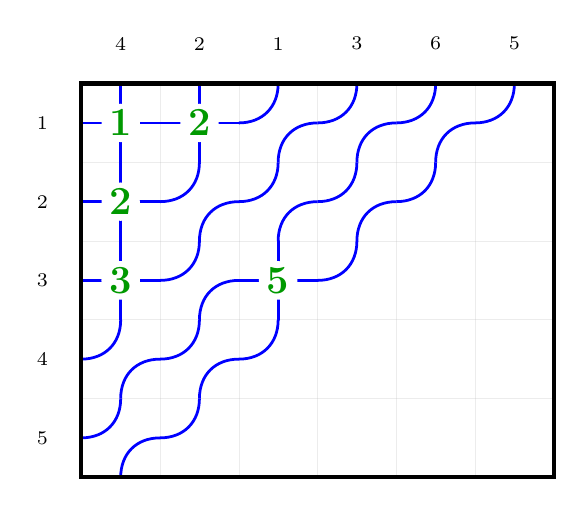
\begin{tikzpicture}[scale=1.0]
  \draw[lightgray, very thin, opacity=0.3] (0,1) -- (6,1);
  \draw[lightgray, very thin, opacity=0.3] (0,2) -- (6,2);
  \draw[lightgray, very thin, opacity=0.3] (0,3) -- (6,3);
  \draw[lightgray, very thin, opacity=0.3] (0,4) -- (6,4);
  \draw[lightgray, very thin, opacity=0.3] (0,5) -- (6,5);
  \draw[lightgray, very thin, opacity=0.3] (0,6) -- (6,6);
  \draw[lightgray, very thin, opacity=0.3] (0,1) -- (0,6);
  \draw[lightgray, very thin, opacity=0.3] (1,1) -- (1,6);
  \draw[lightgray, very thin, opacity=0.3] (2,1) -- (2,6);
  \draw[lightgray, very thin, opacity=0.3] (3,1) -- (3,6);
  \draw[lightgray, very thin, opacity=0.3] (4,1) -- (4,6);
  \draw[lightgray, very thin, opacity=0.3] (5,1) -- (5,6);
  \draw[lightgray, very thin, opacity=0.3] (6,1) -- (6,6);
  \draw[blue, line width=1.0pt, line cap=round] (0,5.5) -- (1,5.5);
  \draw[blue, line width=1.0pt, line cap=round] (0.5,5) -- (0.5,6);
  \draw[blue, line width=1.0pt, line cap=round] (1,5.5) -- (2,5.5);
  \draw[blue, line width=1.0pt, line cap=round] (1.5,5) -- (1.5,6);
  \draw[blue, line width=1.0pt] (2,5.5) .. controls (2.3,5.5) and (2.5,5.7) .. (2.5,6);
  \draw[blue, line width=1.0pt] (2.5,5) .. controls (2.5,5.3) and (2.7,5.5) .. (3,5.5);
  \draw[blue, line width=1.0pt] (3,5.5) .. controls (3.3,5.5) and (3.5,5.7) .. (3.5,6);
  \draw[blue, line width=1.0pt] (3.5,5) .. controls (3.5,5.3) and (3.7,5.5) .. (4,5.5);
  \draw[blue, line width=1.0pt] (4,5.5) .. controls (4.3,5.5) and (4.5,5.7) .. (4.5,6);
  \draw[blue, line width=1.0pt] (4.5,5) .. controls (4.5,5.3) and (4.7,5.5) .. (5,5.5);
  \draw[blue, line width=1.0pt] (5,5.5) .. controls (5.3,5.5) and (5.5,5.7) .. (5.5,6);
  \draw[blue, line width=1.0pt, line cap=round] (0,4.5) -- (1,4.5);
  \draw[blue, line width=1.0pt, line cap=round] (0.5,4) -- (0.5,5);
  \draw[blue, line width=1.0pt] (1,4.5) .. controls (1.3,4.5) and (1.5,4.7) .. (1.5,5);
  \draw[blue, line width=1.0pt] (1.5,4) .. controls (1.5,4.3) and (1.7,4.5) .. (2,4.5);
  \draw[blue, line width=1.0pt] (2,4.5) .. controls (2.3,4.5) and (2.5,4.7) .. (2.5,5);
  \draw[blue, line width=1.0pt] (2.5,4) .. controls (2.5,4.3) and (2.7,4.5) .. (3,4.5);
  \draw[blue, line width=1.0pt] (3,4.5) .. controls (3.3,4.5) and (3.5,4.7) .. (3.5,5);
  \draw[blue, line width=1.0pt] (3.5,4) .. controls (3.5,4.3) and (3.7,4.5) .. (4,4.5);
  \draw[blue, line width=1.0pt] (4,4.5) .. controls (4.3,4.5) and (4.5,4.7) .. (4.5,5);
  \draw[blue, line width=1.0pt, line cap=round] (0,3.5) -- (1,3.5);
  \draw[blue, line width=1.0pt, line cap=round] (0.5,3) -- (0.5,4);
  \draw[blue, line width=1.0pt] (1,3.5) .. controls (1.3,3.5) and (1.5,3.7) .. (1.5,4);
  \draw[blue, line width=1.0pt] (1.5,3) .. controls (1.5,3.3) and (1.7,3.5) .. (2,3.5);
  \draw[blue, line width=1.0pt, line cap=round] (2,3.5) -- (3,3.5);
  \draw[blue, line width=1.0pt, line cap=round] (2.5,3) -- (2.5,4);
  \draw[blue, line width=1.0pt] (3,3.5) .. controls (3.3,3.5) and (3.5,3.7) .. (3.5,4);
  \draw[blue, line width=1.0pt] (0,2.5) .. controls (0.3,2.5) and (0.5,2.7) .. (0.5,3);
  \draw[blue, line width=1.0pt] (0.5,2) .. controls (0.5,2.3) and (0.7,2.5) .. (1,2.5);
  \draw[blue, line width=1.0pt] (1,2.5) .. controls (1.3,2.5) and (1.5,2.7) .. (1.5,3);
  \draw[blue, line width=1.0pt] (1.5,2) .. controls (1.5,2.3) and (1.7,2.5) .. (2,2.5);
  \draw[blue, line width=1.0pt] (2,2.5) .. controls (2.3,2.5) and (2.5,2.7) .. (2.5,3);
  \draw[blue, line width=1.0pt] (0,1.5) .. controls (0.3,1.5) and (0.5,1.7) .. (0.5,2);
  \draw[blue, line width=1.0pt] (0.5,1) .. controls (0.5,1.3) and (0.7,1.5) .. (1,1.5);
  \draw[blue, line width=1.0pt] (1,1.5) .. controls (1.3,1.5) and (1.5,1.7) .. (1.5,2);
  \node[font=\Large\bfseries, text=green!60!black, fill=white, inner sep=0.5pt, circle, transform shape] at (1.5,5.5) {2};
  \node[font=\Large\bfseries, text=green!60!black, fill=white, inner sep=0.5pt, circle, transform shape] at (0.5,4.5) {2};
  \node[font=\Large\bfseries, text=green!60!black, fill=white, inner sep=0.5pt, circle, transform shape] at (0.5,3.5) {3};
  \node[font=\Large\bfseries, text=green!60!black, fill=white, inner sep=0.5pt, circle, transform shape] at (0.5,5.5) {1};
  \node[font=\Large\bfseries, text=green!60!black, fill=white, inner sep=0.5pt, circle, transform shape] at (2.5,3.5) {5};
  \node[font=\scriptsize, text=black, anchor=south] at (0.5,6.3) {4};
  \node[font=\scriptsize, text=black, anchor=south] at (1.5,6.3) {2};
  \node[font=\scriptsize, text=black, anchor=south] at (2.5,6.3) {1};
  \node[font=\scriptsize, text=black, anchor=south] at (3.5,6.3) {3};
  \node[font=\scriptsize, text=black, anchor=south] at (4.5,6.3) {6};
  \node[font=\scriptsize, text=black, anchor=south] at (5.5,6.3) {5};
  \node[font=\scriptsize, text=black, anchor=east] at (-0.3,5.5) {1};
  \node[font=\scriptsize, text=black, anchor=east] at (-0.3,4.5) {2};
  \node[font=\scriptsize, text=black, anchor=east] at (-0.3,3.5) {3};
  \node[font=\scriptsize, text=black, anchor=east] at (-0.3,2.5) {4};
  \node[font=\scriptsize, text=black, anchor=east] at (-0.3,1.5) {5};
  \draw[black, line width=1.5pt] (0,1) rectangle (6,6);
\end{tikzpicture}
\end{figure}


The main benefit of this is that visualizing $\rtt_R(i,j)$ is easy. The pipes that pass through position $(i,j)$ are labeled $s$ and $q$ for some $s,q>0$. For a positive root in an unoccupied square, we will have the following labeling, where $q<s$:

\begin{center}
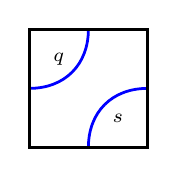
\begin{tikzpicture}[scale=1.5]
  % Draw the grid for a single square
  \draw[lightgray, very thin, opacity=0.3] (0,0) -- (1,0);
  \draw[lightgray, very thin, opacity=0.3] (0,1) -- (1,1);
  \draw[lightgray, very thin, opacity=0.3] (0,0) -- (0,1);
  \draw[lightgray, very thin, opacity=0.3] (1,0) -- (1,1);
  
  % Draw the elbow with two arcs
  % Blue arc (from left to top)
  \draw[blue, line width=1.0pt] (0,0.5) .. controls (0.3,0.5) and (0.5,0.7) .. (0.5,1);
  
  % Red arc (from bottom to right)
  \draw[blue, line width=1.0pt] (0.5,0) .. controls (0.5,0.3) and (0.7,0.5) .. (1,0.5);
  
  % Labels
  \node[font=\scriptsize, text=black] at (0.25,0.75) {$q$};
  \node[font=\scriptsize, text=black] at (0.75,0.25) {$s$};
  
  % Box around the grid
  \draw[black, line width=1.2pt] (0,0) rectangle (1,1);
\end{tikzpicture}
\end{center}

We observe that in the above RC graph, the position $(1,5)$ does not have this configuration. Placing a crossing there would create a negative root, and the pipes would cross twice. \emph{Note that this results in a collection of ordered pairs that is not an RC graph, if such a crossing exists.} For a valid RC graphs, only positive roots occur as crossings, and this happens if and only if pipes cross at most once.

\begin{figure}[h]
\centering
\caption{An invalid set of crossings causing pipes to cross more than once, caused by inserting a crossing at a negative root}
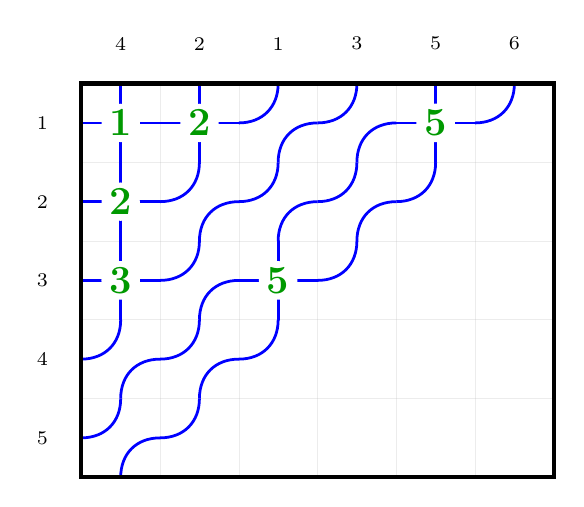
\begin{tikzpicture}[scale=1.0]
  \draw[lightgray, very thin, opacity=0.3] (0,1) -- (6,1);
  \draw[lightgray, very thin, opacity=0.3] (0,2) -- (6,2);
  \draw[lightgray, very thin, opacity=0.3] (0,3) -- (6,3);
  \draw[lightgray, very thin, opacity=0.3] (0,4) -- (6,4);
  \draw[lightgray, very thin, opacity=0.3] (0,5) -- (6,5);
  \draw[lightgray, very thin, opacity=0.3] (0,6) -- (6,6);
  \draw[lightgray, very thin, opacity=0.3] (0,1) -- (0,6);
  \draw[lightgray, very thin, opacity=0.3] (1,1) -- (1,6);
  \draw[lightgray, very thin, opacity=0.3] (2,1) -- (2,6);
  \draw[lightgray, very thin, opacity=0.3] (3,1) -- (3,6);
  \draw[lightgray, very thin, opacity=0.3] (4,1) -- (4,6);
  \draw[lightgray, very thin, opacity=0.3] (5,1) -- (5,6);
  \draw[lightgray, very thin, opacity=0.3] (6,1) -- (6,6);
  \draw[blue, line width=1.0pt, line cap=round] (0,5.5) -- (1,5.5);
  \draw[blue, line width=1.0pt, line cap=round] (0.5,5) -- (0.5,6);
  \draw[blue, line width=1.0pt, line cap=round] (1,5.5) -- (2,5.5);
  \draw[blue, line width=1.0pt, line cap=round] (1.5,5) -- (1.5,6);
  \draw[blue, line width=1.0pt] (2,5.5) .. controls (2.3,5.5) and (2.5,5.7) .. (2.5,6);
  \draw[blue, line width=1.0pt] (2.5,5) .. controls (2.5,5.3) and (2.7,5.5) .. (3,5.5);
  \draw[blue, line width=1.0pt] (3,5.5) .. controls (3.3,5.5) and (3.5,5.7) .. (3.5,6);
  \draw[blue, line width=1.0pt] (3.5,5) .. controls (3.5,5.3) and (3.7,5.5) .. (4,5.5);
  \draw[blue, line width=1.0pt, line cap=round] (4,5.5) -- (5,5.5);
  \draw[blue, line width=1.0pt, line cap=round] (4.5,5) -- (4.5,6);
  \draw[blue, line width=1.0pt] (5,5.5) .. controls (5.3,5.5) and (5.5,5.7) .. (5.5,6);
  \draw[blue, line width=1.0pt, line cap=round] (0,4.5) -- (1,4.5);
  \draw[blue, line width=1.0pt, line cap=round] (0.5,4) -- (0.5,5);
  \draw[blue, line width=1.0pt] (1,4.5) .. controls (1.3,4.5) and (1.5,4.7) .. (1.5,5);
  \draw[blue, line width=1.0pt] (1.5,4) .. controls (1.5,4.3) and (1.7,4.5) .. (2,4.5);
  \draw[blue, line width=1.0pt] (2,4.5) .. controls (2.3,4.5) and (2.5,4.7) .. (2.5,5);
  \draw[blue, line width=1.0pt] (2.5,4) .. controls (2.5,4.3) and (2.7,4.5) .. (3,4.5);
  \draw[blue, line width=1.0pt] (3,4.5) .. controls (3.3,4.5) and (3.5,4.7) .. (3.5,5);
  \draw[blue, line width=1.0pt] (3.5,4) .. controls (3.5,4.3) and (3.7,4.5) .. (4,4.5);
  \draw[blue, line width=1.0pt] (4,4.5) .. controls (4.3,4.5) and (4.5,4.7) .. (4.5,5);
  \draw[blue, line width=1.0pt, line cap=round] (0,3.5) -- (1,3.5);
  \draw[blue, line width=1.0pt, line cap=round] (0.5,3) -- (0.5,4);
  \draw[blue, line width=1.0pt] (1,3.5) .. controls (1.3,3.5) and (1.5,3.7) .. (1.5,4);
  \draw[blue, line width=1.0pt] (1.5,3) .. controls (1.5,3.3) and (1.7,3.5) .. (2,3.5);
  \draw[blue, line width=1.0pt, line cap=round] (2,3.5) -- (3,3.5);
  \draw[blue, line width=1.0pt, line cap=round] (2.5,3) -- (2.5,4);
  \draw[blue, line width=1.0pt] (3,3.5) .. controls (3.3,3.5) and (3.5,3.7) .. (3.5,4);
  \draw[blue, line width=1.0pt] (0,2.5) .. controls (0.3,2.5) and (0.5,2.7) .. (0.5,3);
  \draw[blue, line width=1.0pt] (0.5,2) .. controls (0.5,2.3) and (0.7,2.5) .. (1,2.5);
  \draw[blue, line width=1.0pt] (1,2.5) .. controls (1.3,2.5) and (1.5,2.7) .. (1.5,3);
  \draw[blue, line width=1.0pt] (1.5,2) .. controls (1.5,2.3) and (1.7,2.5) .. (2,2.5);
  \draw[blue, line width=1.0pt] (2,2.5) .. controls (2.3,2.5) and (2.5,2.7) .. (2.5,3);
  \draw[blue, line width=1.0pt] (0,1.5) .. controls (0.3,1.5) and (0.5,1.7) .. (0.5,2);
  \draw[blue, line width=1.0pt] (0.5,1) .. controls (0.5,1.3) and (0.7,1.5) .. (1,1.5);
  \draw[blue, line width=1.0pt] (1,1.5) .. controls (1.3,1.5) and (1.5,1.7) .. (1.5,2);
  \node[font=\Large\bfseries, text=green!60!black, fill=white, inner sep=0.5pt, circle, transform shape] at (1.5,5.5) {2};
  \node[font=\Large\bfseries, text=green!60!black, fill=white, inner sep=0.5pt, circle, transform shape] at (0.5,4.5) {2};
  \node[font=\Large\bfseries, text=green!60!black, fill=white, inner sep=0.5pt, circle, transform shape] at (4.5,5.5) {5};
  \node[font=\Large\bfseries, text=green!60!black, fill=white, inner sep=0.5pt, circle, transform shape] at (0.5,3.5) {3};
  \node[font=\Large\bfseries, text=green!60!black, fill=white, inner sep=0.5pt, circle, transform shape] at (0.5,5.5) {1};
  \node[font=\Large\bfseries, text=green!60!black, fill=white, inner sep=0.5pt, circle, transform shape] at (2.5,3.5) {5};
  \node[font=\scriptsize, text=black, anchor=south] at (0.5,6.3) {4};
  \node[font=\scriptsize, text=black, anchor=south] at (1.5,6.3) {2};
  \node[font=\scriptsize, text=black, anchor=south] at (2.5,6.3) {1};
  \node[font=\scriptsize, text=black, anchor=south] at (3.5,6.3) {3};
  \node[font=\scriptsize, text=black, anchor=south] at (4.5,6.3) {5};
  \node[font=\scriptsize, text=black, anchor=south] at (5.5,6.3) {6};
  \node[font=\scriptsize, text=black, anchor=east] at (-0.3,5.5) {1};
  \node[font=\scriptsize, text=black, anchor=east] at (-0.3,4.5) {2};
  \node[font=\scriptsize, text=black, anchor=east] at (-0.3,3.5) {3};
  \node[font=\scriptsize, text=black, anchor=east] at (-0.3,2.5) {4};
  \node[font=\scriptsize, text=black, anchor=east] at (-0.3,1.5) {5};
  \draw[black, line width=1.5pt] (0,1) rectangle (6,6);
\end{tikzpicture}
\end{figure}

\subsection{Zeroing out the last row}

We proceed now to define a product on $\BRC$ turning it into a ring. To do this, we need to be able to define a function $\zeromap:\BRC\to\BRC$ trimming empty rows from the bottom instead of from the top. This is far more complicated.


\newcommand{\xleadsto}[2][]{\overset{#2}{\leadsto}}

\newcommand{\ins}[2]{{#2\xleadsto{#1}}}

\begin{algorithm}
\caption{Basic monk insertion $\ins{k}{i} R$}
\label{algorithm:monk}
\begin{algorithmic}[1]
		\State \textbf{Input:} An RC graph $R$, parameter $k$, and an integer $i$ with $1\leq i\leq k$.
		\State \textbf{Output:} A modified RC graph $R'$ with $\wtt_j(R')=\wtt_j(R)$  for $j\neq i$ and $\wtt_i(R')=\wtt_i(R)+1$ such that $\wof{R}\tom{k} \wof{R'}$.
		\State Find leftmost position $(i, j) \notin R$ in row $i$ such that if $\rtt_R(i, j)=(a,b)$, then $a\leq k < b$.
		\State $R \gets R \cup \{(i, j)\}$
    \If{there exists $(i', j') \in R$ with $\rtt_R(i', j') \in \Phi^-$}
        \State $R \gets R \setminus \{(i', j')\}$
        \State Return to step 3 substituting $i = i'$.
    \EndIf
		\State \Return $R$
	\end{algorithmic}
\end{algorithm}

\begin{algorithm} 
	\caption{Pseudo-Pieri insertion $\ins{k}{I} R$}
	\label{algorithm:insertion}
	\begin{algorithmic}[1]
		\State \textbf{Input:} An RC graph $R$, parameter $k$, and sequence $I = \{i_1, \ldots, i_m\}$ with $k\geq i_1 \geq i_2 \geq \cdots \geq i_m \geq 1$.
		\State \textbf{Output:} A modified RC graph $R'$ with $\wtt_i(R')=\wtt_i(R)$ for $i\notin I$ and $\wtt_i(R')=\wtt_i(R)+\#\{j \mid i_j = i\}$ for $i\in I$ such that $\wof{R}\Tom{k} \wof{R'}$.
		\State \textbf{Initialize:} Let $L \gets [\,]$ (empty list of pairs $(a, b)$ where $a \leq k < b$), and $U\gets [\,]$ (empty list of positions).
		\For{each $i \in (i_1, \ldots, i_m)$}
		\State Find leftmost position $(i, j) \notin R$ in row $i$ satisfying $j>j'$ for all $(i,j')\in U$ such that either:
		\State \quad a) $\rtt_R(i, j) = (s, q)$ where $s \leq k < q$ and $q \notin \{b \mid (a, b) \in L\}$.
		\State \quad b) $\rtt_R(i, j) = (b_r, q)$ where $q > k$, $b_r<q$, and $q \notin \{b \mid (a, b) \in L\}$.
		\State $R \gets R \cup \{(i, j)\}$ and $U\gets U \cup \{(i, j)\}$
		\State Update $L$ by adding $(s, q)$ or replacing $(a_r, b_r)$ with $(a_r, q)$ and $(a_r, b_r)$.
		\If{there exists $(i', j') \in R$ with $\rtt_R(i', j') \in \Phi^-$}
        
    \State $R \gets R \setminus \{(i', j')\}$
		\State Let $\rtt_R(i', j') = (q, s)$
		\If{$(s, q) \in L$}
		\State Remove $(s, q)$ from $L$
		\Else
		\State Remove $(a_r, q)$ from $L$, where $(a_r, q),(a_r,s)\in L$
		\EndIf
		\State Return to step 5 to insert $i'$.
    \EndIf
		\EndFor
		\State \Return $R$
	\end{algorithmic}
\end{algorithm}


\begin{algorithm} 
	\caption{Map $\zeromap(R)$ zeroing out last row}
	\label{algorithm:zero}
	\begin{algorithmic}[1]
		\State \textbf{Input:} A bounded RC graph $R$ with $\hr(R)=n$ and row $n$ empty.
		\State \textbf{Output:} A bounded RC graph $R'$ with $\hr(R')=n-1$, $|R'|=|R|$ (same number of crossings), and $\wof{R}\downvar{n} \wof{R'}$.
		
		\If{$R$ with last row removed is a valid bounded RC graph}
		\State \Return $R$ with last row removed
		\Else
		\State Let $R_0 \gets R$.
		\State Find the maximal $p$ and sequence $\{(i_m, j_m)\}_{m=1}^p$ such that:
		\State \quad $\rtt_{R_{m-1}}(i_m, j_m) = (n+m-1,n+m)$ for each $m$, where $R_m = R_{m-1}\setminus\{(i_m, j_m)\}$ for each $m\geq 1$.
		\State $R^- \gets R \setminus \{(i_1, j_1), \ldots, (i_p, j_p)\}$.
		\State Let $I \gets (i_1, i_2, \ldots, i_p)$.
		\State $D \gets R^- \cup \{(n, 1), (n, 2), \ldots, (n, p)\}$.
		\State $D' \gets \ins{n-1}{I} D$
		\State $R' \gets \{(i, j) \in D' \mid i < n\}$ as a bounded RC graph with $n-1$ rows.
		\State \Return $R'$.
		\EndIf
	\end{algorithmic}
\end{algorithm}

See Figure \ref{fig:zeroing} for an example of the zeroing operation (Algorithm \ref{algorithm:zero}). 

\def\multiset#1#2{\ensuremath{\left(\kern-.3em\left(\genfrac{}{}{0pt}{}{#1}{#2}\right)\kern-.3em\right)}}


Note that Algorithm \ref{algorithm:insertion} is \emph{not} a realization of Sottile's Pieri formula for complete symmetric polynomials, despite preserving the relevant Bruhat relation. This is because the map 
$$\multiset{k}{p}\times\RC(w)\to \RC(n)$$
given by 
$$(I, R)\mapsto \ins{k}{I} R$$ 
need not be injective.

\begin{definition}\label{definition:zeromap}
Let $R$ be an RC graph with $\hr(R) = n$ such that row $n$ is empty. We define $\zeromap(R)$ to be the output of Algorithm \ref{algorithm:zero}, an RC graph with $n-1$ rows, on input $R$.
\end{definition}

\begin{figure}[htbp]
\centering

% First diagram
\begin{minipage}{0.45\textwidth}
\centering
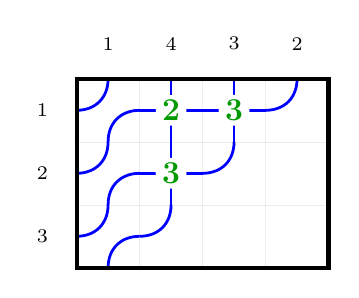
\begin{tikzpicture}[scale=0.8]
  \draw[lightgray, very thin, opacity=0.3] (0,1) -- (4,1);
  \draw[lightgray, very thin, opacity=0.3] (0,2) -- (4,2);
  \draw[lightgray, very thin, opacity=0.3] (0,3) -- (4,3);
  \draw[lightgray, very thin, opacity=0.3] (0,4) -- (4,4);
  \draw[lightgray, very thin, opacity=0.3] (0,1) -- (0,4);
  \draw[lightgray, very thin, opacity=0.3] (1,1) -- (1,4);
  \draw[lightgray, very thin, opacity=0.3] (2,1) -- (2,4);
  \draw[lightgray, very thin, opacity=0.3] (3,1) -- (3,4);
  \draw[lightgray, very thin, opacity=0.3] (4,1) -- (4,4);
  \draw[blue, line width=1.0pt] (0,3.5) .. controls (0.3,3.5) and (0.5,3.7) .. (0.5,4);
  \draw[blue, line width=1.0pt] (0.5,3) .. controls (0.5,3.3) and (0.7,3.5) .. (1,3.5);
  \draw[blue, line width=1.0pt, line cap=round] (1,3.5) -- (2,3.5);
  \draw[blue, line width=1.0pt, line cap=round] (1.5,3) -- (1.5,4);
  \draw[blue, line width=1.0pt, line cap=round] (2,3.5) -- (3,3.5);
  \draw[blue, line width=1.0pt, line cap=round] (2.5,3) -- (2.5,4);
  \draw[blue, line width=1.0pt] (3,3.5) .. controls (3.3,3.5) and (3.5,3.7) .. (3.5,4);
  \draw[blue, line width=1.0pt] (0,2.5) .. controls (0.3,2.5) and (0.5,2.7) .. (0.5,3);
  \draw[blue, line width=1.0pt] (0.5,2) .. controls (0.5,2.3) and (0.7,2.5) .. (1,2.5);
  \draw[blue, line width=1.0pt, line cap=round] (1,2.5) -- (2,2.5);
  \draw[blue, line width=1.0pt, line cap=round] (1.5,2) -- (1.5,3);
  \draw[blue, line width=1.0pt] (2,2.5) .. controls (2.3,2.5) and (2.5,2.7) .. (2.5,3);
  \draw[blue, line width=1.0pt] (0,1.5) .. controls (0.3,1.5) and (0.5,1.7) .. (0.5,2);
  \draw[blue, line width=1.0pt] (0.5,1) .. controls (0.5,1.3) and (0.7,1.5) .. (1,1.5);
  \draw[blue, line width=1.0pt] (1,1.5) .. controls (1.3,1.5) and (1.5,1.7) .. (1.5,2);
  \node[font=\Large\bfseries, text=green!60!black, fill=white, inner sep=0.5pt, circle, transform shape] at (1.5,3.5) {2};
  \node[font=\Large\bfseries, text=green!60!black, fill=white, inner sep=0.5pt, circle, transform shape] at (2.5,3.5) {3};
  \node[font=\Large\bfseries, text=green!60!black, fill=white, inner sep=0.5pt, circle, transform shape] at (1.5,2.5) {3};
  \node[font=\scriptsize, text=black, anchor=south] at (0.5,4.3) {1};
  \node[font=\scriptsize, text=black, anchor=south] at (1.5,4.3) {4};
  \node[font=\scriptsize, text=black, anchor=south] at (2.5,4.3) {3};
  \node[font=\scriptsize, text=black, anchor=south] at (3.5,4.3) {2};
  \node[font=\scriptsize, text=black, anchor=east] at (-0.3,3.5) {1};
  \node[font=\scriptsize, text=black, anchor=east] at (-0.3,2.5) {2};
  \node[font=\scriptsize, text=black, anchor=east] at (-0.3,1.5) {3};
  \draw[black, line width=1.5pt] (0,1) rectangle (4,4);
\end{tikzpicture}
\caption*{(a) Initial RC graph $R$}
\end{minipage}
\hfill
% Second diagram
\begin{minipage}{0.45\textwidth}
\centering
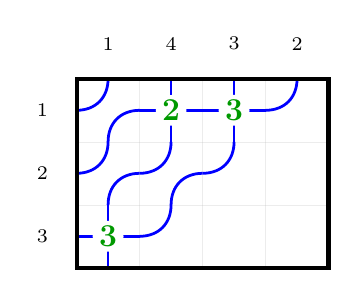
\begin{tikzpicture}[scale=0.8]
  \draw[lightgray, very thin, opacity=0.3] (0,1) -- (4,1);
  \draw[lightgray, very thin, opacity=0.3] (0,2) -- (4,2);
  \draw[lightgray, very thin, opacity=0.3] (0,3) -- (4,3);
  \draw[lightgray, very thin, opacity=0.3] (0,4) -- (4,4);
  \draw[lightgray, very thin, opacity=0.3] (0,1) -- (0,4);
  \draw[lightgray, very thin, opacity=0.3] (1,1) -- (1,4);
  \draw[lightgray, very thin, opacity=0.3] (2,1) -- (2,4);
  \draw[lightgray, very thin, opacity=0.3] (3,1) -- (3,4);
  \draw[lightgray, very thin, opacity=0.3] (4,1) -- (4,4);
  \draw[blue, line width=1.0pt] (0,3.5) .. controls (0.3,3.5) and (0.5,3.7) .. (0.5,4);
  \draw[blue, line width=1.0pt] (0.5,3) .. controls (0.5,3.3) and (0.7,3.5) .. (1,3.5);
  \draw[blue, line width=1.0pt, line cap=round] (1,3.5) -- (2,3.5);
  \draw[blue, line width=1.0pt, line cap=round] (1.5,3) -- (1.5,4);
  \draw[blue, line width=1.0pt, line cap=round] (2,3.5) -- (3,3.5);
  \draw[blue, line width=1.0pt, line cap=round] (2.5,3) -- (2.5,4);
  \draw[blue, line width=1.0pt] (3,3.5) .. controls (3.3,3.5) and (3.5,3.7) .. (3.5,4);
  \draw[blue, line width=1.0pt] (0,2.5) .. controls (0.3,2.5) and (0.5,2.7) .. (0.5,3);
  \draw[blue, line width=1.0pt] (0.5,2) .. controls (0.5,2.3) and (0.7,2.5) .. (1,2.5);
  \draw[blue, line width=1.0pt] (1,2.5) .. controls (1.3,2.5) and (1.5,2.7) .. (1.5,3);
  \draw[blue, line width=1.0pt] (1.5,2) .. controls (1.5,2.3) and (1.7,2.5) .. (2,2.5);
  \draw[blue, line width=1.0pt] (2,2.5) .. controls (2.3,2.5) and (2.5,2.7) .. (2.5,3);
  \draw[blue, line width=1.0pt, line cap=round] (0,1.5) -- (1,1.5);
  \draw[blue, line width=1.0pt, line cap=round] (0.5,1) -- (0.5,2);
  \draw[blue, line width=1.0pt] (1,1.5) .. controls (1.3,1.5) and (1.5,1.7) .. (1.5,2);
  \node[font=\Large\bfseries, text=green!60!black, fill=white, inner sep=0.5pt, circle, transform shape] at (0.5,1.5) {3};
  \node[font=\Large\bfseries, text=green!60!black, fill=white, inner sep=0.5pt, circle, transform shape] at (1.5,3.5) {2};
  \node[font=\Large\bfseries, text=green!60!black, fill=white, inner sep=0.5pt, circle, transform shape] at (2.5,3.5) {3};
  \node[font=\scriptsize, text=black, anchor=south] at (0.5,4.3) {1};
  \node[font=\scriptsize, text=black, anchor=south] at (1.5,4.3) {4};
  \node[font=\scriptsize, text=black, anchor=south] at (2.5,4.3) {3};
  \node[font=\scriptsize, text=black, anchor=south] at (3.5,4.3) {2};
  \node[font=\scriptsize, text=black, anchor=east] at (-0.3,3.5) {1};
  \node[font=\scriptsize, text=black, anchor=east] at (-0.3,2.5) {2};
  \node[font=\scriptsize, text=black, anchor=east] at (-0.3,1.5) {3};
  \draw[black, line width=1.5pt] (0,1) rectangle (4,4);
\end{tikzpicture}
\caption*{(b) After deleting $(2,2)$ with $\rtt_R(2,2)=\alpha_3$ and moving to row $3$}
\end{minipage}

\vspace{1em}

% Third diagram
\begin{minipage}{0.45\textwidth}
\centering
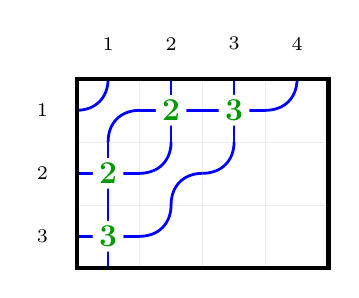
\begin{tikzpicture}[scale=0.8]
  \draw[lightgray, very thin, opacity=0.3] (0,1) -- (4,1);
  \draw[lightgray, very thin, opacity=0.3] (0,2) -- (4,2);
  \draw[lightgray, very thin, opacity=0.3] (0,3) -- (4,3);
  \draw[lightgray, very thin, opacity=0.3] (0,4) -- (4,4);
  \draw[lightgray, very thin, opacity=0.3] (0,1) -- (0,4);
  \draw[lightgray, very thin, opacity=0.3] (1,1) -- (1,4);
  \draw[lightgray, very thin, opacity=0.3] (2,1) -- (2,4);
  \draw[lightgray, very thin, opacity=0.3] (3,1) -- (3,4);
  \draw[lightgray, very thin, opacity=0.3] (4,1) -- (4,4);
  \draw[blue, line width=1.0pt] (0,3.5) .. controls (0.3,3.5) and (0.5,3.7) .. (0.5,4);
  \draw[blue, line width=1.0pt] (0.5,3) .. controls (0.5,3.3) and (0.7,3.5) .. (1,3.5);
  \draw[blue, line width=1.0pt, line cap=round] (1,3.5) -- (2,3.5);
  \draw[blue, line width=1.0pt, line cap=round] (1.5,3) -- (1.5,4);
  \draw[blue, line width=1.0pt, line cap=round] (2,3.5) -- (3,3.5);
  \draw[blue, line width=1.0pt, line cap=round] (2.5,3) -- (2.5,4);
  \draw[blue, line width=1.0pt] (3,3.5) .. controls (3.3,3.5) and (3.5,3.7) .. (3.5,4);
  \draw[blue, line width=1.0pt, line cap=round] (0,2.5) -- (1,2.5);
  \draw[blue, line width=1.0pt, line cap=round] (0.5,2) -- (0.5,3);
  \draw[blue, line width=1.0pt] (1,2.5) .. controls (1.3,2.5) and (1.5,2.7) .. (1.5,3);
  \draw[blue, line width=1.0pt] (1.5,2) .. controls (1.5,2.3) and (1.7,2.5) .. (2,2.5);
  \draw[blue, line width=1.0pt] (2,2.5) .. controls (2.3,2.5) and (2.5,2.7) .. (2.5,3);
  \draw[blue, line width=1.0pt, line cap=round] (0,1.5) -- (1,1.5);
  \draw[blue, line width=1.0pt, line cap=round] (0.5,1) -- (0.5,2);
  \draw[blue, line width=1.0pt] (1,1.5) .. controls (1.3,1.5) and (1.5,1.7) .. (1.5,2);
  \node[font=\Large\bfseries, text=green!60!black, fill=white, inner sep=0.5pt, circle, transform shape] at (0.5,1.5) {3};
  \node[font=\Large\bfseries, text=green!60!black, fill=white, inner sep=0.5pt, circle, transform shape] at (1.5,3.5) {2};
  \node[font=\Large\bfseries, text=green!60!black, fill=white, inner sep=0.5pt, circle, transform shape] at (2.5,3.5) {3};
  \node[font=\Large\bfseries, text=green!60!black, fill=white, inner sep=0.5pt, circle, transform shape] at (0.5,2.5) {2};
  \node[font=\scriptsize, text=black, anchor=south] at (0.5,4.3) {1};
  \node[font=\scriptsize, text=black, anchor=south] at (1.5,4.3) {2};
  \node[font=\scriptsize, text=black, anchor=south] at (2.5,4.3) {3};
  \node[font=\scriptsize, text=black, anchor=south] at (3.5,4.3) {4};
  \node[font=\scriptsize, text=black, anchor=east] at (-0.3,3.5) {1};
  \node[font=\scriptsize, text=black, anchor=east] at (-0.3,2.5) {2};
  \node[font=\scriptsize, text=black, anchor=east] at (-0.3,1.5) {3};
  \draw[black, line width=1.5pt] (0,1) rectangle (4,4);
\end{tikzpicture}
\caption*{(c) After insertion with $i_1=2$}
\end{minipage}
\hfill
% Fourth diagram
\begin{minipage}{0.45\textwidth}
\centering
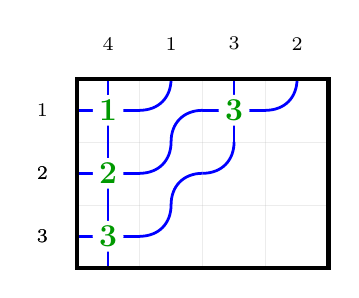
\begin{tikzpicture}[scale=0.8]
  \draw[lightgray, very thin, opacity=0.3] (0,1) -- (4,1);
  \draw[lightgray, very thin, opacity=0.3] (0,2) -- (4,2);
  \draw[lightgray, very thin, opacity=0.3] (0,3) -- (4,3);
  \draw[lightgray, very thin, opacity=0.3] (0,4) -- (4,4);
  \draw[lightgray, very thin, opacity=0.3] (0,1) -- (0,4);
  \draw[lightgray, very thin, opacity=0.3] (1,1) -- (1,4);
  \draw[lightgray, very thin, opacity=0.3] (2,1) -- (2,4);
  \draw[lightgray, very thin, opacity=0.3] (3,1) -- (3,4);
  \draw[lightgray, very thin, opacity=0.3] (4,1) -- (4,4);
  \draw[blue, line width=1.0pt, line cap=round] (0,3.5) -- (1,3.5);
  \draw[blue, line width=1.0pt, line cap=round] (0.5,3) -- (0.5,4);
  \draw[blue, line width=1.0pt] (1,3.5) .. controls (1.3,3.5) and (1.5,3.7) .. (1.5,4);
  \draw[blue, line width=1.0pt] (1.5,3) .. controls (1.5,3.3) and (1.7,3.5) .. (2,3.5);
  \draw[blue, line width=1.0pt, line cap=round] (2,3.5) -- (3,3.5);
  \draw[blue, line width=1.0pt, line cap=round] (2.5,3) -- (2.5,4);
  \draw[blue, line width=1.0pt] (3,3.5) .. controls (3.3,3.5) and (3.5,3.7) .. (3.5,4);
  \draw[blue, line width=1.0pt, line cap=round] (0,2.5) -- (1,2.5);
  \draw[blue, line width=1.0pt, line cap=round] (0.5,2) -- (0.5,3);
  \draw[blue, line width=1.0pt] (1,2.5) .. controls (1.3,2.5) and (1.5,2.7) .. (1.5,3);
  \draw[blue, line width=1.0pt] (1.5,2) .. controls (1.5,2.3) and (1.7,2.5) .. (2,2.5);
  \draw[blue, line width=1.0pt] (2,2.5) .. controls (2.3,2.5) and (2.5,2.7) .. (2.5,3);
  \draw[blue, line width=1.0pt, line cap=round] (0,1.5) -- (1,1.5);
  \draw[blue, line width=1.0pt, line cap=round] (0.5,1) -- (0.5,2);
  \draw[blue, line width=1.0pt] (1,1.5) .. controls (1.3,1.5) and (1.5,1.7) .. (1.5,2);
  \node[font=\Large\bfseries, text=green!60!black, fill=white, inner sep=0.5pt, circle, transform shape] at (0.5,1.5) {3};
  \node[font=\Large\bfseries, text=green!60!black, fill=white, inner sep=0.5pt, circle, transform shape] at (0.5,3.5) {1};
  \node[font=\Large\bfseries, text=green!60!black, fill=white, inner sep=0.5pt, circle, transform shape] at (2.5,3.5) {3};
  \node[font=\Large\bfseries, text=green!60!black, fill=white, inner sep=0.5pt, circle, transform shape] at (0.5,2.5) {2};
  \node[font=\scriptsize, text=black, anchor=south] at (0.5,4.3) {4};
  \node[font=\scriptsize, text=black, anchor=south] at (1.5,4.3) {1};
  \node[font=\scriptsize, text=black, anchor=south] at (2.5,4.3) {3};
  \node[font=\scriptsize, text=black, anchor=south] at (3.5,4.3) {2};
  \node[font=\scriptsize, text=black, anchor=east] at (-0.3,3.5) {1};
  \node[font=\scriptsize, text=black, anchor=east] at (-0.3,2.5) {2};
  \node[font=\scriptsize, text=black, anchor=east] at (-0.3,1.5) {3};
  \node[font=\scriptsize, text=black, anchor=east] at (-0.3,2.5) {2};
  \node[font=\scriptsize, text=black, anchor=east] at (-0.3,1.5) {3};
  \draw[black, line width=1.5pt] (0,1) rectangle (4,4);
\end{tikzpicture}
\caption*{(d) After rectification}
\end{minipage}

\vspace{1em}

% Fifth diagram
\begin{minipage}{0.45\textwidth}
\centering
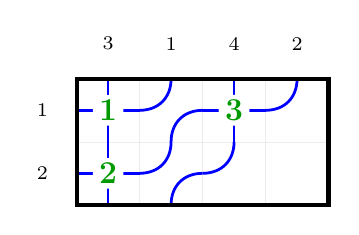
\begin{tikzpicture}[scale=0.8]
  \draw[lightgray, very thin, opacity=0.3] (0,2) -- (4,2);
  \draw[lightgray, very thin, opacity=0.3] (0,3) -- (4,3);
  \draw[lightgray, very thin, opacity=0.3] (0,4) -- (4,4);
  \draw[lightgray, very thin, opacity=0.3] (0,2) -- (0,4);
  \draw[lightgray, very thin, opacity=0.3] (1,2) -- (1,4);
  \draw[lightgray, very thin, opacity=0.3] (2,2) -- (2,4);
  \draw[lightgray, very thin, opacity=0.3] (3,2) -- (3,4);
  \draw[lightgray, very thin, opacity=0.3] (4,2) -- (4,4);
  \draw[blue, line width=1.0pt, line cap=round] (0,3.5) -- (1,3.5);
  \draw[blue, line width=1.0pt, line cap=round] (0.5,3) -- (0.5,4);
  \draw[blue, line width=1.0pt] (1,3.5) .. controls (1.3,3.5) and (1.5,3.7) .. (1.5,4);
  \draw[blue, line width=1.0pt] (1.5,3) .. controls (1.5,3.3) and (1.7,3.5) .. (2,3.5);
  \draw[blue, line width=1.0pt, line cap=round] (2,3.5) -- (3,3.5);
  \draw[blue, line width=1.0pt, line cap=round] (2.5,3) -- (2.5,4);
  \draw[blue, line width=1.0pt] (3,3.5) .. controls (3.3,3.5) and (3.5,3.7) .. (3.5,4);
  \draw[blue, line width=1.0pt, line cap=round] (0,2.5) -- (1,2.5);
  \draw[blue, line width=1.0pt, line cap=round] (0.5,2) -- (0.5,3);
  \draw[blue, line width=1.0pt] (1,2.5) .. controls (1.3,2.5) and (1.5,2.7) .. (1.5,3);
  \draw[blue, line width=1.0pt] (1.5,2) .. controls (1.5,2.3) and (1.7,2.5) .. (2,2.5);
  \draw[blue, line width=1.0pt] (2,2.5) .. controls (2.3,2.5) and (2.5,2.7) .. (2.5,3);
  \node[font=\Large\bfseries, text=green!60!black, fill=white, inner sep=0.5pt, circle, transform shape] at (0.5,3.5) {1};
  \node[font=\Large\bfseries, text=green!60!black, fill=white, inner sep=0.5pt, circle, transform shape] at (2.5,3.5) {3};
  \node[font=\Large\bfseries, text=green!60!black, fill=white, inner sep=0.5pt, circle, transform shape] at (0.5,2.5) {2};
  \node[font=\scriptsize, text=black, anchor=south] at (0.5,4.3) {3};
  \node[font=\scriptsize, text=black, anchor=south] at (1.5,4.3) {1};
  \node[font=\scriptsize, text=black, anchor=south] at (2.5,4.3) {4};
  \node[font=\scriptsize, text=black, anchor=south] at (3.5,4.3) {2};
  \node[font=\scriptsize, text=black, anchor=east] at (-0.3,3.5) {1};
  \node[font=\scriptsize, text=black, anchor=east] at (-0.3,2.5) {2};
  \draw[black, line width=1.5pt] (0,2) rectangle (4,4);
\end{tikzpicture}
\caption*{(e) Final result $\zeromap(R)=(R',2)$ after removing row 3}
\end{minipage}

\caption{Step-by-step computation of $\zeromap(R)$ for $R=\{(1,2),(1,3),(2,2)\}$.}
\label{fig:zeroing}
\end{figure}



\begin{lemma} \label{lemma:insertworks}
Given an RC graph $R$, an integer $k$, and $k\geq i_1\geq\cdots\geq i_m\geq 1$, Algorithm \ref{algorithm:insertion} produces a valid RC graph $R'$ satisfying
$$\wtt_i(R') = \wtt_i(R) + \#\{j \mid i_j = i\}$$
and
$$\wof{R}\Tom{k} \wof{R'}$$
\end{lemma}
\begin{proof}
Set $R_0=R$ to be the initial RC graph. We claim that given $R$ and $L$ at the start of iteration $p$ of the main loop, we have that $R$ is a valid RC graph satisfying
$$\wtt_i(R) = \wtt_i(R_0) + \#\{j \leq p-1 \mid i_j = i\}$$
and
$$\wof{R} = \wof{R_0}t_{a_1b_1}\cdots t_{a_{p-1}b_{p-1}}$$
where $L=[(a_1,b_1),\ldots,(a_p,b_p)]$. This is clear for $p=1$. For larger $p$, suppose we are inserting at row $i_p$. If we are in case (a) of Step 5, then adding $(i_p,j)$ to $R$ adds the root $t_s - t_q$ to the inversion set of $\wof{R}$, and multiplying by $t_{sq}$ gives the desired result. If we are in case (b) of Step 5, then adding $(i_p,j)$ to $R$ results in multiplication by $t_{b_rq}$. This commutes past the other reflections to meet $t_{a_rb_r}$. We thus have the situation
$$t_{a_rb_r}t_{b_rq} = t_{a_rq}t_{a_rb_r}$$
This ensures that the product remains as desired if the RC graph is valid. However, the condition that the RC graph $R$ be valid is not guaranteed after this step, so we must rectify. Suppose we must rectify at row $i - 1$. We find a negative root $(i-1, j')$ which must have been created by the insertion, and hence by the strong exchange property equal to $\rtt_R(i, j)$ that was inserted. Removing this root (from both the graph and from $L$) returns us to the original permutation at the beginning of the iteration, and performing the insert at row $i-1$ adds a new positive root, giving the desired result on the permutation. The weight is unchanged since we removed and added one crossing in row $i-1$. If the algorithm ends here, we have instead multiplied by the new reflection obtained in the ultimate insert step. Otherwise, repeating this process for all necessary rectifications completes the proof of the claim. The claim iterated to $p=m+1$ yields the desired result, and the method of updating $L$ ensures that the $b_j$ are all distinct, so that $\wof{R}\Tom{k} \wof{R'}$.
\end{proof}


\begin{lemma}
Given a bounded RC graph $R$ with $\hr(R)=n$ such that row $n$ is empty, Algorithm \ref{algorithm:zero} produces a valid bounded RC graph $R'$ with $\hr(R')=n-1$ satisfying
$$\wtt(R') = \wtt(R)$$
\end{lemma}
\begin{proof}
	Stripping out the crossings at roots $(n, n+1), (n+1, n+2), \ldots, (n + p - 1, n + p)$ removes exactly one crossing from each of rows $i_1, i_2, \ldots, i_p$, and moving them to the last row to obtain $R_1$ ensures that $\wof{R}=\wof{R_1}$. By construction, the portion of the RC graph in rows with index less than $n$ is valid (meaning its max descent is at most $n-1$). Applying Algorithm \ref{algorithm:insertion} to insert at rows $i_1, i_2, \ldots, i_p$ adds different crossings to preserve the number of elements in each row without adding descents past index $n$ in the permutation, by Lemma \ref{lemma:insertworks}. Removing row $n$ then yields a valid bounded RC graph $R'$ with $|R'|=n-1$ and the desired properties. 
\end{proof}



\begin{theorem} \label{theorem:zero_bijection}
Let $w$ be a permutation with last descent at most $n$. Let $\mathcal{RC}(w,n)^0$ be the set of bounded RC graphs $R$ with $\hr(R)=n$ such that $\wof{R}=w$ and row $n$ is empty. Then
$$\zeromap:\mathcal{RC}(w, n)^{0}\to \bigcup_{w\downvar{n} w'}\mathcal{RC}(w', n-1)$$
is a weight-preserving bijection.
\end{theorem}

To prove Theorem \ref{theorem:zero_bijection} for $n=2$, we may characterize the bounded RC graphs $R$ with $|R|=2$ such that row $2$ is empty and $\maxd(\wof{R})=2$ as those for permutations $w=s_k s_{k-1}\cdots s_2$ for some $k>1$. Algorithm \ref{algorithm:zero} in this case consists moves the entirety of the crossings in row $1$ to row $2$. The procedure then inserts $k-1$ crossings into row $1$ in order from left to right, which must have roots $t_q - t_s$ such that $q=1$. Thus $R'$ is precisely $\{(1,1), (1,2), (1,3), \ldots, (1, k-1)\}$, which is the unique bounded RC graph for the permutation $w' = s_{k-1} s_{k-2}\cdots s_1$ with one row. This establishes the base case.

For the induction step, we require the following lemmas.

\begin{lemma} \label{lemma:zerotransition}
Let $R$ be a bounded RC graph with $\hr(R)=n\geq 2$ such that row $n$ is empty. Then if $\zeromap(R) = R'$, we have
$$\wof{R}\downvar{n} \wof{R'}$$
\end{lemma}
\begin{proof}
Let $w=\wof{R}$ and suppose $\code_n(w) = m$. By construction, the second to last step of Algorithm \ref{algorithm:zero} yields a bounded RC graph $\widetilde{R}$ with $|\widetilde{R}|=n$ such that if $\widetilde{w} = \wof{\widetilde{R}}$, then
$$\widetilde{w}(n) > \widetilde{w}(n+1) < \widetilde{w}(n+2) < \cdots < \widetilde{w}(n + m)$$
and
$$w\Tom{n-1}\widetilde{w}$$
via reflections $t_{ab}$ such that $n\leq b\leq n+m$. Let $w' = \wof{R'}$. We also have
$$\widetilde{w}\Tom{n}\varphi_{n, N}(w')$$
via only reflections $t_{nb}$ such that $b>n+m$. We claim that
$$w\Tom{n} \varphi_{n, N}(w')$$
This can only fail if $\widetilde{w}(n)\neq w(n)$ by the observations above. However, the pipe labeled $n$, by virtue of the fact that we have $(n,1),\ldots,(n,m)$ populated, will always lie to the right of pipes $n+1,n+2,\ldots,n+m$ in the wiring diagram for $\widetilde{w}$ or any intermediate stage. Inserting into any row that contained a crossing $(n, n+p)$, there must be a valid empty space to the left of the pipe labeled $n$ since we have deleted these crossings. By virtue of the fact that the leftmost is always chosen, no reflection $(i,n)$ will ever be inserted. This ensures that $\widetilde{w}(n) = w(n)$, as desired.
\end{proof}


\begin{lemma} \label{lemma:ztrim}
Let $(R, n)$ be a bounded RC graph with $n\geq 2$ such that row $n$ is empty. Then
$$\zeromap(\trm(R)) = \trm(\zeromap(R))$$
\end{lemma}
\begin{proof}
This is almost a trivial observation. In terms of the word of $R$, $\trm(R, n)$ preserves a suffix. Removing all of the initial roots before trimming is therefore the same as removing the initial roots that still remain after trimming, by the exchange property. Afterwards, in performing the insertion algorithm, there is no dependency on rows with a lower index, the modification only proceeds downward in row number. Therefore, trimming the first row at any point only stops the process earlier, and does not change rows with higher index than $1$ in the outcome.
\end{proof}

\begin{lemma} \label{lemma:zero_injective}
Let $w$ be a permutation with last descent at most $n$. Let $\mathcal{RC}(w,n)^0$ be the set of bounded RC graphs $R$ with $\hr(R) = n$ such that $\wof{R}=w$ and row $n$ is empty. Then
$$\zeromap:\mathcal{RC}(w, n)^{0}\to \mathcal{RC}(n-1)$$
is injective.
\end{lemma}
\begin{proof}
If $n=2$ this is clear. Suppose now that $n > 2$ and that the result holds for $n-1$. Let $(R, n)\in \mathcal{RC}(w, n)^0$. If $(R', n)\in\mathcal{RC}(w,n)^0$ is another bounded RC graph such that
$$\zeromap(R) = \zeromap(R')$$
then by Lemma \ref{lemma:ztrim}, we have
$$\zeromap(\trm(R)) = \zeromap(\trm(R'))$$
hence $R$ and $R'$ agree on all rows except possibly row $1$ by the inductive hypothesis. Since $\wof{R} = \wof{R'}$, it follows that $R = R'$, establishing injectivity. 
\end{proof}

\begin{proof}[Proof of Theorem \ref{theorem:zero_bijection}]
By the previous lemma, it suffices to show that $\zeromap$ is surjective. However, this follows from the pigeonhole principle and the well-known transition formula for Schubert polynomials.
\end{proof}


We may extend $\zeromap$ to an endomorphism $\BRC\to\BRC$ by defining $\zeromap(R) = 0$ if the last row of $R$ is not empty. Then we have the following result.

\begin{theorem} \label{theorem:transition}
	Let $w$ be a permutation with last descent at most $n$. Then
	$$\zeromap(\mathcal{S}_w(n))=\sum_{\substack{w\downvar{n} w'\\\ell(w)=\ell(w')}}\mathcal{S}_{w'}(n-1)$$
\end{theorem} 





\subsection{Definition of the ring product}\label{section:ringproduct}

\begin{definition}
Suppose we have two bounded RC graphs $R_1$ with $\hr(R_1)=m$ and $R_2$ with $\hr(R_2)=n$. The product of these is defined by
$$R_1\sqcupplus R_2 = \sum_{\substack{\clp^m(R')=R_1\\\trm^m(R')=R_2}}R'$$  
where $R'$ ranges over bounded RC graphs with $\hr(R')=m+n$.
\end{definition}

\begin{definition}
Define a function $A_p:\RC_n\to\RC_{p}\times \RC_{n - p}\times S_\infty$ as follows:
$$A_p(R) = (\clp^{p}(R), \trm^p(R),\wof{R})$$
\end{definition}

\begin{lemma} \label{lemma:injap}
The function $A_p$ is injective.
\end{lemma}
\begin{proof}
This follows by iterated application of Theorem \ref{theorem:zero_bijection} if all rows with index greater than $p$ are empty. Suppose that this is not the case. Let $v=\wof{\trm^p(R)}$. We have that $\ell(w(\shup^p v)^{-1}) = \ell(w) - \ell(v)$ by the definition of an RC graph. We may therefore recover the image of $R$ by removing all elements in rows with index greater than $p$ to obtain an RC graph $R'$ while keeping track of $\trm^p(R)$. This reduces the problem to the previous case, where the third coordinate of the tuple becomes $w(\shup^p v)^{-1}$ and the first is $\clp^p(R')$, allowing us to uniquely determine $R'$. Combining this with knowledge of $\trm^p(R)$, we may recover the original graph, as desired.
\end{proof}

\begin{theorem}
	 The product $\sqcupplus$ is associative and $\BRC$ is a ring when equipped with $\sqcupplus$.%, and $\Xi:\BRC\to \dcoma$ and $\omega:\BRC\to \dcoma$ are homomorphisms of rings.
\end{theorem}
\begin{proof}
Suppose we have three bounded RC graphs $R_1$ with $\hr(R_1)=p$, $R_2$ with $\hr(R_2)=q$, and $R_3$ with $\hr(R_3)=r$, and we want to show that the order of bracketing the product is irrelevant. Let $R$ be a bounded RC graph with $\hr(R)=p+q+r$. By Lemma \ref{lemma:injap},
\[
  A_{p+q}(R)=(P_1, R_3, \wof{R})
\]
is a unique representation of $R$, where $\hr(P_1)=p+q$ and $\hr(R_3)=r$. Applying $A_p$ to the first coordinate, we obtain
\[
  (A_p(P_1), R_3, \wof{R})=((R_1, R_2, \wof{P_1}), R_3, \wof{R}),
\]
where $\hr(R_1)=p$ and $\hr(R_2)=q$. We also have
\[
  A_{p}(R)=(R_1', P_2, \wof{R}),
\]
where $P_2$ is a unique RC graph with $\hr(P_2) = q+r$. Applying $A_q$ to the second coordinate yields
\[
  (R_1', A_q(P_2), \wof{R})=(R_1', (R_2', R_3', \wof{P_2}), \wof{R}).
\]

We may immediately conclude that $R_3=R_3'$. Now observe that the third factor $R_3$ enters the two bracketings only as the final coordinate that has just been matched, and not as input to either of the inner maps $A_p$ or $A_q$ that produced $R_1$, $R_2$, $R_1'$, $R_2'$. Replacing $R_3$ by the empty RC graph of the same height therefore changes neither side of the identity we are trying to establish; we may accordingly assume without loss of generality that $R_3$ is empty. The two representations therefore become
\[
  ((R_1, R_2, \wof{P_1}), \emptyset, \wof{R})
  \qquad\text{and}\qquad
  (R_1', (R_2', \emptyset, \wof{P_2}), \wof{R}).
\]

Consider the change in representation when we clip $R$ to $p+q$ rows. The first representation becomes simply
\[
  (R_1, R_2, \wof{P_1}),
\]
and the RC graph $P_2$ is clipped in the second representation, obtaining
\[
  (R_1', R_2', \wof{R}),
\]
since $R_2'=\clp^q(P_2)$. These represent the same RC graph $\clp^{p+q}(R)$. It follows from Lemma \ref{lemma:injap} that $R_1=R_1'$ and $R_2=R_2'$. We may conclude that if we know the RC graphs $R_1, R_2, R_3$, then the RC graphs that appear as terms in the product $(R_1\sqcupplus R_2)\sqcupplus R_3 = R_1\sqcupplus(R_2\sqcupplus R_3)$ do not depend on the bracketing.
%Then $A_{p+q}(R)$ is uniquely determined by a term in $R_1\sqcupplus R_2$ and the RC graph $R_3$. The term in $R_1\sqcupplus R_2$ is uniquely determined by $R_1$, $R_2$, and the permutation of $\clp^{p+q}(R)$. We conclude therefore that $R$ is uniquely determined by $\clp^p(R)$, $\clp^{p+q}(R)$, and $\trm^p(R)$. If we consider the bracketing $R_1\sqcupplus (R_2\sqcupplus R_3)$, we have that $A_p(R)$ is uniquely determined by $R_1$ and a term in $R_2\sqcupplus R_3$, which is uniquely determined by $R_2$, $R_3$, and the permutation of $\clp^p(R)$. We conclude that $R$ is uniquely determined by $\clp^p(R)$, $\clp^{p+q}(R)$, and $\trm^p(R)$, as before. By Lemma \ref{lemma:injap}, this implies that the two products are equal, establishing associativity.

% The fact that $\omega$ is a homomorphism of rings follows from the observation that for any $R$ that occurs as a term in $R_1\sqcupplus R_2$, we have that 
% $$\wtt(R)=\wtt(R_1)\wtt(R_2)$$
% To prove that $\Xi$ is a homomorphism, note that for a weak composition $a$ of length $n$ we have
% $$\sum_{R\in\RC_n\wtt(R)=a}\Xi(R) = [a]$$
% We must show that given a permutation $w$ with $\maxd(w)\leq n$, for each weak composition $c$ of length $p+q$, given a fixed pair $a,b$ such that $ab = c$ with $\ell(a)=p$ and $\ell(b)=q$, there is a bijection
% $$\RC(w, c)\to \bigcup_{u:w\downvar{b} u}\bigcup_{\RC(v,b)\atop\ell(w\left(\shup^p v\right)^{-1}) = \ell(w)-\ell(v)}\RC(u,a)$$
% We prove this by induction on $p$, the base case $p=0$ being trivial. Suppose we have proved the result for all $p'$ with $p'<p$. For $p-1$, let $f$ be a specific bijection. Suppose $R\in \RC(w, c)$ and $f(R) = (R_1, R_2)$, with $\wtt(R_1) = (a_1,\ldots,a_{p-1})$ and $\wtt(R_2) = (a_p,b_1,\ldots,b_q)$. Suppose $\wof{R_2} = v'$. Then we have a bijection 
% $$\RC(v', (a_p, b_1, \ldots, b_q))\to \bigcup_{v'\downvar{1} v}\RC(v, (a_p, b_1, \ldots, b_q))\times Q_1(v,v')$$
% By the property that $v'$ div diffs, row $p$ of $R$ coincides with row $1$ of $R_2$ shifted up by $p-1$.

% Consider the graphs $R_1'=\clp^p(R)$ with $\wtt(R) = a$. This is uniquely determined by $\wof_{R_1'}$ and the graph $\clp^{p-1}(R)$. Since we know precisely what row $p$ of $R$ is, in particular we know its length. Thus the bijection $f$ gives rise to a bijection



% Suppose $(R, n)$ is a bounded RC graph. We prove that $\clp^{n-2}(\clp^{n-1}(R)) = \clp^{n-2}(R)$. For $n=2$, this is trivial. As an additional base case, we also need $n=3$, which is not trivial, but true because a bounded RC graph $(R,1)$ is uniquely determined by its size. We proceed by induction on $n$. Without loss of generality, assume that row $n$ is empty. Then $\clp^{n-1}(R) = \zeromap(R)$. We have
% $$\clp^{n-2}(R) = \zeromap^2(R_{\leq n-2}, n)=\zeromap(\zeromap(R_{\leq n-2}))$$
% $$\clp^{n-2}(\clp^{n-1}(R)) = \zeromap(\zeromap(R)_{\leq n-2}, n-1)$$
% IF $\maxd(\wof{R_{\leq n-2}})\leq n-1$, then both sides are equal to $\zeromap(R_{\leq n-2})$. Otherwise, by Lemma \ref{lemma:ztrim}, we have
% $$\trm(\clp^{n-2}(R)) = \trm(\zeromap(\zeromap(R_{\leq n-2}))) =\zeromap(\zeromap(\trm(R)_{\leq n-3}))$$
% $$\trm(\clp^{n-2}(\clp^{n-1}(R))) = \zeromap(\zeromap(\trm(R))_{\leq n-3}, n-2)$$
% Thus, $\clp^{n-2}(\clp^{n-1}(R))$ and $\clp^{n-2}(R)$ agree on all rows except possibly the first row. We proceed by induction on the number of elements of $R$ in the first row. For zero elements, the result is obvious. If we have proved the result for $k-1$ elements in the first row, let $(1, i)$ be the rightmost such element. Then $R\setminus\{(1,i)\}$ has $k-1$ elements in the first row, so by the inductive hypothesis, $\clp^{n-2}(\clp^{n-1}(R\setminus\{(1,i)\})) = \clp^{n-2}(R\setminus\{(1,i)\})$. Applying Theorem \ref{theorem:commutative_diagram}, we see that adding back in the element $(1,i)$ to both sides preserves equality, due to the commutativity of the diagram. This establishes the first equation. The second equation easily follows from repeated application of Lemma \ref{lemma:ztrim}, and the third equation is the definition of $\trm$.
\end{proof}



\begin{example}
We compute the product of two bounded RC graphs $(R_1, 2)\in\BRC(2413,2)$ and $(R_2, 2)\in\BRC(231,2)$:
\begin{align*}
  &
  \vcenter{\hbox{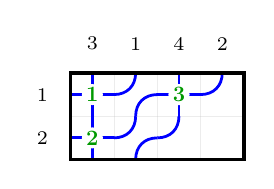
\begin{tikzpicture}[scale=0.55]
  \draw[lightgray, very thin, opacity=0.3] (0,2) -- (4,2);
  \draw[lightgray, very thin, opacity=0.3] (0,3) -- (4,3);
  \draw[lightgray, very thin, opacity=0.3] (0,4) -- (4,4);
  \draw[lightgray, very thin, opacity=0.3] (0,2) -- (0,4);
  \draw[lightgray, very thin, opacity=0.3] (1,2) -- (1,4);
  \draw[lightgray, very thin, opacity=0.3] (2,2) -- (2,4);
  \draw[lightgray, very thin, opacity=0.3] (3,2) -- (3,4);
  \draw[lightgray, very thin, opacity=0.3] (4,2) -- (4,4);
  \draw[blue, line width=1.0pt, line cap=round] (0,3.5) -- (1,3.5);
  \draw[blue, line width=1.0pt, line cap=round] (0.5,3) -- (0.5,4);
  \draw[blue, line width=1.0pt] (1,3.5) .. controls (1.3,3.5) and (1.5,3.7) .. (1.5,4);
  \draw[blue, line width=1.0pt] (1.5,3) .. controls (1.5,3.3) and (1.7,3.5) .. (2,3.5);
  \draw[blue, line width=1.0pt, line cap=round] (2,3.5) -- (3,3.5);
  \draw[blue, line width=1.0pt, line cap=round] (2.5,3) -- (2.5,4);
  \draw[blue, line width=1.0pt] (3,3.5) .. controls (3.3,3.5) and (3.5,3.7) .. (3.5,4);
  \draw[blue, line width=1.0pt, line cap=round] (0,2.5) -- (1,2.5);
  \draw[blue, line width=1.0pt, line cap=round] (0.5,2) -- (0.5,3);
  \draw[blue, line width=1.0pt] (1,2.5) .. controls (1.3,2.5) and (1.5,2.7) .. (1.5,3);
  \draw[blue, line width=1.0pt] (1.5,2) .. controls (1.5,2.3) and (1.7,2.5) .. (2,2.5);
  \draw[blue, line width=1.0pt] (2,2.5) .. controls (2.3,2.5) and (2.5,2.7) .. (2.5,3);
  \node[font=\Large\bfseries, text=green!60!black, fill=white, inner sep=0.5pt, circle, transform shape] at (0.5,3.5) {1};
  \node[font=\Large\bfseries, text=green!60!black, fill=white, inner sep=0.5pt, circle, transform shape] at (2.5,3.5) {3};
  \node[font=\Large\bfseries, text=green!60!black, fill=white, inner sep=0.5pt, circle, transform shape] at (0.5,2.5) {2};
  \node[font=\scriptsize, text=black, anchor=south] at (0.5,4.3) {3};
  \node[font=\scriptsize, text=black, anchor=south] at (1.5,4.3) {1};
  \node[font=\scriptsize, text=black, anchor=south] at (2.5,4.3) {4};
  \node[font=\scriptsize, text=black, anchor=south] at (3.5,4.3) {2};
  \node[font=\scriptsize, text=black, anchor=east] at (-0.3,3.5) {1};
  \node[font=\scriptsize, text=black, anchor=east] at (-0.3,2.5) {2};
  \draw[black, line width=1.2000000000000002pt] (0,2) rectangle (4,4);
\end{tikzpicture}}}
  \sqcupplus
  \vcenter{\hbox{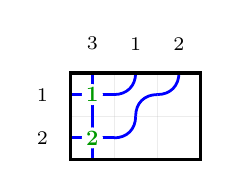
\begin{tikzpicture}[scale=0.55]
  \draw[lightgray, very thin, opacity=0.3] (0,1) -- (3,1);
  \draw[lightgray, very thin, opacity=0.3] (0,2) -- (3,2);
  \draw[lightgray, very thin, opacity=0.3] (0,3) -- (3,3);
  \draw[lightgray, very thin, opacity=0.3] (0,1) -- (0,3);
  \draw[lightgray, very thin, opacity=0.3] (1,1) -- (1,3);
  \draw[lightgray, very thin, opacity=0.3] (2,1) -- (2,3);
  \draw[lightgray, very thin, opacity=0.3] (3,1) -- (3,3);
  \draw[blue, line width=1.0pt, line cap=round] (0,2.5) -- (1,2.5);
  \draw[blue, line width=1.0pt, line cap=round] (0.5,2) -- (0.5,3);
  \draw[blue, line width=1.0pt] (1,2.5) .. controls (1.3,2.5) and (1.5,2.7) .. (1.5,3);
  \draw[blue, line width=1.0pt] (1.5,2) .. controls (1.5,2.3) and (1.7,2.5) .. (2,2.5);
  \draw[blue, line width=1.0pt] (2,2.5) .. controls (2.3,2.5) and (2.5,2.7) .. (2.5,3);
  \draw[blue, line width=1.0pt, line cap=round] (0,1.5) -- (1,1.5);
  \draw[blue, line width=1.0pt, line cap=round] (0.5,1) -- (0.5,2);
  \draw[blue, line width=1.0pt] (1,1.5) .. controls (1.3,1.5) and (1.5,1.7) .. (1.5,2);
  \node[font=\Large\bfseries, text=green!60!black, fill=white, inner sep=0.5pt, circle, transform shape] at (0.5,2.5) {1};
  \node[font=\Large\bfseries, text=green!60!black, fill=white, inner sep=0.5pt, circle, transform shape] at (0.5,1.5) {2};
  \node[font=\scriptsize, text=black, anchor=south] at (0.5,3.3) {3};
  \node[font=\scriptsize, text=black, anchor=south] at (1.5,3.3) {1};
  \node[font=\scriptsize, text=black, anchor=south] at (2.5,3.3) {2};
  \node[font=\scriptsize, text=black, anchor=east] at (-0.3,2.5) {1};
  \node[font=\scriptsize, text=black, anchor=east] at (-0.3,1.5) {2};
  \draw[black, line width=1.2000000000000002pt] (0,1) rectangle (3,3);
\end{tikzpicture}}}
  \\[1em]
  ={}& 
  \vcenter{\hbox{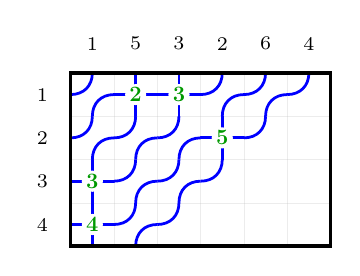
\begin{tikzpicture}[scale=0.55]
  \draw[lightgray, very thin, opacity=0.3] (0,2) -- (6,2);
  \draw[lightgray, very thin, opacity=0.3] (0,3) -- (6,3);
  \draw[lightgray, very thin, opacity=0.3] (0,4) -- (6,4);
  \draw[lightgray, very thin, opacity=0.3] (0,5) -- (6,5);
  \draw[lightgray, very thin, opacity=0.3] (0,6) -- (6,6);
  \draw[lightgray, very thin, opacity=0.3] (0,2) -- (0,6);
  \draw[lightgray, very thin, opacity=0.3] (1,2) -- (1,6);
  \draw[lightgray, very thin, opacity=0.3] (2,2) -- (2,6);
  \draw[lightgray, very thin, opacity=0.3] (3,2) -- (3,6);
  \draw[lightgray, very thin, opacity=0.3] (4,2) -- (4,6);
  \draw[lightgray, very thin, opacity=0.3] (5,2) -- (5,6);
  \draw[lightgray, very thin, opacity=0.3] (6,2) -- (6,6);
  \draw[blue, line width=1.0pt] (0,5.5) .. controls (0.3,5.5) and (0.5,5.7) .. (0.5,6);
  \draw[blue, line width=1.0pt] (0.5,5) .. controls (0.5,5.3) and (0.7,5.5) .. (1,5.5);
  \draw[blue, line width=1.0pt, line cap=round] (1,5.5) -- (2,5.5);
  \draw[blue, line width=1.0pt, line cap=round] (1.5,5) -- (1.5,6);
  \draw[blue, line width=1.0pt, line cap=round] (2,5.5) -- (3,5.5);
  \draw[blue, line width=1.0pt, line cap=round] (2.5,5) -- (2.5,6);
  \draw[blue, line width=1.0pt] (3,5.5) .. controls (3.3,5.5) and (3.5,5.7) .. (3.5,6);
  \draw[blue, line width=1.0pt] (3.5,5) .. controls (3.5,5.3) and (3.7,5.5) .. (4,5.5);
  \draw[blue, line width=1.0pt] (4,5.5) .. controls (4.3,5.5) and (4.5,5.7) .. (4.5,6);
  \draw[blue, line width=1.0pt] (4.5,5) .. controls (4.5,5.3) and (4.7,5.5) .. (5,5.5);
  \draw[blue, line width=1.0pt] (5,5.5) .. controls (5.3,5.5) and (5.5,5.7) .. (5.5,6);
  \draw[blue, line width=1.0pt] (0,4.5) .. controls (0.3,4.5) and (0.5,4.7) .. (0.5,5);
  \draw[blue, line width=1.0pt] (0.5,4) .. controls (0.5,4.3) and (0.7,4.5) .. (1,4.5);
  \draw[blue, line width=1.0pt] (1,4.5) .. controls (1.3,4.5) and (1.5,4.7) .. (1.5,5);
  \draw[blue, line width=1.0pt] (1.5,4) .. controls (1.5,4.3) and (1.7,4.5) .. (2,4.5);
  \draw[blue, line width=1.0pt] (2,4.5) .. controls (2.3,4.5) and (2.5,4.7) .. (2.5,5);
  \draw[blue, line width=1.0pt] (2.5,4) .. controls (2.5,4.3) and (2.7,4.5) .. (3,4.5);
  \draw[blue, line width=1.0pt, line cap=round] (3,4.5) -- (4,4.5);
  \draw[blue, line width=1.0pt, line cap=round] (3.5,4) -- (3.5,5);
  \draw[blue, line width=1.0pt] (4,4.5) .. controls (4.3,4.5) and (4.5,4.7) .. (4.5,5);
  \draw[blue, line width=1.0pt, line cap=round] (0,3.5) -- (1,3.5);
  \draw[blue, line width=1.0pt, line cap=round] (0.5,3) -- (0.5,4);
  \draw[blue, line width=1.0pt] (1,3.5) .. controls (1.3,3.5) and (1.5,3.7) .. (1.5,4);
  \draw[blue, line width=1.0pt] (1.5,3) .. controls (1.5,3.3) and (1.7,3.5) .. (2,3.5);
  \draw[blue, line width=1.0pt] (2,3.5) .. controls (2.3,3.5) and (2.5,3.7) .. (2.5,4);
  \draw[blue, line width=1.0pt] (2.5,3) .. controls (2.5,3.3) and (2.7,3.5) .. (3,3.5);
  \draw[blue, line width=1.0pt] (3,3.5) .. controls (3.3,3.5) and (3.5,3.7) .. (3.5,4);
  \draw[blue, line width=1.0pt, line cap=round] (0,2.5) -- (1,2.5);
  \draw[blue, line width=1.0pt, line cap=round] (0.5,2) -- (0.5,3);
  \draw[blue, line width=1.0pt] (1,2.5) .. controls (1.3,2.5) and (1.5,2.7) .. (1.5,3);
  \draw[blue, line width=1.0pt] (1.5,2) .. controls (1.5,2.3) and (1.7,2.5) .. (2,2.5);
  \draw[blue, line width=1.0pt] (2,2.5) .. controls (2.3,2.5) and (2.5,2.7) .. (2.5,3);
  \node[font=\Large\bfseries, text=green!60!black, fill=white, inner sep=0.5pt, circle, transform shape] at (3.5,4.5) {5};
  \node[font=\Large\bfseries, text=green!60!black, fill=white, inner sep=0.5pt, circle, transform shape] at (1.5,5.5) {2};
  \node[font=\Large\bfseries, text=green!60!black, fill=white, inner sep=0.5pt, circle, transform shape] at (0.5,2.5) {4};
  \node[font=\Large\bfseries, text=green!60!black, fill=white, inner sep=0.5pt, circle, transform shape] at (0.5,3.5) {3};
  \node[font=\Large\bfseries, text=green!60!black, fill=white, inner sep=0.5pt, circle, transform shape] at (2.5,5.5) {3};
  \node[font=\scriptsize, text=black, anchor=south] at (0.5,6.3) {1};
  \node[font=\scriptsize, text=black, anchor=south] at (1.5,6.3) {5};
  \node[font=\scriptsize, text=black, anchor=south] at (2.5,6.3) {3};
  \node[font=\scriptsize, text=black, anchor=south] at (3.5,6.3) {2};
  \node[font=\scriptsize, text=black, anchor=south] at (4.5,6.3) {6};
  \node[font=\scriptsize, text=black, anchor=south] at (5.5,6.3) {4};
  \node[font=\scriptsize, text=black, anchor=east] at (-0.3,5.5) {1};
  \node[font=\scriptsize, text=black, anchor=east] at (-0.3,4.5) {2};
  \node[font=\scriptsize, text=black, anchor=east] at (-0.3,3.5) {3};
  \node[font=\scriptsize, text=black, anchor=east] at (-0.3,2.5) {4};
  \draw[black, line width=1.2000000000000002pt] (0,2) rectangle (6,6);
\end{tikzpicture}}}
  +
  \vcenter{\hbox{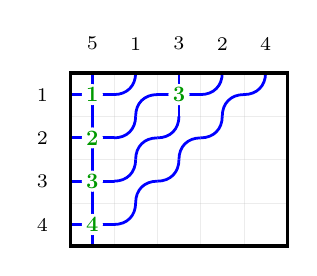
\begin{tikzpicture}[scale=0.55]
  \draw[lightgray, very thin, opacity=0.3] (0,1) -- (5,1);
  \draw[lightgray, very thin, opacity=0.3] (0,2) -- (5,2);
  \draw[lightgray, very thin, opacity=0.3] (0,3) -- (5,3);
  \draw[lightgray, very thin, opacity=0.3] (0,4) -- (5,4);
  \draw[lightgray, very thin, opacity=0.3] (0,5) -- (5,5);
  \draw[lightgray, very thin, opacity=0.3] (0,1) -- (0,5);
  \draw[lightgray, very thin, opacity=0.3] (1,1) -- (1,5);
  \draw[lightgray, very thin, opacity=0.3] (2,1) -- (2,5);
  \draw[lightgray, very thin, opacity=0.3] (3,1) -- (3,5);
  \draw[lightgray, very thin, opacity=0.3] (4,1) -- (4,5);
  \draw[lightgray, very thin, opacity=0.3] (5,1) -- (5,5);
  \draw[blue, line width=1.0pt, line cap=round] (0,4.5) -- (1,4.5);
  \draw[blue, line width=1.0pt, line cap=round] (0.5,4) -- (0.5,5);
  \draw[blue, line width=1.0pt] (1,4.5) .. controls (1.3,4.5) and (1.5,4.7) .. (1.5,5);
  \draw[blue, line width=1.0pt] (1.5,4) .. controls (1.5,4.3) and (1.7,4.5) .. (2,4.5);
  \draw[blue, line width=1.0pt, line cap=round] (2,4.5) -- (3,4.5);
  \draw[blue, line width=1.0pt, line cap=round] (2.5,4) -- (2.5,5);
  \draw[blue, line width=1.0pt] (3,4.5) .. controls (3.3,4.5) and (3.5,4.7) .. (3.5,5);
  \draw[blue, line width=1.0pt] (3.5,4) .. controls (3.5,4.3) and (3.7,4.5) .. (4,4.5);
  \draw[blue, line width=1.0pt] (4,4.5) .. controls (4.3,4.5) and (4.5,4.7) .. (4.5,5);
  \draw[blue, line width=1.0pt, line cap=round] (0,3.5) -- (1,3.5);
  \draw[blue, line width=1.0pt, line cap=round] (0.5,3) -- (0.5,4);
  \draw[blue, line width=1.0pt] (1,3.5) .. controls (1.3,3.5) and (1.5,3.7) .. (1.5,4);
  \draw[blue, line width=1.0pt] (1.5,3) .. controls (1.5,3.3) and (1.7,3.5) .. (2,3.5);
  \draw[blue, line width=1.0pt] (2,3.5) .. controls (2.3,3.5) and (2.5,3.7) .. (2.5,4);
  \draw[blue, line width=1.0pt] (2.5,3) .. controls (2.5,3.3) and (2.7,3.5) .. (3,3.5);
  \draw[blue, line width=1.0pt] (3,3.5) .. controls (3.3,3.5) and (3.5,3.7) .. (3.5,4);
  \draw[blue, line width=1.0pt, line cap=round] (0,2.5) -- (1,2.5);
  \draw[blue, line width=1.0pt, line cap=round] (0.5,2) -- (0.5,3);
  \draw[blue, line width=1.0pt] (1,2.5) .. controls (1.3,2.5) and (1.5,2.7) .. (1.5,3);
  \draw[blue, line width=1.0pt] (1.5,2) .. controls (1.5,2.3) and (1.7,2.5) .. (2,2.5);
  \draw[blue, line width=1.0pt] (2,2.5) .. controls (2.3,2.5) and (2.5,2.7) .. (2.5,3);
  \draw[blue, line width=1.0pt, line cap=round] (0,1.5) -- (1,1.5);
  \draw[blue, line width=1.0pt, line cap=round] (0.5,1) -- (0.5,2);
  \draw[blue, line width=1.0pt] (1,1.5) .. controls (1.3,1.5) and (1.5,1.7) .. (1.5,2);
  \node[font=\Large\bfseries, text=green!60!black, fill=white, inner sep=0.5pt, circle, transform shape] at (0.5,3.5) {2};
  \node[font=\Large\bfseries, text=green!60!black, fill=white, inner sep=0.5pt, circle, transform shape] at (0.5,1.5) {4};
  \node[font=\Large\bfseries, text=green!60!black, fill=white, inner sep=0.5pt, circle, transform shape] at (0.5,2.5) {3};
  \node[font=\Large\bfseries, text=green!60!black, fill=white, inner sep=0.5pt, circle, transform shape] at (0.5,4.5) {1};
  \node[font=\Large\bfseries, text=green!60!black, fill=white, inner sep=0.5pt, circle, transform shape] at (2.5,4.5) {3};
  \node[font=\scriptsize, text=black, anchor=south] at (0.5,5.3) {5};
  \node[font=\scriptsize, text=black, anchor=south] at (1.5,5.3) {1};
  \node[font=\scriptsize, text=black, anchor=south] at (2.5,5.3) {3};
  \node[font=\scriptsize, text=black, anchor=south] at (3.5,5.3) {2};
  \node[font=\scriptsize, text=black, anchor=south] at (4.5,5.3) {4};
  \node[font=\scriptsize, text=black, anchor=east] at (-0.3,4.5) {1};
  \node[font=\scriptsize, text=black, anchor=east] at (-0.3,3.5) {2};
  \node[font=\scriptsize, text=black, anchor=east] at (-0.3,2.5) {3};
  \node[font=\scriptsize, text=black, anchor=east] at (-0.3,1.5) {4};
  \draw[black, line width=1.2000000000000002pt] (0,1) rectangle (5,5);
\end{tikzpicture}}}
  +
  \vcenter{\hbox{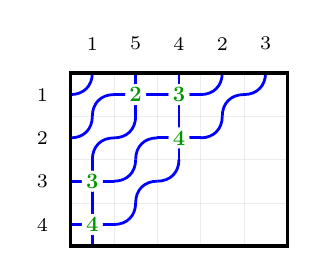
\begin{tikzpicture}[scale=0.55]
  \draw[lightgray, very thin, opacity=0.3] (0,1) -- (5,1);
  \draw[lightgray, very thin, opacity=0.3] (0,2) -- (5,2);
  \draw[lightgray, very thin, opacity=0.3] (0,3) -- (5,3);
  \draw[lightgray, very thin, opacity=0.3] (0,4) -- (5,4);
  \draw[lightgray, very thin, opacity=0.3] (0,5) -- (5,5);
  \draw[lightgray, very thin, opacity=0.3] (0,1) -- (0,5);
  \draw[lightgray, very thin, opacity=0.3] (1,1) -- (1,5);
  \draw[lightgray, very thin, opacity=0.3] (2,1) -- (2,5);
  \draw[lightgray, very thin, opacity=0.3] (3,1) -- (3,5);
  \draw[lightgray, very thin, opacity=0.3] (4,1) -- (4,5);
  \draw[lightgray, very thin, opacity=0.3] (5,1) -- (5,5);
  \draw[blue, line width=1.0pt] (0,4.5) .. controls (0.3,4.5) and (0.5,4.7) .. (0.5,5);
  \draw[blue, line width=1.0pt] (0.5,4) .. controls (0.5,4.3) and (0.7,4.5) .. (1,4.5);
  \draw[blue, line width=1.0pt, line cap=round] (1,4.5) -- (2,4.5);
  \draw[blue, line width=1.0pt, line cap=round] (1.5,4) -- (1.5,5);
  \draw[blue, line width=1.0pt, line cap=round] (2,4.5) -- (3,4.5);
  \draw[blue, line width=1.0pt, line cap=round] (2.5,4) -- (2.5,5);
  \draw[blue, line width=1.0pt] (3,4.5) .. controls (3.3,4.5) and (3.5,4.7) .. (3.5,5);
  \draw[blue, line width=1.0pt] (3.5,4) .. controls (3.5,4.3) and (3.7,4.5) .. (4,4.5);
  \draw[blue, line width=1.0pt] (4,4.5) .. controls (4.3,4.5) and (4.5,4.7) .. (4.5,5);
  \draw[blue, line width=1.0pt] (0,3.5) .. controls (0.3,3.5) and (0.5,3.7) .. (0.5,4);
  \draw[blue, line width=1.0pt] (0.5,3) .. controls (0.5,3.3) and (0.7,3.5) .. (1,3.5);
  \draw[blue, line width=1.0pt] (1,3.5) .. controls (1.3,3.5) and (1.5,3.7) .. (1.5,4);
  \draw[blue, line width=1.0pt] (1.5,3) .. controls (1.5,3.3) and (1.7,3.5) .. (2,3.5);
  \draw[blue, line width=1.0pt, line cap=round] (2,3.5) -- (3,3.5);
  \draw[blue, line width=1.0pt, line cap=round] (2.5,3) -- (2.5,4);
  \draw[blue, line width=1.0pt] (3,3.5) .. controls (3.3,3.5) and (3.5,3.7) .. (3.5,4);
  \draw[blue, line width=1.0pt, line cap=round] (0,2.5) -- (1,2.5);
  \draw[blue, line width=1.0pt, line cap=round] (0.5,2) -- (0.5,3);
  \draw[blue, line width=1.0pt] (1,2.5) .. controls (1.3,2.5) and (1.5,2.7) .. (1.5,3);
  \draw[blue, line width=1.0pt] (1.5,2) .. controls (1.5,2.3) and (1.7,2.5) .. (2,2.5);
  \draw[blue, line width=1.0pt] (2,2.5) .. controls (2.3,2.5) and (2.5,2.7) .. (2.5,3);
  \draw[blue, line width=1.0pt, line cap=round] (0,1.5) -- (1,1.5);
  \draw[blue, line width=1.0pt, line cap=round] (0.5,1) -- (0.5,2);
  \draw[blue, line width=1.0pt] (1,1.5) .. controls (1.3,1.5) and (1.5,1.7) .. (1.5,2);
  \node[font=\Large\bfseries, text=green!60!black, fill=white, inner sep=0.5pt, circle, transform shape] at (1.5,4.5) {2};
  \node[font=\Large\bfseries, text=green!60!black, fill=white, inner sep=0.5pt, circle, transform shape] at (0.5,1.5) {4};
  \node[font=\Large\bfseries, text=green!60!black, fill=white, inner sep=0.5pt, circle, transform shape] at (0.5,2.5) {3};
  \node[font=\Large\bfseries, text=green!60!black, fill=white, inner sep=0.5pt, circle, transform shape] at (2.5,3.5) {4};
  \node[font=\Large\bfseries, text=green!60!black, fill=white, inner sep=0.5pt, circle, transform shape] at (2.5,4.5) {3};
  \node[font=\scriptsize, text=black, anchor=south] at (0.5,5.3) {1};
  \node[font=\scriptsize, text=black, anchor=south] at (1.5,5.3) {5};
  \node[font=\scriptsize, text=black, anchor=south] at (2.5,5.3) {4};
  \node[font=\scriptsize, text=black, anchor=south] at (3.5,5.3) {2};
  \node[font=\scriptsize, text=black, anchor=south] at (4.5,5.3) {3};
  \node[font=\scriptsize, text=black, anchor=east] at (-0.3,4.5) {1};
  \node[font=\scriptsize, text=black, anchor=east] at (-0.3,3.5) {2};
  \node[font=\scriptsize, text=black, anchor=east] at (-0.3,2.5) {3};
  \node[font=\scriptsize, text=black, anchor=east] at (-0.3,1.5) {4};
  \draw[black, line width=1.2000000000000002pt] (0,1) rectangle (5,5);
\end{tikzpicture}}}
  \\[1em]
  + & 
  \vcenter{\hbox{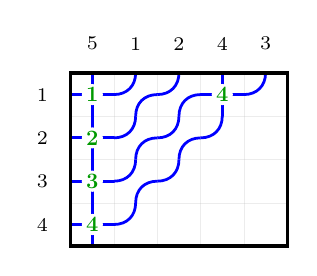
\begin{tikzpicture}[scale=0.55]
  \draw[lightgray, very thin, opacity=0.3] (0,1) -- (5,1);
  \draw[lightgray, very thin, opacity=0.3] (0,2) -- (5,2);
  \draw[lightgray, very thin, opacity=0.3] (0,3) -- (5,3);
  \draw[lightgray, very thin, opacity=0.3] (0,4) -- (5,4);
  \draw[lightgray, very thin, opacity=0.3] (0,5) -- (5,5);
  \draw[lightgray, very thin, opacity=0.3] (0,1) -- (0,5);
  \draw[lightgray, very thin, opacity=0.3] (1,1) -- (1,5);
  \draw[lightgray, very thin, opacity=0.3] (2,1) -- (2,5);
  \draw[lightgray, very thin, opacity=0.3] (3,1) -- (3,5);
  \draw[lightgray, very thin, opacity=0.3] (4,1) -- (4,5);
  \draw[lightgray, very thin, opacity=0.3] (5,1) -- (5,5);
  \draw[blue, line width=1.0pt, line cap=round] (0,4.5) -- (1,4.5);
  \draw[blue, line width=1.0pt, line cap=round] (0.5,4) -- (0.5,5);
  \draw[blue, line width=1.0pt] (1,4.5) .. controls (1.3,4.5) and (1.5,4.7) .. (1.5,5);
  \draw[blue, line width=1.0pt] (1.5,4) .. controls (1.5,4.3) and (1.7,4.5) .. (2,4.5);
  \draw[blue, line width=1.0pt] (2,4.5) .. controls (2.3,4.5) and (2.5,4.7) .. (2.5,5);
  \draw[blue, line width=1.0pt] (2.5,4) .. controls (2.5,4.3) and (2.7,4.5) .. (3,4.5);
  \draw[blue, line width=1.0pt, line cap=round] (3,4.5) -- (4,4.5);
  \draw[blue, line width=1.0pt, line cap=round] (3.5,4) -- (3.5,5);
  \draw[blue, line width=1.0pt] (4,4.5) .. controls (4.3,4.5) and (4.5,4.7) .. (4.5,5);
  \draw[blue, line width=1.0pt, line cap=round] (0,3.5) -- (1,3.5);
  \draw[blue, line width=1.0pt, line cap=round] (0.5,3) -- (0.5,4);
  \draw[blue, line width=1.0pt] (1,3.5) .. controls (1.3,3.5) and (1.5,3.7) .. (1.5,4);
  \draw[blue, line width=1.0pt] (1.5,3) .. controls (1.5,3.3) and (1.7,3.5) .. (2,3.5);
  \draw[blue, line width=1.0pt] (2,3.5) .. controls (2.3,3.5) and (2.5,3.7) .. (2.5,4);
  \draw[blue, line width=1.0pt] (2.5,3) .. controls (2.5,3.3) and (2.7,3.5) .. (3,3.5);
  \draw[blue, line width=1.0pt] (3,3.5) .. controls (3.3,3.5) and (3.5,3.7) .. (3.5,4);
  \draw[blue, line width=1.0pt, line cap=round] (0,2.5) -- (1,2.5);
  \draw[blue, line width=1.0pt, line cap=round] (0.5,2) -- (0.5,3);
  \draw[blue, line width=1.0pt] (1,2.5) .. controls (1.3,2.5) and (1.5,2.7) .. (1.5,3);
  \draw[blue, line width=1.0pt] (1.5,2) .. controls (1.5,2.3) and (1.7,2.5) .. (2,2.5);
  \draw[blue, line width=1.0pt] (2,2.5) .. controls (2.3,2.5) and (2.5,2.7) .. (2.5,3);
  \draw[blue, line width=1.0pt, line cap=round] (0,1.5) -- (1,1.5);
  \draw[blue, line width=1.0pt, line cap=round] (0.5,1) -- (0.5,2);
  \draw[blue, line width=1.0pt] (1,1.5) .. controls (1.3,1.5) and (1.5,1.7) .. (1.5,2);
  \node[font=\Large\bfseries, text=green!60!black, fill=white, inner sep=0.5pt, circle, transform shape] at (0.5,3.5) {2};
  \node[font=\Large\bfseries, text=green!60!black, fill=white, inner sep=0.5pt, circle, transform shape] at (0.5,2.5) {3};
  \node[font=\Large\bfseries, text=green!60!black, fill=white, inner sep=0.5pt, circle, transform shape] at (0.5,4.5) {1};
  \node[font=\Large\bfseries, text=green!60!black, fill=white, inner sep=0.5pt, circle, transform shape] at (3.5,4.5) {4};
  \node[font=\Large\bfseries, text=green!60!black, fill=white, inner sep=0.5pt, circle, transform shape] at (0.5,1.5) {4};
  \node[font=\scriptsize, text=black, anchor=south] at (0.5,5.3) {5};
  \node[font=\scriptsize, text=black, anchor=south] at (1.5,5.3) {1};
  \node[font=\scriptsize, text=black, anchor=south] at (2.5,5.3) {2};
  \node[font=\scriptsize, text=black, anchor=south] at (3.5,5.3) {4};
  \node[font=\scriptsize, text=black, anchor=south] at (4.5,5.3) {3};
  \node[font=\scriptsize, text=black, anchor=east] at (-0.3,4.5) {1};
  \node[font=\scriptsize, text=black, anchor=east] at (-0.3,3.5) {2};
  \node[font=\scriptsize, text=black, anchor=east] at (-0.3,2.5) {3};
  \node[font=\scriptsize, text=black, anchor=east] at (-0.3,1.5) {4};
  \draw[black, line width=1.2000000000000002pt] (0,1) rectangle (5,5);
\end{tikzpicture}}}
  +
  \vcenter{\hbox{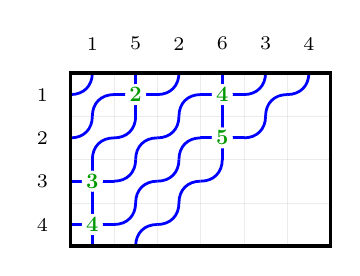
\begin{tikzpicture}[scale=0.55]
  \draw[lightgray, very thin, opacity=0.3] (0,2) -- (6,2);
  \draw[lightgray, very thin, opacity=0.3] (0,3) -- (6,3);
  \draw[lightgray, very thin, opacity=0.3] (0,4) -- (6,4);
  \draw[lightgray, very thin, opacity=0.3] (0,5) -- (6,5);
  \draw[lightgray, very thin, opacity=0.3] (0,6) -- (6,6);
  \draw[lightgray, very thin, opacity=0.3] (0,2) -- (0,6);
  \draw[lightgray, very thin, opacity=0.3] (1,2) -- (1,6);
  \draw[lightgray, very thin, opacity=0.3] (2,2) -- (2,6);
  \draw[lightgray, very thin, opacity=0.3] (3,2) -- (3,6);
  \draw[lightgray, very thin, opacity=0.3] (4,2) -- (4,6);
  \draw[lightgray, very thin, opacity=0.3] (5,2) -- (5,6);
  \draw[lightgray, very thin, opacity=0.3] (6,2) -- (6,6);
  \draw[blue, line width=1.0pt] (0,5.5) .. controls (0.3,5.5) and (0.5,5.7) .. (0.5,6);
  \draw[blue, line width=1.0pt] (0.5,5) .. controls (0.5,5.3) and (0.7,5.5) .. (1,5.5);
  \draw[blue, line width=1.0pt, line cap=round] (1,5.5) -- (2,5.5);
  \draw[blue, line width=1.0pt, line cap=round] (1.5,5) -- (1.5,6);
  \draw[blue, line width=1.0pt] (2,5.5) .. controls (2.3,5.5) and (2.5,5.7) .. (2.5,6);
  \draw[blue, line width=1.0pt] (2.5,5) .. controls (2.5,5.3) and (2.7,5.5) .. (3,5.5);
  \draw[blue, line width=1.0pt, line cap=round] (3,5.5) -- (4,5.5);
  \draw[blue, line width=1.0pt, line cap=round] (3.5,5) -- (3.5,6);
  \draw[blue, line width=1.0pt] (4,5.5) .. controls (4.3,5.5) and (4.5,5.7) .. (4.5,6);
  \draw[blue, line width=1.0pt] (4.5,5) .. controls (4.5,5.3) and (4.7,5.5) .. (5,5.5);
  \draw[blue, line width=1.0pt] (5,5.5) .. controls (5.3,5.5) and (5.5,5.7) .. (5.5,6);
  \draw[blue, line width=1.0pt] (0,4.5) .. controls (0.3,4.5) and (0.5,4.7) .. (0.5,5);
  \draw[blue, line width=1.0pt] (0.5,4) .. controls (0.5,4.3) and (0.7,4.5) .. (1,4.5);
  \draw[blue, line width=1.0pt] (1,4.5) .. controls (1.3,4.5) and (1.5,4.7) .. (1.5,5);
  \draw[blue, line width=1.0pt] (1.5,4) .. controls (1.5,4.3) and (1.7,4.5) .. (2,4.5);
  \draw[blue, line width=1.0pt] (2,4.5) .. controls (2.3,4.5) and (2.5,4.7) .. (2.5,5);
  \draw[blue, line width=1.0pt] (2.5,4) .. controls (2.5,4.3) and (2.7,4.5) .. (3,4.5);
  \draw[blue, line width=1.0pt, line cap=round] (3,4.5) -- (4,4.5);
  \draw[blue, line width=1.0pt, line cap=round] (3.5,4) -- (3.5,5);
  \draw[blue, line width=1.0pt] (4,4.5) .. controls (4.3,4.5) and (4.5,4.7) .. (4.5,5);
  \draw[blue, line width=1.0pt, line cap=round] (0,3.5) -- (1,3.5);
  \draw[blue, line width=1.0pt, line cap=round] (0.5,3) -- (0.5,4);
  \draw[blue, line width=1.0pt] (1,3.5) .. controls (1.3,3.5) and (1.5,3.7) .. (1.5,4);
  \draw[blue, line width=1.0pt] (1.5,3) .. controls (1.5,3.3) and (1.7,3.5) .. (2,3.5);
  \draw[blue, line width=1.0pt] (2,3.5) .. controls (2.3,3.5) and (2.5,3.7) .. (2.5,4);
  \draw[blue, line width=1.0pt] (2.5,3) .. controls (2.5,3.3) and (2.7,3.5) .. (3,3.5);
  \draw[blue, line width=1.0pt] (3,3.5) .. controls (3.3,3.5) and (3.5,3.7) .. (3.5,4);
  \draw[blue, line width=1.0pt, line cap=round] (0,2.5) -- (1,2.5);
  \draw[blue, line width=1.0pt, line cap=round] (0.5,2) -- (0.5,3);
  \draw[blue, line width=1.0pt] (1,2.5) .. controls (1.3,2.5) and (1.5,2.7) .. (1.5,3);
  \draw[blue, line width=1.0pt] (1.5,2) .. controls (1.5,2.3) and (1.7,2.5) .. (2,2.5);
  \draw[blue, line width=1.0pt] (2,2.5) .. controls (2.3,2.5) and (2.5,2.7) .. (2.5,3);
  \node[font=\Large\bfseries, text=green!60!black, fill=white, inner sep=0.5pt, circle, transform shape] at (3.5,4.5) {5};
  \node[font=\Large\bfseries, text=green!60!black, fill=white, inner sep=0.5pt, circle, transform shape] at (1.5,5.5) {2};
  \node[font=\Large\bfseries, text=green!60!black, fill=white, inner sep=0.5pt, circle, transform shape] at (0.5,3.5) {3};
  \node[font=\Large\bfseries, text=green!60!black, fill=white, inner sep=0.5pt, circle, transform shape] at (3.5,5.5) {4};
  \node[font=\Large\bfseries, text=green!60!black, fill=white, inner sep=0.5pt, circle, transform shape] at (0.5,2.5) {4};
  \node[font=\scriptsize, text=black, anchor=south] at (0.5,6.3) {1};
  \node[font=\scriptsize, text=black, anchor=south] at (1.5,6.3) {5};
  \node[font=\scriptsize, text=black, anchor=south] at (2.5,6.3) {2};
  \node[font=\scriptsize, text=black, anchor=south] at (3.5,6.3) {6};
  \node[font=\scriptsize, text=black, anchor=south] at (4.5,6.3) {3};
  \node[font=\scriptsize, text=black, anchor=south] at (5.5,6.3) {4};
  \node[font=\scriptsize, text=black, anchor=east] at (-0.3,5.5) {1};
  \node[font=\scriptsize, text=black, anchor=east] at (-0.3,4.5) {2};
  \node[font=\scriptsize, text=black, anchor=east] at (-0.3,3.5) {3};
  \node[font=\scriptsize, text=black, anchor=east] at (-0.3,2.5) {4};
  \draw[black, line width=1.2000000000000002pt] (0,2) rectangle (6,6);
\end{tikzpicture}}}
  +
  \vcenter{\hbox{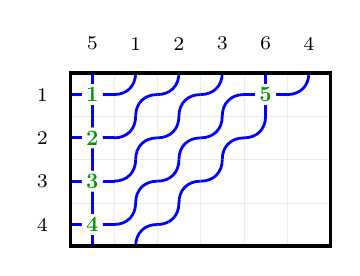
\begin{tikzpicture}[scale=0.55]
  \draw[lightgray, very thin, opacity=0.3] (0,2) -- (6,2);
  \draw[lightgray, very thin, opacity=0.3] (0,3) -- (6,3);
  \draw[lightgray, very thin, opacity=0.3] (0,4) -- (6,4);
  \draw[lightgray, very thin, opacity=0.3] (0,5) -- (6,5);
  \draw[lightgray, very thin, opacity=0.3] (0,6) -- (6,6);
  \draw[lightgray, very thin, opacity=0.3] (0,2) -- (0,6);
  \draw[lightgray, very thin, opacity=0.3] (1,2) -- (1,6);
  \draw[lightgray, very thin, opacity=0.3] (2,2) -- (2,6);
  \draw[lightgray, very thin, opacity=0.3] (3,2) -- (3,6);
  \draw[lightgray, very thin, opacity=0.3] (4,2) -- (4,6);
  \draw[lightgray, very thin, opacity=0.3] (5,2) -- (5,6);
  \draw[lightgray, very thin, opacity=0.3] (6,2) -- (6,6);
  \draw[blue, line width=1.0pt, line cap=round] (0,5.5) -- (1,5.5);
  \draw[blue, line width=1.0pt, line cap=round] (0.5,5) -- (0.5,6);
  \draw[blue, line width=1.0pt] (1,5.5) .. controls (1.3,5.5) and (1.5,5.7) .. (1.5,6);
  \draw[blue, line width=1.0pt] (1.5,5) .. controls (1.5,5.3) and (1.7,5.5) .. (2,5.5);
  \draw[blue, line width=1.0pt] (2,5.5) .. controls (2.3,5.5) and (2.5,5.7) .. (2.5,6);
  \draw[blue, line width=1.0pt] (2.5,5) .. controls (2.5,5.3) and (2.7,5.5) .. (3,5.5);
  \draw[blue, line width=1.0pt] (3,5.5) .. controls (3.3,5.5) and (3.5,5.7) .. (3.5,6);
  \draw[blue, line width=1.0pt] (3.5,5) .. controls (3.5,5.3) and (3.7,5.5) .. (4,5.5);
  \draw[blue, line width=1.0pt, line cap=round] (4,5.5) -- (5,5.5);
  \draw[blue, line width=1.0pt, line cap=round] (4.5,5) -- (4.5,6);
  \draw[blue, line width=1.0pt] (5,5.5) .. controls (5.3,5.5) and (5.5,5.7) .. (5.5,6);
  \draw[blue, line width=1.0pt, line cap=round] (0,4.5) -- (1,4.5);
  \draw[blue, line width=1.0pt, line cap=round] (0.5,4) -- (0.5,5);
  \draw[blue, line width=1.0pt] (1,4.5) .. controls (1.3,4.5) and (1.5,4.7) .. (1.5,5);
  \draw[blue, line width=1.0pt] (1.5,4) .. controls (1.5,4.3) and (1.7,4.5) .. (2,4.5);
  \draw[blue, line width=1.0pt] (2,4.5) .. controls (2.3,4.5) and (2.5,4.7) .. (2.5,5);
  \draw[blue, line width=1.0pt] (2.5,4) .. controls (2.5,4.3) and (2.7,4.5) .. (3,4.5);
  \draw[blue, line width=1.0pt] (3,4.5) .. controls (3.3,4.5) and (3.5,4.7) .. (3.5,5);
  \draw[blue, line width=1.0pt] (3.5,4) .. controls (3.5,4.3) and (3.7,4.5) .. (4,4.5);
  \draw[blue, line width=1.0pt] (4,4.5) .. controls (4.3,4.5) and (4.5,4.7) .. (4.5,5);
  \draw[blue, line width=1.0pt, line cap=round] (0,3.5) -- (1,3.5);
  \draw[blue, line width=1.0pt, line cap=round] (0.5,3) -- (0.5,4);
  \draw[blue, line width=1.0pt] (1,3.5) .. controls (1.3,3.5) and (1.5,3.7) .. (1.5,4);
  \draw[blue, line width=1.0pt] (1.5,3) .. controls (1.5,3.3) and (1.7,3.5) .. (2,3.5);
  \draw[blue, line width=1.0pt] (2,3.5) .. controls (2.3,3.5) and (2.5,3.7) .. (2.5,4);
  \draw[blue, line width=1.0pt] (2.5,3) .. controls (2.5,3.3) and (2.7,3.5) .. (3,3.5);
  \draw[blue, line width=1.0pt] (3,3.5) .. controls (3.3,3.5) and (3.5,3.7) .. (3.5,4);
  \draw[blue, line width=1.0pt, line cap=round] (0,2.5) -- (1,2.5);
  \draw[blue, line width=1.0pt, line cap=round] (0.5,2) -- (0.5,3);
  \draw[blue, line width=1.0pt] (1,2.5) .. controls (1.3,2.5) and (1.5,2.7) .. (1.5,3);
  \draw[blue, line width=1.0pt] (1.5,2) .. controls (1.5,2.3) and (1.7,2.5) .. (2,2.5);
  \draw[blue, line width=1.0pt] (2,2.5) .. controls (2.3,2.5) and (2.5,2.7) .. (2.5,3);
  \node[font=\Large\bfseries, text=green!60!black, fill=white, inner sep=0.5pt, circle, transform shape] at (0.5,4.5) {2};
  \node[font=\Large\bfseries, text=green!60!black, fill=white, inner sep=0.5pt, circle, transform shape] at (4.5,5.5) {5};
  \node[font=\Large\bfseries, text=green!60!black, fill=white, inner sep=0.5pt, circle, transform shape] at (0.5,3.5) {3};
  \node[font=\Large\bfseries, text=green!60!black, fill=white, inner sep=0.5pt, circle, transform shape] at (0.5,5.5) {1};
  \node[font=\Large\bfseries, text=green!60!black, fill=white, inner sep=0.5pt, circle, transform shape] at (0.5,2.5) {4};
  \node[font=\scriptsize, text=black, anchor=south] at (0.5,6.3) {5};
  \node[font=\scriptsize, text=black, anchor=south] at (1.5,6.3) {1};
  \node[font=\scriptsize, text=black, anchor=south] at (2.5,6.3) {2};
  \node[font=\scriptsize, text=black, anchor=south] at (3.5,6.3) {3};
  \node[font=\scriptsize, text=black, anchor=south] at (4.5,6.3) {6};
  \node[font=\scriptsize, text=black, anchor=south] at (5.5,6.3) {4};
  \node[font=\scriptsize, text=black, anchor=east] at (-0.3,5.5) {1};
  \node[font=\scriptsize, text=black, anchor=east] at (-0.3,4.5) {2};
  \node[font=\scriptsize, text=black, anchor=east] at (-0.3,3.5) {3};
  \node[font=\scriptsize, text=black, anchor=east] at (-0.3,2.5) {4};
  \draw[black, line width=1.2000000000000002pt] (0,2) rectangle (6,6);
\end{tikzpicture}}}
  \\[1em]
  + & 
  \vcenter{\hbox{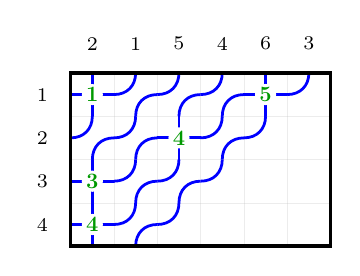
\begin{tikzpicture}[scale=0.55]
  \draw[lightgray, very thin, opacity=0.3] (0,2) -- (6,2);
  \draw[lightgray, very thin, opacity=0.3] (0,3) -- (6,3);
  \draw[lightgray, very thin, opacity=0.3] (0,4) -- (6,4);
  \draw[lightgray, very thin, opacity=0.3] (0,5) -- (6,5);
  \draw[lightgray, very thin, opacity=0.3] (0,6) -- (6,6);
  \draw[lightgray, very thin, opacity=0.3] (0,2) -- (0,6);
  \draw[lightgray, very thin, opacity=0.3] (1,2) -- (1,6);
  \draw[lightgray, very thin, opacity=0.3] (2,2) -- (2,6);
  \draw[lightgray, very thin, opacity=0.3] (3,2) -- (3,6);
  \draw[lightgray, very thin, opacity=0.3] (4,2) -- (4,6);
  \draw[lightgray, very thin, opacity=0.3] (5,2) -- (5,6);
  \draw[lightgray, very thin, opacity=0.3] (6,2) -- (6,6);
  \draw[blue, line width=1.0pt, line cap=round] (0,5.5) -- (1,5.5);
  \draw[blue, line width=1.0pt, line cap=round] (0.5,5) -- (0.5,6);
  \draw[blue, line width=1.0pt] (1,5.5) .. controls (1.3,5.5) and (1.5,5.7) .. (1.5,6);
  \draw[blue, line width=1.0pt] (1.5,5) .. controls (1.5,5.3) and (1.7,5.5) .. (2,5.5);
  \draw[blue, line width=1.0pt] (2,5.5) .. controls (2.3,5.5) and (2.5,5.7) .. (2.5,6);
  \draw[blue, line width=1.0pt] (2.5,5) .. controls (2.5,5.3) and (2.7,5.5) .. (3,5.5);
  \draw[blue, line width=1.0pt] (3,5.5) .. controls (3.3,5.5) and (3.5,5.7) .. (3.5,6);
  \draw[blue, line width=1.0pt] (3.5,5) .. controls (3.5,5.3) and (3.7,5.5) .. (4,5.5);
  \draw[blue, line width=1.0pt, line cap=round] (4,5.5) -- (5,5.5);
  \draw[blue, line width=1.0pt, line cap=round] (4.5,5) -- (4.5,6);
  \draw[blue, line width=1.0pt] (5,5.5) .. controls (5.3,5.5) and (5.5,5.7) .. (5.5,6);
  \draw[blue, line width=1.0pt] (0,4.5) .. controls (0.3,4.5) and (0.5,4.7) .. (0.5,5);
  \draw[blue, line width=1.0pt] (0.5,4) .. controls (0.5,4.3) and (0.7,4.5) .. (1,4.5);
  \draw[blue, line width=1.0pt] (1,4.5) .. controls (1.3,4.5) and (1.5,4.7) .. (1.5,5);
  \draw[blue, line width=1.0pt] (1.5,4) .. controls (1.5,4.3) and (1.7,4.5) .. (2,4.5);
  \draw[blue, line width=1.0pt, line cap=round] (2,4.5) -- (3,4.5);
  \draw[blue, line width=1.0pt, line cap=round] (2.5,4) -- (2.5,5);
  \draw[blue, line width=1.0pt] (3,4.5) .. controls (3.3,4.5) and (3.5,4.7) .. (3.5,5);
  \draw[blue, line width=1.0pt] (3.5,4) .. controls (3.5,4.3) and (3.7,4.5) .. (4,4.5);
  \draw[blue, line width=1.0pt] (4,4.5) .. controls (4.3,4.5) and (4.5,4.7) .. (4.5,5);
  \draw[blue, line width=1.0pt, line cap=round] (0,3.5) -- (1,3.5);
  \draw[blue, line width=1.0pt, line cap=round] (0.5,3) -- (0.5,4);
  \draw[blue, line width=1.0pt] (1,3.5) .. controls (1.3,3.5) and (1.5,3.7) .. (1.5,4);
  \draw[blue, line width=1.0pt] (1.5,3) .. controls (1.5,3.3) and (1.7,3.5) .. (2,3.5);
  \draw[blue, line width=1.0pt] (2,3.5) .. controls (2.3,3.5) and (2.5,3.7) .. (2.5,4);
  \draw[blue, line width=1.0pt] (2.5,3) .. controls (2.5,3.3) and (2.7,3.5) .. (3,3.5);
  \draw[blue, line width=1.0pt] (3,3.5) .. controls (3.3,3.5) and (3.5,3.7) .. (3.5,4);
  \draw[blue, line width=1.0pt, line cap=round] (0,2.5) -- (1,2.5);
  \draw[blue, line width=1.0pt, line cap=round] (0.5,2) -- (0.5,3);
  \draw[blue, line width=1.0pt] (1,2.5) .. controls (1.3,2.5) and (1.5,2.7) .. (1.5,3);
  \draw[blue, line width=1.0pt] (1.5,2) .. controls (1.5,2.3) and (1.7,2.5) .. (2,2.5);
  \draw[blue, line width=1.0pt] (2,2.5) .. controls (2.3,2.5) and (2.5,2.7) .. (2.5,3);
  \node[font=\Large\bfseries, text=green!60!black, fill=white, inner sep=0.5pt, circle, transform shape] at (4.5,5.5) {5};
  \node[font=\Large\bfseries, text=green!60!black, fill=white, inner sep=0.5pt, circle, transform shape] at (0.5,3.5) {3};
  \node[font=\Large\bfseries, text=green!60!black, fill=white, inner sep=0.5pt, circle, transform shape] at (0.5,5.5) {1};
  \node[font=\Large\bfseries, text=green!60!black, fill=white, inner sep=0.5pt, circle, transform shape] at (2.5,4.5) {4};
  \node[font=\Large\bfseries, text=green!60!black, fill=white, inner sep=0.5pt, circle, transform shape] at (0.5,2.5) {4};
  \node[font=\scriptsize, text=black, anchor=south] at (0.5,6.3) {2};
  \node[font=\scriptsize, text=black, anchor=south] at (1.5,6.3) {1};
  \node[font=\scriptsize, text=black, anchor=south] at (2.5,6.3) {5};
  \node[font=\scriptsize, text=black, anchor=south] at (3.5,6.3) {4};
  \node[font=\scriptsize, text=black, anchor=south] at (4.5,6.3) {6};
  \node[font=\scriptsize, text=black, anchor=south] at (5.5,6.3) {3};
  \node[font=\scriptsize, text=black, anchor=east] at (-0.3,5.5) {1};
  \node[font=\scriptsize, text=black, anchor=east] at (-0.3,4.5) {2};
  \node[font=\scriptsize, text=black, anchor=east] at (-0.3,3.5) {3};
  \node[font=\scriptsize, text=black, anchor=east] at (-0.3,2.5) {4};
  \draw[black, line width=1.2000000000000002pt] (0,2) rectangle (6,6);
\end{tikzpicture}}}
  +
  \vcenter{\hbox{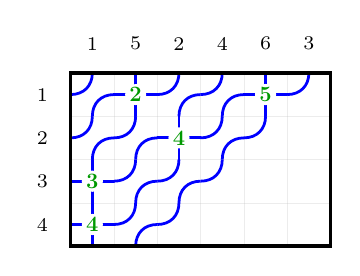
\begin{tikzpicture}[scale=0.55]
  \draw[lightgray, very thin, opacity=0.3] (0,2) -- (6,2);
  \draw[lightgray, very thin, opacity=0.3] (0,3) -- (6,3);
  \draw[lightgray, very thin, opacity=0.3] (0,4) -- (6,4);
  \draw[lightgray, very thin, opacity=0.3] (0,5) -- (6,5);
  \draw[lightgray, very thin, opacity=0.3] (0,6) -- (6,6);
  \draw[lightgray, very thin, opacity=0.3] (0,2) -- (0,6);
  \draw[lightgray, very thin, opacity=0.3] (1,2) -- (1,6);
  \draw[lightgray, very thin, opacity=0.3] (2,2) -- (2,6);
  \draw[lightgray, very thin, opacity=0.3] (3,2) -- (3,6);
  \draw[lightgray, very thin, opacity=0.3] (4,2) -- (4,6);
  \draw[lightgray, very thin, opacity=0.3] (5,2) -- (5,6);
  \draw[lightgray, very thin, opacity=0.3] (6,2) -- (6,6);
  \draw[blue, line width=1.0pt] (0,5.5) .. controls (0.3,5.5) and (0.5,5.7) .. (0.5,6);
  \draw[blue, line width=1.0pt] (0.5,5) .. controls (0.5,5.3) and (0.7,5.5) .. (1,5.5);
  \draw[blue, line width=1.0pt, line cap=round] (1,5.5) -- (2,5.5);
  \draw[blue, line width=1.0pt, line cap=round] (1.5,5) -- (1.5,6);
  \draw[blue, line width=1.0pt] (2,5.5) .. controls (2.3,5.5) and (2.5,5.7) .. (2.5,6);
  \draw[blue, line width=1.0pt] (2.5,5) .. controls (2.5,5.3) and (2.7,5.5) .. (3,5.5);
  \draw[blue, line width=1.0pt] (3,5.5) .. controls (3.3,5.5) and (3.5,5.7) .. (3.5,6);
  \draw[blue, line width=1.0pt] (3.5,5) .. controls (3.5,5.3) and (3.7,5.5) .. (4,5.5);
  \draw[blue, line width=1.0pt, line cap=round] (4,5.5) -- (5,5.5);
  \draw[blue, line width=1.0pt, line cap=round] (4.5,5) -- (4.5,6);
  \draw[blue, line width=1.0pt] (5,5.5) .. controls (5.3,5.5) and (5.5,5.7) .. (5.5,6);
  \draw[blue, line width=1.0pt] (0,4.5) .. controls (0.3,4.5) and (0.5,4.7) .. (0.5,5);
  \draw[blue, line width=1.0pt] (0.5,4) .. controls (0.5,4.3) and (0.7,4.5) .. (1,4.5);
  \draw[blue, line width=1.0pt] (1,4.5) .. controls (1.3,4.5) and (1.5,4.7) .. (1.5,5);
  \draw[blue, line width=1.0pt] (1.5,4) .. controls (1.5,4.3) and (1.7,4.5) .. (2,4.5);
  \draw[blue, line width=1.0pt, line cap=round] (2,4.5) -- (3,4.5);
  \draw[blue, line width=1.0pt, line cap=round] (2.5,4) -- (2.5,5);
  \draw[blue, line width=1.0pt] (3,4.5) .. controls (3.3,4.5) and (3.5,4.7) .. (3.5,5);
  \draw[blue, line width=1.0pt] (3.5,4) .. controls (3.5,4.3) and (3.7,4.5) .. (4,4.5);
  \draw[blue, line width=1.0pt] (4,4.5) .. controls (4.3,4.5) and (4.5,4.7) .. (4.5,5);
  \draw[blue, line width=1.0pt, line cap=round] (0,3.5) -- (1,3.5);
  \draw[blue, line width=1.0pt, line cap=round] (0.5,3) -- (0.5,4);
  \draw[blue, line width=1.0pt] (1,3.5) .. controls (1.3,3.5) and (1.5,3.7) .. (1.5,4);
  \draw[blue, line width=1.0pt] (1.5,3) .. controls (1.5,3.3) and (1.7,3.5) .. (2,3.5);
  \draw[blue, line width=1.0pt] (2,3.5) .. controls (2.3,3.5) and (2.5,3.7) .. (2.5,4);
  \draw[blue, line width=1.0pt] (2.5,3) .. controls (2.5,3.3) and (2.7,3.5) .. (3,3.5);
  \draw[blue, line width=1.0pt] (3,3.5) .. controls (3.3,3.5) and (3.5,3.7) .. (3.5,4);
  \draw[blue, line width=1.0pt, line cap=round] (0,2.5) -- (1,2.5);
  \draw[blue, line width=1.0pt, line cap=round] (0.5,2) -- (0.5,3);
  \draw[blue, line width=1.0pt] (1,2.5) .. controls (1.3,2.5) and (1.5,2.7) .. (1.5,3);
  \draw[blue, line width=1.0pt] (1.5,2) .. controls (1.5,2.3) and (1.7,2.5) .. (2,2.5);
  \draw[blue, line width=1.0pt] (2,2.5) .. controls (2.3,2.5) and (2.5,2.7) .. (2.5,3);
  \node[font=\Large\bfseries, text=green!60!black, fill=white, inner sep=0.5pt, circle, transform shape] at (1.5,5.5) {2};
  \node[font=\Large\bfseries, text=green!60!black, fill=white, inner sep=0.5pt, circle, transform shape] at (4.5,5.5) {5};
  \node[font=\Large\bfseries, text=green!60!black, fill=white, inner sep=0.5pt, circle, transform shape] at (0.5,3.5) {3};
  \node[font=\Large\bfseries, text=green!60!black, fill=white, inner sep=0.5pt, circle, transform shape] at (2.5,4.5) {4};
  \node[font=\Large\bfseries, text=green!60!black, fill=white, inner sep=0.5pt, circle, transform shape] at (0.5,2.5) {4};
  \node[font=\scriptsize, text=black, anchor=south] at (0.5,6.3) {1};
  \node[font=\scriptsize, text=black, anchor=south] at (1.5,6.3) {5};
  \node[font=\scriptsize, text=black, anchor=south] at (2.5,6.3) {2};
  \node[font=\scriptsize, text=black, anchor=south] at (3.5,6.3) {4};
  \node[font=\scriptsize, text=black, anchor=south] at (4.5,6.3) {6};
  \node[font=\scriptsize, text=black, anchor=south] at (5.5,6.3) {3};
  \node[font=\scriptsize, text=black, anchor=east] at (-0.3,5.5) {1};
  \node[font=\scriptsize, text=black, anchor=east] at (-0.3,4.5) {2};
  \node[font=\scriptsize, text=black, anchor=east] at (-0.3,3.5) {3};
  \node[font=\scriptsize, text=black, anchor=east] at (-0.3,2.5) {4};
  \draw[black, line width=1.2000000000000002pt] (0,2) rectangle (6,6);
\end{tikzpicture}}}
  +
  \vcenter{\hbox{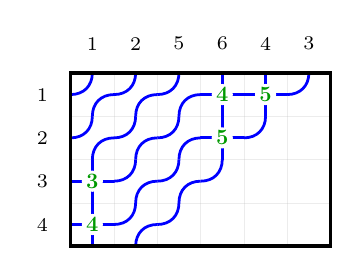
\begin{tikzpicture}[scale=0.55]
  \draw[lightgray, very thin, opacity=0.3] (0,2) -- (6,2);
  \draw[lightgray, very thin, opacity=0.3] (0,3) -- (6,3);
  \draw[lightgray, very thin, opacity=0.3] (0,4) -- (6,4);
  \draw[lightgray, very thin, opacity=0.3] (0,5) -- (6,5);
  \draw[lightgray, very thin, opacity=0.3] (0,6) -- (6,6);
  \draw[lightgray, very thin, opacity=0.3] (0,2) -- (0,6);
  \draw[lightgray, very thin, opacity=0.3] (1,2) -- (1,6);
  \draw[lightgray, very thin, opacity=0.3] (2,2) -- (2,6);
  \draw[lightgray, very thin, opacity=0.3] (3,2) -- (3,6);
  \draw[lightgray, very thin, opacity=0.3] (4,2) -- (4,6);
  \draw[lightgray, very thin, opacity=0.3] (5,2) -- (5,6);
  \draw[lightgray, very thin, opacity=0.3] (6,2) -- (6,6);
  \draw[blue, line width=1.0pt] (0,5.5) .. controls (0.3,5.5) and (0.5,5.7) .. (0.5,6);
  \draw[blue, line width=1.0pt] (0.5,5) .. controls (0.5,5.3) and (0.7,5.5) .. (1,5.5);
  \draw[blue, line width=1.0pt] (1,5.5) .. controls (1.3,5.5) and (1.5,5.7) .. (1.5,6);
  \draw[blue, line width=1.0pt] (1.5,5) .. controls (1.5,5.3) and (1.7,5.5) .. (2,5.5);
  \draw[blue, line width=1.0pt] (2,5.5) .. controls (2.3,5.5) and (2.5,5.7) .. (2.5,6);
  \draw[blue, line width=1.0pt] (2.5,5) .. controls (2.5,5.3) and (2.7,5.5) .. (3,5.5);
  \draw[blue, line width=1.0pt, line cap=round] (3,5.5) -- (4,5.5);
  \draw[blue, line width=1.0pt, line cap=round] (3.5,5) -- (3.5,6);
  \draw[blue, line width=1.0pt, line cap=round] (4,5.5) -- (5,5.5);
  \draw[blue, line width=1.0pt, line cap=round] (4.5,5) -- (4.5,6);
  \draw[blue, line width=1.0pt] (5,5.5) .. controls (5.3,5.5) and (5.5,5.7) .. (5.5,6);
  \draw[blue, line width=1.0pt] (0,4.5) .. controls (0.3,4.5) and (0.5,4.7) .. (0.5,5);
  \draw[blue, line width=1.0pt] (0.5,4) .. controls (0.5,4.3) and (0.7,4.5) .. (1,4.5);
  \draw[blue, line width=1.0pt] (1,4.5) .. controls (1.3,4.5) and (1.5,4.7) .. (1.5,5);
  \draw[blue, line width=1.0pt] (1.5,4) .. controls (1.5,4.3) and (1.7,4.5) .. (2,4.5);
  \draw[blue, line width=1.0pt] (2,4.5) .. controls (2.3,4.5) and (2.5,4.7) .. (2.5,5);
  \draw[blue, line width=1.0pt] (2.5,4) .. controls (2.5,4.3) and (2.7,4.5) .. (3,4.5);
  \draw[blue, line width=1.0pt, line cap=round] (3,4.5) -- (4,4.5);
  \draw[blue, line width=1.0pt, line cap=round] (3.5,4) -- (3.5,5);
  \draw[blue, line width=1.0pt] (4,4.5) .. controls (4.3,4.5) and (4.5,4.7) .. (4.5,5);
  \draw[blue, line width=1.0pt, line cap=round] (0,3.5) -- (1,3.5);
  \draw[blue, line width=1.0pt, line cap=round] (0.5,3) -- (0.5,4);
  \draw[blue, line width=1.0pt] (1,3.5) .. controls (1.3,3.5) and (1.5,3.7) .. (1.5,4);
  \draw[blue, line width=1.0pt] (1.5,3) .. controls (1.5,3.3) and (1.7,3.5) .. (2,3.5);
  \draw[blue, line width=1.0pt] (2,3.5) .. controls (2.3,3.5) and (2.5,3.7) .. (2.5,4);
  \draw[blue, line width=1.0pt] (2.5,3) .. controls (2.5,3.3) and (2.7,3.5) .. (3,3.5);
  \draw[blue, line width=1.0pt] (3,3.5) .. controls (3.3,3.5) and (3.5,3.7) .. (3.5,4);
  \draw[blue, line width=1.0pt, line cap=round] (0,2.5) -- (1,2.5);
  \draw[blue, line width=1.0pt, line cap=round] (0.5,2) -- (0.5,3);
  \draw[blue, line width=1.0pt] (1,2.5) .. controls (1.3,2.5) and (1.5,2.7) .. (1.5,3);
  \draw[blue, line width=1.0pt] (1.5,2) .. controls (1.5,2.3) and (1.7,2.5) .. (2,2.5);
  \draw[blue, line width=1.0pt] (2,2.5) .. controls (2.3,2.5) and (2.5,2.7) .. (2.5,3);
  \node[font=\Large\bfseries, text=green!60!black, fill=white, inner sep=0.5pt, circle, transform shape] at (3.5,4.5) {5};
  \node[font=\Large\bfseries, text=green!60!black, fill=white, inner sep=0.5pt, circle, transform shape] at (4.5,5.5) {5};
  \node[font=\Large\bfseries, text=green!60!black, fill=white, inner sep=0.5pt, circle, transform shape] at (0.5,3.5) {3};
  \node[font=\Large\bfseries, text=green!60!black, fill=white, inner sep=0.5pt, circle, transform shape] at (3.5,5.5) {4};
  \node[font=\Large\bfseries, text=green!60!black, fill=white, inner sep=0.5pt, circle, transform shape] at (0.5,2.5) {4};
  \node[font=\scriptsize, text=black, anchor=south] at (0.5,6.3) {1};
  \node[font=\scriptsize, text=black, anchor=south] at (1.5,6.3) {2};
  \node[font=\scriptsize, text=black, anchor=south] at (2.5,6.3) {5};
  \node[font=\scriptsize, text=black, anchor=south] at (3.5,6.3) {6};
  \node[font=\scriptsize, text=black, anchor=south] at (4.5,6.3) {4};
  \node[font=\scriptsize, text=black, anchor=south] at (5.5,6.3) {3};
  \node[font=\scriptsize, text=black, anchor=east] at (-0.3,5.5) {1};
  \node[font=\scriptsize, text=black, anchor=east] at (-0.3,4.5) {2};
  \node[font=\scriptsize, text=black, anchor=east] at (-0.3,3.5) {3};
  \node[font=\scriptsize, text=black, anchor=east] at (-0.3,2.5) {4};
  \draw[black, line width=1.2000000000000002pt] (0,2) rectangle (6,6);
\end{tikzpicture}}}
  \\[1em]
  + & 
  \vcenter{\hbox{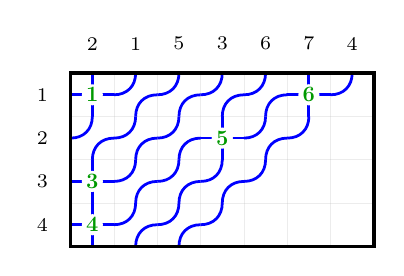
\begin{tikzpicture}[scale=0.55]
  \draw[lightgray, very thin, opacity=0.3] (0,3) -- (7,3);
  \draw[lightgray, very thin, opacity=0.3] (0,4) -- (7,4);
  \draw[lightgray, very thin, opacity=0.3] (0,5) -- (7,5);
  \draw[lightgray, very thin, opacity=0.3] (0,6) -- (7,6);
  \draw[lightgray, very thin, opacity=0.3] (0,7) -- (7,7);
  \draw[lightgray, very thin, opacity=0.3] (0,3) -- (0,7);
  \draw[lightgray, very thin, opacity=0.3] (1,3) -- (1,7);
  \draw[lightgray, very thin, opacity=0.3] (2,3) -- (2,7);
  \draw[lightgray, very thin, opacity=0.3] (3,3) -- (3,7);
  \draw[lightgray, very thin, opacity=0.3] (4,3) -- (4,7);
  \draw[lightgray, very thin, opacity=0.3] (5,3) -- (5,7);
  \draw[lightgray, very thin, opacity=0.3] (6,3) -- (6,7);
  \draw[lightgray, very thin, opacity=0.3] (7,3) -- (7,7);
  \draw[blue, line width=1.0pt, line cap=round] (0,6.5) -- (1,6.5);
  \draw[blue, line width=1.0pt, line cap=round] (0.5,6) -- (0.5,7);
  \draw[blue, line width=1.0pt] (1,6.5) .. controls (1.3,6.5) and (1.5,6.7) .. (1.5,7);
  \draw[blue, line width=1.0pt] (1.5,6) .. controls (1.5,6.3) and (1.7,6.5) .. (2,6.5);
  \draw[blue, line width=1.0pt] (2,6.5) .. controls (2.3,6.5) and (2.5,6.7) .. (2.5,7);
  \draw[blue, line width=1.0pt] (2.5,6) .. controls (2.5,6.3) and (2.7,6.5) .. (3,6.5);
  \draw[blue, line width=1.0pt] (3,6.5) .. controls (3.3,6.5) and (3.5,6.7) .. (3.5,7);
  \draw[blue, line width=1.0pt] (3.5,6) .. controls (3.5,6.3) and (3.7,6.5) .. (4,6.5);
  \draw[blue, line width=1.0pt] (4,6.5) .. controls (4.3,6.5) and (4.5,6.7) .. (4.5,7);
  \draw[blue, line width=1.0pt] (4.5,6) .. controls (4.5,6.3) and (4.7,6.5) .. (5,6.5);
  \draw[blue, line width=1.0pt, line cap=round] (5,6.5) -- (6,6.5);
  \draw[blue, line width=1.0pt, line cap=round] (5.5,6) -- (5.5,7);
  \draw[blue, line width=1.0pt] (6,6.5) .. controls (6.3,6.5) and (6.5,6.7) .. (6.5,7);
  \draw[blue, line width=1.0pt] (0,5.5) .. controls (0.3,5.5) and (0.5,5.7) .. (0.5,6);
  \draw[blue, line width=1.0pt] (0.5,5) .. controls (0.5,5.3) and (0.7,5.5) .. (1,5.5);
  \draw[blue, line width=1.0pt] (1,5.5) .. controls (1.3,5.5) and (1.5,5.7) .. (1.5,6);
  \draw[blue, line width=1.0pt] (1.5,5) .. controls (1.5,5.3) and (1.7,5.5) .. (2,5.5);
  \draw[blue, line width=1.0pt] (2,5.5) .. controls (2.3,5.5) and (2.5,5.7) .. (2.5,6);
  \draw[blue, line width=1.0pt] (2.5,5) .. controls (2.5,5.3) and (2.7,5.5) .. (3,5.5);
  \draw[blue, line width=1.0pt, line cap=round] (3,5.5) -- (4,5.5);
  \draw[blue, line width=1.0pt, line cap=round] (3.5,5) -- (3.5,6);
  \draw[blue, line width=1.0pt] (4,5.5) .. controls (4.3,5.5) and (4.5,5.7) .. (4.5,6);
  \draw[blue, line width=1.0pt] (4.5,5) .. controls (4.5,5.3) and (4.7,5.5) .. (5,5.5);
  \draw[blue, line width=1.0pt] (5,5.5) .. controls (5.3,5.5) and (5.5,5.7) .. (5.5,6);
  \draw[blue, line width=1.0pt, line cap=round] (0,4.5) -- (1,4.5);
  \draw[blue, line width=1.0pt, line cap=round] (0.5,4) -- (0.5,5);
  \draw[blue, line width=1.0pt] (1,4.5) .. controls (1.3,4.5) and (1.5,4.7) .. (1.5,5);
  \draw[blue, line width=1.0pt] (1.5,4) .. controls (1.5,4.3) and (1.7,4.5) .. (2,4.5);
  \draw[blue, line width=1.0pt] (2,4.5) .. controls (2.3,4.5) and (2.5,4.7) .. (2.5,5);
  \draw[blue, line width=1.0pt] (2.5,4) .. controls (2.5,4.3) and (2.7,4.5) .. (3,4.5);
  \draw[blue, line width=1.0pt] (3,4.5) .. controls (3.3,4.5) and (3.5,4.7) .. (3.5,5);
  \draw[blue, line width=1.0pt] (3.5,4) .. controls (3.5,4.3) and (3.7,4.5) .. (4,4.5);
  \draw[blue, line width=1.0pt] (4,4.5) .. controls (4.3,4.5) and (4.5,4.7) .. (4.5,5);
  \draw[blue, line width=1.0pt, line cap=round] (0,3.5) -- (1,3.5);
  \draw[blue, line width=1.0pt, line cap=round] (0.5,3) -- (0.5,4);
  \draw[blue, line width=1.0pt] (1,3.5) .. controls (1.3,3.5) and (1.5,3.7) .. (1.5,4);
  \draw[blue, line width=1.0pt] (1.5,3) .. controls (1.5,3.3) and (1.7,3.5) .. (2,3.5);
  \draw[blue, line width=1.0pt] (2,3.5) .. controls (2.3,3.5) and (2.5,3.7) .. (2.5,4);
  \draw[blue, line width=1.0pt] (2.5,3) .. controls (2.5,3.3) and (2.7,3.5) .. (3,3.5);
  \draw[blue, line width=1.0pt] (3,3.5) .. controls (3.3,3.5) and (3.5,3.7) .. (3.5,4);
  \node[font=\Large\bfseries, text=green!60!black, fill=white, inner sep=0.5pt, circle, transform shape] at (3.5,5.5) {5};
  \node[font=\Large\bfseries, text=green!60!black, fill=white, inner sep=0.5pt, circle, transform shape] at (0.5,4.5) {3};
  \node[font=\Large\bfseries, text=green!60!black, fill=white, inner sep=0.5pt, circle, transform shape] at (0.5,6.5) {1};
  \node[font=\Large\bfseries, text=green!60!black, fill=white, inner sep=0.5pt, circle, transform shape] at (5.5,6.5) {6};
  \node[font=\Large\bfseries, text=green!60!black, fill=white, inner sep=0.5pt, circle, transform shape] at (0.5,3.5) {4};
  \node[font=\scriptsize, text=black, anchor=south] at (0.5,7.3) {2};
  \node[font=\scriptsize, text=black, anchor=south] at (1.5,7.3) {1};
  \node[font=\scriptsize, text=black, anchor=south] at (2.5,7.3) {5};
  \node[font=\scriptsize, text=black, anchor=south] at (3.5,7.3) {3};
  \node[font=\scriptsize, text=black, anchor=south] at (4.5,7.3) {6};
  \node[font=\scriptsize, text=black, anchor=south] at (5.5,7.3) {7};
  \node[font=\scriptsize, text=black, anchor=south] at (6.5,7.3) {4};
  \node[font=\scriptsize, text=black, anchor=east] at (-0.3,6.5) {1};
  \node[font=\scriptsize, text=black, anchor=east] at (-0.3,5.5) {2};
  \node[font=\scriptsize, text=black, anchor=east] at (-0.3,4.5) {3};
  \node[font=\scriptsize, text=black, anchor=east] at (-0.3,3.5) {4};
  \draw[black, line width=1.2000000000000002pt] (0,3) rectangle (7,7);
\end{tikzpicture}}}
  +
  \vcenter{\hbox{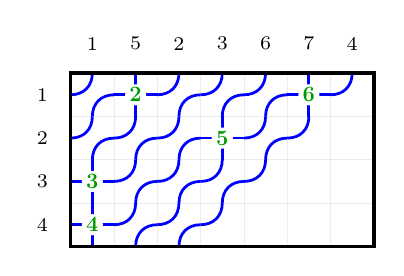
\begin{tikzpicture}[scale=0.55]
  \draw[lightgray, very thin, opacity=0.3] (0,3) -- (7,3);
  \draw[lightgray, very thin, opacity=0.3] (0,4) -- (7,4);
  \draw[lightgray, very thin, opacity=0.3] (0,5) -- (7,5);
  \draw[lightgray, very thin, opacity=0.3] (0,6) -- (7,6);
  \draw[lightgray, very thin, opacity=0.3] (0,7) -- (7,7);
  \draw[lightgray, very thin, opacity=0.3] (0,3) -- (0,7);
  \draw[lightgray, very thin, opacity=0.3] (1,3) -- (1,7);
  \draw[lightgray, very thin, opacity=0.3] (2,3) -- (2,7);
  \draw[lightgray, very thin, opacity=0.3] (3,3) -- (3,7);
  \draw[lightgray, very thin, opacity=0.3] (4,3) -- (4,7);
  \draw[lightgray, very thin, opacity=0.3] (5,3) -- (5,7);
  \draw[lightgray, very thin, opacity=0.3] (6,3) -- (6,7);
  \draw[lightgray, very thin, opacity=0.3] (7,3) -- (7,7);
  \draw[blue, line width=1.0pt] (0,6.5) .. controls (0.3,6.5) and (0.5,6.7) .. (0.5,7);
  \draw[blue, line width=1.0pt] (0.5,6) .. controls (0.5,6.3) and (0.7,6.5) .. (1,6.5);
  \draw[blue, line width=1.0pt, line cap=round] (1,6.5) -- (2,6.5);
  \draw[blue, line width=1.0pt, line cap=round] (1.5,6) -- (1.5,7);
  \draw[blue, line width=1.0pt] (2,6.5) .. controls (2.3,6.5) and (2.5,6.7) .. (2.5,7);
  \draw[blue, line width=1.0pt] (2.5,6) .. controls (2.5,6.3) and (2.7,6.5) .. (3,6.5);
  \draw[blue, line width=1.0pt] (3,6.5) .. controls (3.3,6.5) and (3.5,6.7) .. (3.5,7);
  \draw[blue, line width=1.0pt] (3.5,6) .. controls (3.5,6.3) and (3.7,6.5) .. (4,6.5);
  \draw[blue, line width=1.0pt] (4,6.5) .. controls (4.3,6.5) and (4.5,6.7) .. (4.5,7);
  \draw[blue, line width=1.0pt] (4.5,6) .. controls (4.5,6.3) and (4.7,6.5) .. (5,6.5);
  \draw[blue, line width=1.0pt, line cap=round] (5,6.5) -- (6,6.5);
  \draw[blue, line width=1.0pt, line cap=round] (5.5,6) -- (5.5,7);
  \draw[blue, line width=1.0pt] (6,6.5) .. controls (6.3,6.5) and (6.5,6.7) .. (6.5,7);
  \draw[blue, line width=1.0pt] (0,5.5) .. controls (0.3,5.5) and (0.5,5.7) .. (0.5,6);
  \draw[blue, line width=1.0pt] (0.5,5) .. controls (0.5,5.3) and (0.7,5.5) .. (1,5.5);
  \draw[blue, line width=1.0pt] (1,5.5) .. controls (1.3,5.5) and (1.5,5.7) .. (1.5,6);
  \draw[blue, line width=1.0pt] (1.5,5) .. controls (1.5,5.3) and (1.7,5.5) .. (2,5.5);
  \draw[blue, line width=1.0pt] (2,5.5) .. controls (2.3,5.5) and (2.5,5.7) .. (2.5,6);
  \draw[blue, line width=1.0pt] (2.5,5) .. controls (2.5,5.3) and (2.7,5.5) .. (3,5.5);
  \draw[blue, line width=1.0pt, line cap=round] (3,5.5) -- (4,5.5);
  \draw[blue, line width=1.0pt, line cap=round] (3.5,5) -- (3.5,6);
  \draw[blue, line width=1.0pt] (4,5.5) .. controls (4.3,5.5) and (4.5,5.7) .. (4.5,6);
  \draw[blue, line width=1.0pt] (4.5,5) .. controls (4.5,5.3) and (4.7,5.5) .. (5,5.5);
  \draw[blue, line width=1.0pt] (5,5.5) .. controls (5.3,5.5) and (5.5,5.7) .. (5.5,6);
  \draw[blue, line width=1.0pt, line cap=round] (0,4.5) -- (1,4.5);
  \draw[blue, line width=1.0pt, line cap=round] (0.5,4) -- (0.5,5);
  \draw[blue, line width=1.0pt] (1,4.5) .. controls (1.3,4.5) and (1.5,4.7) .. (1.5,5);
  \draw[blue, line width=1.0pt] (1.5,4) .. controls (1.5,4.3) and (1.7,4.5) .. (2,4.5);
  \draw[blue, line width=1.0pt] (2,4.5) .. controls (2.3,4.5) and (2.5,4.7) .. (2.5,5);
  \draw[blue, line width=1.0pt] (2.5,4) .. controls (2.5,4.3) and (2.7,4.5) .. (3,4.5);
  \draw[blue, line width=1.0pt] (3,4.5) .. controls (3.3,4.5) and (3.5,4.7) .. (3.5,5);
  \draw[blue, line width=1.0pt] (3.5,4) .. controls (3.5,4.3) and (3.7,4.5) .. (4,4.5);
  \draw[blue, line width=1.0pt] (4,4.5) .. controls (4.3,4.5) and (4.5,4.7) .. (4.5,5);
  \draw[blue, line width=1.0pt, line cap=round] (0,3.5) -- (1,3.5);
  \draw[blue, line width=1.0pt, line cap=round] (0.5,3) -- (0.5,4);
  \draw[blue, line width=1.0pt] (1,3.5) .. controls (1.3,3.5) and (1.5,3.7) .. (1.5,4);
  \draw[blue, line width=1.0pt] (1.5,3) .. controls (1.5,3.3) and (1.7,3.5) .. (2,3.5);
  \draw[blue, line width=1.0pt] (2,3.5) .. controls (2.3,3.5) and (2.5,3.7) .. (2.5,4);
  \draw[blue, line width=1.0pt] (2.5,3) .. controls (2.5,3.3) and (2.7,3.5) .. (3,3.5);
  \draw[blue, line width=1.0pt] (3,3.5) .. controls (3.3,3.5) and (3.5,3.7) .. (3.5,4);
  \node[font=\Large\bfseries, text=green!60!black, fill=white, inner sep=0.5pt, circle, transform shape] at (3.5,5.5) {5};
  \node[font=\Large\bfseries, text=green!60!black, fill=white, inner sep=0.5pt, circle, transform shape] at (1.5,6.5) {2};
  \node[font=\Large\bfseries, text=green!60!black, fill=white, inner sep=0.5pt, circle, transform shape] at (0.5,4.5) {3};
  \node[font=\Large\bfseries, text=green!60!black, fill=white, inner sep=0.5pt, circle, transform shape] at (5.5,6.5) {6};
  \node[font=\Large\bfseries, text=green!60!black, fill=white, inner sep=0.5pt, circle, transform shape] at (0.5,3.5) {4};
  \node[font=\scriptsize, text=black, anchor=south] at (0.5,7.3) {1};
  \node[font=\scriptsize, text=black, anchor=south] at (1.5,7.3) {5};
  \node[font=\scriptsize, text=black, anchor=south] at (2.5,7.3) {2};
  \node[font=\scriptsize, text=black, anchor=south] at (3.5,7.3) {3};
  \node[font=\scriptsize, text=black, anchor=south] at (4.5,7.3) {6};
  \node[font=\scriptsize, text=black, anchor=south] at (5.5,7.3) {7};
  \node[font=\scriptsize, text=black, anchor=south] at (6.5,7.3) {4};
  \node[font=\scriptsize, text=black, anchor=east] at (-0.3,6.5) {1};
  \node[font=\scriptsize, text=black, anchor=east] at (-0.3,5.5) {2};
  \node[font=\scriptsize, text=black, anchor=east] at (-0.3,4.5) {3};
  \node[font=\scriptsize, text=black, anchor=east] at (-0.3,3.5) {4};
  \draw[black, line width=1.2000000000000002pt] (0,3) rectangle (7,7);
\end{tikzpicture}}}
  +
  \vcenter{\hbox{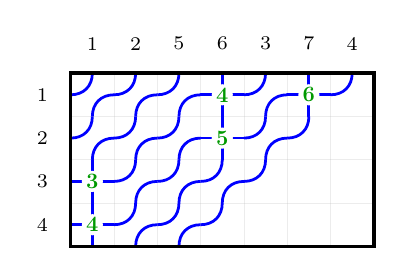
\begin{tikzpicture}[scale=0.55]
  \draw[lightgray, very thin, opacity=0.3] (0,3) -- (7,3);
  \draw[lightgray, very thin, opacity=0.3] (0,4) -- (7,4);
  \draw[lightgray, very thin, opacity=0.3] (0,5) -- (7,5);
  \draw[lightgray, very thin, opacity=0.3] (0,6) -- (7,6);
  \draw[lightgray, very thin, opacity=0.3] (0,7) -- (7,7);
  \draw[lightgray, very thin, opacity=0.3] (0,3) -- (0,7);
  \draw[lightgray, very thin, opacity=0.3] (1,3) -- (1,7);
  \draw[lightgray, very thin, opacity=0.3] (2,3) -- (2,7);
  \draw[lightgray, very thin, opacity=0.3] (3,3) -- (3,7);
  \draw[lightgray, very thin, opacity=0.3] (4,3) -- (4,7);
  \draw[lightgray, very thin, opacity=0.3] (5,3) -- (5,7);
  \draw[lightgray, very thin, opacity=0.3] (6,3) -- (6,7);
  \draw[lightgray, very thin, opacity=0.3] (7,3) -- (7,7);
  \draw[blue, line width=1.0pt] (0,6.5) .. controls (0.3,6.5) and (0.5,6.7) .. (0.5,7);
  \draw[blue, line width=1.0pt] (0.5,6) .. controls (0.5,6.3) and (0.7,6.5) .. (1,6.5);
  \draw[blue, line width=1.0pt] (1,6.5) .. controls (1.3,6.5) and (1.5,6.7) .. (1.5,7);
  \draw[blue, line width=1.0pt] (1.5,6) .. controls (1.5,6.3) and (1.7,6.5) .. (2,6.5);
  \draw[blue, line width=1.0pt] (2,6.5) .. controls (2.3,6.5) and (2.5,6.7) .. (2.5,7);
  \draw[blue, line width=1.0pt] (2.5,6) .. controls (2.5,6.3) and (2.7,6.5) .. (3,6.5);
  \draw[blue, line width=1.0pt, line cap=round] (3,6.5) -- (4,6.5);
  \draw[blue, line width=1.0pt, line cap=round] (3.5,6) -- (3.5,7);
  \draw[blue, line width=1.0pt] (4,6.5) .. controls (4.3,6.5) and (4.5,6.7) .. (4.5,7);
  \draw[blue, line width=1.0pt] (4.5,6) .. controls (4.5,6.3) and (4.7,6.5) .. (5,6.5);
  \draw[blue, line width=1.0pt, line cap=round] (5,6.5) -- (6,6.5);
  \draw[blue, line width=1.0pt, line cap=round] (5.5,6) -- (5.5,7);
  \draw[blue, line width=1.0pt] (6,6.5) .. controls (6.3,6.5) and (6.5,6.7) .. (6.5,7);
  \draw[blue, line width=1.0pt] (0,5.5) .. controls (0.3,5.5) and (0.5,5.7) .. (0.5,6);
  \draw[blue, line width=1.0pt] (0.5,5) .. controls (0.5,5.3) and (0.7,5.5) .. (1,5.5);
  \draw[blue, line width=1.0pt] (1,5.5) .. controls (1.3,5.5) and (1.5,5.7) .. (1.5,6);
  \draw[blue, line width=1.0pt] (1.5,5) .. controls (1.5,5.3) and (1.7,5.5) .. (2,5.5);
  \draw[blue, line width=1.0pt] (2,5.5) .. controls (2.3,5.5) and (2.5,5.7) .. (2.5,6);
  \draw[blue, line width=1.0pt] (2.5,5) .. controls (2.5,5.3) and (2.7,5.5) .. (3,5.5);
  \draw[blue, line width=1.0pt, line cap=round] (3,5.5) -- (4,5.5);
  \draw[blue, line width=1.0pt, line cap=round] (3.5,5) -- (3.5,6);
  \draw[blue, line width=1.0pt] (4,5.5) .. controls (4.3,5.5) and (4.5,5.7) .. (4.5,6);
  \draw[blue, line width=1.0pt] (4.5,5) .. controls (4.5,5.3) and (4.7,5.5) .. (5,5.5);
  \draw[blue, line width=1.0pt] (5,5.5) .. controls (5.3,5.5) and (5.5,5.7) .. (5.5,6);
  \draw[blue, line width=1.0pt, line cap=round] (0,4.5) -- (1,4.5);
  \draw[blue, line width=1.0pt, line cap=round] (0.5,4) -- (0.5,5);
  \draw[blue, line width=1.0pt] (1,4.5) .. controls (1.3,4.5) and (1.5,4.7) .. (1.5,5);
  \draw[blue, line width=1.0pt] (1.5,4) .. controls (1.5,4.3) and (1.7,4.5) .. (2,4.5);
  \draw[blue, line width=1.0pt] (2,4.5) .. controls (2.3,4.5) and (2.5,4.7) .. (2.5,5);
  \draw[blue, line width=1.0pt] (2.5,4) .. controls (2.5,4.3) and (2.7,4.5) .. (3,4.5);
  \draw[blue, line width=1.0pt] (3,4.5) .. controls (3.3,4.5) and (3.5,4.7) .. (3.5,5);
  \draw[blue, line width=1.0pt] (3.5,4) .. controls (3.5,4.3) and (3.7,4.5) .. (4,4.5);
  \draw[blue, line width=1.0pt] (4,4.5) .. controls (4.3,4.5) and (4.5,4.7) .. (4.5,5);
  \draw[blue, line width=1.0pt, line cap=round] (0,3.5) -- (1,3.5);
  \draw[blue, line width=1.0pt, line cap=round] (0.5,3) -- (0.5,4);
  \draw[blue, line width=1.0pt] (1,3.5) .. controls (1.3,3.5) and (1.5,3.7) .. (1.5,4);
  \draw[blue, line width=1.0pt] (1.5,3) .. controls (1.5,3.3) and (1.7,3.5) .. (2,3.5);
  \draw[blue, line width=1.0pt] (2,3.5) .. controls (2.3,3.5) and (2.5,3.7) .. (2.5,4);
  \draw[blue, line width=1.0pt] (2.5,3) .. controls (2.5,3.3) and (2.7,3.5) .. (3,3.5);
  \draw[blue, line width=1.0pt] (3,3.5) .. controls (3.3,3.5) and (3.5,3.7) .. (3.5,4);
  \node[font=\Large\bfseries, text=green!60!black, fill=white, inner sep=0.5pt, circle, transform shape] at (3.5,5.5) {5};
  \node[font=\Large\bfseries, text=green!60!black, fill=white, inner sep=0.5pt, circle, transform shape] at (0.5,4.5) {3};
  \node[font=\Large\bfseries, text=green!60!black, fill=white, inner sep=0.5pt, circle, transform shape] at (3.5,6.5) {4};
  \node[font=\Large\bfseries, text=green!60!black, fill=white, inner sep=0.5pt, circle, transform shape] at (5.5,6.5) {6};
  \node[font=\Large\bfseries, text=green!60!black, fill=white, inner sep=0.5pt, circle, transform shape] at (0.5,3.5) {4};
  \node[font=\scriptsize, text=black, anchor=south] at (0.5,7.3) {1};
  \node[font=\scriptsize, text=black, anchor=south] at (1.5,7.3) {2};
  \node[font=\scriptsize, text=black, anchor=south] at (2.5,7.3) {5};
  \node[font=\scriptsize, text=black, anchor=south] at (3.5,7.3) {6};
  \node[font=\scriptsize, text=black, anchor=south] at (4.5,7.3) {3};
  \node[font=\scriptsize, text=black, anchor=south] at (5.5,7.3) {7};
  \node[font=\scriptsize, text=black, anchor=south] at (6.5,7.3) {4};
  \node[font=\scriptsize, text=black, anchor=east] at (-0.3,6.5) {1};
  \node[font=\scriptsize, text=black, anchor=east] at (-0.3,5.5) {2};
  \node[font=\scriptsize, text=black, anchor=east] at (-0.3,4.5) {3};
  \node[font=\scriptsize, text=black, anchor=east] at (-0.3,3.5) {4};
  \draw[black, line width=1.2000000000000002pt] (0,3) rectangle (7,7);
\end{tikzpicture}}}
\end{align*}


\end{example}


% \subsection{Generating the RC graph ring}
% \newcommand{\BRCC}{\overline{\BRC}}
% % multiplying by empty row ordering
% We enlarge the module $\BRC$ to include bounded RC graphs $R$ with $\hr(R)=n$ that do not necessarily satisfy the condition that $\maxd(\wof{R})\leq n$, only that $R$ has at most $n$ rows. We denote this larger module by $\BRCC$. For $(R, p)\in \BRCC$, define $(R, p)^T\in \BRC$ by $(R^T,\maxd(\wof{R}^{-1}))$. We may define an associative product on $\BRCC$ by
% $$(R_1, p)\spadesuit(R_2,q) = \mathtt{sz}_{p+q}(((R_1, p)^T\sqcupplus (R_2, q)^T)^T)$$
% where $\mathtt{sz}_n:\BRCC\to \BRCC$ is defined on basis elements by 
% $$\mathtt{sz}_n(R, m) = \begin{cases}(R, n) & \text{if } i\leq n\text{ for all }(i, j)\in R\\
% 0 & \text{otherwise}\end{cases}$$
\subsection{Proof of the Littlewood-Richardson rule for the dual Schubert basis}


\begin{definition}
Define a map $\Xi:\BRC\to \dcoma$ by
$$\Xi(R) = \dsch_{\wof{R}}^{\hr(R)}$$
and $\omega:\BRC\to\dcoma$ by
$$\omega(R) = [\wtt(R)]$$

Let $\mathcal{R}$  be the subring of $\BRC$ generated by the single-row RC graphs $\mathtt{row}(i)$ for $i\geq 0$. Let $a$ be a sequence of elements of a ring indexed by the nonnegative integers. For a permutation $w$ and an integer $n\geq \maxd(w)$, define a function $\dsch_w^n(a)$ by
$$\dsch_w^n(a) = \sum_{\alpha} d_{\alpha, w}^n a_{\alpha_1} \cdots a_{\alpha_n}$$
where the sum is over all weak compositions $\alpha$ of length $n$, and $d_{\alpha, w}^n$ is the coefficient of $\alpha$ in $\dsch_w^n\in\dcoma$.
\end{definition}

\begin{proposition}
We have that the elements
$$\dsch_w^n(\mathtt{row})$$
for integers $n\geq 0$ and $w$ that ranges over all permutations in $S_\infty$ with $n\geq \maxd(w)$ form a $\mathbb{Z}$-basis of $\mathcal{R}$, and $\alpha:\mathcal{R}\to \dcoma$ is an isomorphism of graded rings.
\end{proposition}
\begin{proof}
Since $\alpha(\dsch_w(\mathtt{row})) = \dsch_w^n\in \dcoma$, the elements $\dsch_w^n(\mathtt{row})$ are linearly independent. Given that the images form a basis of $\dcoma$, they must also span $\mathcal{R}$ since $\dcoma$ is a free algebra, and hence there is a homomorphism backwards $\dcoma\to \mathcal{R}$ sending $[i]\mapsto \mathtt{row}(i)$ which is necessarily surjective. Thus, the elements $\dsch_w^n(\mathtt{row})$ form a $\mathbb{Z}$-basis of $\mathcal{R}$.
\end{proof}

\begin{definition}
Let $\Omega$ be the $\mathbb{Z}$-submodule of $\BRC$ generated by the RC graphs $R_1-R_2$ such that $\wof{R_1}=\wof{R_2}$ and $\hr(R_1)=\hr(R_2)$.
\end{definition}

\begin{lemma}
$\Omega$ is a two-sided ideal of $\BRC$.
\end{lemma}
\begin{proof}
  The fact that $\Omega$ is a left ideal follows from the fact that a product $R\sqcupplus R_1$ is uniquely determines by $R\sqcupplus \mathrm{empty}(\hr(R_1))$ and $R_1$, and the contribution of $R_1$ is precisely that it replaces the last $\hr(R_1)$ rows of each term. In particular, precisely the same $\hr(R)$ occur in precisely the same number of terms, to which $\shup^{\hr(R)}R_1$ is added as the last $\hr(R_1)$ rows. It follows that $R\sqcupplus R_1 - R\sqcupplus R_2$ is a linear combination of terms of the form $R_1' - R_2'$ such that $\hr(R_1') = \hr(R_2')$ and $\wof{R_1'} = \wof{R_2'}$, and $\Omega$ is a left ideal.

  The fact that $\Omega$ is a right ideal follows from the fact that a product $R_1\sqcupplus R$ is uniquely determined by $R_1\sqcupplus \mathrm{empty}(\hr(R))$ and $R$, and the contribution of $R$ is precisely that it replaces the last $\hr(R)$ rows of each term. In particular, precisely the same $\hr(R)$ occur in precisely the same number of terms, to which $\shup^{\hr(R)}R$ is added as the last $\hr(R)$ rows. It follows that $R_1\sqcupplus R - R_2\sqcupplus R$ is a linear combination of terms of the form $R_1' - R_2'$ such that $\hr(R_1') = \hr(R_2')$ and $\wof{R_1'} = \wof{R_2'}$, and $\Omega$ is a right ideal.
\end{proof}

\begin{theorem} \label{theorem:semidirect}
  We have that $\alpha:\BRC\to \dcoma$ is a surjective homomorphism of rings with kernel $\Omega$, and the homomorphism $\iota:\dcoma\to\BRC$ sending $[i]\mapsto \mathtt{row}(i)$ is a right inverse to $\alpha$. In particular, $\BRC\cong \dcoma\ltimes \Omega$ as rings.
\end{theorem}
\begin{proof}
  We have an exact sequence
$$0\to \Omega\to \BRC\to \dcoma\to 0$$
where the map $\BRC\to \dcoma$ is $\alpha$. We have a homomorphism $\iota:\dcoma\to \BRC$ sending $[i]\mapsto \mathtt{row}(i)$ inducing an isomorphism on $\mathcal{R}$, and the composition $\dcoma\to \BRC\to \dcoma$ is the identity since $\alpha(\mathtt{row}(i)) = [i]$. Since $\Omega$ is a two-sided ideal, we can conclude that $\alpha$ is in fact a homomorphism of rings. Since $\BRC = \mathcal{R}\oplus \Omega$, by virtue of the fact that the sequence is split, and $\mathcal{R}\cong \dcoma$, we have $\BRC\cong \dcoma\ltimes \Omega$ as rings.
\end{proof}

\begin{proposition}
Let $[c]$ be a weak composition of length $n$. Then
$$[c] = \sum_{\substack{w\in S_\infty\\\maxd(w)\leq n}}\#{R\in \RC_n(w)\mid wtt(R)=c} \dsch_{\wof{R}}^n$$
\end{proposition}


\begin{definition}
Given RC graphs $U\in \RC_p(u)$ and $V\in\RC_q(v)$ and a permutation $w$, define
$$d_{U, V}^w = \#\{R\in \RC(w, p + q): \clp^p(R)=U,\trm^p(R)=V\}$$
\end{definition}

\begin{proof}[Proof of Theorem \ref{theorem:LR}]
For any choice of RC graphs $U_1,U_2\in \RC_p(u)$ and $V_1,V_2\in\RC_q(v)$ and a permutation $w$, we have $\alpha(U_1) = \alpha(U_2)$ and $\alpha(V_1)=\alpha(V_2)$, so that $\alpha(U_1)\alpha(V_1) = \alpha(U_2)\alpha(V_2)$. We have
$$U_1\sqcupplus V_1 = \sum_{\clp^p(R)=U_1,\trm^p(R)=V_1} R$$
Applying $\alpha$, we then have that
$$\dsch_u^p\sqcupplus \dsch_v^q = \alpha(U_1)\sqcupplus\alpha(V_1) = \alpha(U_1\sqcupplus V_1) = \sum_{\clp^p(R)=U_1,\trm^p(R)=V_1} \alpha(R)=\sum_{\clp^p(R)=U_1,\trm^p(R)=V_1} \dsch_{\wof{R}}^{p+q}$$
The coefficient of $\dsch_w^{p+q}$ in this product is precisely $d_{U_1, V_1}^w=d_{U_2, V_2}^w$ by definition, and we have the result.
\end{proof}

% Let $R$ be an RC graph with $\wof{R}=w$ and $\hr(R)=n$. Then for any $m\leq n$,
% $$\dsch_w^n = \alpha(\clp^m(R))\alpha(\trm^m(R)) - \sum_{\substack{\clp^m(R')=\clp^m(R)\\\trm^m(R')=\trm^m(R)\\R'\neq R}} \alpha(R')$$

% $n=4$

% $$\dsch_w^4 = \alpha(\clp^2(R))\alpha(\trm^2(R)) - \sum_{R'}\alpha(\clp^1(R))\alpha(\trm^1(R'))$$

% $$\dsch_w^m = \sum_i(-1)^{i-1}\sum_{\substack{\clp^{\left\lfloor \frac m{2^{i}}\right\rfloor}(R')=\clp^{\left\lfloor \frac m{2^{i}}\right\rfloor}(R)\\\trm^{\left\lfloor \frac m{2^{i}}\right\rfloor}(R')=\trm^{\left\lfloor \frac m{2^{i}}\right\rfloor}(R)\\\trm^{\left\lfloor \frac m{2^{i+1}}\right\rfloor}(R')\neq\trm^{\left\lfloor \frac m{2^{i+1}}\right\rfloor}(R)}} \alpha(\clp^{\left\lfloor \frac m{2^i}\right\rfloor}(R))\alpha(\trm^{\left\lfloor \frac m{2^i}\right\rfloor}(R'))$$

% Suppose $D\in \dcoma$ satisfies
% $$D = \sum_{w} c_w \dsch_w^n$$
% Then
% $$D = \sum_{w} c_w \wtt(\dsch_w^n(\mathtt{row}))$$

\section{The ring of RC graph crystals}\label{section:crystals}

\subsection{Little bumps and the crystal action on RC graphs}

\begin{definition}[Crystal action on RC graphs, highest weights, extremal weights] \label{definition:crystal}
Following Morse and Schilling \cite{morse2016crystal}, who defined an $A_{\ell-1}$-crystal structure on reduced factorizations of a permutation $w$, and the adaptation to RC graphs by Assaf and Schilling \cite{assaf2018demazure}, we equip $\RC(w)$ with Kashiwara raising and lowering operators $e_i, f_i$ for $i\geq 1$. The operator pair $(e_i, f_i)$ acts only on rows $i$ and $i+1$ of an RC graph $R$, viewed as adjacent factors in the corresponding reduced factorization.

The action is governed by a bracketing procedure on the column indices appearing in rows $i$ and $i+1$. Process the entries of row $i$ in decreasing order of column index: for each column $b$ in row $i$, pair it with the smallest column $a>b$ appearing in row $i+1$ that has not yet been paired in an earlier step; if no such $a$ exists, $b$ is left unpaired. Let $R_i(R)$ denote the set of unpaired column indices in row $i$, and $L_i(R)$ the set of unpaired column indices in row $i+1$.

If $R_i(R)$ is nonempty, $f_i(R)$ is obtained by removing the smallest unpaired entry $b\in R_i(R)$ from row $i$ and inserting an entry into row $i+1$ at the largest column $b' < b$ such that $b'$ does not already appear in row $i+1$; if $R_i(R) = \emptyset$ or no such $b'$ exists, $f_i(R) = \emptyset$. Dually, if $L_i(R)$ is nonempty, $e_i(R)$ is obtained by removing the largest unpaired entry $a\in L_i(R)$ from row $i+1$ and inserting an entry into row $i$ at the smallest column $a' > a$ such that $a'$ does not already appear in row $i$; if $L_i(R) = \emptyset$ or no such $a'$ exists, $e_i(R) = \emptyset$.

The \emph{weight} of $R$ as an element of the crystal is simply $\wtt(R)$, the row weight itself. A \emph{highest weight} element is an RC graph $R$ with $e_i(R) = \emptyset$ for all $i\geq 1$. Every $R\in \RC(w)$ corresponds to a unique highest weight element $\mathbb{Y}(R)$, which can always be obtained by greedily applying available $e_i$ until none apply.The \emph{Demazure crystal} $\mathrm{Dem}(R)$ generated by a highest weight $\mathbb{Y}(R)$ is the closure of $\{\mathbb{Y}(R)\}$ under the operators $\{f_i^k : i\geq 1, k\geq 0\}$ subject to the Demazure truncation rule of \cite{assaf2018demazure}. The \emph{extremal weight} $\mathrm{extwt}(R)$ of $R$ is the weak composition that is the lexicographically smallest weight of any element of $\mathrm{Dem}(R)$.
\end{definition}

The significance of this elaborate structure is the following.
\begin{theorem} \label{theorem:keykey}
If $A\in\BRC$ is such that $\mathrm{extwt}(A) = a$, then
$$\kappa_a = \sum_{R\in\mathrm{Dem}(A)} x^{\wtt(R)}$$
\end{theorem}

It will be advantageous to have an alternative, crystal-friendly definition of the map $\zeromap$ for the purposes of proving results about key polynomials.

\begin{definition}[Little bumps]
  Given a reduced word $a_1\cdots a_m$ for a permutation $w$ and an index $1\leq p\leq m$, the \emph{Little bump} $\ltb_p(a_1\cdots a_m)$ is defined recursively as follows. If $a_p>1$, replace $a_p$ with $a_p-1$, and if $a_p=1$ then instead replace all $a_q$ with $q\neq p$ with $a_q+1$. Denote the new word by $a_1'\cdots a_m'$. If this resulting word is reduced, we are done. Otherwise, there is a unique index $j\neq p$ such that the word obtained by deleting $a_j'$ from the new word is reduced by the deletion property of Coxeter groups. We then define
  $$\ltb_p(a_1\cdots a_m) = \ltb_j(a_1'\cdots a_m')$$
\end{definition}

\begin{definition}
Define a function $\lmap:\BRC^0(n)\to\BRC(n+1)$ as follows. Assume $n=\maxd(\wof{R})$, and suppose $\rtt_R(i, j) = (n, n + 1)$, where $i < n$. Set 
$$R'= (R\setminus \{(i, j)\})\cup \{(n,1)\}$$
Then define
$$\lmap(R) = (\ins{n-1}{i} R')\setminus\{(n, 1)\}$$
which we assign height $n+1$. Then define $\lzeromap:\BRC^0(n)\to \BRC(n-1)$ by iterating $\lmap$ and stopping as soon as the result has $\maxd(\wof{R})\leq n-1$, then reducing the number of rows to $n-1$.
\end{definition}

\begin{proposition} \label{proposition:little_bump}
  Let $(R, n)\in \BRC^0(n)$ be a bounded RC graph such that $\maxd(\wof{R}) = n$. Suppose 
  $$\mathrm{word}(R) = a_1 a_2 \cdots a_k$$ 
  and 
  $$\mathrm{seq}(R) = r_1 r_2 \cdots r_k$$ 
  suppose $\rtt_R(i,j)=(n,n+1)$, and let $p$ be the index such that $r_p=i$ and $r_p + j - 1 = a_p$. Then
  $$\mathrm{word}(\lmap(R)) = \ltb_{p}(\mathrm{word}(R))$$
\end{proposition}
\begin{proof}
Consider the biword
$$\begin{matrix}
r_1& r_2& \cdots & r_{p-1} & r_p & r_{p+1} & \cdots & r_k\\
a_1& a_2& \cdots & a_{p-1} & a_p & a_{p+1} & \cdots & a_k
\end{matrix}$$
The first deletion yields
$$\begin{matrix}
r_1& r_2& \cdots & r_{p-1} &  r_{p+1} & \cdots & r_k& n\\
a_1& a_2& \cdots & a_{p-1} &  a_{p+1} & \cdots & a_k& n
\end{matrix}$$
Necessarily, we must have $a_p > 1$. To see this, note that if we have $a_p=1$, then we would have $r_p=1$ by the compatible sequence condition. The only way for position $(1,1)$ in an RC graph to be the final right descent is if it is the unique right descent. By assumption, that descent would have to be $n$, so that $n=1$. In that case, however, it would not be possible for the last row to be empty, which is included in the hypotheses of the proposition.

We must also have that $r_p < a_p$, because there is a sequence of chute moves involving this crossing that moves it to position $(n, 1)$ by \cite[Theorem~3.7]{bbrc}. Assume first that $p = k$. Then the insertion algorithm will insert $a_p - 1=n-1$ into row $r_k$. If this word is reduced, then we are done, and this clearly coincides with the Little bump. If it is not reduced, the descent $n-1$ occurs somewhere to the left, say at position $j$. The insertion algorithm would delete this letter then try to insert another one. Recursively, this is the same as applying $\lmap$ to the biword obtained by removing all letters after position $j$ and then reinserting them afterwards. By the inductive hypothesis, this coincides with applying the Little bump at position $j$, which would indeed be the next step in the recursion of applying the Little bump at position $k$. Thus, the two coincide by induction.
\end{proof}



We invoke the following theorem of Hamaker and Young.

\begin{theorem}[{\cite[Theorem~4.4]{hamaker2014relating}}] \label{theorem:littlecrystal}
Let $\mathrm{w}$ be a reduced word for a permutation $w\in S_\infty$. Then
$$Q(\mathrm{w}) = Q(\ltb_p(\mathrm{w}))$$
for any valid $p$.
\end{theorem}


\begin{proposition} \label{proposition:zeroequal}
  We have that
$$\lzeromap:\RC(w, n)^0\to \bigcup_{w\downvar{n} w'}\RC(w', n-1)$$ 
	is an isomorphism of crystal graphs.
\end{proposition}
\begin{proof}
The fact that this is a weight-preserving bijection follows directly from repeated application of \cite[Lemma~7]{little2003combinatorial}, which states that the Little bump on the last descent realizes the Lascoux-Sch\"utzenberger transition formula. The crystal isomorphism follows from Theorem \ref{theorem:littlecrystal}.
\end{proof}

\begin{theorem} \label{theorem:zerocrystal}
We have the equality $\lzeromap=\zeromap$.
\end{theorem}
\begin{proof}
Let $R$ be a bounded RC graph, say with permutation $w$, with $r$ rows and last descent $r$ such that row $r$ is empty. We prove this by induction on $\ell(w)$ as well as on $s - r$, where $s>r$ is the maximal index such that $w(r)>w(s)$. If $s=r+1$, then the definitions of the two maps are identical. 

% Otherwise, we quote the following formula:
% $$\sch_w(x) = \sch_w(x_1, \ldots, x_{r-1}, 0) + x_r\partial^r(\sch_w(x))(x_1,\ldots,x_r,0)$$
% We model the second term as follows. 
By the exchange property of Coxeter groups, there is a unique pair $(i,j)$ such that $\rtt_R(i, j) = (r, r+1)$. Set
$$R' = R\setminus\{(i,j)\}$$
and assume that $\hr(R') = r+1$. By the inductive hypothesis, we have $\lzeromap(R') = \zeromap(R')$. We have thus established that $\lzeromap$ and $\zeromap$ induce the same bijection between $\RC(ws_r)^0$ and 
$$\bigcup_{ws_r\downvar{r+1} w'}\RC(w')$$
Inspection of both algorithms reveals that the removal of this crossing and the subsequent reinsertion in the first step of both algorithms is precisely the same, and holding this fixed then applying the inductive hypothesis yields the result.
\end{proof}

\begin{corollary} \label{corollary:crystaliso}
For any bounded RC graph $R$ and any $i\geq 1$, we have 
$$\zeromap(e_i(R)) = e_i(\zeromap(R))$$
and
$$\zeromap(f_i(R)) = f_i(\zeromap(R))$$
whenever the left-hand sides are defined.
\end{corollary}

\subsection{The dual key basis and the ring of RC graph crystals}

\begin{definition}[The dual key basis]
  For a weak composition $a$ of length $n$, define $\kappa_a^*\in \dcoma_n$ to be the unique element such that $\langle \kappa_a^*, \kappa_b\rangle = \delta_{a,b}$ for all weak compositions $b$.
\end{definition}

% We invoke the following result of Reiner and Shimozono.


% where $\mathrm{Dem}_{\RC}(a)$ is the set of RC graphs $R$ such that $\mathrm{extwt}(R) = a$. In particular, the Demazure crystal $\mathrm{Dem}(R)$ is precisely the set of RC graphs $R'$ such that $\mathbb{Y}(R') = \mathbb{Y}(R)$ and $\mathrm{extwt}(R') = \mathrm{extwt}(R)$, so that the above formula is equivalent to the following result of Reiner and Shimozono.

% \begin{theorem}[{\cite[Theorem~5(3)]{reiner1995key}}] \label{theorem:keykey}
%   For a weak composition $a$ of length $n$, we have
%   $$\kappa_a = \sum_{\mathrm{rev}(\mathbf{r})\sim_{\mathrm{CK}} \mathrm{key}(a)\atop b\mbox{ is }a{-compatible}} x^b$$
% \end{theorem}


\begin{theorem} \label{theorem:keyformula}
  Let $c$ be a weak composition. Then dual key polynomial $\kappa^*_c$ is equal to
$$\kappa^*_c = \sum_{R=\mathbb{Y}(R)\atop\mathrm{extwt}(R)=c} \dsch_{\wof{R}}^{\hr(R)}$$
\end{theorem}
\begin{proof}
  The statement of the theorem is equivalent to Lascoux and Sch\"utzenberger's formula for Schubert polynomials in terms of key polynomials through Theorem \ref{theorem:keykey}.
\end{proof}

\begin{proposition}
Let $c$ be a weak composition of length $p$. Let $\RC_{\mathbb{Y}}(c)$ be the set of RC graphs $R$ with $\wtt(R) = c$ such that $\mathrm{word}(\mathbb{Y}(R))$ is minimal in lexicographical order among all RC graphs $R'$ such that $\mathrm{extwt}(R) = \mathrm{extwt}(R')$. Then
$$[c] = \sum_{R\in\RC_{\mathbb{Y}}(c)} \kappa_{\mathrm{extwt}(\mathbb{Y}(R))}^*$$
\end{proposition}

\begin{definition}[The submodule $\Theta\subseteq \BRC$]
  Let $\Theta$ be the $\mathbb{Z}$-submodule of $\BRC$ generated by the elements $R_1-R_2$ such that $\mathbb{Y}(R_1)=\mathbb{Y}(R_2)$.

\end{definition}

\begin{lemma}
  $\Theta$ is a two-sided ideal of $\BRC$.
\end{lemma}
\begin{proof}
  The fact that $\Theta$ is a left ideal follows from the fact that the products $R\sqcupplus R_1$ and $R\sqcupplus R_2$ have the same first $\hr(R)$ rows, and the rows below are simply shifts of $R_1$ and $R_2$. Since the crystal raising/lowering operators act directly on adjacent rows, the same crystal operators will apply to the rows below, so that $R\sqcupplus R_1$ and $R\sqcupplus R_2$ have the same crystal structure in the trailing rows. In passing to highest weights $\mathbb{Y}(R\sqcupplus R_1)$ and $\mathbb{Y}(R\sqcupplus R_2)$, we may pass through the partial highest weights $R\sqcupplus Y(R_1) = R\sqcupplus Y(R_2)$, so that in particular the highest weights of the bijectively corresponding terms of $R\sqcupplus R_1$ and $R\sqcupplus R_2$ are the same.
  
  %, so that $R\sqcupplus R_1 - R\sqcupplus R_2$ is a linear combination of terms of the form $R_1' - R_2'$ such that $\mathbb{Y}(R_1') = \mathbb{Y}(R_2')$, and $\Theta$ is a left ideal.

  To prove that $\Theta$ is a right ideal, the same argument applies, but we must invoke Corollary \ref{corollary:crystaliso} to guarantee that the crystals remain isomorphic as needed.
\end{proof}

\begin{lemma}
  The homomorphism $\alpha:\BRC\to\dcoma$ factors through the quotient $\BRC/\Theta$.
\end{lemma}
\begin{proof}
This is because the generators of $\Theta$ are all in $\Omega$.
\end{proof}

\begin{definition}
For a composition $a$, define  an element $K_a\in\BRC/\Theta$ by
$$K_a =\sum_{R\in\mathrm{Dem}_{\RC}(a)\atop R=\mathbb{Y}(R)} R$$
\end{definition}

\begin{proposition}
The elements $K_a\in\BRC/\Theta$ form an additive basis of a subring isomorphic to $\dcoma$ under the homomorphism $\alpha:\BRC/\Theta\to \dcoma$, and 
$$\alpha(K_a) = \kappa_a^*$$
\end{proposition}
\begin{proof}
The last statement is simply Theorem \ref{theorem:keyformula}. The $K_a$ actually consist of pairwise disjoint sets of RC graphs, the set of all such is clearly independent. To show that they span a subring, consider the homomorphism $\alpha:\BRC/\Theta\to \dcoma$. We have that $\alpha(K_a)=\kappa_a^*$, and since these are linearly independent, it follows that the kernel of $\alpha$ intersects trivially with the span of the $K_a$. Since $\alpha$ is a homomorphism, it follows that $\alpha$ is injective on the span of the $K_a$, and since 
$$\alpha(K_a)\sqcupplus\alpha(K_b) = \kappa_a^*\sqcupplus\kappa_b^*=\sum_{c}k_{ab}^c\,\kappa_c^*=\sum k_{a,b}^c\,\alpha(K_c),$$ 
it follows that $K_a\sqcupplus K_b$ is a linear combination of the $K_c$, so the span of the $K_a$ is closed under multiplication, so that $\alpha$ is an isomorphism and we are done.
\end{proof}

\begin{proof}[Proof of Theorem \ref{theorem:LRkey}]
  The coefficient of $K_c$ in $K_a\sqcupplus K_b$ is the same as the coefficient of $\kappa_c^*$ in $\kappa_a^*\sqcupplus\kappa_b^*$, which is $k_{a,b}^c$ by definition. Since each of the summands of $K_c$ that are Demazure crystals of RC graphs are distinct from the summands of any other key element and each other, we need only consider one of the summands to read off the coefficient. The result follows.
\end{proof}

\begin{example}[Computing $\kappa_a^*\sqcupplus\kappa_b^*$ for $a=(0,1,2)$, $b=(0,1,0,2)$]\label{example:LRkey}
Let $a=(0,1,2)$ (a $3$-row composition) and $b=(0,1,0,2)$ (a $4$-row composition), so $p=3$, $q=4$, and $p+q=7$. We illustrate the coefficient $k_{a,b}^c$ for $c=(0,0,0,1,2,0,3)$.

The permutation $w_c$ whose principal RC graph has Demazure crystal highest weight $c$ is
$$w_c = (1,2,3,5,7,4,10,6,8,9).$$
The key element $K_c$ is the sum of all $7$-row RC graphs whose Demazure crystal highest weight equals $c$. Among these, exactly two satisfy $\clp^3(R)\in\mathcal{C}_a$ and $\trm^3(R)\in\mathcal{C}_b$:

\begin{figure}[h]
\centering
\begin{tabular}{cc}
$R_1$ & $R_2$ \\[4pt]
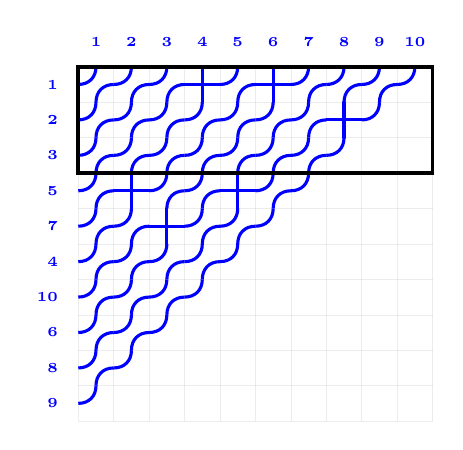
\begin{tikzpicture}[scale=0.45]
  \draw[lightgray, very thin, opacity=0.3] (10.3,0) -- (0.3,0);
  \draw[lightgray, very thin, opacity=0.3] (10.3,0) -- (10.3,10);
  \draw[lightgray, very thin, opacity=0.3] (10.3,1) -- (0.3,1);
  \draw[lightgray, very thin, opacity=0.3] (9.3,0) -- (9.3,10);
  \draw[lightgray, very thin, opacity=0.3] (10.3,2) -- (0.3,2);
  \draw[lightgray, very thin, opacity=0.3] (8.3,0) -- (8.3,10);
  \draw[lightgray, very thin, opacity=0.3] (10.3,3) -- (0.3,3);
  \draw[lightgray, very thin, opacity=0.3] (7.3,0) -- (7.3,10);
  \draw[lightgray, very thin, opacity=0.3] (10.3,4) -- (0.3,4);
  \draw[lightgray, very thin, opacity=0.3] (6.3,0) -- (6.3,10);
  \draw[lightgray, very thin, opacity=0.3] (10.3,5) -- (0.3,5);
  \draw[lightgray, very thin, opacity=0.3] (5.3,0) -- (5.3,10);
  \draw[lightgray, very thin, opacity=0.3] (10.3,6) -- (0.3,6);
  \draw[lightgray, very thin, opacity=0.3] (4.3,0) -- (4.3,10);
  \draw[lightgray, very thin, opacity=0.3] (10.3,7) -- (0.3,7);
  \draw[lightgray, very thin, opacity=0.3] (3.3,0) -- (3.3,10);
  \draw[lightgray, very thin, opacity=0.3] (10.3,8) -- (0.3,8);
  \draw[lightgray, very thin, opacity=0.3] (2.3,0) -- (2.3,10);
  \draw[lightgray, very thin, opacity=0.3] (10.3,9) -- (0.3,9);
  \draw[lightgray, very thin, opacity=0.3] (1.3,0) -- (1.3,10);
  \draw[lightgray, very thin, opacity=0.3] (10.3,10) -- (0.3,10);
  \draw[lightgray, very thin, opacity=0.3] (0.3,0) -- (0.3,10);
  \draw[blue, line width=1.125pt] (0.3,9.5) .. controls (0.6,9.5) and (0.8,9.7) .. (0.8,10);
  \draw[blue, line width=1.125pt] (0.8,9) .. controls (0.8,9.3) and (1,9.5) .. (1.3,9.5);
  \draw[blue, line width=1.125pt] (1.3,9.5) .. controls (1.6,9.5) and (1.8,9.7) .. (1.8,10);
  \draw[blue, line width=1.125pt] (1.8,9) .. controls (1.8,9.3) and (2,9.5) .. (2.3,9.5);
  \draw[blue, line width=1.125pt] (2.3,9.5) .. controls (2.6,9.5) and (2.8,9.7) .. (2.8,10);
  \draw[blue, line width=1.125pt] (2.8,9) .. controls (2.8,9.3) and (3,9.5) .. (3.3,9.5);
  \draw[blue, line width=1.125pt, line cap=round] (3.3,9.5) -- (4.3,9.5);
  \draw[blue, line width=1.125pt, line cap=round] (3.8,9) -- (3.8,10);
  \draw[blue, line width=1.125pt] (4.3,9.5) .. controls (4.6,9.5) and (4.8,9.7) .. (4.8,10);
  \draw[blue, line width=1.125pt] (4.8,9) .. controls (4.8,9.3) and (5,9.5) .. (5.3,9.5);
  \draw[blue, line width=1.125pt, line cap=round] (5.3,9.5) -- (6.3,9.5);
  \draw[blue, line width=1.125pt, line cap=round] (5.8,9) -- (5.8,10);
  \draw[blue, line width=1.125pt] (6.3,9.5) .. controls (6.6,9.5) and (6.8,9.7) .. (6.8,10);
  \draw[blue, line width=1.125pt] (6.8,9) .. controls (6.8,9.3) and (7,9.5) .. (7.3,9.5);
  \draw[blue, line width=1.125pt] (7.3,9.5) .. controls (7.6,9.5) and (7.8,9.7) .. (7.8,10);
  \draw[blue, line width=1.125pt] (7.8,9) .. controls (7.8,9.3) and (8,9.5) .. (8.3,9.5);
  \draw[blue, line width=1.125pt] (8.3,9.5) .. controls (8.6,9.5) and (8.8,9.7) .. (8.8,10);
  \draw[blue, line width=1.125pt] (8.8,9) .. controls (8.8,9.3) and (9,9.5) .. (9.3,9.5);
  \draw[blue, line width=1.125pt] (9.3,9.5) .. controls (9.6,9.5) and (9.8,9.7) .. (9.8,10);
  \draw[blue, line width=1.125pt] (0.3,8.5) .. controls (0.6,8.5) and (0.8,8.7) .. (0.8,9);
  \draw[blue, line width=1.125pt] (0.8,8) .. controls (0.8,8.3) and (1,8.5) .. (1.3,8.5);
  \draw[blue, line width=1.125pt] (1.3,8.5) .. controls (1.6,8.5) and (1.8,8.7) .. (1.8,9);
  \draw[blue, line width=1.125pt] (1.8,8) .. controls (1.8,8.3) and (2,8.5) .. (2.3,8.5);
  \draw[blue, line width=1.125pt] (2.3,8.5) .. controls (2.6,8.5) and (2.8,8.7) .. (2.8,9);
  \draw[blue, line width=1.125pt] (2.8,8) .. controls (2.8,8.3) and (3,8.5) .. (3.3,8.5);
  \draw[blue, line width=1.125pt] (3.3,8.5) .. controls (3.6,8.5) and (3.8,8.7) .. (3.8,9);
  \draw[blue, line width=1.125pt] (3.8,8) .. controls (3.8,8.3) and (4,8.5) .. (4.3,8.5);
  \draw[blue, line width=1.125pt] (4.3,8.5) .. controls (4.6,8.5) and (4.8,8.7) .. (4.8,9);
  \draw[blue, line width=1.125pt] (4.8,8) .. controls (4.8,8.3) and (5,8.5) .. (5.3,8.5);
  \draw[blue, line width=1.125pt] (5.3,8.5) .. controls (5.6,8.5) and (5.8,8.7) .. (5.8,9);
  \draw[blue, line width=1.125pt] (5.8,8) .. controls (5.8,8.3) and (6,8.5) .. (6.3,8.5);
  \draw[blue, line width=1.125pt] (6.3,8.5) .. controls (6.6,8.5) and (6.8,8.7) .. (6.8,9);
  \draw[blue, line width=1.125pt] (6.8,8) .. controls (6.8,8.3) and (7,8.5) .. (7.3,8.5);
  \draw[blue, line width=1.125pt, line cap=round] (7.3,8.5) -- (8.3,8.5);
  \draw[blue, line width=1.125pt, line cap=round] (7.8,8) -- (7.8,9);
  \draw[blue, line width=1.125pt] (8.3,8.5) .. controls (8.6,8.5) and (8.8,8.7) .. (8.8,9);
  \draw[blue, line width=1.125pt] (0.3,7.5) .. controls (0.6,7.5) and (0.8,7.7) .. (0.8,8);
  \draw[blue, line width=1.125pt] (0.8,7) .. controls (0.8,7.3) and (1,7.5) .. (1.3,7.5);
  \draw[blue, line width=1.125pt] (1.3,7.5) .. controls (1.6,7.5) and (1.8,7.7) .. (1.8,8);
  \draw[blue, line width=1.125pt] (1.8,7) .. controls (1.8,7.3) and (2,7.5) .. (2.3,7.5);
  \draw[blue, line width=1.125pt] (2.3,7.5) .. controls (2.6,7.5) and (2.8,7.7) .. (2.8,8);
  \draw[blue, line width=1.125pt] (2.8,7) .. controls (2.8,7.3) and (3,7.5) .. (3.3,7.5);
  \draw[blue, line width=1.125pt] (3.3,7.5) .. controls (3.6,7.5) and (3.8,7.7) .. (3.8,8);
  \draw[blue, line width=1.125pt] (3.8,7) .. controls (3.8,7.3) and (4,7.5) .. (4.3,7.5);
  \draw[blue, line width=1.125pt] (4.3,7.5) .. controls (4.6,7.5) and (4.8,7.7) .. (4.8,8);
  \draw[blue, line width=1.125pt] (4.8,7) .. controls (4.8,7.3) and (5,7.5) .. (5.3,7.5);
  \draw[blue, line width=1.125pt] (5.3,7.5) .. controls (5.6,7.5) and (5.8,7.7) .. (5.8,8);
  \draw[blue, line width=1.125pt] (5.8,7) .. controls (5.8,7.3) and (6,7.5) .. (6.3,7.5);
  \draw[blue, line width=1.125pt] (6.3,7.5) .. controls (6.6,7.5) and (6.8,7.7) .. (6.8,8);
  \draw[blue, line width=1.125pt] (6.8,7) .. controls (6.8,7.3) and (7,7.5) .. (7.3,7.5);
  \draw[blue, line width=1.125pt] (7.3,7.5) .. controls (7.6,7.5) and (7.8,7.7) .. (7.8,8);
  \draw[blue, line width=1.125pt] (0.3,6.5) .. controls (0.6,6.5) and (0.8,6.7) .. (0.8,7);
  \draw[blue, line width=1.125pt] (0.8,6) .. controls (0.8,6.3) and (1,6.5) .. (1.3,6.5);
  \draw[blue, line width=1.125pt, line cap=round] (1.3,6.5) -- (2.3,6.5);
  \draw[blue, line width=1.125pt, line cap=round] (1.8,6) -- (1.8,7);
  \draw[blue, line width=1.125pt] (2.3,6.5) .. controls (2.6,6.5) and (2.8,6.7) .. (2.8,7);
  \draw[blue, line width=1.125pt] (2.8,6) .. controls (2.8,6.3) and (3,6.5) .. (3.3,6.5);
  \draw[blue, line width=1.125pt] (3.3,6.5) .. controls (3.6,6.5) and (3.8,6.7) .. (3.8,7);
  \draw[blue, line width=1.125pt] (3.8,6) .. controls (3.8,6.3) and (4,6.5) .. (4.3,6.5);
  \draw[blue, line width=1.125pt, line cap=round] (4.3,6.5) -- (5.3,6.5);
  \draw[blue, line width=1.125pt, line cap=round] (4.8,6) -- (4.8,7);
  \draw[blue, line width=1.125pt] (5.3,6.5) .. controls (5.6,6.5) and (5.8,6.7) .. (5.8,7);
  \draw[blue, line width=1.125pt] (5.8,6) .. controls (5.8,6.3) and (6,6.5) .. (6.3,6.5);
  \draw[blue, line width=1.125pt] (6.3,6.5) .. controls (6.6,6.5) and (6.8,6.7) .. (6.8,7);
  \draw[blue, line width=1.125pt] (0.3,5.5) .. controls (0.6,5.5) and (0.8,5.7) .. (0.8,6);
  \draw[blue, line width=1.125pt] (0.8,5) .. controls (0.8,5.3) and (1,5.5) .. (1.3,5.5);
  \draw[blue, line width=1.125pt] (1.3,5.5) .. controls (1.6,5.5) and (1.8,5.7) .. (1.8,6);
  \draw[blue, line width=1.125pt] (1.8,5) .. controls (1.8,5.3) and (2,5.5) .. (2.3,5.5);
  \draw[blue, line width=1.125pt, line cap=round] (2.3,5.5) -- (3.3,5.5);
  \draw[blue, line width=1.125pt, line cap=round] (2.8,5) -- (2.8,6);
  \draw[blue, line width=1.125pt] (3.3,5.5) .. controls (3.6,5.5) and (3.8,5.7) .. (3.8,6);
  \draw[blue, line width=1.125pt] (3.8,5) .. controls (3.8,5.3) and (4,5.5) .. (4.3,5.5);
  \draw[blue, line width=1.125pt] (4.3,5.5) .. controls (4.6,5.5) and (4.8,5.7) .. (4.8,6);
  \draw[blue, line width=1.125pt] (4.8,5) .. controls (4.8,5.3) and (5,5.5) .. (5.3,5.5);
  \draw[blue, line width=1.125pt] (5.3,5.5) .. controls (5.6,5.5) and (5.8,5.7) .. (5.8,6);
  \draw[blue, line width=1.125pt] (0.3,4.5) .. controls (0.6,4.5) and (0.8,4.7) .. (0.8,5);
  \draw[blue, line width=1.125pt] (0.8,4) .. controls (0.8,4.3) and (1,4.5) .. (1.3,4.5);
  \draw[blue, line width=1.125pt] (1.3,4.5) .. controls (1.6,4.5) and (1.8,4.7) .. (1.8,5);
  \draw[blue, line width=1.125pt] (1.8,4) .. controls (1.8,4.3) and (2,4.5) .. (2.3,4.5);
  \draw[blue, line width=1.125pt] (2.3,4.5) .. controls (2.6,4.5) and (2.8,4.7) .. (2.8,5);
  \draw[blue, line width=1.125pt] (2.8,4) .. controls (2.8,4.3) and (3,4.5) .. (3.3,4.5);
  \draw[blue, line width=1.125pt] (3.3,4.5) .. controls (3.6,4.5) and (3.8,4.7) .. (3.8,5);
  \draw[blue, line width=1.125pt] (3.8,4) .. controls (3.8,4.3) and (4,4.5) .. (4.3,4.5);
  \draw[blue, line width=1.125pt] (4.3,4.5) .. controls (4.6,4.5) and (4.8,4.7) .. (4.8,5);
  \draw[blue, line width=1.125pt] (0.3,3.5) .. controls (0.6,3.5) and (0.8,3.7) .. (0.8,4);
  \draw[blue, line width=1.125pt] (0.8,3) .. controls (0.8,3.3) and (1,3.5) .. (1.3,3.5);
  \draw[blue, line width=1.125pt] (1.3,3.5) .. controls (1.6,3.5) and (1.8,3.7) .. (1.8,4);
  \draw[blue, line width=1.125pt] (1.8,3) .. controls (1.8,3.3) and (2,3.5) .. (2.3,3.5);
  \draw[blue, line width=1.125pt] (2.3,3.5) .. controls (2.6,3.5) and (2.8,3.7) .. (2.8,4);
  \draw[blue, line width=1.125pt] (2.8,3) .. controls (2.8,3.3) and (3,3.5) .. (3.3,3.5);
  \draw[blue, line width=1.125pt] (3.3,3.5) .. controls (3.6,3.5) and (3.8,3.7) .. (3.8,4);
  \draw[blue, line width=1.125pt] (0.3,2.5) .. controls (0.6,2.5) and (0.8,2.7) .. (0.8,3);
  \draw[blue, line width=1.125pt] (0.8,2) .. controls (0.8,2.3) and (1,2.5) .. (1.3,2.5);
  \draw[blue, line width=1.125pt] (1.3,2.5) .. controls (1.6,2.5) and (1.8,2.7) .. (1.8,3);
  \draw[blue, line width=1.125pt] (1.8,2) .. controls (1.8,2.3) and (2,2.5) .. (2.3,2.5);
  \draw[blue, line width=1.125pt] (2.3,2.5) .. controls (2.6,2.5) and (2.8,2.7) .. (2.8,3);
  \draw[blue, line width=1.125pt] (0.3,1.5) .. controls (0.6,1.5) and (0.8,1.7) .. (0.8,2);
  \draw[blue, line width=1.125pt] (0.8,1) .. controls (0.8,1.3) and (1,1.5) .. (1.3,1.5);
  \draw[blue, line width=1.125pt] (1.3,1.5) .. controls (1.6,1.5) and (1.8,1.7) .. (1.8,2);
  \draw[blue, line width=1.125pt] (0.3,0.5) .. controls (0.6,0.5) and (0.8,0.7) .. (0.8,1);
  \node[font=\tiny\bfseries, text=blue, anchor=south] at (0.8,10.3) {1};
  \node[font=\tiny\bfseries, text=blue, anchor=south] at (1.8,10.3) {2};
  \node[font=\tiny\bfseries, text=blue, anchor=south] at (2.8,10.3) {3};
  \node[font=\tiny\bfseries, text=blue, anchor=south] at (3.8,10.3) {4};
  \node[font=\tiny\bfseries, text=blue, anchor=south] at (4.8,10.3) {5};
  \node[font=\tiny\bfseries, text=blue, anchor=south] at (5.8,10.3) {6};
  \node[font=\tiny\bfseries, text=blue, anchor=south] at (6.8,10.3) {7};
  \node[font=\tiny\bfseries, text=blue, anchor=south] at (7.8,10.3) {8};
  \node[font=\tiny\bfseries, text=blue, anchor=south] at (8.8,10.3) {9};
  \node[font=\tiny\bfseries, text=blue, anchor=south] at (9.8,10.3) {10};
  \node[font=\tiny\bfseries, text=blue, anchor=east] at (0,9.5) {1};
  \node[font=\tiny\bfseries, text=blue, anchor=east] at (0,8.5) {2};
  \node[font=\tiny\bfseries, text=blue, anchor=east] at (0,7.5) {3};
  \node[font=\tiny\bfseries, text=blue, anchor=east] at (0,6.5) {5};
  \node[font=\tiny\bfseries, text=blue, anchor=east] at (0,5.5) {7};
  \node[font=\tiny\bfseries, text=blue, anchor=east] at (0,4.5) {4};
  \node[font=\tiny\bfseries, text=blue, anchor=east] at (0,3.5) {10};
  \node[font=\tiny\bfseries, text=blue, anchor=east] at (0,2.5) {6};
  \node[font=\tiny\bfseries, text=blue, anchor=east] at (0,1.5) {8};
  \node[font=\tiny\bfseries, text=blue, anchor=east] at (0,0.5) {9};
  \draw[black, line width=1.35pt] (10.3,7) rectangle (0.3,10);
\end{tikzpicture}
&
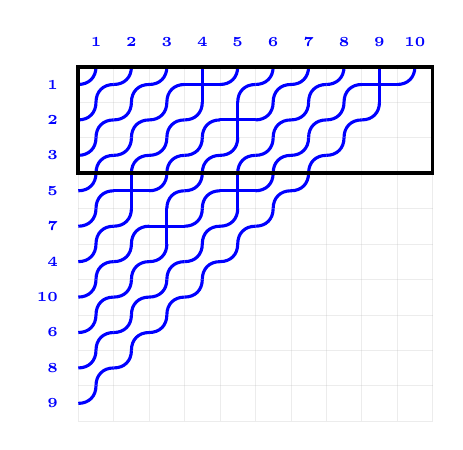
\begin{tikzpicture}[scale=0.45]
  \draw[lightgray, very thin, opacity=0.3] (10.3,0) -- (0.3,0);
  \draw[lightgray, very thin, opacity=0.3] (10.3,0) -- (10.3,10);
  \draw[lightgray, very thin, opacity=0.3] (10.3,1) -- (0.3,1);
  \draw[lightgray, very thin, opacity=0.3] (9.3,0) -- (9.3,10);
  \draw[lightgray, very thin, opacity=0.3] (10.3,2) -- (0.3,2);
  \draw[lightgray, very thin, opacity=0.3] (8.3,0) -- (8.3,10);
  \draw[lightgray, very thin, opacity=0.3] (10.3,3) -- (0.3,3);
  \draw[lightgray, very thin, opacity=0.3] (7.3,0) -- (7.3,10);
  \draw[lightgray, very thin, opacity=0.3] (10.3,4) -- (0.3,4);
  \draw[lightgray, very thin, opacity=0.3] (6.3,0) -- (6.3,10);
  \draw[lightgray, very thin, opacity=0.3] (10.3,5) -- (0.3,5);
  \draw[lightgray, very thin, opacity=0.3] (5.3,0) -- (5.3,10);
  \draw[lightgray, very thin, opacity=0.3] (10.3,6) -- (0.3,6);
  \draw[lightgray, very thin, opacity=0.3] (4.3,0) -- (4.3,10);
  \draw[lightgray, very thin, opacity=0.3] (10.3,7) -- (0.3,7);
  \draw[lightgray, very thin, opacity=0.3] (3.3,0) -- (3.3,10);
  \draw[lightgray, very thin, opacity=0.3] (10.3,8) -- (0.3,8);
  \draw[lightgray, very thin, opacity=0.3] (2.3,0) -- (2.3,10);
  \draw[lightgray, very thin, opacity=0.3] (10.3,9) -- (0.3,9);
  \draw[lightgray, very thin, opacity=0.3] (1.3,0) -- (1.3,10);
  \draw[lightgray, very thin, opacity=0.3] (10.3,10) -- (0.3,10);
  \draw[lightgray, very thin, opacity=0.3] (0.3,0) -- (0.3,10);
  \draw[blue, line width=1.125pt] (0.3,9.5) .. controls (0.6,9.5) and (0.8,9.7) .. (0.8,10);
  \draw[blue, line width=1.125pt] (0.8,9) .. controls (0.8,9.3) and (1,9.5) .. (1.3,9.5);
  \draw[blue, line width=1.125pt] (1.3,9.5) .. controls (1.6,9.5) and (1.8,9.7) .. (1.8,10);
  \draw[blue, line width=1.125pt] (1.8,9) .. controls (1.8,9.3) and (2,9.5) .. (2.3,9.5);
  \draw[blue, line width=1.125pt] (2.3,9.5) .. controls (2.6,9.5) and (2.8,9.7) .. (2.8,10);
  \draw[blue, line width=1.125pt] (2.8,9) .. controls (2.8,9.3) and (3,9.5) .. (3.3,9.5);
  \draw[blue, line width=1.125pt, line cap=round] (3.3,9.5) -- (4.3,9.5);
  \draw[blue, line width=1.125pt, line cap=round] (3.8,9) -- (3.8,10);
  \draw[blue, line width=1.125pt] (4.3,9.5) .. controls (4.6,9.5) and (4.8,9.7) .. (4.8,10);
  \draw[blue, line width=1.125pt] (4.8,9) .. controls (4.8,9.3) and (5,9.5) .. (5.3,9.5);
  \draw[blue, line width=1.125pt] (5.3,9.5) .. controls (5.6,9.5) and (5.8,9.7) .. (5.8,10);
  \draw[blue, line width=1.125pt] (5.8,9) .. controls (5.8,9.3) and (6,9.5) .. (6.3,9.5);
  \draw[blue, line width=1.125pt] (6.3,9.5) .. controls (6.6,9.5) and (6.8,9.7) .. (6.8,10);
  \draw[blue, line width=1.125pt] (6.8,9) .. controls (6.8,9.3) and (7,9.5) .. (7.3,9.5);
  \draw[blue, line width=1.125pt] (7.3,9.5) .. controls (7.6,9.5) and (7.8,9.7) .. (7.8,10);
  \draw[blue, line width=1.125pt] (7.8,9) .. controls (7.8,9.3) and (8,9.5) .. (8.3,9.5);
  \draw[blue, line width=1.125pt, line cap=round] (8.3,9.5) -- (9.3,9.5);
  \draw[blue, line width=1.125pt, line cap=round] (8.8,9) -- (8.8,10);
  \draw[blue, line width=1.125pt] (9.3,9.5) .. controls (9.6,9.5) and (9.8,9.7) .. (9.8,10);
  \draw[blue, line width=1.125pt] (0.3,8.5) .. controls (0.6,8.5) and (0.8,8.7) .. (0.8,9);
  \draw[blue, line width=1.125pt] (0.8,8) .. controls (0.8,8.3) and (1,8.5) .. (1.3,8.5);
  \draw[blue, line width=1.125pt] (1.3,8.5) .. controls (1.6,8.5) and (1.8,8.7) .. (1.8,9);
  \draw[blue, line width=1.125pt] (1.8,8) .. controls (1.8,8.3) and (2,8.5) .. (2.3,8.5);
  \draw[blue, line width=1.125pt] (2.3,8.5) .. controls (2.6,8.5) and (2.8,8.7) .. (2.8,9);
  \draw[blue, line width=1.125pt] (2.8,8) .. controls (2.8,8.3) and (3,8.5) .. (3.3,8.5);
  \draw[blue, line width=1.125pt] (3.3,8.5) .. controls (3.6,8.5) and (3.8,8.7) .. (3.8,9);
  \draw[blue, line width=1.125pt] (3.8,8) .. controls (3.8,8.3) and (4,8.5) .. (4.3,8.5);
  \draw[blue, line width=1.125pt, line cap=round] (4.3,8.5) -- (5.3,8.5);
  \draw[blue, line width=1.125pt, line cap=round] (4.8,8) -- (4.8,9);
  \draw[blue, line width=1.125pt] (5.3,8.5) .. controls (5.6,8.5) and (5.8,8.7) .. (5.8,9);
  \draw[blue, line width=1.125pt] (5.8,8) .. controls (5.8,8.3) and (6,8.5) .. (6.3,8.5);
  \draw[blue, line width=1.125pt] (6.3,8.5) .. controls (6.6,8.5) and (6.8,8.7) .. (6.8,9);
  \draw[blue, line width=1.125pt] (6.8,8) .. controls (6.8,8.3) and (7,8.5) .. (7.3,8.5);
  \draw[blue, line width=1.125pt] (7.3,8.5) .. controls (7.6,8.5) and (7.8,8.7) .. (7.8,9);
  \draw[blue, line width=1.125pt] (7.8,8) .. controls (7.8,8.3) and (8,8.5) .. (8.3,8.5);
  \draw[blue, line width=1.125pt] (8.3,8.5) .. controls (8.6,8.5) and (8.8,8.7) .. (8.8,9);
  \draw[blue, line width=1.125pt] (0.3,7.5) .. controls (0.6,7.5) and (0.8,7.7) .. (0.8,8);
  \draw[blue, line width=1.125pt] (0.8,7) .. controls (0.8,7.3) and (1,7.5) .. (1.3,7.5);
  \draw[blue, line width=1.125pt] (1.3,7.5) .. controls (1.6,7.5) and (1.8,7.7) .. (1.8,8);
  \draw[blue, line width=1.125pt] (1.8,7) .. controls (1.8,7.3) and (2,7.5) .. (2.3,7.5);
  \draw[blue, line width=1.125pt] (2.3,7.5) .. controls (2.6,7.5) and (2.8,7.7) .. (2.8,8);
  \draw[blue, line width=1.125pt] (2.8,7) .. controls (2.8,7.3) and (3,7.5) .. (3.3,7.5);
  \draw[blue, line width=1.125pt] (3.3,7.5) .. controls (3.6,7.5) and (3.8,7.7) .. (3.8,8);
  \draw[blue, line width=1.125pt] (3.8,7) .. controls (3.8,7.3) and (4,7.5) .. (4.3,7.5);
  \draw[blue, line width=1.125pt] (4.3,7.5) .. controls (4.6,7.5) and (4.8,7.7) .. (4.8,8);
  \draw[blue, line width=1.125pt] (4.8,7) .. controls (4.8,7.3) and (5,7.5) .. (5.3,7.5);
  \draw[blue, line width=1.125pt] (5.3,7.5) .. controls (5.6,7.5) and (5.8,7.7) .. (5.8,8);
  \draw[blue, line width=1.125pt] (5.8,7) .. controls (5.8,7.3) and (6,7.5) .. (6.3,7.5);
  \draw[blue, line width=1.125pt] (6.3,7.5) .. controls (6.6,7.5) and (6.8,7.7) .. (6.8,8);
  \draw[blue, line width=1.125pt] (6.8,7) .. controls (6.8,7.3) and (7,7.5) .. (7.3,7.5);
  \draw[blue, line width=1.125pt] (7.3,7.5) .. controls (7.6,7.5) and (7.8,7.7) .. (7.8,8);
  \draw[blue, line width=1.125pt] (0.3,6.5) .. controls (0.6,6.5) and (0.8,6.7) .. (0.8,7);
  \draw[blue, line width=1.125pt] (0.8,6) .. controls (0.8,6.3) and (1,6.5) .. (1.3,6.5);
  \draw[blue, line width=1.125pt, line cap=round] (1.3,6.5) -- (2.3,6.5);
  \draw[blue, line width=1.125pt, line cap=round] (1.8,6) -- (1.8,7);
  \draw[blue, line width=1.125pt] (2.3,6.5) .. controls (2.6,6.5) and (2.8,6.7) .. (2.8,7);
  \draw[blue, line width=1.125pt] (2.8,6) .. controls (2.8,6.3) and (3,6.5) .. (3.3,6.5);
  \draw[blue, line width=1.125pt] (3.3,6.5) .. controls (3.6,6.5) and (3.8,6.7) .. (3.8,7);
  \draw[blue, line width=1.125pt] (3.8,6) .. controls (3.8,6.3) and (4,6.5) .. (4.3,6.5);
  \draw[blue, line width=1.125pt, line cap=round] (4.3,6.5) -- (5.3,6.5);
  \draw[blue, line width=1.125pt, line cap=round] (4.8,6) -- (4.8,7);
  \draw[blue, line width=1.125pt] (5.3,6.5) .. controls (5.6,6.5) and (5.8,6.7) .. (5.8,7);
  \draw[blue, line width=1.125pt] (5.8,6) .. controls (5.8,6.3) and (6,6.5) .. (6.3,6.5);
  \draw[blue, line width=1.125pt] (6.3,6.5) .. controls (6.6,6.5) and (6.8,6.7) .. (6.8,7);
  \draw[blue, line width=1.125pt] (0.3,5.5) .. controls (0.6,5.5) and (0.8,5.7) .. (0.8,6);
  \draw[blue, line width=1.125pt] (0.8,5) .. controls (0.8,5.3) and (1,5.5) .. (1.3,5.5);
  \draw[blue, line width=1.125pt] (1.3,5.5) .. controls (1.6,5.5) and (1.8,5.7) .. (1.8,6);
  \draw[blue, line width=1.125pt] (1.8,5) .. controls (1.8,5.3) and (2,5.5) .. (2.3,5.5);
  \draw[blue, line width=1.125pt, line cap=round] (2.3,5.5) -- (3.3,5.5);
  \draw[blue, line width=1.125pt, line cap=round] (2.8,5) -- (2.8,6);
  \draw[blue, line width=1.125pt] (3.3,5.5) .. controls (3.6,5.5) and (3.8,5.7) .. (3.8,6);
  \draw[blue, line width=1.125pt] (3.8,5) .. controls (3.8,5.3) and (4,5.5) .. (4.3,5.5);
  \draw[blue, line width=1.125pt] (4.3,5.5) .. controls (4.6,5.5) and (4.8,5.7) .. (4.8,6);
  \draw[blue, line width=1.125pt] (4.8,5) .. controls (4.8,5.3) and (5,5.5) .. (5.3,5.5);
  \draw[blue, line width=1.125pt] (5.3,5.5) .. controls (5.6,5.5) and (5.8,5.7) .. (5.8,6);
  \draw[blue, line width=1.125pt] (0.3,4.5) .. controls (0.6,4.5) and (0.8,4.7) .. (0.8,5);
  \draw[blue, line width=1.125pt] (0.8,4) .. controls (0.8,4.3) and (1,4.5) .. (1.3,4.5);
  \draw[blue, line width=1.125pt] (1.3,4.5) .. controls (1.6,4.5) and (1.8,4.7) .. (1.8,5);
  \draw[blue, line width=1.125pt] (1.8,4) .. controls (1.8,4.3) and (2,4.5) .. (2.3,4.5);
  \draw[blue, line width=1.125pt] (2.3,4.5) .. controls (2.6,4.5) and (2.8,4.7) .. (2.8,5);
  \draw[blue, line width=1.125pt] (2.8,4) .. controls (2.8,4.3) and (3,4.5) .. (3.3,4.5);
  \draw[blue, line width=1.125pt] (3.3,4.5) .. controls (3.6,4.5) and (3.8,4.7) .. (3.8,5);
  \draw[blue, line width=1.125pt] (3.8,4) .. controls (3.8,4.3) and (4,4.5) .. (4.3,4.5);
  \draw[blue, line width=1.125pt] (4.3,4.5) .. controls (4.6,4.5) and (4.8,4.7) .. (4.8,5);
  \draw[blue, line width=1.125pt] (0.3,3.5) .. controls (0.6,3.5) and (0.8,3.7) .. (0.8,4);
  \draw[blue, line width=1.125pt] (0.8,3) .. controls (0.8,3.3) and (1,3.5) .. (1.3,3.5);
  \draw[blue, line width=1.125pt] (1.3,3.5) .. controls (1.6,3.5) and (1.8,3.7) .. (1.8,4);
  \draw[blue, line width=1.125pt] (1.8,3) .. controls (1.8,3.3) and (2,3.5) .. (2.3,3.5);
  \draw[blue, line width=1.125pt] (2.3,3.5) .. controls (2.6,3.5) and (2.8,3.7) .. (2.8,4);
  \draw[blue, line width=1.125pt] (2.8,3) .. controls (2.8,3.3) and (3,3.5) .. (3.3,3.5);
  \draw[blue, line width=1.125pt] (3.3,3.5) .. controls (3.6,3.5) and (3.8,3.7) .. (3.8,4);
  \draw[blue, line width=1.125pt] (0.3,2.5) .. controls (0.6,2.5) and (0.8,2.7) .. (0.8,3);
  \draw[blue, line width=1.125pt] (0.8,2) .. controls (0.8,2.3) and (1,2.5) .. (1.3,2.5);
  \draw[blue, line width=1.125pt] (1.3,2.5) .. controls (1.6,2.5) and (1.8,2.7) .. (1.8,3);
  \draw[blue, line width=1.125pt] (1.8,2) .. controls (1.8,2.3) and (2,2.5) .. (2.3,2.5);
  \draw[blue, line width=1.125pt] (2.3,2.5) .. controls (2.6,2.5) and (2.8,2.7) .. (2.8,3);
  \draw[blue, line width=1.125pt] (0.3,1.5) .. controls (0.6,1.5) and (0.8,1.7) .. (0.8,2);
  \draw[blue, line width=1.125pt] (0.8,1) .. controls (0.8,1.3) and (1,1.5) .. (1.3,1.5);
  \draw[blue, line width=1.125pt] (1.3,1.5) .. controls (1.6,1.5) and (1.8,1.7) .. (1.8,2);
  \draw[blue, line width=1.125pt] (0.3,0.5) .. controls (0.6,0.5) and (0.8,0.7) .. (0.8,1);
  \node[font=\tiny\bfseries, text=blue, anchor=south] at (0.8,10.3) {1};
  \node[font=\tiny\bfseries, text=blue, anchor=south] at (1.8,10.3) {2};
  \node[font=\tiny\bfseries, text=blue, anchor=south] at (2.8,10.3) {3};
  \node[font=\tiny\bfseries, text=blue, anchor=south] at (3.8,10.3) {4};
  \node[font=\tiny\bfseries, text=blue, anchor=south] at (4.8,10.3) {5};
  \node[font=\tiny\bfseries, text=blue, anchor=south] at (5.8,10.3) {6};
  \node[font=\tiny\bfseries, text=blue, anchor=south] at (6.8,10.3) {7};
  \node[font=\tiny\bfseries, text=blue, anchor=south] at (7.8,10.3) {8};
  \node[font=\tiny\bfseries, text=blue, anchor=south] at (8.8,10.3) {9};
  \node[font=\tiny\bfseries, text=blue, anchor=south] at (9.8,10.3) {10};
  \node[font=\tiny\bfseries, text=blue, anchor=east] at (0,9.5) {1};
  \node[font=\tiny\bfseries, text=blue, anchor=east] at (0,8.5) {2};
  \node[font=\tiny\bfseries, text=blue, anchor=east] at (0,7.5) {3};
  \node[font=\tiny\bfseries, text=blue, anchor=east] at (0,6.5) {5};
  \node[font=\tiny\bfseries, text=blue, anchor=east] at (0,5.5) {7};
  \node[font=\tiny\bfseries, text=blue, anchor=east] at (0,4.5) {4};
  \node[font=\tiny\bfseries, text=blue, anchor=east] at (0,3.5) {10};
  \node[font=\tiny\bfseries, text=blue, anchor=east] at (0,2.5) {6};
  \node[font=\tiny\bfseries, text=blue, anchor=east] at (0,1.5) {8};
  \node[font=\tiny\bfseries, text=blue, anchor=east] at (0,0.5) {9};
  \draw[black, line width=1.35pt] (10.3,7) rectangle (0.3,10);
\end{tikzpicture}
\end{tabular}
\caption{The two $7$-row RC graphs $R_1$ (left) and $R_2$ (right) in $\mathcal{C}_c$ satisfying $\clp^3(R_i)\in\mathcal{C}_a$ and $\trm^3(R_i)\in\mathcal{C}_b$. The outlined box marks the top $3$ rows (the clip region).}
\label{fig:LRkey_example}
\end{figure}

Both graphs have permutation $w_c=(1,2,3,5,7,4,10,6,8,9)$. They differ only in their first two rows: $R_1$ has row data $[(6,4),(9,),()]$ in the top three rows, while $R_2$ has $[(9,4),(6,),()]$. Applying $\clp^3$ (retaining only the top $3$ rows and re-indexing) to each yields the same $3$-row graph with highest weight $a=(0,1,2)$:
$$\clp^3(R_1)=\clp^3(R_2)=
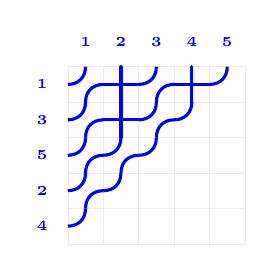
\begin{tikzpicture}[scale=0.45, baseline=(current bounding box.center)]
  \draw[lightgray, very thin, opacity=0.3] (5.3,0) -- (0.3,0);
  \draw[lightgray, very thin, opacity=0.3] (5.3,0) -- (5.3,5);
  \draw[lightgray, very thin, opacity=0.3] (5.3,1) -- (0.3,1);
  \draw[lightgray, very thin, opacity=0.3] (4.3,0) -- (4.3,5);
  \draw[lightgray, very thin, opacity=0.3] (5.3,2) -- (0.3,2);
  \draw[lightgray, very thin, opacity=0.3] (3.3,0) -- (3.3,5);
  \draw[lightgray, very thin, opacity=0.3] (5.3,3) -- (0.3,3);
  \draw[lightgray, very thin, opacity=0.3] (2.3,0) -- (2.3,5);
  \draw[lightgray, very thin, opacity=0.3] (5.3,4) -- (0.3,4);
  \draw[lightgray, very thin, opacity=0.3] (1.3,0) -- (1.3,5);
  \draw[lightgray, very thin, opacity=0.3] (5.3,5) -- (0.3,5);
  \draw[lightgray, very thin, opacity=0.3] (0.3,0) -- (0.3,5);
  \draw[blue, line width=1.125pt] (0.3,4.5) .. controls (0.6,4.5) and (0.8,4.7) .. (0.8,5);
  \draw[blue, line width=1.125pt] (0.8,4) .. controls (0.8,4.3) and (1,4.5) .. (1.3,4.5);
  \draw[blue, line width=1.125pt, line cap=round] (1.3,4.5) -- (2.3,4.5);
  \draw[blue, line width=1.125pt, line cap=round] (1.8,4) -- (1.8,5);
  \draw[blue, line width=1.125pt] (2.3,4.5) .. controls (2.6,4.5) and (2.8,4.7) .. (2.8,5);
  \draw[blue, line width=1.125pt] (2.8,4) .. controls (2.8,4.3) and (3,4.5) .. (3.3,4.5);
  \draw[blue, line width=1.125pt, line cap=round] (3.3,4.5) -- (4.3,4.5);
  \draw[blue, line width=1.125pt, line cap=round] (3.8,4) -- (3.8,5);
  \draw[blue, line width=1.125pt] (4.3,4.5) .. controls (4.6,4.5) and (4.8,4.7) .. (4.8,5);
  \draw[blue, line width=1.125pt] (0.3,3.5) .. controls (0.6,3.5) and (0.8,3.7) .. (0.8,4);
  \draw[blue, line width=1.125pt] (0.8,3) .. controls (0.8,3.3) and (1,3.5) .. (1.3,3.5);
  \draw[blue, line width=1.125pt, line cap=round] (1.3,3.5) -- (2.3,3.5);
  \draw[blue, line width=1.125pt, line cap=round] (1.8,3) -- (1.8,4);
  \draw[blue, line width=1.125pt] (2.3,3.5) .. controls (2.6,3.5) and (2.8,3.7) .. (2.8,4);
  \draw[blue, line width=1.125pt] (2.8,3) .. controls (2.8,3.3) and (3,3.5) .. (3.3,3.5);
  \draw[blue, line width=1.125pt] (3.3,3.5) .. controls (3.6,3.5) and (3.8,3.7) .. (3.8,4);
  \draw[blue, line width=1.125pt] (0.3,2.5) .. controls (0.6,2.5) and (0.8,2.7) .. (0.8,3);
  \draw[blue, line width=1.125pt] (0.8,2) .. controls (0.8,2.3) and (1,2.5) .. (1.3,2.5);
  \draw[blue, line width=1.125pt] (1.3,2.5) .. controls (1.6,2.5) and (1.8,2.7) .. (1.8,3);
  \draw[blue, line width=1.125pt] (1.8,2) .. controls (1.8,2.3) and (2,2.5) .. (2.3,2.5);
  \draw[blue, line width=1.125pt] (2.3,2.5) .. controls (2.6,2.5) and (2.8,2.7) .. (2.8,3);
  \draw[blue, line width=1.125pt] (0.3,1.5) .. controls (0.6,1.5) and (0.8,1.7) .. (0.8,2);
  \draw[blue, line width=1.125pt] (0.8,1) .. controls (0.8,1.3) and (1,1.5) .. (1.3,1.5);
  \draw[blue, line width=1.125pt] (1.3,1.5) .. controls (1.6,1.5) and (1.8,1.7) .. (1.8,2);
  \draw[blue, line width=1.125pt] (0.3,0.5) .. controls (0.6,0.5) and (0.8,0.7) .. (0.8,1);
  \node[font=\tiny\bfseries, text=blue, anchor=south] at (0.8,5.3) {1};
  \node[font=\tiny\bfseries, text=blue, anchor=south] at (1.8,5.3) {2};
  \node[font=\tiny\bfseries, text=blue, anchor=south] at (2.8,5.3) {3};
  \node[font=\tiny\bfseries, text=blue, anchor=south] at (3.8,5.3) {4};
  \node[font=\tiny\bfseries, text=blue, anchor=south] at (4.8,5.3) {5};
  \node[font=\tiny\bfseries, text=blue, anchor=east] at (0,4.5) {1};
  \node[font=\tiny\bfseries, text=blue, anchor=east] at (0,3.5) {3};
  \node[font=\tiny\bfseries, text=blue, anchor=east] at (0,2.5) {5};
  \node[font=\tiny\bfseries, text=blue, anchor=east] at (0,1.5) {2};
  \node[font=\tiny\bfseries, text=blue, anchor=east] at (0,0.5) {4};
\end{tikzpicture}
$$
Applying $\trm^3$ (keeping the bottom $4$ rows) gives the same $4$-row graph with highest weight $b=(0,1,0,2)$:
$$\trm^3(R_1)=\trm^3(R_2)=
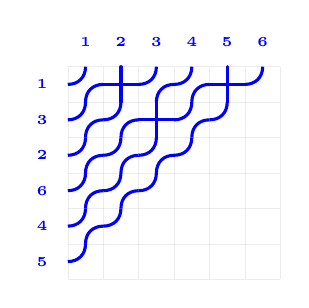
\begin{tikzpicture}[scale=0.45, baseline=(current bounding box.center)]
  \draw[lightgray, very thin, opacity=0.3] (6.3,0) -- (0.3,0);
  \draw[lightgray, very thin, opacity=0.3] (6.3,0) -- (6.3,6);
  \draw[lightgray, very thin, opacity=0.3] (6.3,1) -- (0.3,1);
  \draw[lightgray, very thin, opacity=0.3] (5.3,0) -- (5.3,6);
  \draw[lightgray, very thin, opacity=0.3] (6.3,2) -- (0.3,2);
  \draw[lightgray, very thin, opacity=0.3] (4.3,0) -- (4.3,6);
  \draw[lightgray, very thin, opacity=0.3] (6.3,3) -- (0.3,3);
  \draw[lightgray, very thin, opacity=0.3] (3.3,0) -- (3.3,6);
  \draw[lightgray, very thin, opacity=0.3] (6.3,4) -- (0.3,4);
  \draw[lightgray, very thin, opacity=0.3] (2.3,0) -- (2.3,6);
  \draw[lightgray, very thin, opacity=0.3] (6.3,5) -- (0.3,5);
  \draw[lightgray, very thin, opacity=0.3] (1.3,0) -- (1.3,6);
  \draw[lightgray, very thin, opacity=0.3] (6.3,6) -- (0.3,6);
  \draw[lightgray, very thin, opacity=0.3] (0.3,0) -- (0.3,6);
  \draw[blue, line width=1.125pt] (0.3,5.5) .. controls (0.6,5.5) and (0.8,5.7) .. (0.8,6);
  \draw[blue, line width=1.125pt] (0.8,5) .. controls (0.8,5.3) and (1,5.5) .. (1.3,5.5);
  \draw[blue, line width=1.125pt, line cap=round] (1.3,5.5) -- (2.3,5.5);
  \draw[blue, line width=1.125pt, line cap=round] (1.8,5) -- (1.8,6);
  \draw[blue, line width=1.125pt] (2.3,5.5) .. controls (2.6,5.5) and (2.8,5.7) .. (2.8,6);
  \draw[blue, line width=1.125pt] (2.8,5) .. controls (2.8,5.3) and (3,5.5) .. (3.3,5.5);
  \draw[blue, line width=1.125pt] (3.3,5.5) .. controls (3.6,5.5) and (3.8,5.7) .. (3.8,6);
  \draw[blue, line width=1.125pt] (3.8,5) .. controls (3.8,5.3) and (4,5.5) .. (4.3,5.5);
  \draw[blue, line width=1.125pt, line cap=round] (4.3,5.5) -- (5.3,5.5);
  \draw[blue, line width=1.125pt, line cap=round] (4.8,5) -- (4.8,6);
  \draw[blue, line width=1.125pt] (5.3,5.5) .. controls (5.6,5.5) and (5.8,5.7) .. (5.8,6);
  \draw[blue, line width=1.125pt] (0.3,4.5) .. controls (0.6,4.5) and (0.8,4.7) .. (0.8,5);
  \draw[blue, line width=1.125pt] (0.8,4) .. controls (0.8,4.3) and (1,4.5) .. (1.3,4.5);
  \draw[blue, line width=1.125pt] (1.3,4.5) .. controls (1.6,4.5) and (1.8,4.7) .. (1.8,5);
  \draw[blue, line width=1.125pt] (1.8,4) .. controls (1.8,4.3) and (2,4.5) .. (2.3,4.5);
  \draw[blue, line width=1.125pt, line cap=round] (2.3,4.5) -- (3.3,4.5);
  \draw[blue, line width=1.125pt, line cap=round] (2.8,4) -- (2.8,5);
  \draw[blue, line width=1.125pt] (3.3,4.5) .. controls (3.6,4.5) and (3.8,4.7) .. (3.8,5);
  \draw[blue, line width=1.125pt] (3.8,4) .. controls (3.8,4.3) and (4,4.5) .. (4.3,4.5);
  \draw[blue, line width=1.125pt] (4.3,4.5) .. controls (4.6,4.5) and (4.8,4.7) .. (4.8,5);
  \draw[blue, line width=1.125pt] (0.3,3.5) .. controls (0.6,3.5) and (0.8,3.7) .. (0.8,4);
  \draw[blue, line width=1.125pt] (0.8,3) .. controls (0.8,3.3) and (1,3.5) .. (1.3,3.5);
  \draw[blue, line width=1.125pt] (1.3,3.5) .. controls (1.6,3.5) and (1.8,3.7) .. (1.8,4);
  \draw[blue, line width=1.125pt] (1.8,3) .. controls (1.8,3.3) and (2,3.5) .. (2.3,3.5);
  \draw[blue, line width=1.125pt] (2.3,3.5) .. controls (2.6,3.5) and (2.8,3.7) .. (2.8,4);
  \draw[blue, line width=1.125pt] (2.8,3) .. controls (2.8,3.3) and (3,3.5) .. (3.3,3.5);
  \draw[blue, line width=1.125pt] (3.3,3.5) .. controls (3.6,3.5) and (3.8,3.7) .. (3.8,4);
  \draw[blue, line width=1.125pt] (0.3,2.5) .. controls (0.6,2.5) and (0.8,2.7) .. (0.8,3);
  \draw[blue, line width=1.125pt] (0.8,2) .. controls (0.8,2.3) and (1,2.5) .. (1.3,2.5);
  \draw[blue, line width=1.125pt] (1.3,2.5) .. controls (1.6,2.5) and (1.8,2.7) .. (1.8,3);
  \draw[blue, line width=1.125pt] (1.8,2) .. controls (1.8,2.3) and (2,2.5) .. (2.3,2.5);
  \draw[blue, line width=1.125pt] (2.3,2.5) .. controls (2.6,2.5) and (2.8,2.7) .. (2.8,3);
  \draw[blue, line width=1.125pt] (0.3,1.5) .. controls (0.6,1.5) and (0.8,1.7) .. (0.8,2);
  \draw[blue, line width=1.125pt] (0.8,1) .. controls (0.8,1.3) and (1,1.5) .. (1.3,1.5);
  \draw[blue, line width=1.125pt] (1.3,1.5) .. controls (1.6,1.5) and (1.8,1.7) .. (1.8,2);
  \draw[blue, line width=1.125pt] (0.3,0.5) .. controls (0.6,0.5) and (0.8,0.7) .. (0.8,1);
  \node[font=\tiny\bfseries, text=blue, anchor=south] at (0.8,6.3) {1};
  \node[font=\tiny\bfseries, text=blue, anchor=south] at (1.8,6.3) {2};
  \node[font=\tiny\bfseries, text=blue, anchor=south] at (2.8,6.3) {3};
  \node[font=\tiny\bfseries, text=blue, anchor=south] at (3.8,6.3) {4};
  \node[font=\tiny\bfseries, text=blue, anchor=south] at (4.8,6.3) {5};
  \node[font=\tiny\bfseries, text=blue, anchor=south] at (5.8,6.3) {6};
  \node[font=\tiny\bfseries, text=blue, anchor=east] at (0,5.5) {1};
  \node[font=\tiny\bfseries, text=blue, anchor=east] at (0,4.5) {3};
  \node[font=\tiny\bfseries, text=blue, anchor=east] at (0,3.5) {2};
  \node[font=\tiny\bfseries, text=blue, anchor=east] at (0,2.5) {6};
  \node[font=\tiny\bfseries, text=blue, anchor=east] at (0,1.5) {4};
  \node[font=\tiny\bfseries, text=blue, anchor=east] at (0,0.5) {5};
\end{tikzpicture}
$$

Since there are exactly $2$ such RC graphs, Theorem~\ref{theorem:LRkey} gives $k_{a,b}^c = 2$.
\end{example}



\section{The ring of forest classes of RC graphs}\label{section:forest}

\subsection{Indexed forests, forest invariant}

\begin{definition}[Indexed forests and codes]
  An \emph{indexed forest} $F$ is a pair $(S, T_\bullet)$ where $S$ is a set of positive integers, called the \emph{support} of $F$, and if we write
  $$S=I_1\cup I_2\cup \cdots \cup I_k$$
  where $I_1,I_2,\ldots, I_k$ are the maximal intervals contained in $S$, then $T_\bullet$ is a sequence of binary trees $T_1,T_2,\ldots, T_k$ such that $T_j$ has $|I_j|$ internal nodes for each $j$. The internal nodes of $F$ are denoted by $\mathrm{IN}(F)$. For $v\in \mathrm{IN}(F)$, we denote by $\mathrm{left}(v)$ and $\mathrm{right}(v)$ the left and right children of $v$ respectively, which may not be in $\mathrm{IN}(F)$ if they are leaves, or may be empty.
  
  There is a natural labeling $\lambda_F:\mathrm{IN}(F)\to S$ sending each internal node, say $v\in T_j$, to the unique element of $I_j$ that is at the same index as $v\in T_j$ in the inorder traversal of $T_j$.
  
  The function $\rho_F:\mathrm{IN}(F)\to S$ is defined for an internal node $v\in T_j$ by 
  $$\rho_F(v) = \begin{cases}
  \lambda_F(v)&\mbox{ if }\mathrm{left}(v)\notin\mathrm{IN}(F)\\
  \lambda_F(\mathrm{left}(v))&\mbox{ if }\mathrm{left}(v)\in\mathrm{IN}(F).
  \end{cases}$$
  For each indexed forest $F$, we assign a weak composition $\code(F)$ by
  $$\code_j(F)=\#\{v\in \mathrm{IN}(F): \rho_F(v)=j\}$$
  Then the \emph{forest polynomial} $\forest_F(x)$ is defined by
  $$\forest_F(x) = \sum_{\tau}\prod_{v\in\mathrm{IN}(F)}x_{\tau(v)}$$
  where the sum is over all functions $\tau:\mathrm{IN}(F)\to \mathbb{Z}_{>0}$ such that $\tau(v)\leq \rho_F(v)$ for all $v\in \mathrm{IN}(F)$, $\tau(v)\leq\tau(\mathrm{left}(v))$ for all $v\in \mathrm{IN}(F)$ such that $\mathrm{left}(v)\in \mathrm{IN}(F)$, and $\tau(v)<\tau(\mathrm{right}(v))$ for all $v\in \mathrm{IN}(F)$ such that $\mathrm{right}(v)\in \mathrm{IN}(F)$.

  It is easiest for our purposes to index forest polynomials by weak compositions rather than indexed forests, so we define $\forest_a(x) = \forest_F(x)$ where $F$ is the unique indexed forest such that $\code(F) = a$.
\end{definition}

\begin{definition}[Injective words, forest invariant]
In \cite{nadeau2024ppartitions}, an alphabet $\overline{\mathbb{Z}}$ is defined as the set of pairs of integers $(i,j)$ in lexicographical order, written with the notation $i^{[j]}$. They define $\mathrm{val}(i^{[j]})=i$. An \emph{injective word} is a word $w=w_1w_2\cdots w_k$ such that $w_i\neq w_j$ for all $i\neq j$. An \emph{LBS (local binary search)  labeling} of an indexed forest $F$ is an injective function $\rho:\mathrm{IN}(F)\to \overline{\mathbb{Z}}$ such that
\begin{enumerate}
\item $\rho(\mathrm{left}(v))<\rho(v)$ for all $v\in \mathrm{IN}(F)$ such that $\mathrm{left}(v)\in \mathrm{IN}(F)$.
\item $\rho(v)<\rho(\mathrm{right}(v))$ for all $v\in \mathrm{IN}(F)$ such that $\mathrm{right}(v)\in \mathrm{IN}(F)$.
\item For all $v\in\mathrm{IN}(F)$, $\mathrm{val}(\rho(v)) = \lambda_F(u)$ for some $u\in\mathrm{IN}(F)$.
\end{enumerate}

Following \cite{nadeau2024forest}, given any injective word $w = w_1\cdots w_m$ in $\overline{\mathbb{Z}}$, we associate to it inductively an indexed forest $F(w)$, an LBS labeling $P(w)$ of $F(w)$, and an injective ``time-stamp'' labeling $Q(w):\mathrm{IN}(F(w))\to\{1,\ldots,m\}$ as follows. If $m=0$, then $F(w)$ is the empty forest. Otherwise write $w = w'a$ with $w' = w_1\cdots w_{m-1}$, and assume $F' := F(w')$, $P' := P(w')$, and $Q' := Q(w')$ have already been constructed; let $S'$ be the support of $F'$, and let $S' = I_1\cup\cdots\cup I_k$ be its decomposition into maximal intervals (listed left to right). For each $j$, denote by $u_j$ the root of the tree of $F'$ supported on $I_j$, and set $a_j := P'(u_j)$. We obtain $F(w)$ by adjoining a new internal node $u$ to $F'$, with attachments determined by $i := \mathrm{val}(a)$:
\begin{itemize}
\item If $i\notin S'$, then $u$ is the root of a new tree, with left child $u_j$ when $i-1\in I_j$ (otherwise no left child), and right child $u_j$ when $i+1\in I_j$ (otherwise no right child).
\item If $i\in I_j$, then we compare $a$ with $a_j$ in the order on $\overline{\mathbb{Z}}$:
\begin{itemize}
\item if $a>a_j$, then $u_j$ becomes the left child of $u$; additionally, if $\max(I_j)+2\in S'$ (necessarily $\max(I_j)+2 = \min(I_{j+1})$), then $u_{j+1}$ becomes the right child of $u$;
\item if $a<a_j$, then $u_j$ becomes the right child of $u$; additionally, if $\min(I_j)-2\in S'$ (necessarily $\min(I_j)-2=\max(I_{j-1})$), then $u_{j-1}$ becomes the left child of $u$.
\end{itemize}
\end{itemize}
The remaining roots of $F'$ become roots of $F(w)$ unchanged. We then extend $P'$ to $P(w)$ by setting $P(w)(u) := a$, and extend $Q'$ to $Q(w)$ by setting $Q(w)(u) := m$. The pair $(P(w), Q(w))$ is the \emph{$\Omega$-insertion} of $w$.
\end{definition}

The importance of this algorithm is

\begin{theorem}[{\cite[Theorem~5.1]{nadeau2024forest}}]
The correspondence $w\mapsto (P(w), Q(w))$ is a bijection between the following two sets:
\begin{enumerate}
\item Injective words $w$ with letters in $\overline{\mathbb{Z}}$, and
\item Pairs $(P, Q)$ such that $P \in \mathrm{LBS}(F)$ and $Q \in \mathrm{Dec}(F)$ for a common indexed forest $F$.
\end{enumerate}
\end{theorem}


\begin{definition}[Injectification, $\equiv_\forest$]
  For a word $\mathbf{r}$ in the alphabet $\mathbb{Z}$, we may canonically turn $\mathbf{r}$ into an injective word in the alphabet $\overline{\mathbb{Z}}$ by assigning superscripts consecutively starting at $1$ to break ties between equal letters.

Let $\mathbf{r}_1$ and $\mathbf{r}_2$ be reduced words. Then we say that $\mathbf{r}_1\equiv_\forest\mathbf{r}_2$ if $P(\overline{\mathbf{r}_1}) = P(\overline{\mathbf{r}_2})$. Naturally, we may apply this to RC graphs as well: for RC graphs $R_1$ and $R_2$, we say that $R_1\equiv_\forest R_2$ if $\overline{\mathrm{word}(R_1)}\equiv_\forest \overline{\mathrm{word}(R_2)}$. For a permutation $w$, we denote by $\mathcal{C}_\forest(w)$ the set of equivalence classes of reduced words for $w$ under $\equiv_\forest$.
\end{definition}

\begin{theorem}[{\cite[Theorem~1.4]{nadeau2024forest}}] \label{theorem:forestforest}
  Let $w\in S_\infty$. Then we have

  $$\sch_w(x) = \sum_{C\in \mathcal{C}_\forest(w)} \forest_{\code_\forest(C)}(x)$$
\end{theorem}


\subsection{The dual forest basis and the ring of forest classes of RC graphs}

\begin{definition}[The dual forest basis]
  For a weak composition $a$ of length $n$, define $\forest_a^*\in \dcoma_n$ to be the unique element such that $\langle \forest_a^*, \forest_b\rangle = \delta_{a,b}$ for all weak compositions $b$.
\end{definition}

\begin{theorem}\label{theorem:forestformula}
  We have the following.
  \begin{itemize}
\item[I] Let $R\in \BRC$ be a bounded RC graph. Then the forest polynomial $\forest_{\fcode(R)}$ is equal to
$$\forest_{\fcode(R)}(x)=\sum_{R'\equiv_{\forest} R} x^{\wtt(R')}$$

\item[II] Let $c$ be a weak composition. Then dual forest polynomial $\forest^*_c$ is equal to
$$\forest^*_c = \sum_{[R]\in\mathcal{C}_\forest(c)} \dsch_{\wof{R}}^{\hr(R)}$$
  \end{itemize}
\end{theorem}


\begin{proof}[Proof of Theorem \ref{theorem:forestformula}]
  Part I of this theorem follows from the fact that for any equivalence class of words $W$ that have the same $P$-LBS, $\forest_{\code_\forest(W)}(x)$ is the sum of the compatible sequences on the words in $W$, which are simply the RC graphs in the corresponding equivalence class of RC graphs. Part II follows from Theorem \ref{theorem:forestforest} and the definition of the dual Schubert basis.
\end{proof}

Guo and Woodruff \cite{guo2026forest} also published an alternative RC graph formula for forest polynomials.


\begin{proposition}
Let $c$ be a weak composition of length $p$. Let $\RC_\forest(c)$ be the set of RC graphs with $\wtt(R) = c$ such that $\mathrm{word}(\mathbb{Y}_\forest(R))$ is minimal in lexicographical order among all RC graphs $R'$ such that $\code_\forest(R)=\code_\forest(R')$.
$$[c] = \sum_{R\in\RC_\forest(c)} \forest_{\code_\forest(R)}^*$$
\end{proposition}

\begin{definition}[The submodule $\Gamma\subseteq \BRC$]
  Let $\Gamma$ be the $\mathbb{Z}$-submodule of $\BRC$ generated by the elements $R_1-R_2$ such that $R_1\equiv_\forest R_2$.

\end{definition}

\begin{lemma} \label{lemma:forestideal}
  $\Gamma$ is a two-sided ideal of $\BRC$.
\end{lemma}
\begin{proof}
  The fact that $\Gamma$ is a left ideal follows from the fact that the products $R\sqcupplus R_1$ and $R\sqcupplus R_2$ have the same first $\hr(R)$ rows, and the rows below are simply shifts of $R_1$ and $R_2$. In terms of the resulting words, the shifted $\mathrm{word}(R_1)$ and $\mathrm{word}(R_2)$ are suffixes of $\mathrm{word}(R\sqcupplus R_1)$ and $\mathrm{word}(R\sqcupplus R_2)$. The $\equiv_\forest$ equivalence is determined by local swaps of pairs of letters that are related in a shift-invariant \cite[Proposition~5.8]{nadeau2024forest} and prefix-invariant \cite[Lemma~5.9]{nadeau2024forest} way, from which the result follows, since the prefixes are identical and the suffixes are related in the same way as $\mathrm{word}(R_1)$ and $\mathrm{word}(R_2)$.

  To prove that $\Gamma$ is a right ideal, assume $\mathrm{word}(R_1)$ and $\mathrm{word}(R_2)$ differ by a single local swap of adjacent letters $a$ and $b$ in the same equivalence class, with $a$ to the left of $b$ in $\mathrm{word}(R_1)$ and to the right of $b$ in $\mathrm{word}(R_2)$. It suffices to consider only the case where $R$ is empty to show that
  $$R_1\sqcupplus R - R_2\sqcupplus R\in \Gamma$$
  for any $R$. According to \cite{nadeau2024forest}, the local swap of $a$ and $b$ is a commutation move, and we may reduce to the case where $a$ and $b$ are the last two letters of $\mathrm{word}(R_1)$, and that $b$ is the last descent of $\wof{R_1}$. For any empty $R$, the position $a$ will remain the same. For any term not identical to $R_1$, the suffix of the word will be $ab'$ where $b'>b$. For each $b'$, there will be precisely one matching term with suffix $b'a$ and identical prefix. The local swap of $a$ and $b'$ in the suffix is a valid local swap, so the resulting terms are all in $\Gamma$, and we are done.
\end{proof}

\begin{lemma}
  The homomorphism $\alpha:\BRC\to\dcoma$ factors through the quotient $\BRC/\Gamma$.
\end{lemma}
\begin{proof}
This is because the generators of $\Gamma$ are all in $\Omega$.
\end{proof}

\begin{definition}
For a composition $a$, define  an element $F_a\in\BRC/\Gamma$ by
$$F_a =\sum_{[R]\in\mathcal{C}_\forest(a)} [R]$$
\end{definition}

\begin{proposition}
The elements $F_a\in\BRC/\Gamma$ form an additive basis of a subring isomorphic to $\dcoma$ under the homomorphism $\alpha:\BRC/\Gamma\to \dcoma$, and 
$$\alpha(F_a) = \forest_a^*$$
\end{proposition}
\begin{proof}
As before, the last statement is simply Theorem \ref{theorem:forestformula}. The $F_a$ actually consist of pairwise disjoint sets of RC graphs, the set of all such is clearly independent. To show that they span a subring, consider the homomorphism $\alpha:\BRC/\Gamma\to \dcoma$. We have that $\alpha(F_a)=\forest_a^*$, and since these are linearly independent, it follows that the kernel of $\alpha$ intersects trivially with the span of the $F_a$. Since $\alpha$ is a homomorphism, it follows that $\alpha$ is injective on the span of the $F_a$, and since 
$$\alpha(F_a)\sqcupplus\alpha(F_b) = \forest_a^*\sqcupplus\forest_b^*=\sum_{c}f_{ab}^c\,\forest_c^*=\sum f_{a,b}^c\,\alpha(F_c),$$ 
it follows that $F_a\sqcupplus F_b$ is a linear combination of the $F_c$, so the span of the $F_a$ is closed under multiplication, so that $\alpha$ is an isomorphism and we are done.
\end{proof}

\begin{proof}[Proof of Theorem \ref{theorem:LRforest}]
  The coefficient of $F_c$ in $F_a\sqcupplus F_b$ is the same as the coefficient of $\forest_c^*$ in $\forest_a^*\sqcupplus\forest_b^*$, which is $f_{a,b}^c$ by definition. Since each of the summands of $F_c$ that are equivalence classes of RC graphs are distinct from the summands of any other forest element and each other, we need only consider one of the summands to read off the coefficient. The result follows.
\end{proof}

\begin{example}[Computing $\forest_a^*\sqcupplus\forest_b^*$ for $a=(0,0,2,0,2)$, $b=(0,1,0,0,2)$]\label{example:LRforest}
Let
$$a=(0,0,2,0,2),\qquad b=(0,1,0,0,2),\qquad c=(0,0,1,0,1,0,2,0,0,3).$$
Here $p=q=5$, so by Theorem~\ref{theorem:LRforest} the coefficient $f_{a,b}^c$ counts the $R$ in a fixed forest class $\mathcal{C}_\forest(c)$ of $10$-row RC graphs satisfying
$$\clp^{5}(R)\in\mathcal{C}_\forest(a),\quad \trm^{5}(R)\in\mathcal{C}_\forest(b),\quad \wtt(\clp^{5}(R))=a,\quad \wtt(\trm^{5}(R))=b.$$

Writing an RC graph as the set of ordered pairs $(i,j)\in\mathbb{Z}_{>0}\times\mathbb{Z}_{>0}$ recording the (row,\,column) of each crossing, there are exactly two such $R$, namely
\begin{align*}
R_1 &= \{(3,1),(3,2),(5,3),(5,8),(7,1),(10,1),(10,2)\},\\
R_2 &= \{(3,1),(3,6),(5,1),(5,8),(7,1),(10,1),(10,2)\}.
\end{align*}
Both have permutation
$$\wof{R_1}=\wof{R_2}=(1,2,4,3,6,5,9,7,8,13,10,11,12),$$
and they share a common clip/trim pair
$$\clp^{5}(R_i)=\{(3,1),(3,2),(5,1),(5,2)\},\qquad \trm^{5}(R_i)=\{(2,1),(5,1),(5,2)\},$$
with $\wtt(\clp^{5}(R_i))=a$ and $\wtt(\trm^{5}(R_i))=b$.

\begin{figure}[h]
\centering
\begin{tabular}{cc}
\resizebox{0.43\textwidth}{!}{\input{forest_lr_R1.tikz}} &
\resizebox{0.43\textwidth}{!}{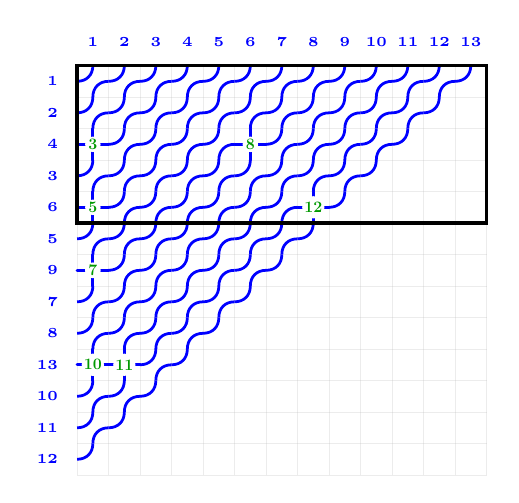
\begin{tikzpicture}[scale=0.4]
  \draw[lightgray, very thin, opacity=0.3] (13,0) -- (0,0);
  \draw[lightgray, very thin, opacity=0.3] (13,0) -- (13,13);
  \draw[lightgray, very thin, opacity=0.3] (13,1) -- (0,1);
  \draw[lightgray, very thin, opacity=0.3] (12,0) -- (12,13);
  \draw[lightgray, very thin, opacity=0.3] (13,2) -- (0,2);
  \draw[lightgray, very thin, opacity=0.3] (11,0) -- (11,13);
  \draw[lightgray, very thin, opacity=0.3] (13,3) -- (0,3);
  \draw[lightgray, very thin, opacity=0.3] (10,0) -- (10,13);
  \draw[lightgray, very thin, opacity=0.3] (13,4) -- (0,4);
  \draw[lightgray, very thin, opacity=0.3] (9,0) -- (9,13);
  \draw[lightgray, very thin, opacity=0.3] (13,5) -- (0,5);
  \draw[lightgray, very thin, opacity=0.3] (8,0) -- (8,13);
  \draw[lightgray, very thin, opacity=0.3] (13,6) -- (0,6);
  \draw[lightgray, very thin, opacity=0.3] (7,0) -- (7,13);
  \draw[lightgray, very thin, opacity=0.3] (13,7) -- (0,7);
  \draw[lightgray, very thin, opacity=0.3] (6,0) -- (6,13);
  \draw[lightgray, very thin, opacity=0.3] (13,8) -- (0,8);
  \draw[lightgray, very thin, opacity=0.3] (5,0) -- (5,13);
  \draw[lightgray, very thin, opacity=0.3] (13,9) -- (0,9);
  \draw[lightgray, very thin, opacity=0.3] (4,0) -- (4,13);
  \draw[lightgray, very thin, opacity=0.3] (13,10) -- (0,10);
  \draw[lightgray, very thin, opacity=0.3] (3,0) -- (3,13);
  \draw[lightgray, very thin, opacity=0.3] (13,11) -- (0,11);
  \draw[lightgray, very thin, opacity=0.3] (2,0) -- (2,13);
  \draw[lightgray, very thin, opacity=0.3] (13,12) -- (0,12);
  \draw[lightgray, very thin, opacity=0.3] (1,0) -- (1,13);
  \draw[lightgray, very thin, opacity=0.3] (13,13) -- (0,13);
  \draw[lightgray, very thin, opacity=0.3] (0,0) -- (0,13);
  \draw[blue, line width=1.0pt] (0,12.5) .. controls (0.3,12.5) and (0.5,12.7) .. (0.5,13);
  \draw[blue, line width=1.0pt] (0.5,12) .. controls (0.5,12.3) and (0.7,12.5) .. (1,12.5);
  \draw[blue, line width=1.0pt] (1,12.5) .. controls (1.3,12.5) and (1.5,12.7) .. (1.5,13);
  \draw[blue, line width=1.0pt] (1.5,12) .. controls (1.5,12.3) and (1.7,12.5) .. (2,12.5);
  \draw[blue, line width=1.0pt] (2,12.5) .. controls (2.3,12.5) and (2.5,12.7) .. (2.5,13);
  \draw[blue, line width=1.0pt] (2.5,12) .. controls (2.5,12.3) and (2.7,12.5) .. (3,12.5);
  \draw[blue, line width=1.0pt] (3,12.5) .. controls (3.3,12.5) and (3.5,12.7) .. (3.5,13);
  \draw[blue, line width=1.0pt] (3.5,12) .. controls (3.5,12.3) and (3.7,12.5) .. (4,12.5);
  \draw[blue, line width=1.0pt] (4,12.5) .. controls (4.3,12.5) and (4.5,12.7) .. (4.5,13);
  \draw[blue, line width=1.0pt] (4.5,12) .. controls (4.5,12.3) and (4.7,12.5) .. (5,12.5);
  \draw[blue, line width=1.0pt] (5,12.5) .. controls (5.3,12.5) and (5.5,12.7) .. (5.5,13);
  \draw[blue, line width=1.0pt] (5.5,12) .. controls (5.5,12.3) and (5.7,12.5) .. (6,12.5);
  \draw[blue, line width=1.0pt] (6,12.5) .. controls (6.3,12.5) and (6.5,12.7) .. (6.5,13);
  \draw[blue, line width=1.0pt] (6.5,12) .. controls (6.5,12.3) and (6.7,12.5) .. (7,12.5);
  \draw[blue, line width=1.0pt] (7,12.5) .. controls (7.3,12.5) and (7.5,12.7) .. (7.5,13);
  \draw[blue, line width=1.0pt] (7.5,12) .. controls (7.5,12.3) and (7.7,12.5) .. (8,12.5);
  \draw[blue, line width=1.0pt] (8,12.5) .. controls (8.3,12.5) and (8.5,12.7) .. (8.5,13);
  \draw[blue, line width=1.0pt] (8.5,12) .. controls (8.5,12.3) and (8.7,12.5) .. (9,12.5);
  \draw[blue, line width=1.0pt] (9,12.5) .. controls (9.3,12.5) and (9.5,12.7) .. (9.5,13);
  \draw[blue, line width=1.0pt] (9.5,12) .. controls (9.5,12.3) and (9.7,12.5) .. (10,12.5);
  \draw[blue, line width=1.0pt] (10,12.5) .. controls (10.3,12.5) and (10.5,12.7) .. (10.5,13);
  \draw[blue, line width=1.0pt] (10.5,12) .. controls (10.5,12.3) and (10.7,12.5) .. (11,12.5);
  \draw[blue, line width=1.0pt] (11,12.5) .. controls (11.3,12.5) and (11.5,12.7) .. (11.5,13);
  \draw[blue, line width=1.0pt] (11.5,12) .. controls (11.5,12.3) and (11.7,12.5) .. (12,12.5);
  \draw[blue, line width=1.0pt] (12,12.5) .. controls (12.3,12.5) and (12.5,12.7) .. (12.5,13);
  \draw[blue, line width=1.0pt] (0,11.5) .. controls (0.3,11.5) and (0.5,11.7) .. (0.5,12);
  \draw[blue, line width=1.0pt] (0.5,11) .. controls (0.5,11.3) and (0.7,11.5) .. (1,11.5);
  \draw[blue, line width=1.0pt] (1,11.5) .. controls (1.3,11.5) and (1.5,11.7) .. (1.5,12);
  \draw[blue, line width=1.0pt] (1.5,11) .. controls (1.5,11.3) and (1.7,11.5) .. (2,11.5);
  \draw[blue, line width=1.0pt] (2,11.5) .. controls (2.3,11.5) and (2.5,11.7) .. (2.5,12);
  \draw[blue, line width=1.0pt] (2.5,11) .. controls (2.5,11.3) and (2.7,11.5) .. (3,11.5);
  \draw[blue, line width=1.0pt] (3,11.5) .. controls (3.3,11.5) and (3.5,11.7) .. (3.5,12);
  \draw[blue, line width=1.0pt] (3.5,11) .. controls (3.5,11.3) and (3.7,11.5) .. (4,11.5);
  \draw[blue, line width=1.0pt] (4,11.5) .. controls (4.3,11.5) and (4.5,11.7) .. (4.5,12);
  \draw[blue, line width=1.0pt] (4.5,11) .. controls (4.5,11.3) and (4.7,11.5) .. (5,11.5);
  \draw[blue, line width=1.0pt] (5,11.5) .. controls (5.3,11.5) and (5.5,11.7) .. (5.5,12);
  \draw[blue, line width=1.0pt] (5.5,11) .. controls (5.5,11.3) and (5.7,11.5) .. (6,11.5);
  \draw[blue, line width=1.0pt] (6,11.5) .. controls (6.3,11.5) and (6.5,11.7) .. (6.5,12);
  \draw[blue, line width=1.0pt] (6.5,11) .. controls (6.5,11.3) and (6.7,11.5) .. (7,11.5);
  \draw[blue, line width=1.0pt] (7,11.5) .. controls (7.3,11.5) and (7.5,11.7) .. (7.5,12);
  \draw[blue, line width=1.0pt] (7.5,11) .. controls (7.5,11.3) and (7.7,11.5) .. (8,11.5);
  \draw[blue, line width=1.0pt] (8,11.5) .. controls (8.3,11.5) and (8.5,11.7) .. (8.5,12);
  \draw[blue, line width=1.0pt] (8.5,11) .. controls (8.5,11.3) and (8.7,11.5) .. (9,11.5);
  \draw[blue, line width=1.0pt] (9,11.5) .. controls (9.3,11.5) and (9.5,11.7) .. (9.5,12);
  \draw[blue, line width=1.0pt] (9.5,11) .. controls (9.5,11.3) and (9.7,11.5) .. (10,11.5);
  \draw[blue, line width=1.0pt] (10,11.5) .. controls (10.3,11.5) and (10.5,11.7) .. (10.5,12);
  \draw[blue, line width=1.0pt] (10.5,11) .. controls (10.5,11.3) and (10.7,11.5) .. (11,11.5);
  \draw[blue, line width=1.0pt] (11,11.5) .. controls (11.3,11.5) and (11.5,11.7) .. (11.5,12);
  \draw[blue, line width=1.0pt, line cap=round] (0,10.5) -- (1,10.5);
  \draw[blue, line width=1.0pt, line cap=round] (0.5,10) -- (0.5,11);
  \draw[blue, line width=1.0pt] (1,10.5) .. controls (1.3,10.5) and (1.5,10.7) .. (1.5,11);
  \draw[blue, line width=1.0pt] (1.5,10) .. controls (1.5,10.3) and (1.7,10.5) .. (2,10.5);
  \draw[blue, line width=1.0pt] (2,10.5) .. controls (2.3,10.5) and (2.5,10.7) .. (2.5,11);
  \draw[blue, line width=1.0pt] (2.5,10) .. controls (2.5,10.3) and (2.7,10.5) .. (3,10.5);
  \draw[blue, line width=1.0pt] (3,10.5) .. controls (3.3,10.5) and (3.5,10.7) .. (3.5,11);
  \draw[blue, line width=1.0pt] (3.5,10) .. controls (3.5,10.3) and (3.7,10.5) .. (4,10.5);
  \draw[blue, line width=1.0pt] (4,10.5) .. controls (4.3,10.5) and (4.5,10.7) .. (4.5,11);
  \draw[blue, line width=1.0pt] (4.5,10) .. controls (4.5,10.3) and (4.7,10.5) .. (5,10.5);
  \draw[blue, line width=1.0pt, line cap=round] (5,10.5) -- (6,10.5);
  \draw[blue, line width=1.0pt, line cap=round] (5.5,10) -- (5.5,11);
  \draw[blue, line width=1.0pt] (6,10.5) .. controls (6.3,10.5) and (6.5,10.7) .. (6.5,11);
  \draw[blue, line width=1.0pt] (6.5,10) .. controls (6.5,10.3) and (6.7,10.5) .. (7,10.5);
  \draw[blue, line width=1.0pt] (7,10.5) .. controls (7.3,10.5) and (7.5,10.7) .. (7.5,11);
  \draw[blue, line width=1.0pt] (7.5,10) .. controls (7.5,10.3) and (7.7,10.5) .. (8,10.5);
  \draw[blue, line width=1.0pt] (8,10.5) .. controls (8.3,10.5) and (8.5,10.7) .. (8.5,11);
  \draw[blue, line width=1.0pt] (8.5,10) .. controls (8.5,10.3) and (8.7,10.5) .. (9,10.5);
  \draw[blue, line width=1.0pt] (9,10.5) .. controls (9.3,10.5) and (9.5,10.7) .. (9.5,11);
  \draw[blue, line width=1.0pt] (9.5,10) .. controls (9.5,10.3) and (9.7,10.5) .. (10,10.5);
  \draw[blue, line width=1.0pt] (10,10.5) .. controls (10.3,10.5) and (10.5,10.7) .. (10.5,11);
  \draw[blue, line width=1.0pt] (0,9.5) .. controls (0.3,9.5) and (0.5,9.7) .. (0.5,10);
  \draw[blue, line width=1.0pt] (0.5,9) .. controls (0.5,9.3) and (0.7,9.5) .. (1,9.5);
  \draw[blue, line width=1.0pt] (1,9.5) .. controls (1.3,9.5) and (1.5,9.7) .. (1.5,10);
  \draw[blue, line width=1.0pt] (1.5,9) .. controls (1.5,9.3) and (1.7,9.5) .. (2,9.5);
  \draw[blue, line width=1.0pt] (2,9.5) .. controls (2.3,9.5) and (2.5,9.7) .. (2.5,10);
  \draw[blue, line width=1.0pt] (2.5,9) .. controls (2.5,9.3) and (2.7,9.5) .. (3,9.5);
  \draw[blue, line width=1.0pt] (3,9.5) .. controls (3.3,9.5) and (3.5,9.7) .. (3.5,10);
  \draw[blue, line width=1.0pt] (3.5,9) .. controls (3.5,9.3) and (3.7,9.5) .. (4,9.5);
  \draw[blue, line width=1.0pt] (4,9.5) .. controls (4.3,9.5) and (4.5,9.7) .. (4.5,10);
  \draw[blue, line width=1.0pt] (4.5,9) .. controls (4.5,9.3) and (4.7,9.5) .. (5,9.5);
  \draw[blue, line width=1.0pt] (5,9.5) .. controls (5.3,9.5) and (5.5,9.7) .. (5.5,10);
  \draw[blue, line width=1.0pt] (5.5,9) .. controls (5.5,9.3) and (5.7,9.5) .. (6,9.5);
  \draw[blue, line width=1.0pt] (6,9.5) .. controls (6.3,9.5) and (6.5,9.7) .. (6.5,10);
  \draw[blue, line width=1.0pt] (6.5,9) .. controls (6.5,9.3) and (6.7,9.5) .. (7,9.5);
  \draw[blue, line width=1.0pt] (7,9.5) .. controls (7.3,9.5) and (7.5,9.7) .. (7.5,10);
  \draw[blue, line width=1.0pt] (7.5,9) .. controls (7.5,9.3) and (7.7,9.5) .. (8,9.5);
  \draw[blue, line width=1.0pt] (8,9.5) .. controls (8.3,9.5) and (8.5,9.7) .. (8.5,10);
  \draw[blue, line width=1.0pt] (8.5,9) .. controls (8.5,9.3) and (8.7,9.5) .. (9,9.5);
  \draw[blue, line width=1.0pt] (9,9.5) .. controls (9.3,9.5) and (9.5,9.7) .. (9.5,10);
  \draw[blue, line width=1.0pt, line cap=round] (0,8.5) -- (1,8.5);
  \draw[blue, line width=1.0pt, line cap=round] (0.5,8) -- (0.5,9);
  \draw[blue, line width=1.0pt] (1,8.5) .. controls (1.3,8.5) and (1.5,8.7) .. (1.5,9);
  \draw[blue, line width=1.0pt] (1.5,8) .. controls (1.5,8.3) and (1.7,8.5) .. (2,8.5);
  \draw[blue, line width=1.0pt] (2,8.5) .. controls (2.3,8.5) and (2.5,8.7) .. (2.5,9);
  \draw[blue, line width=1.0pt] (2.5,8) .. controls (2.5,8.3) and (2.7,8.5) .. (3,8.5);
  \draw[blue, line width=1.0pt] (3,8.5) .. controls (3.3,8.5) and (3.5,8.7) .. (3.5,9);
  \draw[blue, line width=1.0pt] (3.5,8) .. controls (3.5,8.3) and (3.7,8.5) .. (4,8.5);
  \draw[blue, line width=1.0pt] (4,8.5) .. controls (4.3,8.5) and (4.5,8.7) .. (4.5,9);
  \draw[blue, line width=1.0pt] (4.5,8) .. controls (4.5,8.3) and (4.7,8.5) .. (5,8.5);
  \draw[blue, line width=1.0pt] (5,8.5) .. controls (5.3,8.5) and (5.5,8.7) .. (5.5,9);
  \draw[blue, line width=1.0pt] (5.5,8) .. controls (5.5,8.3) and (5.7,8.5) .. (6,8.5);
  \draw[blue, line width=1.0pt] (6,8.5) .. controls (6.3,8.5) and (6.5,8.7) .. (6.5,9);
  \draw[blue, line width=1.0pt] (6.5,8) .. controls (6.5,8.3) and (6.7,8.5) .. (7,8.5);
  \draw[blue, line width=1.0pt, line cap=round] (7,8.5) -- (8,8.5);
  \draw[blue, line width=1.0pt, line cap=round] (7.5,8) -- (7.5,9);
  \draw[blue, line width=1.0pt] (8,8.5) .. controls (8.3,8.5) and (8.5,8.7) .. (8.5,9);
  \draw[blue, line width=1.0pt] (0,7.5) .. controls (0.3,7.5) and (0.5,7.7) .. (0.5,8);
  \draw[blue, line width=1.0pt] (0.5,7) .. controls (0.5,7.3) and (0.7,7.5) .. (1,7.5);
  \draw[blue, line width=1.0pt] (1,7.5) .. controls (1.3,7.5) and (1.5,7.7) .. (1.5,8);
  \draw[blue, line width=1.0pt] (1.5,7) .. controls (1.5,7.3) and (1.7,7.5) .. (2,7.5);
  \draw[blue, line width=1.0pt] (2,7.5) .. controls (2.3,7.5) and (2.5,7.7) .. (2.5,8);
  \draw[blue, line width=1.0pt] (2.5,7) .. controls (2.5,7.3) and (2.7,7.5) .. (3,7.5);
  \draw[blue, line width=1.0pt] (3,7.5) .. controls (3.3,7.5) and (3.5,7.7) .. (3.5,8);
  \draw[blue, line width=1.0pt] (3.5,7) .. controls (3.5,7.3) and (3.7,7.5) .. (4,7.5);
  \draw[blue, line width=1.0pt] (4,7.5) .. controls (4.3,7.5) and (4.5,7.7) .. (4.5,8);
  \draw[blue, line width=1.0pt] (4.5,7) .. controls (4.5,7.3) and (4.7,7.5) .. (5,7.5);
  \draw[blue, line width=1.0pt] (5,7.5) .. controls (5.3,7.5) and (5.5,7.7) .. (5.5,8);
  \draw[blue, line width=1.0pt] (5.5,7) .. controls (5.5,7.3) and (5.7,7.5) .. (6,7.5);
  \draw[blue, line width=1.0pt] (6,7.5) .. controls (6.3,7.5) and (6.5,7.7) .. (6.5,8);
  \draw[blue, line width=1.0pt] (6.5,7) .. controls (6.5,7.3) and (6.7,7.5) .. (7,7.5);
  \draw[blue, line width=1.0pt] (7,7.5) .. controls (7.3,7.5) and (7.5,7.7) .. (7.5,8);
  \draw[blue, line width=1.0pt, line cap=round] (0,6.5) -- (1,6.5);
  \draw[blue, line width=1.0pt, line cap=round] (0.5,6) -- (0.5,7);
  \draw[blue, line width=1.0pt] (1,6.5) .. controls (1.3,6.5) and (1.5,6.7) .. (1.5,7);
  \draw[blue, line width=1.0pt] (1.5,6) .. controls (1.5,6.3) and (1.7,6.5) .. (2,6.5);
  \draw[blue, line width=1.0pt] (2,6.5) .. controls (2.3,6.5) and (2.5,6.7) .. (2.5,7);
  \draw[blue, line width=1.0pt] (2.5,6) .. controls (2.5,6.3) and (2.7,6.5) .. (3,6.5);
  \draw[blue, line width=1.0pt] (3,6.5) .. controls (3.3,6.5) and (3.5,6.7) .. (3.5,7);
  \draw[blue, line width=1.0pt] (3.5,6) .. controls (3.5,6.3) and (3.7,6.5) .. (4,6.5);
  \draw[blue, line width=1.0pt] (4,6.5) .. controls (4.3,6.5) and (4.5,6.7) .. (4.5,7);
  \draw[blue, line width=1.0pt] (4.5,6) .. controls (4.5,6.3) and (4.7,6.5) .. (5,6.5);
  \draw[blue, line width=1.0pt] (5,6.5) .. controls (5.3,6.5) and (5.5,6.7) .. (5.5,7);
  \draw[blue, line width=1.0pt] (5.5,6) .. controls (5.5,6.3) and (5.7,6.5) .. (6,6.5);
  \draw[blue, line width=1.0pt] (6,6.5) .. controls (6.3,6.5) and (6.5,6.7) .. (6.5,7);
  \draw[blue, line width=1.0pt] (0,5.5) .. controls (0.3,5.5) and (0.5,5.7) .. (0.5,6);
  \draw[blue, line width=1.0pt] (0.5,5) .. controls (0.5,5.3) and (0.7,5.5) .. (1,5.5);
  \draw[blue, line width=1.0pt] (1,5.5) .. controls (1.3,5.5) and (1.5,5.7) .. (1.5,6);
  \draw[blue, line width=1.0pt] (1.5,5) .. controls (1.5,5.3) and (1.7,5.5) .. (2,5.5);
  \draw[blue, line width=1.0pt] (2,5.5) .. controls (2.3,5.5) and (2.5,5.7) .. (2.5,6);
  \draw[blue, line width=1.0pt] (2.5,5) .. controls (2.5,5.3) and (2.7,5.5) .. (3,5.5);
  \draw[blue, line width=1.0pt] (3,5.5) .. controls (3.3,5.5) and (3.5,5.7) .. (3.5,6);
  \draw[blue, line width=1.0pt] (3.5,5) .. controls (3.5,5.3) and (3.7,5.5) .. (4,5.5);
  \draw[blue, line width=1.0pt] (4,5.5) .. controls (4.3,5.5) and (4.5,5.7) .. (4.5,6);
  \draw[blue, line width=1.0pt] (4.5,5) .. controls (4.5,5.3) and (4.7,5.5) .. (5,5.5);
  \draw[blue, line width=1.0pt] (5,5.5) .. controls (5.3,5.5) and (5.5,5.7) .. (5.5,6);
  \draw[blue, line width=1.0pt] (0,4.5) .. controls (0.3,4.5) and (0.5,4.7) .. (0.5,5);
  \draw[blue, line width=1.0pt] (0.5,4) .. controls (0.5,4.3) and (0.7,4.5) .. (1,4.5);
  \draw[blue, line width=1.0pt] (1,4.5) .. controls (1.3,4.5) and (1.5,4.7) .. (1.5,5);
  \draw[blue, line width=1.0pt] (1.5,4) .. controls (1.5,4.3) and (1.7,4.5) .. (2,4.5);
  \draw[blue, line width=1.0pt] (2,4.5) .. controls (2.3,4.5) and (2.5,4.7) .. (2.5,5);
  \draw[blue, line width=1.0pt] (2.5,4) .. controls (2.5,4.3) and (2.7,4.5) .. (3,4.5);
  \draw[blue, line width=1.0pt] (3,4.5) .. controls (3.3,4.5) and (3.5,4.7) .. (3.5,5);
  \draw[blue, line width=1.0pt] (3.5,4) .. controls (3.5,4.3) and (3.7,4.5) .. (4,4.5);
  \draw[blue, line width=1.0pt] (4,4.5) .. controls (4.3,4.5) and (4.5,4.7) .. (4.5,5);
  \draw[blue, line width=1.0pt, line cap=round] (0,3.5) -- (1,3.5);
  \draw[blue, line width=1.0pt, line cap=round] (0.5,3) -- (0.5,4);
  \draw[blue, line width=1.0pt, line cap=round] (1,3.5) -- (2,3.5);
  \draw[blue, line width=1.0pt, line cap=round] (1.5,3) -- (1.5,4);
  \draw[blue, line width=1.0pt] (2,3.5) .. controls (2.3,3.5) and (2.5,3.7) .. (2.5,4);
  \draw[blue, line width=1.0pt] (2.5,3) .. controls (2.5,3.3) and (2.7,3.5) .. (3,3.5);
  \draw[blue, line width=1.0pt] (3,3.5) .. controls (3.3,3.5) and (3.5,3.7) .. (3.5,4);
  \draw[blue, line width=1.0pt] (0,2.5) .. controls (0.3,2.5) and (0.5,2.7) .. (0.5,3);
  \draw[blue, line width=1.0pt] (0.5,2) .. controls (0.5,2.3) and (0.7,2.5) .. (1,2.5);
  \draw[blue, line width=1.0pt] (1,2.5) .. controls (1.3,2.5) and (1.5,2.7) .. (1.5,3);
  \draw[blue, line width=1.0pt] (1.5,2) .. controls (1.5,2.3) and (1.7,2.5) .. (2,2.5);
  \draw[blue, line width=1.0pt] (2,2.5) .. controls (2.3,2.5) and (2.5,2.7) .. (2.5,3);
  \draw[blue, line width=1.0pt] (0,1.5) .. controls (0.3,1.5) and (0.5,1.7) .. (0.5,2);
  \draw[blue, line width=1.0pt] (0.5,1) .. controls (0.5,1.3) and (0.7,1.5) .. (1,1.5);
  \draw[blue, line width=1.0pt] (1,1.5) .. controls (1.3,1.5) and (1.5,1.7) .. (1.5,2);
  \draw[blue, line width=1.0pt] (0,0.5) .. controls (0.3,0.5) and (0.5,0.7) .. (0.5,1);
  \node[font=\tiny\bfseries, text=blue, anchor=south] at (0.5,13.3) {1};
  \node[font=\tiny\bfseries, text=blue, anchor=south] at (1.5,13.3) {2};
  \node[font=\tiny\bfseries, text=blue, anchor=south] at (2.5,13.3) {3};
  \node[font=\tiny\bfseries, text=blue, anchor=south] at (3.5,13.3) {4};
  \node[font=\tiny\bfseries, text=blue, anchor=south] at (4.5,13.3) {5};
  \node[font=\tiny\bfseries, text=blue, anchor=south] at (5.5,13.3) {6};
  \node[font=\tiny\bfseries, text=blue, anchor=south] at (6.5,13.3) {7};
  \node[font=\tiny\bfseries, text=blue, anchor=south] at (7.5,13.3) {8};
  \node[font=\tiny\bfseries, text=blue, anchor=south] at (8.5,13.3) {9};
  \node[font=\tiny\bfseries, text=blue, anchor=south] at (9.5,13.3) {10};
  \node[font=\tiny\bfseries, text=blue, anchor=south] at (10.5,13.3) {11};
  \node[font=\tiny\bfseries, text=blue, anchor=south] at (11.5,13.3) {12};
  \node[font=\tiny\bfseries, text=blue, anchor=south] at (12.5,13.3) {13};
  \node[font=\tiny\bfseries, text=blue, anchor=east] at (-0.3,12.5) {1};
  \node[font=\tiny\bfseries, text=blue, anchor=east] at (-0.3,11.5) {2};
  \node[font=\tiny\bfseries, text=blue, anchor=east] at (-0.3,10.5) {4};
  \node[font=\tiny\bfseries, text=blue, anchor=east] at (-0.3,9.5) {3};
  \node[font=\tiny\bfseries, text=blue, anchor=east] at (-0.3,8.5) {6};
  \node[font=\tiny\bfseries, text=blue, anchor=east] at (-0.3,7.5) {5};
  \node[font=\tiny\bfseries, text=blue, anchor=east] at (-0.3,6.5) {9};
  \node[font=\tiny\bfseries, text=blue, anchor=east] at (-0.3,5.5) {7};
  \node[font=\tiny\bfseries, text=blue, anchor=east] at (-0.3,4.5) {8};
  \node[font=\tiny\bfseries, text=blue, anchor=east] at (-0.3,3.5) {13};
  \node[font=\tiny\bfseries, text=blue, anchor=east] at (-0.3,2.5) {10};
  \node[font=\tiny\bfseries, text=blue, anchor=east] at (-0.3,1.5) {11};
  \node[font=\tiny\bfseries, text=blue, anchor=east] at (-0.3,0.5) {12};
  \draw[black, line width=1.2000000000000002pt] (13,8) rectangle (0,13);
  \node[font=\Large\bfseries, text=green!60!black, fill=white, inner sep=0.5pt, circle, transform shape] at (0.5,10.5) {3};
  \node[font=\Large\bfseries, text=green!60!black, fill=white, inner sep=0.5pt, circle, transform shape] at (5.5,10.5) {8};
  \node[font=\Large\bfseries, text=green!60!black, fill=white, inner sep=0.5pt, circle, transform shape] at (0.5,8.5) {5};
  \node[font=\Large\bfseries, text=green!60!black, fill=white, inner sep=0.5pt, circle, transform shape] at (7.5,8.5) {12};
  \node[font=\Large\bfseries, text=green!60!black, fill=white, inner sep=0.5pt, circle, transform shape] at (0.5,6.5) {7};
  \node[font=\Large\bfseries, text=green!60!black, fill=white, inner sep=0.5pt, circle, transform shape] at (0.5,3.5) {10};
  \node[font=\Large\bfseries, text=green!60!black, fill=white, inner sep=0.5pt, circle, transform shape] at (1.5,3.5) {11};
\end{tikzpicture}
} \\
$(R_1)$ & $(R_2)$
\end{tabular}
\caption{The two $10$-row witness pipe dreams in the forest class for $c$.}
\label{fig:forest_lr_witnesses}
\end{figure}

\begin{figure}[h]
\centering
\begin{tabular}{cc}
\resizebox{0.35\textwidth}{!}{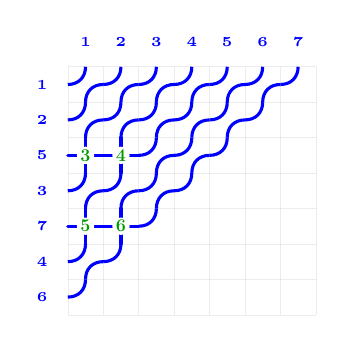
\begin{tikzpicture}[scale=0.45]
  \draw[lightgray, very thin, opacity=0.3] (7,0) -- (0,0);
  \draw[lightgray, very thin, opacity=0.3] (7,0) -- (7,7);
  \draw[lightgray, very thin, opacity=0.3] (7,1) -- (0,1);
  \draw[lightgray, very thin, opacity=0.3] (6,0) -- (6,7);
  \draw[lightgray, very thin, opacity=0.3] (7,2) -- (0,2);
  \draw[lightgray, very thin, opacity=0.3] (5,0) -- (5,7);
  \draw[lightgray, very thin, opacity=0.3] (7,3) -- (0,3);
  \draw[lightgray, very thin, opacity=0.3] (4,0) -- (4,7);
  \draw[lightgray, very thin, opacity=0.3] (7,4) -- (0,4);
  \draw[lightgray, very thin, opacity=0.3] (3,0) -- (3,7);
  \draw[lightgray, very thin, opacity=0.3] (7,5) -- (0,5);
  \draw[lightgray, very thin, opacity=0.3] (2,0) -- (2,7);
  \draw[lightgray, very thin, opacity=0.3] (7,6) -- (0,6);
  \draw[lightgray, very thin, opacity=0.3] (1,0) -- (1,7);
  \draw[lightgray, very thin, opacity=0.3] (7,7) -- (0,7);
  \draw[lightgray, very thin, opacity=0.3] (0,0) -- (0,7);
  \draw[blue, line width=1.125pt] (0,6.5) .. controls (0.3,6.5) and (0.5,6.7) .. (0.5,7);
  \draw[blue, line width=1.125pt] (0.5,6) .. controls (0.5,6.3) and (0.7,6.5) .. (1,6.5);
  \draw[blue, line width=1.125pt] (1,6.5) .. controls (1.3,6.5) and (1.5,6.7) .. (1.5,7);
  \draw[blue, line width=1.125pt] (1.5,6) .. controls (1.5,6.3) and (1.7,6.5) .. (2,6.5);
  \draw[blue, line width=1.125pt] (2,6.5) .. controls (2.3,6.5) and (2.5,6.7) .. (2.5,7);
  \draw[blue, line width=1.125pt] (2.5,6) .. controls (2.5,6.3) and (2.7,6.5) .. (3,6.5);
  \draw[blue, line width=1.125pt] (3,6.5) .. controls (3.3,6.5) and (3.5,6.7) .. (3.5,7);
  \draw[blue, line width=1.125pt] (3.5,6) .. controls (3.5,6.3) and (3.7,6.5) .. (4,6.5);
  \draw[blue, line width=1.125pt] (4,6.5) .. controls (4.3,6.5) and (4.5,6.7) .. (4.5,7);
  \draw[blue, line width=1.125pt] (4.5,6) .. controls (4.5,6.3) and (4.7,6.5) .. (5,6.5);
  \draw[blue, line width=1.125pt] (5,6.5) .. controls (5.3,6.5) and (5.5,6.7) .. (5.5,7);
  \draw[blue, line width=1.125pt] (5.5,6) .. controls (5.5,6.3) and (5.7,6.5) .. (6,6.5);
  \draw[blue, line width=1.125pt] (6,6.5) .. controls (6.3,6.5) and (6.5,6.7) .. (6.5,7);
  \draw[blue, line width=1.125pt] (0,5.5) .. controls (0.3,5.5) and (0.5,5.7) .. (0.5,6);
  \draw[blue, line width=1.125pt] (0.5,5) .. controls (0.5,5.3) and (0.7,5.5) .. (1,5.5);
  \draw[blue, line width=1.125pt] (1,5.5) .. controls (1.3,5.5) and (1.5,5.7) .. (1.5,6);
  \draw[blue, line width=1.125pt] (1.5,5) .. controls (1.5,5.3) and (1.7,5.5) .. (2,5.5);
  \draw[blue, line width=1.125pt] (2,5.5) .. controls (2.3,5.5) and (2.5,5.7) .. (2.5,6);
  \draw[blue, line width=1.125pt] (2.5,5) .. controls (2.5,5.3) and (2.7,5.5) .. (3,5.5);
  \draw[blue, line width=1.125pt] (3,5.5) .. controls (3.3,5.5) and (3.5,5.7) .. (3.5,6);
  \draw[blue, line width=1.125pt] (3.5,5) .. controls (3.5,5.3) and (3.7,5.5) .. (4,5.5);
  \draw[blue, line width=1.125pt] (4,5.5) .. controls (4.3,5.5) and (4.5,5.7) .. (4.5,6);
  \draw[blue, line width=1.125pt] (4.5,5) .. controls (4.5,5.3) and (4.7,5.5) .. (5,5.5);
  \draw[blue, line width=1.125pt] (5,5.5) .. controls (5.3,5.5) and (5.5,5.7) .. (5.5,6);
  \draw[blue, line width=1.125pt, line cap=round] (0,4.5) -- (1,4.5);
  \draw[blue, line width=1.125pt, line cap=round] (0.5,4) -- (0.5,5);
  \draw[blue, line width=1.125pt, line cap=round] (1,4.5) -- (2,4.5);
  \draw[blue, line width=1.125pt, line cap=round] (1.5,4) -- (1.5,5);
  \draw[blue, line width=1.125pt] (2,4.5) .. controls (2.3,4.5) and (2.5,4.7) .. (2.5,5);
  \draw[blue, line width=1.125pt] (2.5,4) .. controls (2.5,4.3) and (2.7,4.5) .. (3,4.5);
  \draw[blue, line width=1.125pt] (3,4.5) .. controls (3.3,4.5) and (3.5,4.7) .. (3.5,5);
  \draw[blue, line width=1.125pt] (3.5,4) .. controls (3.5,4.3) and (3.7,4.5) .. (4,4.5);
  \draw[blue, line width=1.125pt] (4,4.5) .. controls (4.3,4.5) and (4.5,4.7) .. (4.5,5);
  \draw[blue, line width=1.125pt] (0,3.5) .. controls (0.3,3.5) and (0.5,3.7) .. (0.5,4);
  \draw[blue, line width=1.125pt] (0.5,3) .. controls (0.5,3.3) and (0.7,3.5) .. (1,3.5);
  \draw[blue, line width=1.125pt] (1,3.5) .. controls (1.3,3.5) and (1.5,3.7) .. (1.5,4);
  \draw[blue, line width=1.125pt] (1.5,3) .. controls (1.5,3.3) and (1.7,3.5) .. (2,3.5);
  \draw[blue, line width=1.125pt] (2,3.5) .. controls (2.3,3.5) and (2.5,3.7) .. (2.5,4);
  \draw[blue, line width=1.125pt] (2.5,3) .. controls (2.5,3.3) and (2.7,3.5) .. (3,3.5);
  \draw[blue, line width=1.125pt] (3,3.5) .. controls (3.3,3.5) and (3.5,3.7) .. (3.5,4);
  \draw[blue, line width=1.125pt, line cap=round] (0,2.5) -- (1,2.5);
  \draw[blue, line width=1.125pt, line cap=round] (0.5,2) -- (0.5,3);
  \draw[blue, line width=1.125pt, line cap=round] (1,2.5) -- (2,2.5);
  \draw[blue, line width=1.125pt, line cap=round] (1.5,2) -- (1.5,3);
  \draw[blue, line width=1.125pt] (2,2.5) .. controls (2.3,2.5) and (2.5,2.7) .. (2.5,3);
  \draw[blue, line width=1.125pt] (0,1.5) .. controls (0.3,1.5) and (0.5,1.7) .. (0.5,2);
  \draw[blue, line width=1.125pt] (0.5,1) .. controls (0.5,1.3) and (0.7,1.5) .. (1,1.5);
  \draw[blue, line width=1.125pt] (1,1.5) .. controls (1.3,1.5) and (1.5,1.7) .. (1.5,2);
  \draw[blue, line width=1.125pt] (0,0.5) .. controls (0.3,0.5) and (0.5,0.7) .. (0.5,1);
  \node[font=\tiny\bfseries, text=blue, anchor=south] at (0.5,7.3) {1};
  \node[font=\tiny\bfseries, text=blue, anchor=south] at (1.5,7.3) {2};
  \node[font=\tiny\bfseries, text=blue, anchor=south] at (2.5,7.3) {3};
  \node[font=\tiny\bfseries, text=blue, anchor=south] at (3.5,7.3) {4};
  \node[font=\tiny\bfseries, text=blue, anchor=south] at (4.5,7.3) {5};
  \node[font=\tiny\bfseries, text=blue, anchor=south] at (5.5,7.3) {6};
  \node[font=\tiny\bfseries, text=blue, anchor=south] at (6.5,7.3) {7};
  \node[font=\tiny\bfseries, text=blue, anchor=east] at (-0.3,6.5) {1};
  \node[font=\tiny\bfseries, text=blue, anchor=east] at (-0.3,5.5) {2};
  \node[font=\tiny\bfseries, text=blue, anchor=east] at (-0.3,4.5) {5};
  \node[font=\tiny\bfseries, text=blue, anchor=east] at (-0.3,3.5) {3};
  \node[font=\tiny\bfseries, text=blue, anchor=east] at (-0.3,2.5) {7};
  \node[font=\tiny\bfseries, text=blue, anchor=east] at (-0.3,1.5) {4};
  \node[font=\tiny\bfseries, text=blue, anchor=east] at (-0.3,0.5) {6};
  \node[font=\Large\bfseries, text=green!60!black, fill=white, inner sep=0.5pt, circle, transform shape] at (0.5,4.5) {3};
  \node[font=\Large\bfseries, text=green!60!black, fill=white, inner sep=0.5pt, circle, transform shape] at (1.5,4.5) {4};
  \node[font=\Large\bfseries, text=green!60!black, fill=white, inner sep=0.5pt, circle, transform shape] at (0.5,2.5) {5};
  \node[font=\Large\bfseries, text=green!60!black, fill=white, inner sep=0.5pt, circle, transform shape] at (1.5,2.5) {6};
\end{tikzpicture}
} &
\resizebox{0.35\textwidth}{!}{\input{forest_lr_trim.tikz}} \\
$\clp^5(R_i)$ & $\trm^5(R_i)$
\end{tabular}
\caption{Common clip/trim pair for both witnesses $R_1,R_2$.}
\label{fig:forest_lr_cliptrim}
\end{figure}

Therefore Theorem~\ref{theorem:LRforest} gives
$$f_{a,b}^c=2.$$ 
\end{example}


% $$\dsch_u = [\code_1(u)]\dsch_{\downarrow u} - \sum_{\substack{u'\downvar{1} \downarrow u\\ \ell(\downarrow u,u')=\code_1(u)\\u'\neq u}}\dsch_{u'}$$
% where $\downarrow u$ is the unique permutation such that $\code_i(\downarrow u) = \code_{i+1}(u)$.

\section{Product rule for dual slide polynomials}\label{section:slide}
\subsection{Slide polynomials}

\begin{definition}
For a word $\mathbf{r}=\mathbf{r}_1\mathbf{r}_2\cdots \mathbf{r}_k$, a sequences of positive integers $a_1a_2\cdots a_k$ is \emph{compatible} with $\mathbf{r}$ if $a_i\leq \mathbf{r}_i$ for all $i$, $a_i\leq a_{i+1}$ for all $i$, and $a_i<a_{i+1}$ if $\mathbf{r}_i<\mathbf{r}_{i+1}$.

Slide polynomials $\mathfrak{F}(\mathbf{r})$ for a word $\mathbf{r}$ are defined by summing the monomials $x^a$ over all compatible sequences $a$ of $\mathbf{r}$.

Assaf and Searles \cite{assaf2017slide} derived an expansion of Schubert polynomials in terms of slide polynomials as follows. A \emph{quasi-Yamanouchi} RC graph is an RC graph $R$ such that if $R'$ is another RC graph with $\mathrm{word}(R)=\mathrm{word}(R')$ and $\hr(R)=\hr(R')$, then $\wtt(R)\leq \wtt(R')$ in dominance order and $\mathrm{flat}(\wtt(R'))$ refines $\mathrm{flat}(\wtt(R))$. The set of RC graphs $A$ such that $\mathrm{word}(A)=\mathrm{word}(R)$ and $\hr(A)=\hr(R)$ is a partially ordered set with $R$ as its smallest element. We then define
$$\QY(A)=R$$
\end{definition}

\begin{theorem}[{\cite[Theorem~3.13]{assaf2017slide}}]
  For a permutation $w\in S_\infty$, we have the formula
  $$\sch_w(x) = \sum_{R} \mathfrak{F}_{\wtt(R)}(x)$$
  where the sum is over all quasi-Yamanouchi RC graphs $R$ for $w$.
\end{theorem}
% \section{Recursion for Schubert structure constants}
\begin{corollary}
  For a weak composition $c$ of length $p$, we have the formula
  $$\mathfrak{F}_c^* = \sum_{R=\QY(R)} \dsch_{\wof{R}}^p$$
  where the sum is over all quasi-Yamanouchi RC graphs $R$ such that $\wtt(R) = c$.
\end{corollary}

% $$\sum_{R\in\RC(c)\atop R=\QY(R)} \Delta(\dsch_{\wof{R}}^p) = \Delta(\mathfrak{F}_c^*)$$

% $$\sum_{R\in\RC(c)\atop R=\QY(R)} c_{u,v}^{\wof{R}}\dsch_u^p\otimes \dsch_v^p = \mathrm{shuff}_{a,b}^c\mathfrak{F}_a^*\otimes\mathfrak{F}_b^*$$

% $$\sum_{R\in\RC(c)\atop R=\QY(R)} c_{u,v}^{\wof{R}}\dsch_u^p\otimes \dsch_v^p = \mathrm{shuff}_{a,b}^c\sum_{A\in\RC(u,a)\atop A=\QY(A)}\sum_{B\in\RC(v,b)\atop B=\QY(B)}\dsch_{u}^p\otimes\dsch_{v}^p$$

% $$\sum_{R\in\RC(c)\atop R=\QY(R)} c_{u,v}^{\wof{R}}=\mathrm{shuff}_{a,b}^c\#\{A\in\RC(u,a)\mid A=\QY(A)\}\#\{B\in\RC(v,b)\mid B=\QY(B)\}$$

\begin{definition}
For a weak composition $c$, define $\RC_\QY(c)$ to be the set of RC graphs with $\wtt(R) = c$ such that $\mathrm{word}(\QY(R))$ is minimal in lexicographical order among all RC graphs $R'$ with $\wtt(\QY(R')) = \wtt(\QY(R))$. 
\end{definition}

\begin{proposition}
Let $c$ be a weak composition of length $p$.
$$[c] = \sum_{R\in\RC_\QY(c)} \mathfrak{F}_{\wtt(\QY(R))}^*$$
\end{proposition}

\begin{definition}[The submodule $\Sigma\subseteq \BRC$]
Let $\Sigma$ be the $\mathbb{Z}$-submodule of $\BRC$ generated by the elements $R_1-R_2$ such that $\QY(R_1)=\QY(R_2)$.
\end{definition}

\begin{lemma}\label{lemma:slideideal}
$\Sigma$ is a two-sided ideal of $\BRC$.
\end{lemma}
\begin{proof}
That $\Sigma$ is a left ideal follows from the same mechanism used for $\Theta$: in $R\sqcupplus R_1$ and $R\sqcupplus R_2$, the first $\hr(R)$ rows agree, while the trailing rows are shifts of $R_1$ and $R_2$. Since the crystal operators act on adjacent rows, they descend in the same way to the trailing block. The quasi-Yamanouchi map $\QY$ is defined by applying a sequence of crystal raising operators determined by the weight (\cite{assaf2017slide}); hence applying $\QY$ to $R\sqcupplus R_1$ and to $R\sqcupplus R_2$ produces graphs whose trailing rows have a common partial quasi-Yamanouchi reduction $R\sqcupplus \QY(R_1)=R\sqcupplus \QY(R_2)$, and so $\QY(R\sqcupplus R_1)=\QY(R\sqcupplus R_2)$.

That $\Sigma$ is a right ideal follows from Corollary \ref{corollary:crystaliso}: multiplication on the right by a fixed $R$ induces an isomorphism of crystal graphs on the relevant subblock, and the $\QY$ images of corresponding terms therefore agree.
\end{proof}

\begin{lemma}
The homomorphism $\alpha:\BRC\to\dcoma$ factors through the quotient $\BRC/\Sigma$.
\end{lemma}
\begin{proof}
This is because the generators of $\Sigma$ are all in $\Omega$: if $\QY(R_1)=\QY(R_2)$ then $\wof{R_1}=\wof{\QY(R_1)}=\wof{\QY(R_2)}=\wof{R_2}$ and $\hr(R_1)=\hr(R_2)$, so $\alpha(R_1)=\alpha(R_2)$.
\end{proof}

\begin{definition}
For a weak composition $a$, define an element $\mathcal{F}_a\in\BRC/\Sigma$ by
$$\mathcal{F}_a=\sum_{R: \QY(R)=R,\ \wtt(R)=a} R.$$
\end{definition}

\begin{proposition}\label{proposition:slidebasis}
The elements $\mathcal{F}_a\in\BRC/\Sigma$ form an additive basis of a subring isomorphic to $\dcoma$ under the homomorphism $\alpha:\BRC/\Sigma\to\dcoma$, and
$$\alpha(\mathcal{F}_a)=\mathfrak{F}_a^*.$$
\end{proposition}
\begin{proof}
The last identity is the Corollary above. Distinct $\mathcal{F}_a$ are supported on disjoint sets of quasi-Yamanouchi RC graphs (indexed by their common weight $a$), so the $\mathcal{F}_a$ are linearly independent in $\BRC/\Sigma$. Considering the homomorphism $\alpha:\BRC/\Sigma\to\dcoma$, since the $\mathfrak{F}_a^*$ are linearly independent, the kernel of $\alpha$ intersects the span of the $\mathcal{F}_a$ trivially; hence $\alpha$ is injective on $\sum_a \mathbb{Z}\mathcal{F}_a$. Since
$$\alpha(\mathcal{F}_a)\sqcupplus\alpha(\mathcal{F}_b)=\mathfrak{F}_a^*\sqcupplus\mathfrak{F}_b^*=\sum_c s_{a,b}^c\,\mathfrak{F}_c^*=\sum_c s_{a,b}^c\,\alpha(\mathcal{F}_c),$$
the product $\mathcal{F}_a\sqcupplus\mathcal{F}_b$ lies in the span of the $\mathcal{F}_c$, so this span is closed under multiplication and the restriction of $\alpha$ is a ring isomorphism.
\end{proof}

\begin{theorem} \label{theorem:lrfslide}
  Let $a,b$ be weak compositions of lengths $p$ and $q$. Write
$$\mathfrak{F}_a^*\sqcupplus\mathfrak{F}_b^*=\sum_c s_{a,b}^c\,\mathfrak{F}_c^*$$
For each $c$, fix an RC graph $C$ with $\wtt(\QY(C)) = c$. Then $s_{a,b}^c$ is the number of distinct RC graphs $R$ with $\mathrm{word}(R)=\mathrm{word}(C)$ with $\wtt(\clp^p(R)) = a,\wtt(\trm^p(R)) = b$ such that $\clp^p(R),\trm^p(R)$ are quasi-Yamanouchi, and is in particular nonnegative.
\end{theorem}
\begin{proof}
The coefficient of $\mathcal{F}_c$ in $\mathcal{F}_a\sqcupplus\mathcal{F}_b$ equals the coefficient of $\mathfrak{F}_c^*$ in $\mathfrak{F}_a^*\sqcupplus\mathfrak{F}_b^*$, namely $s_{a,b}^c$, by Proposition \ref{proposition:slidebasis}. Expanding the product $\mathcal{F}_a\sqcupplus\mathcal{F}_b$ via the $(\clp^p,\trm^p)$-decomposition of $\sqcupplus$ (Theorem \ref{theorem:modactrc}) and reading off the coefficient of $\mathcal{F}_c$ from a fixed representative $C$ with $\wtt(\QY(C))=c$, the contributing terms are precisely the RC graphs $R$ with $\mathrm{word}(R)=\mathrm{word}(C)$ whose clip and trim have quasi-Yamanouchi weights $a$ and $b$ respectively.
\end{proof}

\subsection{A general ideal-quotient Littlewood--Richardson principle}

The dual Schubert, dual key, and dual forest LR rules of the previous sections all fit a common template, which we record here.

\begin{theorem}[General LR principle via ideals of $\BRC$]\label{theorem:general_lr_template}
Let $\sim$ be an equivalence relation on $\bigsqcup_n \RC_n$ satisfying:
\begin{itemize}
\item[(H1)] If $R_1\sim R_2$ then $\hr(R_1)=\hr(R_2)$ and $\wof{R_1}=\wof{R_2}$ (in particular $\alpha(R_1)=\alpha(R_2)$).
\item[(H2)] $\sim$ is a congruence for $\sqcupplus$: $R_1\sim R_2$ implies $R\sqcupplus R_1\sim R\sqcupplus R_2$ and $R_1\sqcupplus R\sim R_2\sqcupplus R$ for every $R$.
\item[(H3)] $\clp^p$ and $\trm^p$ descend to $\sim$: if $R_1\sim R_2$ and $1\leq p\leq \hr(R_1)$, then $\clp^p(R_1)\sim \clp^p(R_2)$ and $\trm^p(R_1)\sim \trm^p(R_2)$.
\item[(H4)] There is an index set $J$ and a function $\lambda:(\RC/\!\sim)\to J$ such that, writing $I_\sim=\mathrm{span}_{\mathbb{Z}}\{R_1-R_2:R_1\sim R_2\}\subseteq\BRC$ and
$$E_\lambda := \sum_{[R]:\,\lambda([R])=\lambda} [R] \in \BRC/I_\sim,$$
the family $\{\alpha(E_\lambda)\}_{\lambda\in J}$ is a $\mathbb{Z}$-basis of $\dcoma$.

\end{itemize}
Then $I_\sim$ is a two-sided ideal of $\BRC$ contained in $\Omega=\ker\alpha$, the elements $\{E_\lambda\}$ span a subring of $\BRC/I_\sim$ isomorphic to $\dcoma$ via $\alpha$, and the structure constants $b_{\mu,\nu}^\lambda$ defined by
$$\mathfrak{B}_\mu^*\sqcupplus\mathfrak{B}_\nu^* = \sum_\lambda b_{\mu,\nu}^\lambda\,\mathfrak{B}_\lambda^*,\qquad \mathfrak{B}_\lambda^*:=\alpha(E_\lambda),$$
are nonnegative integers. More precisely, for any function $\mathrm{rep}\colon\RC\to\RC$ that sends every element of a $\sim$-class to a single common representative of that class (that is, $\mathrm{rep}(R)\sim R$ for all $R$, and $\mathrm{rep}(R)=\mathrm{rep}(S)$ whenever $R\sim S$), we have the positive combinatorial formula
\begin{align*}
b_{\mu,\nu}^\lambda \;=\; \#\bigl\{\,R\sim C\ :\ &\clp^p(R)=\mathrm{rep}(\clp^p(R)),\;\;\trm^p(R)=\mathrm{rep}(\trm^p(R)),\\
&\lambda([\clp^p(R)])=\mu,\;\;\lambda([\trm^p(R)])=\nu\,\bigr\}
\end{align*}
for any fixed $C$ with $\lambda([C])=\lambda$. The count is independent of the choice of $\mathrm{rep}$.
\end{theorem}
\begin{proof}
By (H1) every generator $R_1-R_2$ of $I_\sim$ lies in $\Omega=\ker\alpha$, so $I_\sim\subseteq\Omega$ and $\alpha$ descends to a surjective ring homomorphism $\overline\alpha:\BRC/I_\sim\to\dcoma$. By (H2), $I_\sim$ is a two-sided ideal of $\BRC$, so $\BRC/I_\sim$ inherits a ring structure.

By construction of $E_\lambda$ in (H4), each $\sim$-class $[R]$ appears in $E_\lambda$ with multiplicity exactly $1$ (when $\lambda([R])=\lambda$) or $0$ (otherwise), and the supports of $E_\lambda$ and $E_{\lambda'}$ in $\BRC/I_\sim$ are disjoint whenever $\lambda\neq\lambda'$; consequently the coefficient $b_{\mu,\nu}^\lambda$ may be read off from the contribution to a single chosen class $[C]$ with $\lambda([C])=\lambda$. In particular the $\{E_\lambda\}$ are linearly independent. Under $\overline\alpha$ they map to the $\mathbb{Z}$-basis $\{\mathfrak{B}_\lambda^*\}$ of $\dcoma$ by (H4), so $\overline\alpha$ restricts to a $\mathbb{Z}$-module isomorphism $\bigoplus_\lambda\mathbb{Z}E_\lambda\xrightarrow{\;\cong\;}\dcoma$. Since $\overline\alpha$ is a ring homomorphism, the span of the $E_\lambda$ is closed under multiplication and the isomorphism is one of rings. Consequently
$$E_\mu \sqcupplus E_\nu = \sum_\lambda b_{\mu,\nu}^\lambda\, E_\lambda \quad\text{in } \BRC/I_\sim.$$

To read off $b_{\mu,\nu}^\lambda$, fix any $C$ with $\lambda([C])=\lambda$ and let $S_1=\mathrm{rep}(R_1)$, $S_2=\mathrm{rep}(R_2)$ be the chosen representatives of the $\mu$- and $\nu$-classes (for any $R_1,R_2$ in those classes). By Theorem~\ref{theorem:modactrc} the product $\sqcupplus$ on $\BRC$ admits a $(\clp^p,\trm^p)$-decomposition: for any $S_1,S_2$ with $\hr(S_1)=p$, $\hr(S_2)=q$, the set $\{R\in\RC_{p+q}:\clp^p(R)=S_1,\,\trm^p(R)=S_2\}$ enumerates the summands of $S_1\sqcupplus S_2$ with multiplicity one. Projecting to $\BRC/I_\sim$, (H3) ensures that the class of $R$ depends only on the classes of $\clp^p(R)$ and $\trm^p(R)$, so the contribution of $S_1\sqcupplus S_2$ to the coefficient of $[C]$ in $E_\lambda$ is exactly the count of $R\sim C$ for which $\clp^p(R)=S_1$ and $\trm^p(R)=S_2$, i.e.\ for which $\clp^p(R)$ and $\trm^p(R)$ are themselves fixed points of $\mathrm{rep}$ and represent the $\mu$- and $\nu$-classes. This is the stated formula. Being a cardinality, it is nonnegative.

Finally, the count is independent of the choice of $\mathrm{rep}$. The element $E_\lambda\in\BRC/I_\sim$ is defined directly as $\sum_{[R]:\lambda([R])=\lambda}[R]$, with no reference to $\mathrm{rep}$, so the structure constants in $E_\mu E_\nu=\sum_\lambda b_{\mu,\nu}^\lambda E_\lambda$ are intrinsic. To see that the formula computes the correct value for every valid $\mathrm{rep}$, fix classes $[T_1],[T_2]$ with $\lambda([T_1])=\mu$, $\lambda([T_2])=\nu$, and consider, for any $S_1\in[T_1]$ and $S_2\in[T_2]$, the count
$$N(S_1,S_2):=\#\{R\sim C\,:\,\clp^p(R)=S_1,\ \trm^p(R)=S_2\}.$$
By the $(\clp^p,\trm^p)$-decomposition of Theorem~\ref{theorem:modactrc}, $N(S_1,S_2)$ equals the coefficient of $[C]$ in the product $[S_1]\sqcupplus[S_2]\in\BRC/I_\sim$ (using (H2) to make the product well-defined and (H3) to ensure each summand of $S_1\sqcupplus S_2$ has $\sim$-class depending only on $[S_1]$ and $[S_2]$). In particular $N(S_1,S_2)$ depends only on the classes $[T_1],[T_2]$ and on $[C]$, not on the choice of representatives $S_1,S_2$. The $\mathrm{rep}$-formula selects, for each such class-pair, the single representative pair $(\mathrm{rep}(T_1),\mathrm{rep}(T_2))$ and counts $N(\mathrm{rep}(T_1),\mathrm{rep}(T_2))$; another valid $\mathrm{rep}'$ counts $N(\mathrm{rep}'(T_1),\mathrm{rep}'(T_2))$, and these are equal. Summing over class-pairs yields the same total $b_{\mu,\nu}^\lambda$.
\end{proof}

\begin{remark}\label{remark:general_lr_instances}
In the present paper, Theorem~\ref{theorem:general_lr_template} is instantiated by
\begin{itemize}
\item $\sim$ = equality on $\RC$, with $I_\sim=0$ and $\lambda([R])=(\wof{R},\hr(R))$, recovering Theorem~\ref{theorem:LR} (dual Schubert basis);
\item $\sim$ = Demazure-crystal equivalence, with $I_\sim=\Theta$ and $\lambda$ the extremal weight, recovering Theorem~\ref{theorem:LRkey} (dual key basis);
\item $\sim\,=\,\equiv_\forest$, with $I_\sim=\Gamma$ and $\lambda=\fcode$, recovering Theorem~\ref{theorem:LRforest} (dual forest basis);
\item $\sim$ = ``same reduced word and same $\hr$'' on $\RC$, with $\lambda([R])=\wtt(\QY(R))$, recovering Theorem~\ref{theorem:lrfslide} (dual slide basis).
\end{itemize}
The verifications of (H1)--(H4) in each case are precisely the lemmas and propositions of \S\ref{section:bialgebra}, \S\ref{section:crystals}, \S\ref{section:forest}, and \S\ref{section:slide}.
\end{remark}

\section{The Littlewood-Richardson rule for forest polynomials}\label{section:forestrule}

\subsection{The multiplactic algebra}
\begin{definition}
Let $R_1$ and $R_2$ be RC graphs with $\hr(R_1)=\hr(R_2)$. Let $N$ be the position of the last unfixed point of $\wof{R_1}$. We define
$$R_1\sqcup R_2 = R_1\cup \{(i,j+N)\mid (i,j)\in R_2\}$$
This is an RC graph with $|R_1\sqcup R_2| = |R_1| + |R_2|$ and $\hr(R_1\sqcup R_2)=\hr(R_1) + N$, though at most only the first $\hr(R_1)$ rows are occupied.  It is not too difficult to see that
$$\wof{R_1\sqcup R_2} = \wof{R_1}\shup^{N}\wof{R_2}$$

We then define the \emph{squash product} of $R_1$ and $R_2$ to be
$$R_1\boxtimes R_2 = \clp^{\hr(R_1)}(R_1\sqcup R_2)$$

\end{definition}

\begin{proposition} \label{proposition:boxproduct}
  Let $u\in S_\infty$ be a permutation such that $\maxd(u)\leq n$ and let $v$ be an $n$-Grassmannian permutation. Then we have that
  $$\boxtimes:\RC_n(u)\otimes \RC_n(v)\to \bigoplus_{w\in S_\infty} \RC_n(w)^{\oplus c_{uv}^w}$$
  is an isomorphism of crystal graphs. 
\end{proposition}
\begin{proof}
Clearly the map is weight preserving. We defer the assertion that the image is precisely correct by allowing us to expand the codomain to the set $\RC_n$. 
%The fact that it is a bijection is  for this, we must invoke \cite{tuono2020decomposition}. 
Let us show that the function commutes with the crystal operators. Let $R_1\in \RC_n(u)$ and $R_2\in \RC_n(v)$, and let $R=R_1\sqcup R_2$. Consider $f_i(R_1\otimes R_2)$. If $\varphi_i(R_1)>\varepsilon_i(R_2)$, then the unpaired elements in row $i$ in $R_1$ exhaust the unpaired elements in row $i+1$ in $R_2$. Therefore, only elements of $R_1$ are affected by $f_i$, as in the definition of the tensor product. If instead $\varphi_i(R_1)\leq \varepsilon_i(R_2)$, then all unpaired elements of $R_1$ in row $i$ are paired with elements of $R_2$ in row $i+1$, and so only elements of $R_2$ are affected by $f_i$. The same reasoning applies to $e_i$. The fact that the isomorphism induces the specific decomposition follows from \cite{kouno2020decomposition}.
\end{proof}

\begin{definition}
We define an RC graph $R$ of $\hr(R)=k$ to be \emph{full Grassmannian} if $\wof{R}$ is a $k$-Grassmannian permutation. We define $\grass_n$ to be the $\mathbb{Z}$-submodule of $\BRC_n$ generated by all full Grassmannian RC graphs with $\hr(R)= n$.

We define $\plac_n$ to be the plactic algebra on $[n]$, the free abelian group on the set of words in $[n]$ modulo the Knuth relations. We take as the basis of $\plac_n$ the set of row reading words of semistandard Young tableaux \emph{in French notation} (upside-down).

Consider the set $I(v)$ of right inversions of an $n$-Grassmannian permutation $v$, that is to say the pairs $(i,j)$ with $i<j$ and $v(i)>v(j)$. An RC graph $R\in\RC_n(v)$ corresponds bijectively to a labeling $T_R:I(v)\to [n]$ by defining
$$T_R(\rtt(i,j)) = i$$
for an element $(i,j)\in R$ (see, for example, \cite{axelrodfreed2025inversionstableaux}). If $R_0$ is the bottom RC graph of $v$, then there is a bijection between the elements of $I(v)$ and the boxes of the Young diagram of $v$ given by
$$(i,j) \mapsto (i + \ell(\mathrm{shape}(v)) - n, j)$$
Hence there is a linear isomorphism
$$P_n:\mathrm{SSYT}(n)\to \grass_n$$
sending $T$ to the RC graph $R$ such that $T_R = T$.
\end{definition}

\begin{lemma}
Suppose $R$ is full $n$-Grassmannian such that all rows after row $r$ for some $r\leq n$ are empty. Then $\clp^r(R)$ is full $r$-Grassmannian, and if $T\in \SSYT(n)$ satisfies $P_n(T)=R$, then $P_r(T)=\clp^r(R)$.
\end{lemma}
\begin{proof}
From Theorem \ref{theorem:zero_bijection} and the fact that Schur polynomials are stable, we have that $\clp^r(R)$ is full $r$-Grassmannian of the same shape and weight. Invoking the more specific Theorem \ref{theorem:zerocrystal} and theory of Kashiwara crystals, we have that $P_r(T)=\clp^r(R)$.
\end{proof}

\begin{theorem} \label{theorem:placticiso}
We have that the bilinear map $\boxtimes: \grass_n\times \grass_n\to\grass_n$ is an associative product such that $P_n:\plac_n\to \grass_n$ is an isomorphism of rings.
\end{theorem}
\begin{proof}
Consider the function 
$$\tau_n:\plac_n\otimes \plac_n\to \bigoplus_{N = n}^\infty \BRC_N$$ 
defined on basis elements by
$$\tau_n(T_1\otimes T_2) = P_n(T_1)\sqcup P_n(T_2)$$
Proposition \ref{proposition:boxproduct} shows that
$$\clp^n(\tau_n(T_1\otimes T_2)) = P_n(T_1)\boxtimes P_n(T_2) = P_n(T_1T_2)$$
due to the rigidity of crystal graph isomorphisms. Since $P_n$ is therefore a homomorphism of (potentially nonassociative) algebras as well as bijective, it is an isomorphism, from which it follows that $\boxtimes$ itself is associative.
\end{proof}

\begin{theorem} \label{theorem:schubmoduleiso}
  The module $\BRC_n$ is a right $\grass_n$-module under the product $\boxtimes$. Considering $\BRC_n$ as a right module over $\Lambda_n$ via the injective homomorphism $\Lambda_n\hookrightarrow \plac_n\simeq \grass_n$, the $\Lambda_n$-submodule generated by $\mathcal{S}_w(n)$ for $w\in S_n$ is isomorphic to the polynomial ring $\mathbb{Z}[x_1,\ldots,x_n]$ as a $\Lambda_n$-module via the homomorphism $\mathcal{S}_w(n)\mapsto\sch_w(x)$, and in particular is a free right $\Lambda_n$-module with basis $\{\mathcal{S}_w(n)\mid w\in S_n\}$.
\end{theorem}
\begin{proof}
The fact that $\BRC_n$ is a right $\grass_n$ module follows from Proposition \ref{proposition:boxproduct} and the statement that the tensor product of crystal graphs is associative. The injective homomorphism of rings $\Lambda_n\hookrightarrow \plac_n\simeq \grass_n$ is given by sending a Schur polynomial $s_\lambda$ to the sum of all words of semistandard tableaux of shape $\lambda$ is realized through $P_n$. The map $\BRC_n\to \mathbb{Z}[x_1,\ldots,x_n]$ sending $R$ to $x^{\wtt(R)}$ is clearly a surjective homomorphism of abelian groups. Restricting to the submodule $\mathrm{Schub}_n$, since $\mathcal{S}_w(n)\mapsto \sch_w^n(x)$ for all $w$ with $\maxd(w)\leq n$, we obtain an isomorphism of $\mathbb{Z}$-modules at the very least. Proposition \ref{proposition:boxproduct} ensures that the restriction to this submodule is in fact a $\Lambda_n$-isomorphism. Thus, the $\Lambda_n$-submodule generated by the $\mathcal{S}_w(n)$ is free with basis $\{\mathcal{S}_w(n)\mid w\in S_n\}$.
\end{proof}

\begin{definition}
Consider the ring $\mathcal{M}_n$ defined as
$$\mathcal{M}_n = \bigotimes_{k=1}^n \grass_k$$
%where $\sim$ is the equivalence relation generated by the following:
%the multiplactic algebra on the free abelian groups generated by the set of full $k$-Grassmannian elementary symmetric polynomial RC graphs (i.e. single columns), satisfying the additional condition that if $ A\otimes B$ are such that $\hr(A)\neq \hr(B)$, then

We then define a linear homomorphism
$$\mathcal{M}_n\to \BRC_n$$
by
$$\RC(A_1\otimes A_2\otimes \cdots \otimes A_k) = A_1\boxtimes A_2\boxtimes \cdots \boxtimes A_k$$
where we increase the size of the left factor to match the right factor as needed, finally resizing the end result to height $n$.

We may avoid the clunky tensor product notation by noting that we may identify which tensor factor an element of $\mathcal{M}_n$ belongs to by its height, and so we may write elements of $\mathcal{M}_n$ as formal products of full-Grassmannian RC graphs, with the understanding that the $k$-th factor of the product is the submodule $\grass_k$.

Define $\mathbf{E}_{p}^k$ to be the sum of all full $k$-Grassmannian elementary symmetric polynomial RC graphs of degree $p$, considered as an element of $\mathcal{M}_n$.
\end{definition}

\begin{proposition} \label{proposition:eproductworks}
For any $p_1,p_2,\ldots,p_m$ and $k_1\leq k_2\leq\ldots\leq k_m\leq n$ with $p_i\leq k_i$ for all $i$, we have that
$$\RC_n(\mathbf{E}_{p_1}^{k_1}\mathbf{E}_{p_2}^{k_2}\cdots\mathbf{E}_{p_m}^{k_m}) = \sum_{w} c_w\mathcal{S}_w(n)$$
where $c_w\in \mathbb{Z}_{\geq 0}$ are the coefficients such that
$$e_{p_1,k_1}^n\cdots e_{p_m,k_m}^n = \sum_w c_w \sch_w^n(x)\in \coma_n$$
\end{proposition}
\begin{proof}
We prove this by induction on $m$. For an elementary tensor $A_1\otimes \cdots \otimes A_m$, the result follows directly from the definition of $\RC_n$. Assuming the inductive hypothesis that this formula holds for tensors of length less than $m$, then for a tensor of length $m$ we have that
$$\RC_n(\mathbf{E}_{p_1}^{k_1}\mathbf{E}_{p_2}^{k_2}\cdots\mathbf{E}_{p_m}^{k_m}) = \RC_n(\mathbf{E}_{p_1}^{k_1}\mathbf{E}_{p_2}^{k_2}\cdots\mathbf{E}_{p_{m-1}}^{k_{m-1}})\boxtimes \RC_n(\mathbf{E}_{p_m}^{k_m})=\sum_{w'} c_{w'}' \mathcal{S}_{w'}(n)\boxtimes \mathbf{E}_{p_m}^{k_m}$$
by Theorem \ref{theorem:schubmoduleiso}, since $\mathbf{E}_{p_m}^{k_m}\in\grass_{k_m}$, and we are ensured by the increasing order of $k_i$ that the left factor can be clipped to height $k_m$ without the permutation changing. We then apply Proposition \ref{proposition:boxproduct} to obtain the result for a single term of this type by induction. Invoking the fact that the image lies in $\mathrm{Schub}_n$, the result follows by applying Theorem \ref{theorem:schubmoduleiso}.
\end{proof}

% We impose further relations as follows. Suppose we have $A\otimes B$, where $\hr(A)=\hr(B)$ and $A$ and $B$ are both full Grassmannian. If $\hr(A) = n$, then we use $A\boxtimes B$ as the relation of equality. If $\hr(A)<n$, compute the RC graph
% $$R = A\boxtimes B$$
% If this is elementary symmetric, declare
% $$A\otimes B = R$$
% Otherwise,
% $$R\in \RC_k(w)$$
% for some $w\notin S_k$.
% \begin{theorem} \label{theorem:productworks}
% The projection $\mathcal{M}_n\to \mathbb{Z}[x_1,\ldots,x_n]$ is a surjective homomorphism of rings such that the subring generated by the $\mathbf{E}_{p,k}^n$ factors via $\RC$ through the isomorphism of $\Lambda_n$-modules $\mathbb{Z}\mathcal{S}_w(n)\to\mathbb{Z}[x_1,\ldots,x_n]$ sending $\mathcal{S}_w(n)$ to $\sch_w(x)$.
% \end{theorem}
% \begin{proof}

% \end{proof}

\begin{definition}
  Suppose $\maxd(w)\leq n$. We define an element $\mathbf{S}_w(n)\in \mathcal{M}_n$ by
  $$\mathbf{S}_w(n) = \sum_{\alpha} E_w^{\alpha;n}\mathbf{E}_{\alpha_1,1}^1 \mathbf{E}_{\alpha_2,2}^2 \cdots  \mathbf{E}_{\alpha_n,n}^n\mathbf{E}_{\alpha_{n+1}, n}^n\cdots \mathbf{E}_{\alpha_N,n}^n$$
\end{definition}

\begin{theorem} \label{theorem:schubproduct}
Let $u,v\in S_\infty$ satisfy $\maxd(u),\maxd(v)\leq n$. Then
$$\RC_n(\mathbf{S}_u(n)\mathbf{S}_v(n)) = \sum_{w} c_{uv}^w \mathcal{S}_w(n)$$
where $c_{uv}^w$ are the Schubert structure constants.
\end{theorem}
\begin{proof}
  Explicitly, write
  $$\mathbf{S}_u(n)\mathbf{S}_v(n) = \sum_{\alpha,\beta} E_u^{\alpha;n}E_v^{\beta;n} \mathbf{E}_{\alpha_1,1}^1 \cdots  \mathbf{E}_{\alpha_N,n}^n \mathbf{E}_{\beta_1,1}^1 \cdots  \mathbf{E}_{\beta_N,n}^n$$
  The relations of the ring allow us to slide smaller terms in $\mathbf{S}_v(n)$ past strictly larger terms in $\mathbf{S}_u(n)$, so we may rearrange the product in increasing order of height. The result then follows from Proposition \ref{proposition:eproductworks} and the fact that the image of the element under $\RC_n$ lies in $\mathrm{Schub}_n$, so that we may invoke Theorem \ref{theorem:schubmoduleiso}.
\end{proof}

\begin{remark}
It may be unsurprising to the reader at this point that the kernel of $\RC_n:\mathcal{M}_n\to \BRC_n$ \emph{is not an ideal}. If it were, then the product on $\mathcal{M}_n$ would descend to a term by term product such that
$$\mathcal{S}_u(n)\cdot \mathcal{S}_v(n) = \sum_{w} c_{uv}^w \mathcal{S}_w(n)$$
and the problem of finding a positive formula for the Schubert structure constants would be solved, due to the fact that $\mathcal{S}_u(n)$ and $\mathcal{S}_v(n)$ have completely nonnegative coefficients. Unfortunately, this is simply not true. The negative terms in $\mathcal{S}_u(n)$ are essential in making the product work.
\end{remark}

% \begin{example}[Descending to the RC graph level: not associative]

% \end{example}

\subsection{The lift product}\label{section:liftproduct}

We now define a product on $\BRC_n$ that is associative, but as necessitated by the remark above does not correctly model Schubert polynomial multiplication. However, we will see that it is correct enough to give a Littlewood-Richardson rule for forest polynomials.

\begin{proposition} \label{proposition:elemfactor}
  Let $u\in S_\infty$ be a permutation and suppose $R\in \RC_n(u)$. Let $\lambda$ be a partition and let $w$ be the corresponding dominant permutation with $\code^*(w)=\lambda$. Assume that $\ell(uw^{-1}) = \ell(w)-\ell(u)$. Let $c$ be a composition such that $c_i\leq \lambda_{N + 1 - i}$ for all $i$, where $N=\ell(\lambda)$. Then the number of sequences of elementary symmetric RC graphs $A_1,\ldots,A_N$ such that $|A_i| = c_i$ and $\hr(A_i) = \lambda_{N + 1 - i}$ satisfying
  $$A_1\boxtimes\cdots\boxtimes A_N = R$$
is equal to the coefficient of $x^c$ in $\sch_{uw^{-1}}(x)$.
\end{proposition}
\begin{proof}
  Recall the Cauchy formula for $\sch_w(x;-y)$:
  $$\sch_w(x;-y)=\sum_u \sch_u(x)\sch_{uw^{-1}}(y)$$
  Also,
  $$\sch_w(x;-y) = E_{\lambda_1,\lambda_1}(x;-y_1)\cdots E_{\lambda_N,\lambda_N}(x;-y_N)$$

Replace the factorial elementary symmetric polynomial $E_{p,p}(x;-y_i)$ for each $p$ with $\mathbf{E}_p^p(-y_i)\in \mathcal{M}_n[y_1,\ldots,y_N]$ defined by
$$\mathbf{E}_p^p(-y_i) = \sum_{j=0}^p y_i^j \mathbf{E}_{p-j}^p$$
The result follows from Proposition \ref{proposition:eproductworks}.
\end{proof}



\begin{definition}
  Define a function $\mathrm{lift}_n:\RC_n\to \mathcal{M}_n$ as follows. For an RC graph $R\in \RC_n$, let $\lambda$ be a partition of the form 
$$(\overbrace{n,\ldots,n}^{p},n-1,n-2,\ldots,1)$$
where $p$ is sufficiently large such that if $\mu$ is the dominant permutation with $\code^*(\mu)=\lambda$, then $\ell(\wof{R}\mu^{-1}) = \ell(\mu) - \ell(\wof{R})$.  Let $c$ be the code of the permutation $\wof{R}\mu^{-1}$. Then we define
$$\mathrm{lift}_n(R) = E_1 \cdots  E_{\ell(c)}$$
where $|E_i| = \lambda_{N + 1 - i} - c_{N + 1 - i}$ and $\hr(E_i) = \lambda_{N+1-i}$ for all $i$, with $E_i$ all elementary symmetric full Grassmannian RC graphs, which is guaranteed to exist and be unique by Proposition \ref{proposition:elemfactor}. 
\end{definition}

Some justification that $\mathrm{lift}_n$ is well-defined is in order. For each choice of $\lambda$, the existence and uniqueness of the factorization follows from Proposition \ref{proposition:elemfactor}. However, $\lambda$ depends on a choice of $p$ ``sufficiently large.'' We must show that the factorization is independent of this choice. If we increase $p$ by one, then $\lambda$ is replaced by $\lambda' = (\overbrace{n,\ldots,n}^{p+1},n-1,n-2,\ldots,1)$. The code of $\wof{R}(\mu')^{-1}$ is then obtained from the code of $\wof{R}\mu^{-1}$ by prepending $n$, so the same factorization works for both choices of $p$.

\begin{definition}
We define a product $*$ on $\BRC_n$ by
$$R_1*R_2 = \RC_n(\mathrm{lift}_n(R_1)\mathrm{lift}_n(R_2))$$
\end{definition}

%Such a tensor $A_1\otimes\cdots\otimes A_n$ is highest weight if for each $i,j$ we have that either there is a crossing in row $j+1$ but none in row $j$ in $A_i$, or there is no crossing in row $j$ in $A_{i+1}$,  or there are crossings in both rows $j$ and $j+1$ in $A_{i+1}$.
\begin{lemma}
  Let $R$ be an RC graph and suppose
$$\mathrm{lift}_n(R) = A_1\cdots A_n$$
Let $1\leq j\leq n$ and let 
$$R^{\mathrm{left}} = \RC_n(A_1\cdots  A_j)$$
and
$$R^{\mathrm{right}} = \RC_n(A_{j+1}\cdots  A_n)$$
Then
$$\mathrm{lift}_n(R^{\mathrm{left}}) = A_1\cdots  A_j$$
and
$$\mathrm{lift}_n(R^{\mathrm{right}}) = A_{j+1}\cdots  A_n$$
\end{lemma}
\begin{proof}
This follows from the fact that if a partition $\lambda$ is split into an initial section $\lambda_1$ of length $n-j$ and a final section $\lambda_2$ of length $j$, if we define $w_1$ and $w_2$ to be the dominant permutations with $\code^*(w_i)=\lambda_i$, and if we define $c_1$ and $c_2$ to be the codes of $\wof{R^{\mathrm{left}}}w_1^{-1}$ and $\wof{R^{\mathrm{right}}}w_2^{-1}$, then the code of $\wof{R}(w_1w_2)^{-1}$ is obtained by concatenating $c_1$ and $c_2$. The result then follows from Proposition \ref{proposition:elemfactor}.
\end{proof}

\begin{lemma}[Lift factors at disjoint height ranges commute]\label{lemma:liftcommute}
Let $A\in\mathcal{M}_n$ be a tensor of elementary RC factors all of whose heights are at most $k$, and let $B\in\mathcal{M}_n$ be a tensor of elementary RC factors all of whose heights are strictly greater than $k$. Then
$$A\cdot B = B\cdot A\qquad\text{in }\mathcal{M}_n,$$
where the product is the lift product $*$ on $\BRC_n$ transferred to $\mathcal{M}_n$ via $\mathrm{lift}_n$. Equivalently, given any RC graph $R$ admitting a lift-factorization $R=R^{\mathrm{left}}*R^{\mathrm{right}}$ with $\hr(R^{\mathrm{left}})\leq k<\hr(R^{\mathrm{right}})$, the factors $R^{\mathrm{left}}$ and $R^{\mathrm{right}}$ commute under $*$ with any analogous factors arising from other RC graphs.
\end{lemma}
\begin{proof}
Elementary symmetric RC graphs of different heights commute trivially, and the lift map turns this into commutativity of the corresponding $\boxtimes$-factors in $\mathcal{M}_n$.
\end{proof}



\begin{theorem}
The product $*:\BRC_n\times\BRC_n\to\BRC_n$ is associative and is generated by the elementary symmetric full-Grassmannian RC graphs of height at most $n$.
\end{theorem}
\begin{proof}
We want to prove that for RC graphs $R_1$, $R_2$, and $R_3$,
$$R_1*(R_2*R_3) = (R_1*R_2)*R_3$$
Assume first that $R_3$ is elementary symmetric of length $k$. We may uniquely factorize 
$$R_1 = R_1^{\mathrm{left}}* R_1^{\mathrm{right}}$$
$$R_2 = R_2^{\mathrm{left}}* R_2^{\mathrm{right}}$$
where $\hr(R_1^{\mathrm{left}}) \leq k$ and $\hr(R_1^{\mathrm{right}}) > k$, and similarly for $R_2^{\mathrm{left}}$ and $R_2^{\mathrm{right}}$. 
By Lemma \ref{lemma:liftcommute}, the ``left'' factors commute with the ``right'' factors, so we have that
\begin{align*}
R_1*(R_2*R_3)
&= (R_1^{\mathrm{left}}*R_1^{\mathrm{right}})*\big((R_2^{\mathrm{left}}*R_2^{\mathrm{right}})*R_3\big)\\
&= (R_1^{\mathrm{left}}*R_2^{\mathrm{left}})*R_3*(R_1^{\mathrm{right}}*R_2^{\mathrm{right}}),
\end{align*}
and similarly
\begin{align*}
(R_1*R_2)*R_3
&= \big((R_1^{\mathrm{left}}*R_1^{\mathrm{right}})*(R_2^{\mathrm{left}}*R_2^{\mathrm{right}})\big)*R_3\\
&= (R_1^{\mathrm{left}}*R_2^{\mathrm{left}})*R_3*(R_1^{\mathrm{right}}*R_2^{\mathrm{right}}).
\end{align*}
Thus both bracketings are consistently written as
$$
(R_1^{\mathrm{left}}*R_2^{\mathrm{left}})*R_3*(R_1^{\mathrm{right}}*R_2^{\mathrm{right}}),
$$
so they are equal. The key point is that the corresponding lift factors commute, so this regrouping is canonical.

An arbitrary RC graph is itself a product of elementary symmetric RC graphs of weakly increasing heights according to Proposition \ref{proposition:elemfactor}, so an induction argument proves the result for arbitrary $R_3$.
\end{proof}

\subsection{Explicit description of the lifting map}


\begin{definition}
Let $p\leq k$ be positive integers and let $w\in S_N$ be a permutation with $\maxd(w)\leq k$. Suppose $R\in \RC_k(w)$ and let $A\in\binom{p}{[k]}$. Define an RC graph $\sigma_k(R,A)$ as follows. Suppose $A=\{a_1<\cdots < a_p\}$ and let the reduced/compatible biword for $R$ be
$$\binom{u_1\cdots u_m}{v_1\cdots v_m}$$
For each $a_i$, assign an index $j_i$ to be the leftmost index such that $u_{j_i}=a_i$. Also define $\widetilde{b}_i = k - p + i + N$. Create a new biword
$$\binom{u_1\cdots a_1 u_{j_1} \cdots a_p u_{j_p} \cdots u_m}{v_1\cdots \widetilde{b}_1 v_{j_1}\cdots \widetilde{b}_p v_{j_p} \cdots v_m}$$
Then apply $\lzeromap_k$ to this biword to obtain $\sigma(R,A)$.
\end{definition}

\begin{lemma} \label{lemma:liftpieri}
We have that 
$$\sigma_k:\RC_k(w)\times \binom{p}{[k]}\to \bigcup_{\substack{w\tom{k} w'\\\ell(w,w')=p}}\RC_k(w')$$ 
is an isomorphism of Demazure crystals.
\end{lemma}

\begin{definition}
Let $R\in \RC_n(w)$ be an RC graph. A marked Pieri chain compatible with $R$ is a sequence of permutations
$$1=w_0\leq w_1\leq w_2\leq \cdots\leq w_r=w$$
and a weakly increasing sequence of positive integers $k_1\leq\cdots\leq k_r$ such that $w_{i-1}\tom{k_i} w_i$ for all $i$ and the implied Pieri deletion at each step has valid weights. Denote the set of marked Pieri chains from the identity to $w$ of steps $k_1\leq\cdots\leq k_r$ compatible with $R$ by
$$\mathrm{Pieri}_R(w; k_1,\ldots,k_r)$$ 
\end{definition}

\begin{theorem}
The map 
$$\sigma:\prod_{i=1}^r 2^{[k_i]}\to\{(R,C)\mid R\in \RC_n(w),C\in\mathrm{Pieri}_R(w;k_1,\ldots,k_r)\}$$
given by Pieri insertion is a bijection.
\end{theorem}

To find the lift of an RC graph $R\in \RC_n(w)$, suppose $\code(ww_0(n + 1)) = a$. We need to peel off $n+1-a_1$ reflections in an $n$-Pieri manner, yielding an RC graph $R'\in\RC_n(w')$ where $w'\in S_n$ is uniquely determined by $\code(w'w_0(n))=(a_2,\ldots,a_n)$. By Lemma \ref{lemma:liftpieri}, there is precisely one RC graph $R'\in\RC_{n-1}(w')$ and one subset $A\subseteq [n]$ of size $n+1-a_1$ such that $\sigma_{n}(R',A)=R$. This subset $A$ tells us precisely which reflections to remove from $R$ to obtain the $(n-1)$st tensor component of $\mathrm{lift}_n(R)$. We then repeat this process with $R'$ to obtain the next tensor component, recursively, until we have peeled off all $n$ steps. The result is the unique lift of $R$.


\subsection{The slide quotient}



\begin{proposition}
Let $A = A_1\otimes\cdots \otimes A_m$ be an elementary tensor of full Grassmannian elementary symmetric polynomial RC graphs in weakly increasing order of height, considered as an element of the tensor product of Demazure crystals. Then 
$$A\mapsto\RC_n(A)$$
extends to an isomorphism of Demazure crystals onto the connected component of $A$.
\end{proposition}
\begin{proof}
This is seen to be true by invoking Proposition \ref{proposition:boxproduct}, associativity of the tensor product of crystals, and the fact that the Demazure crystal generated by $A$ is isomorphic to the connected component of $A$ in the case of complete Kashiwara crystals of left to right increasing lengths \cite{kouno2020decomposition}.
\end{proof}

% \begin{corollary}
%   Suppose $R_1,R_2$ are RC graphs such that if $d$ is a descent of $\wof{R_2}$, then $d\geq \maxd(\wof{R_1})$ (separated descents). Then the action of the raising/lowering operators intertwines with the product homomorphism
%   $$R_1\otimes R_2\mapsto R_1*R_2$$
% \end{corollary}

\begin{definition}[Quasi-crystal structure on $\RC_n(w)$]
Define operators $\ddot{e}_i$ and $\ddot{f}_i$ on $\RC_n(w)$ by
$$\ddot{e}_i(R) = \begin{cases}
  e_i(R) & \text{ if }\mathrm{word}(R) = \mathrm{word}(e_i(R))\\
  \perp & \text{ otherwise}
\end{cases}$$
$$\ddot{f}_i(R) = \begin{cases}
  f_i(R) & \text{ if }\mathrm{word}(R) = \mathrm{word}(f_i(R))\\
  \perp & \text{ otherwise}
\end{cases}$$
These satisfy the axioms of \emph{quasi-crystal operators} defined by Cain, Guilherme, and Malheiro in \cite{cain2023quasicrystals}. The same article defines a notion of the quasi-tensor product of quasi-crystals, which is the same as the usual tensor product of crystals except that if there is an $i$ such that $\ddot{\varphi}_i(A)>0$ and $\ddot{\varepsilon}_i(B)>0$, then we require that $\ddot{e}_i(A\ddot{\otimes} B) =\ddot{f}_i(A\ddot{\otimes} B)= \perp$.
\end{definition}

\begin{proposition}
  Let $A,B$ be RC graphs. Then the map
  $$A\ddot{\otimes} B\mapsto A * B$$
extends to an isomorphism of quasi-crystals onto the connected component of its image.
\end{proposition}
\begin{proof}
  When $B$ is elementary symmetric, we may assume without loss of generality that $\hr(A)\leq \hr(B)$, in which case the fact that Little bumps preserve the crystal structure allows us to instead consider $A\sqcup B$. Thus, we need only check the additional condition of the quasi-tensor product of quasi-crystals that prohibits changing the inversions. In the case that there is an $i$ such that $\ddot{\varphi}_i(A)>0$ and $\ddot{\varepsilon}_i(B)>0$, we can only have that $\ddot{\varphi}_i(A)\geq \ddot{\varepsilon}_i(B)$ because $\ddot{\varepsilon}_i(B)\in \{0,1\}$. In that case,
  $$\ddot{e}_i(A\sqcup B) = \perp$$
  since such an operator would move a crossing in $A$ from row $i+1$ to row $i$, passing a crossing in row $i$ coming from $B$, which is disallowed by the quasi-crystal operators. Similarly for $\ddot{f}_i$, so the result follows in the case where $B$ is elementary. The general case follows by induction on the number of factors in $B$, where we apply the base case to the rightmost factor and then invoke associativity of the quasi-crystal tensor product. The proof that the tensor product is itself a quasi-crystal is \cite[Theorem~5.1]{cain2023quasicrystals}, from which the partitioning into components (and hence surjectivity) follows from \cite[Proposition~4.6]{cain2023quasicrystals}.
  %the result follows from the Demazure case. Associativity of the quasi-crystal tensor product extends to the full result, where we need to invoke that the tensor product of quasi-crystals decomposes into a direct sum of quasi-crystals.
\end{proof}

% \begin{proposition}
%   Let $w\in S_\infty$ be a permutation such that $\maxd(w)\leq n$. Then for any RC graph $R\in\RC_n(w)$, the map $\RC_n^\QY:QY(\mathrm{word}(R)))\to \BRC_n$ is an isomorphism of crystal graphs onto its image.
% \end{proposition}

\begin{theorem} \label{theorem:slideproduct}
Let $A$, $B$ be quasi-Yamanouchi RC graphs. Then
$$\mathfrak{F}(A)*\mathfrak{F}(B) = \sum_{R} \mathfrak{F}(R)$$
where the sum is over all pairs $A',B'$ with $\mathrm{word}(A')=\mathrm{word}(A)$, $\mathrm{word}(B')=\mathrm{word}(B)$ such that 
$$A'*B'=R$$
with $R$ being quasi-Yamanouchi.
\end{theorem}
\begin{proof}
We have that for each such $A',B'$, $A'\ddot{\otimes} B'\mapsto A'*B'$ extends to an isomorphism of quasi-crystals. In particular, the connected components of the terms in the sum partition into quasi-crystals, each with a unique quasi-Yamanouchi element. The sum is then precisely as stated.
\end{proof}

From this we may recover \cite[Theorem~5.11]{assaf2017slide}.
% \begin{definition}
% Define $\phi_\QY:\BRC\to\BRC$ by sending $R$ to the unique RC graph $R_\QY$ such that
% $$\wtt(\QY(R)) = \code(\wof{R_\QY})$$ 
% $$\code(\wof{R_\QY}) = \code_\QY(R)$$
% \end{definition}

% \begin{proposition} \label{proposition:slideiso}
%   The linear map $\phi_\QY:\mathrm{Schub}_n\to\mathrm{Slide}_n$ is an isomorphism of right $\Lambda_n$-modules. Specifically,
%   $$\phi_\QY(\mathcal{S}_w(n)) = \sum_{R\in\RC_n^{\QY}(w)} \phi_\QY(R)$$
% \end{proposition}
% \begin{proof}
% \end{proof}

% \begin{definition}
%   Define $\mathrm{Slide}_n$ to be the submodule of $\BRC_n$ spanned by
% $$F_a(n) = \sum_{\substack{R\in\RC_n(w)\\code(w)=a\\\wtt(\QY(R))=a}} \phi_\QY(R)$$
% \end{definition}
% \begin{theorem}
%   $\mathrm{Slide}_n$ is a ring under $\boxtimes$.
% \end{theorem}
\subsection{The forest polynomial LR rule}


\begin{definition}
%   Define a linear homomorphism
% $$\RC_n^\forest:\mathcal{M}_n\to \BRC_n$$
% such that a tensor is sent to the unique RC graph $R_\forest\in \RC_n$ such that, defining $\RC_n(T) = R$, we have that
% $$Q_\forest(\mathrm{word}(\RC_n^\forest(T))) = Q_\forest(\mathrm{word}(R))$$ 
% $$\code(\wof{\RC_n^\forest(T)}) = \code_\forest(R)$$
% where $\code_\forest(R)$ is the forest weight of $R$, and 
% $$\wtt(\RC_n^\forest(T)) = \wtt(R)$$
% Define the forest element $\mathbf{P}_a(n)\in \mathcal{M}_n$ for a weak composition $a$ of length $n$ by
% $$\mathbf{P}_a(n) = \sum_{\substack{R=\RC_n(A_1\otimes\cdots \otimes A_m)\\\code(\wof{R})=a\\\code_\forest(R)=a\\\wtt(A_i)=\code_i(\wof{R})}} A_1\otimes\cdots\otimes A_m$$
% where each $A_1\otimes\cdots\otimes A_m$ is an elementary tensor of generating elementary RC graphs, and define
% $$\mathscr{P}_a(n) = \sum_{\substack{R\in\RC_n\\\code(\wof{R})=a\\\code_\forest(R)=a}} R$$
%\emph{Note that $\mathbf{P}_a(n)$ has nonnegative integer coefficients}, unlike $\mathbf{S}_w(n)$.
Define
$$\forest(R) = \sum_{A\equiv_\forest R} A$$
A \emph{forest RC graph} is an RC graph such that $\code_\forest(R) = \wtt(R)$. 
\end{definition}

\begin{lemma}
Let $A,B\in \BRC_n$. Then the set
$$S=\{A'*B'\mid A\equiv_\forest A', B\equiv_\forest B'\}$$
is stable under forest equivalence.
\end{lemma}
\begin{proof}
If $B$ is elementary symmetric, we may assume $\hr(A)\leq \hr(B)$, in which case we have that if $A\equiv_\forest A'$, then $A\sqcup B\equiv_\forest A'\sqcup B$. It follows that $A'*B\equiv_\forest A*B$. By induction, this follows for any $B$. The argument is symmetric enough that this also applies on the left. Other equivalences are achieved by changes in the weights of $A$ or $B$ in ways that are disallowed by $\ddot{\otimes}$. In that case the quasi-crystal component may change, however clearly the product is still in $S$ by definition. The result follows.
\end{proof}
% Let $\BRC_n^\forest$ be the submodule of $\BRC_n$ spanned by the RC graphs $A$ such that $\code_\forest(A) = \code(\wof{A})$. Define $\pi_\forest:\BRC_n\to \BRC_n^\forest$ by sending an RC graph $R$ to the unique RC graph $R_\forest$ such that $\code_\forest(R_\forest) = \code(\wof{R})$ and $Q_\forest(R_\forest) = Q_\forest(R)$.
% \end{definition}

% \begin{theorem}
% The map $\pi_\forest:\BRC_n\to \BRC_n^\forest$ is an idempotent homomorphism of right $\mathcal{M}_n$-modules.
% \end{theorem}

% \begin{definition}
% Define $\mathbf{P}_a(n)$ for a weak composition $a$ of length $n$ by
% $$\mathbf{P}_a(n) = \sum_{w} f_a^w\mathbf{S}_w(n)$$
% and define
% $$\mathbf{P}_a^+(n) = \mathrm{lift}_n(\mathfrak{P}_a(n))$$
% \end{definition}

% It is clear that 
% $$\pi_\forest(\mathbf{P}_a(n)\mathbf{P}_b(n)) = \sum_{c}\beta_{ab}^c \mathfrak{P}_c(n)$$
% However, we also have
% \begin{proposition}
% $$\pi_\forest(\mathbf{P}_a^+(n)\mathbf{P}_b^+(n)) = \sum_{c}\beta_{ab}^c \mathfrak{P}_c(n)$$
% \end{proposition}
% \begin{proof}
% We have
% $$\mathbf{P}_a(n)\mathbf{P}_b(n) - \mathbf{P}_a^+(n)\mathbf{P}_b^+(n) = (\mathbf{P}_a(n) - \mathbf{P}_a^+(n))\mathbf{P}_b(n) + \mathbf{P}_a^+(n)(\mathbf{P}_b(n) - \mathbf{P}_b^+(n))$$
% Set
% $$T = \mathbf{P}_a(n)\ddot{\otimes}\mathbf{P}_b(n) - \mathbf{P}_a^+(n)\ddot{\otimes}\mathbf{P}_b(n)$$
% Suppose
% $$\mathbf{P}_a(n) = \sum_{c_A} c_A A$$
% $$\mathbf{P}_a(n) = \sum_{d_B} d_B B$$
% where $A\in \mathcal{M}_n$. Then in the Grothendieck group we may write
% $$\mathbf{P}_a(n)\ddot{\otimes}\mathbf{P}_b(n) = \sum_{A,B} c_Ad_B A\ddot{\otimes} B$$
% We note that
% $$A\ddot{\otimes} B\mapsto \RC_n(A)*\RC_n(B)$$
% extends to an isomorphism of quasi-crystals onto the connected component of its image.
% \end{proof}
\begin{corollary}
  Let $A, B$ be forest RC graphs. Then
$$\forest(A)*\forest(B) = \sum_{R} \forest(R)$$
where the sum is over all pairs $A'\equiv_\forest A$, $B'\equiv_\forest B$ such that
$$A'*B'=R$$
with $R$ being a forest RC graph.
\end{corollary}
\begin{proof}
  We have that
  $$\forest(A) = \sum_{A'=\QY(A')\equiv_\forest A} \mathfrak{F}(A')$$
  $$\forest(B) = \sum_{B'=\QY(B')\equiv_\forest B} \mathfrak{F}(B')$$
By Theorem \ref{theorem:slideproduct}, we have that
$$\forest(A)*\forest(B) = \sum_{A'=\QY(A')\equiv_\forest A, B'=\QY(B')\equiv_\forest B} \mathfrak{F}(A')*\mathfrak{F}(B') = \sum_{A'=\QY(A')\equiv_\forest A, B'=\QY(B')\equiv_\forest B} \sum_{R} \mathfrak{F}(R)$$
where the second sum is over all $R$ such that $A'*B'=R$ and $R$ is quasi-Yamanouchi. By the previous lemma, the set of such $R$ is stable under forest equivalence, so we may group the sum by forest equivalence classes to obtain
$$\forest(A)*\forest(B) = \sum_{R} \forest(R)$$
where the sum is over all $R$ such that $A'*B'=R$ for some $A'\equiv_\forest A$, $B'\equiv_\forest B$ and $R$ is a forest RC graph.
\end{proof}


\begin{theorem}[Forest polynomial LR rule]\label{theorem:forestpolyLR}
  Let $a,b$ be weak compositions of length $n$. Then
  $$\forest_a\forest_b = \sum_c \beta_{ab}^c \forest_c$$
  where $\beta_{ab}^c$ is the number of pairs $A,B$ of RC graphs such that
  $$\code(\wof{A}) = \code_\forest(A) = a, \code(\wof{B}) = \code_\forest(B) = b$$
  and $A*B=R$ for some forest RC graph $R$ with $\code_\forest(R)=\wtt(R)=c$.
\end{theorem}
\begin{proof}
  The map $\BRC_n\mapsto \mathbb{Z}[x_1,\ldots,x_n]$ sending an RC graph $R$ to $x^{\wtt(R)}$ is a homomorphism of rings, so we have that
$$\forest_a\forest_b = \sum_{A\equiv_\forest A', B\equiv_\forest B'} x^{\wtt(A)}x^{\wtt(B)} = \sum_{A\equiv_\forest A', B\equiv_\forest B'} x^{\wtt(A'*B')} = \sum_{R} \forest(R)$$
where the sum is over all $R$ such that $A'*B'=R$ for some $A'\equiv_\forest A$, $B'\equiv_\forest B$ and $R$ is a forest RC graph. Grouping the sum by forest equivalence classes, we have that
$$\forest_a\forest_b = \sum_{R} \forest(R)$$
where the sum is over all forest RC graphs $R$ such that $A'*B'=R$ for some $A'\equiv_\forest A$, $B'\equiv_\forest B$. The result follows by noting that the coefficient of $\forest_c$ in the expansion of $\forest(R)$ is $1$ if $\code_\forest(R)=\wtt(R)=c$ and $0$ otherwise.
\end{proof}

\begin{corollary}[Dual forest coproduct]\label{corollary:dforestcoproduct}
Let $c$ be a weak composition of length $n$. Then in $\dcoma_n\otimes\dcoma_n$,
$$\Delta^*(\forest_c^*) \;=\; \sum_{a,b}\beta_{ab}^c\,\forest_a^*\otimes\forest_b^*,$$
where $\beta_{ab}^c$ is the forest Littlewood--Richardson coefficient of Theorem~\ref{theorem:forestpolyLR}. In particular, the dual forest coproduct has nonnegative integer structure constants in the dual forest basis, and these are exactly the structure constants of the forest polynomial LR rule.
\end{corollary}
\begin{proof}
Exactly as in the proof of Theorem~\ref{theorem:dschcoproduct}, pairing the expansion $\Delta^*(\forest_c^*) = \sum_{a,b}\lambda_{a,b}\forest_a^*\otimes\forest_b^*$ with $\forest_a\otimes\forest_b$ and using the defining identity $\langle\Delta^*(\alpha),x\otimes y\rangle = \langle \alpha, xy\rangle$ together with the duality $\langle \forest_a^*,\forest_b\rangle = \delta_{a,b}$ yields
$$\lambda_{a,b}\;=\;\langle \forest_c^*,\forest_a\forest_b\rangle\;=\;\langle \forest_c^*,\textstyle\sum_{c'}\beta_{ab}^{c'}\forest_{c'}\rangle\;=\;\beta_{ab}^c,$$
where the second equality is Theorem~\ref{theorem:forestpolyLR}.
\end{proof}

We will single out the case that $|b|=1$ for special attention. 

% \begin{theorem}[Forest Monk formula]
% Suppose $a$ is a weak composition of length $n$ and $b$ is the weak composition with a single 1 in position $k$ and $0$'s elsewhere. Then we have
% $$\forest_a\forest_b = \sum_c \forest_c,$$
% for each $c$ such that there is an RC graph $R$ with $\code(\wof{R})=\code_\forest(R)=a$ and 
% $$\code
% \end{theorem}



% We will single out the case that $|b|=1$ for special attention. 

% \begin{theorem}[Forest Monk formula]
% Suppose $a$ is a weak composition of length $n$ and $b$ is the weak composition with a single 1 in position $k$ and $0$'s elsewhere. Then we have
% $$\forest_a\forest_b = \sum_c \forest_c,$$
% for each $c$ such that there is an RC graph $R$ with $\code_\forest(R)=\wtt(R)=c$ and there is a $k$-Pieri deletion from $R$ for a label $i\leq k$ that yields an RC graph $A$ with $\code_\forest(A)=\code(\wof{A})=a$.
% \end{theorem}




\subsection{Geometric interpretation: cup product on the quasisymmetric flag variety}

The forest polynomials acquire a geometric meaning through the recent work of Bergeron, Gagnon, Nadeau, Spink, and Tewari \cite{bergeron2025qsymflag}, in which the authors introduce the \emph{quasisymmetric flag variety} $\mathrm{QFl}_n\subset \mathrm{Fl}_n$. This is a (reducible) toric complex built as a union
$$\mathrm{QFl}_n \;=\; \bigcup_{T\in\mathrm{Tree}_n} X(T)$$
of left-translated Richardson varieties indexed by $n$-leaf planar binary trees. Their main results give a Borel-type presentation
$$H^\bullet(\mathrm{QFl}_n) \;\cong\; \mathbb{Z}[x_1,\ldots,x_n]/\mathrm{QSym}_n^+,$$
where $\mathrm{QSym}_n^+$ is the ideal of quasisymmetric polynomials with no constant term \cite[Theorem~A and Corollary~12.5]{bergeron2025qsymflag}, and identify the forest polynomials $\{\forest_F : F\in \mathsf{Forest}_n\}$ as a free $\mathbb{Z}$-basis of this ring \cite[Corollary~12.5]{bergeron2025qsymflag}, Kronecker dual to the homology basis $\{[X(F)] : F\in\mathsf{Forest}_n\}$ of $H_\bullet(\mathrm{QFl}_n)$ \cite[Corollary~11.6, Theorem~12.12]{bergeron2025qsymflag}. Under the standard bijection between $\mathsf{Forest}_n$ and weak compositions of length $n$ (compare \cite{nadeau2024forest}), the basis $\forest_F$ matches our composition-indexed basis $\forest_a$.

In this geometric language, the product $\forest_a\,\forest_b$ in $\coma_n$ corresponds to the cup product of cohomology classes in $H^\bullet(\mathrm{QFl}_n)$, and Theorem~\ref{theorem:forestpolyLR} translates immediately into the following statement.

\begin{corollary}[Cup product of forest classes on $\mathrm{QFl}_n$]\label{corollary:cupforest}
Let $[\forest_a], [\forest_b]\in H^\bullet(\mathrm{QFl}_n)$ denote the cohomology classes corresponding to the forest polynomials $\forest_a, \forest_b$ under the Borel isomorphism of \cite[Theorem~A]{bergeron2025qsymflag}. Then
$$[\forest_a]\cup [\forest_b] \;=\; \sum_c \beta_{ab}^c\,[\forest_c]\qquad\text{in } H^\bullet(\mathrm{QFl}_n),$$
where $\beta_{ab}^c\in\mathbb{Z}_{\geq 0}$ is the cardinality
$$\beta_{ab}^c = \#\bigl\{(A,B) \,:\, \code(\wof{A})=\code_\forest(A)=a,\ \code(\wof{B})=\code_\forest(B)=b,\ A*B=R \text{ a forest RC graph with } \code_\forest(R)=\wtt(R)=c\bigr\}.$$
Equivalently, the intersection number $\int_{[X(F_c)]} [\forest_a]\cup [\forest_b]$, where $F_c\in\mathsf{Forest}_n$ corresponds to the composition $c$ under \cite[Corollary~11.6, Theorem~12.12]{bergeron2025qsymflag}, equals $\beta_{ab}^c$.
\end{corollary}

\begin{proof}
The Borel isomorphism $\coma_n=\mathbb{Z}[x_1,\ldots,x_n]\twoheadrightarrow H^\bullet(\mathrm{QFl}_n)$ of \cite[Theorem~A and Corollary~12.5]{bergeron2025qsymflag} is a surjective ring homomorphism that sends the forest-polynomial basis of $\coma_n$ to the cohomology classes $[\forest_a]$, and is in particular a bijection on this basis. Applying it to the identity $\forest_a\forest_b = \sum_c \beta_{ab}^c \forest_c$ of Theorem~\ref{theorem:forestpolyLR} gives the displayed cup product formula. The intersection-number reformulation follows from the Kronecker duality between $\{[\forest_c]\}$ and the homology basis $\{[X(F_c)]\}$ \cite[Theorem~12.12]{bergeron2025qsymflag}.
\end{proof}

\begin{remark}
Corollary~\ref{corollary:cupforest} should be read in the same spirit as Theorem~\ref{theorem:forestpolyLR}: positivity of the cup-product structure constants is implicit in \cite{bergeron2025equivariant,bergeron2025qsymflag}, and a positive combinatorial extraction of them via the straightening algorithm of \cite{bergeron2025equivariant} is already available. The new content is the closed-form realization of each coefficient as a single cardinality of an explicit set of pairs of RC graphs. The analogous question for $H^\bullet(\mathrm{Fl}_n)$ in the Schubert basis is the classical (and open) problem of producing such a count for the Schubert structure constants, and the contrast is striking: the forest equivalence $\equiv_\forest$ on RC graphs is rigid enough to permit a single-cardinality formula on $\mathrm{QFl}_n$, whereas the corresponding rigidification on $\mathrm{Fl}_n$ does not seem to be available.
\end{remark}

\section{The equivariant case}

\subsection{Double forest polynomials} 
In the equivariant setting one replaces the ordinary divided differences by the 
\emph{equivariant quasisymmetric divided differences} of 
\cite{nadeau2024quasisymmetric,bergeron2025equivariant}. In the notation of 
\cite[\S 2, \S 4]{bergeron2025equivariant}, these are operators 
\(\mathfrak{D}_i^{\mathrm{eq}}\) acting on \(\mathbb{Z}[t_1,t_2,\ldots][x_1,x_2,\ldots]\),
obtained from the equivariant Bergeron--Sottile maps, and they characterize
equivariant quasisymmetry by the vanishing criterion
\[
f\text{ is equivariantly quasisymmetric }\Longleftrightarrow
\mathfrak{D}_1^{\mathrm{eq}}f=\cdots=\mathfrak{D}_{n-1}^{\mathrm{eq}}f=0.
\]

The associated double forest polynomials are then singled out by the same
philosophy as for double Schubert polynomials: a normalization at
\(x=t\), together with a trimming recursion under the operators
\(\mathfrak{D}_i^{\mathrm{eq}}\) indexed by forest descents. Equivalently
\cite[Theorem~5.1]{bergeron2025equivariant}, there is a unique family
\(\{\forest_a(x;t)\}\) (indexed by weak compositions, or indexed forests)
satisfying
\[
\forest_a(t;t)=\delta_{a,\emptyset},
\qquad
\mathfrak{D}_i^{\mathrm{eq}}\,\forest_a(x;t)=
\begin{cases}
\forest_{a/i}(x;\widehat t_i), & i\text{ is a forest descent of }a,\\
0, & \text{otherwise},
\end{cases}
\]
where \(a/i\) is the forest-trimming operation and \(\widehat t_i\) denotes
deletion of the parameter \(t_i\). This characterization is equivalent to the
vine/subword model construction in \cite[\S 5.1]{bergeron2025equivariant}.

Define an operation $E_i(\tau):\mathbb{Z}[\tau][x,t]\to \mathbb{Z}[\tau][x,t]$ by
$$E_i(\tau)(f) = \frac{f(x_1,\ldots,x_{i},\tau,x_{i+1},\ldots,x_n) - f(x_1,\ldots,x_{i-1},\tau,x_i,\ldots,x_n)}{x_i - \tau}$$


$i$-th largest elem sym cannot exceed $k-1$.
$$\sch_{w_0(n)}(x_1,\ldots,x_{i-1},t_k,x_{i},\ldots,x_{n-2};t) = E_{n-1}(x;t_1)\cdots$$ 

\begin{lemma}
Let $u\in S_\infty$, let $i\geq 1$, and let $\tau$ be an indeterminate. If $i$ is not a right descent of $u$, then
$$E_i(\tau)(\sch_u(x;t)) = 0$$
Otherwise,
$$E_i(\tau)(\sch_u(x;t))=\sum_{us_i\downvar{i+1} u'}\sch_{u'}(x_1,\ldots,x_{n-1};t)\prod_{j\in Q_{i+1}(u',us_i)}(\tau - t_j)$$
\end{lemma}
\newcommand{\tdownvar}[1]{\mathrel{\stackrel{#1}{\rotatebox[origin=c]{-45}{$\Rightarrow$}}}}
\begin{definition}
Define a relation $u\tdownvar{i} u'$ if $\ell(us_i)<\ell(u)$ and $us_i\downvar{i} u'$.
\end{definition}
contract to maintain positivity
\begin{corollary}
Let $u\in S_\infty$, let $i_1,i_2,\ldots,i_m\geq 1$, and let $\tau_1,\tau_2,\ldots,\tau_m$ be indeterminates. Then we have that
$$E_{i_1}(\tau_1)E_{i_{2}}(\tau_{2})\cdots E_{i_m}(\tau_m)(\sch_u(x;t))$$
is equal to
$$\sum_{u=u_m\tdownvar{i_m} u_{m-1}\tdownvar{i_{m-1}} u_{m-2}\tdownvar{i_{m-2}}\cdots \tdownvar{i_1} u_0}\sch_{u_0}(x_1,\ldots,x_n;t)\prod_{j=1}^m\prod_{k\in Q_{i_j+1}(u_{j-1},u_{j}s_{i_j})}(\tau_j - t_k)$$
where $u_0=u$.
\end{corollary}

\begin{theorem}
  $$a_F^u(t)=$$
$$\sum_{u\tdownvar{i_m} u_m\tdownvar{i_{m-1}} u_{m-1}\tdownvar{i_{m-2}}\cdots \tdownvar{i_1} u_0}\sch_{u_0}(t_{L(F)};t)\prod_{j=1}^m\prod_{k\in Q_{i_j+1}(u_{j-1},u_{j}s_{i_j})}(t_{i_j, L_j(F)} - t_k)$$
\end{theorem}


% $$c_{\mu(i_1-1,\ldots,i_m-1),u}^{\mu(i_1,\ldots,i_m)}(x;t) = \sum_{u\tdownvar{i_m} u_m\tdownvar{i_{m-1}} u_{m-1}\tdownvar{i_{m-2}}\cdots \tdownvar{i_1} u_1}\sch_{u_1}(x_{m+1},\ldots,x_{m+n};t)\prod_{j=1}^m\prod_{k\in Q_{i_j+1}(u_{j-1},u_{j}s_{i_j})}(x_j - t_k)$$


% $$c_{\mu(i_1-1,\ldots,i_m-1),u}^{\mu(i_1,\ldots,i_m)}(t_{i_1,A_1},\ldots,t_{i_m,A_m};t)$$

% $$R_{i,A}^-(\sch_u(x;t))=\sum_{u\downvar{i} u'}\sch_{u'}(x;t)\prod_{j\in Q_i(u',u)}(t_{i,A} - t_j)$$
% $$R_{i,A}^+(\sch_u(x;t))=\sum_{u\downvar{i+1} u''}\sch_{u''}(x;t)\prod_{j\in Q_{i+1}(u'',u)}(t_{i,A} - t_j)$$

% $$E_{i,A}(\sch_u(x;t)) = \sch_{us_i}(x_1,\ldots,x_{i},t_{i,A},x_{i+1},\ldots,x_n;t)$$
% $$=\sum_{us_i\downvar{i+1} u'}\sch_{u'}(x_1,\ldots,x_n;t)\prod_{j\in Q_{i+1}(u',us_i)}(t_{i,A} - t_j)$$
\appendix
\section{Proof of Proposition \ref{proposition:pullindex}}


\renewcommand{\theproposition2}{\Alph{proposition2}}
\setcounter{lemma}{0}

We dedicate this section to the otherwise distracting proof of Proposition \ref{proposition:pullindex}.

\begin{proposition2}[Special case of Pieri formula {\cite[Theorem~7.1]{samuelmolev}}] \label{proposition:pieri}
Suppose $k\geq 1$ and $u,w\in S_\infty$. If $u\not\tom{k} w$, then
$$\ddv{y}_u^w\prod_{i=1}^k(x_1 - y_i)=0$$
If $u\tom{k} w$, define
$$Q = \{u(i)\mid i\leq k\mbox{ and }u(i)=w(i)\}$$
then
$$\ddv{y}_u^w\prod_{i=1}^k(x_1 - y_i)=\prod_{q\in Q}(x_1 - y_q)$$
\end{proposition2}
\begin{proof}
	This is simply a change of variables from the original theorem.
\end{proof}

\begin{proof}[Proof of Proposition \ref{proposition:pullindex}]
Suppose $v\in S_n$. We have
$$\sch_v(x;y)=\ddv{y}^{vw_0(n)}(\sch_{w_0(n)}(x;y))$$
This is equal to
$$\ddv{y}^{vw_0(n)}\left(\sch_{s_{n+1-i}\cdots s_1w_0(n)}(x^{(i)};y)\prod_{j=1}^{n+1-i}(x_i - y_j)\right)$$
and, applying the Leibniz formula, is also equal to
$$\sum_{\substack{v'\in S_\infty\\\ell(v'w_0(n)s_1\cdots s_{n+1-i})=\ell(w_0(n)s_1\cdots s_{n+1-i})-\ell(v')}}\sch_{v'}(x^{(i)};y)\ddv{y}_{v'w_0(n)s_1\cdots s_{n+1-i}}^{vw_0(n)}\prod_{j=1}^{n+1-i}(x_i - y_j)$$
By the restricted Pieri formula (Proposition \ref{proposition:pieri}), for this to be nonzero necessarily $v'w_0(n)s_1\cdots s_{n+1-i}\tom{n+1-i}vw_0(n)$. We note that $v'w_0(n)s_1\cdots s_{n+1-i}\tom{n+1-i}vw_0(n)$ if and only if 
$$v\Tom{i}v'w_0(n)s_1\cdots s_{n+1-i}w_0(n)=v's_ns_{n-1}\cdots s_i$$
We have that $v's_n\cdots s_i$ is exactly $\varphi_{i,n}(v')$ since $v'\in S_n$, so we require that
$$v\Tom{i}\varphi_{i,n}(v')$$
so the sum is over all $v'$ with $v\downvar{i} v'$.

Applying Proposition \ref{proposition:pieri}, we obtain that the result is equal to
$$\sum_{v\downvar{i} v'} \sch_{v'}(x^{(i)};y)\prod_{a\in A(v',v)}(x_i - y_a)$$
where $A(v',v)$ is the set of all $vw_0(n)(j)$ such that $1\leq j\leq n+1-i$ and $v'w_0(n)s_1\cdots s_{n+1-i}(j)=vw_0(n)(j)$. These values are the same as at the indices that comprise the set of all $1\leq j\leq n+1-i$ such that
$$v'(n+2-s_1\cdots s_{n+1-i}(j))=v(n+2-j)$$
Applying the $s_1\cdots s_{n+1-i}$ to $j$, since $1\leq j\leq n+1-i$ we have that 
$$s_1\cdots s_{n+1-i}(j)=j+1$$
Hence we need
$$v'(n+2-(j+1))=v'(n+1-j)=v(n+2-j)$$
Replacing $j$ with $n+2-p$, the indices are the set of all $p$ such that $i<p\leq n+1$ and
$$v'(p-1)=v(p)$$
Thus $A(v',v)$ is the set of all $v(p)$ such that $p>i$ and $v'(p-1)=v(p)$, which is exactly $Q_i(v',v)$, and we are done.
\end{proof}

\section{Concluding remarks}\label{section:conclusion}

The picture that emerges from this article is that the Schubert basis, the key basis, the forest basis, and the slide basis are not four parallel stories but four faces of a single object: the bounded RC graph ring $\BRC$, equipped with a family of congruences on RC graphs (equality of the underlying permutation $\wof{R}$, which recovers the dual Schubert basis; equality of the reduced word, which is the slide/QY congruence; Edelman--Greene equivalence on reduced words \cite{edelman1987balanced}, which gives the dual key basis; and the forest equivalence $\equiv_\forest$) and quotiented accordingly. At heart, this paper is really about \emph{words}: each of the four congruences above is encoded by a natural invariant of the reduced word of an RC graph (its end permutation, the word itself, its Edelman--Greene $P$-tableau, or its forest $P$-LBS), and each of the corresponding LR rules is, ultimately, a statement about counting representatives in a word class. The RC graph itself, as a geometric, compatible-sequence-decorated object distinct from its reduced word, is remembered only by the unquotiented ring $(\BRC,\sqcupplus)$; every one of the quotients $\BRC/I_\sim$ studied here forgets the compatible-sequence data and retains only an invariant of the underlying reduced word.  The identification of what we have called the Demazure-crystal equivalence on RC graphs with $P$-equivalence under Edelman--Greene insertion is due to \cite{hamaker2014relating} and \cite{morse2016crystal} (we thank Z. Hamaker for pointing us to this connection). 

We should emphasize that the Little-bump perspective is in a real sense the conceptual core of the present work: the result of Hamaker--Young that Little bumps preserve Coxeter--Knuth equivalence hinted at the fact that Little bumps preserve all of the equivalence relations considered here, so that the entire multiplicative structure of $\BRC$ can be expressed directly through Little bumps on reduced words, which was essentially Little's original intention in \cite{little2003combinatorial} in introducing the bumping algorithm to model the transition formula. We arrived at this structure independently through the insertion algorithm of \S\ref{section:brc}, but in hindsight Little bumps are the most natural language for it at the word level, with the new information being that it simultaneously preserves the weight. Each quotient produces a positive Littlewood--Richardson rule on the corresponding dual basis (Theorems \ref{theorem:LR}, \ref{theorem:LRkey}, \ref{theorem:LRforest}, \ref{theorem:lrfslide}), and the general template of Theorem \ref{theorem:general_lr_template} makes precise the sense in which these four rules are the same theorem evaluated at four different ideals $I_\sim\subset\BRC$. The dual coproducts $\Delta^*$ on $\dcoma$ inherit positivity in the dual Schubert and dual forest bases (Theorem \ref{theorem:dschcoproduct} and Corollary \ref{corollary:dforestcoproduct}); we note that the dual key coproduct is by contrast known to be non-positive in general, with the cases in which it does expand positively already classified in the literature \cite{kouno2020decomposition}, so it is fitting that the dual Schubert and dual forest coproducts behave well precisely where the dual key coproduct does not. The construction descends to the cohomology of the quasisymmetric flag variety of \cite{bergeron2025qsymflag} via Corollary \ref{corollary:cupforest}.

We hope that Theorem \ref{theorem:forestpolyLR} will be of independent interest. Positivity of $\beta_{ab}^c$, and a constructive extraction of them via positive straightening rules in an augmented positive Thompson monoid, are due to \cite{bergeron2025equivariant}; what is added here is a description of each $\beta_{ab}^c$ as a single explicit cardinality, which we suspect will be useful for asymptotic, generating-function, and bijective arguments that an algorithmic positive rule does not directly support. We should be careful here about exactly what is and is not quotiented: the lift product $*$ on the multiplactic algebra $\mathcal{M}$ descends to an associative product on a composition-indexed compatible-sequence slide polynomial ring, but it does \emph{not} descend associatively along the map sending an RC graph to its $Q$-LBS in the forest case, nor to the RC graph itself. In other words, the forest invariant or the reduced word (retaining the compatible sequence) is not a congruence for $*$, and Theorem \ref{theorem:forestpolyLR} cannot be obtained by passing to a quotient on which the forest LR coefficients $\beta_{ab}^c$ are themselves structure constants of an induced product; this is precisely the obstruction that the squash product $\boxtimes$ and the apparatus of \S\ref{section:forestrule} are designed to circumvent. 

It is worth pointing out that this obstruction is not absolute: if one is willing to keep RC graphs factored as tensors and to work with an SEM-style expansion, then the lift product $*$ \emph{does} preserve associativity term by term as it descends both to forest RC graphs and, ultimately, to the RC graphs themselves. The price one pays is that the resulting expansion is signed, with cancellations that only collapse to the manifestly positive $\beta_{ab}^c$ and $c_{u,v}^w$ at the very end. We mention it here because the signed term-by-term descent is, in its own right, a useful viewpoint (one that is likely \emph{very} familiar to every researcher in the field), and because it makes precise the sense in which the failure of $*$ to be compatible with the forest invariant or the permutation is a failure only at the level of positivity, not of associativity. \emph{It is potentially possible that a term-by-term correct RC graph product could exist despite the failure of $*$.} The fact that one has not yet been found is probably only an indication of the deep subtlety of the problem, not necessarily that a positive rule is fundamentally impossible (which is potentially consistent with ZFC, but proved false assuming GRH and MVA in \cite{pak2025positivity}).

% None of this work exists in a vacuum; the constructions of \S\S\ref{section:bialgebra}--\ref{section:forestrule} rest on a substantial body of prior work, which we have tried to cite carefully throughout. The most interesting questions raised by the present article are, in our view, the ones it leaves open. Among these:
% \begin{itemize}
%   \item Is there a manifestly positive geometric model for $\beta_{ab}^c$ on $\mathrm{QFl}_n$, perhaps via an intersection of explicit subvarieties, paralleling the classical Schubert calculus picture on $\mathrm{Fl}_n$?
%   \item Does the squash product $\boxtimes$ admit a Hopf-theoretic interpretation, and is there an antipode somewhere in this story that the ``fat identities'' of Remark \ref{remark:fatidentity} are obstructing us from seeing?
%   \item Theorem \ref{theorem:general_lr_template} axiomatizes four equivalence relations on $\BRC$; are there others? In particular, is there a quotient of $\BRC$ whose image is a known basis we have not considered (Grothendieck, quantum, double, $K$-theoretic)?
%   \item Does the entire construction $\BRC\twoheadrightarrow \BRC/\sim$ admit an analogue in which $\BRC$ is replaced by a ring of pipe dreams for $K$-theory or equivariant cohomology, yielding LR rules in those settings? This question, we believe, is not as out of reach as it might first appear: pipe-dream models for Grothendieck polynomials and for the $K$-theory of the flag variety already exist in the literature, and bumpless pipe dreams \cite{Weigandt2021,GaoHuang2023,fan2025bumpless} have proved to be a remarkably flexible substrate for $K$-theoretic and double Schubert calculus. The hypotheses (H1)--(H4) of Theorem \ref{theorem:general_lr_template} are written in sufficient generality that we see no \emph{a priori} obstruction to porting them, with appropriate modifications, to either of these settings.
% \end{itemize}
% We will be content if the present article serves as an invitation to pursue some of these.

\section*{Acknowledgements}

The author is deeply grateful to Zachary Hamaker for many illuminating conversations during the development of this work, and in particular for introducing the author to forest polynomials in the first place and pointing out the connections to  Little's bumping algorithm that is tacitly central to the present article. Thanks are also due to Frank Sottile, whose work, much of it now classical, has been a sustained guiding influence on the author's thinking about Schubert calculus, and whose generosity with his time over the years has shaped the perspective taken here.

\bibliographystyle{acm}
\bibliography{schubert_bialgebra}


\end{document}
